\باب{مخروطی حصے، منحنی مقدار معلوم اور قطبی محدد}

\جزوحصہء{جائزہ}
حرکت پر غور احصاء کی مدد سے کیا جا سکتا ہے۔ اس حصہ میں ہم وقت کے ساتھ ایک ذرے کے بدلتے مقام پر غور کریں گے۔ ہم  مخروطی حصوں کی مساوات سے شروع کرتے ہیں چونکہ بالعکس مربع قوت کی بنا سیارے، مصنوعی سیارے، اور دیگر اجسام  مخروطی راہ پر حرکت کرتے ہیں۔ اگر ہمیں معلوم ہو کہ ایک جسم مخروطی راہ پر حرکت کر رہا ہے  تب ہم اس کی رفتار اور اس پر عمل کرنے والی قوت دریافت کر سکتے ہیں۔  قطبی محدد سیاروں کی حرکت پر غور کو بہت آسان بناتا ہے لہٰذا ہم اس نئے محدد میں منحنیات، تفرق اور تکمل پر بھی غور کریں گے۔

\حصہ{مخروطی حصے اور دو قدری مساواتیں}\شناخت{حصہ_مخروط_حصے_دو_قدری_مساواتیں}
اس حصہ میں دکھایا جائے گا کہ مخروطی حصوں کو کس  طرح محددی سطح پر بطور دو قدری مساوات پیش کیا جاتا ہے۔ دوہرے مخروط کو سطح سے کاٹ کر مخروطی منحنیات پیدا کی جاتی ہیں اور اسی کی بنا مخروطی حصہ کی اصطلاح پیدا ہوئی۔

\جزوحصہء{دائرہ}
\ابتدا{تعریف}
ایک مستوی میں رہتے ہوئے اس مستوی میں کسی مقررہ نقطہ سے مستقل فاصلے پر تمام نقطوں کے سلسلہ کو \اصطلاح{دائرہ}\فرہنگ{دائرہ}\حاشیہب{circle}\فرہنگ{circle} کہتے ہیں۔ اس مقررہ نقطہ کو دائرے کا \اصطلاح{مرکز}\فرہنگ{مرکز}\حاشیہب{center}\فرہنگ{center} کہتے ہیں جبکہ اس مستقل فاصلہ کو \اصطلاح{رداس}\فرہنگ{رداس}\حاشیہب{radius}\فرہنگ{radius} کہتے ہیں۔ 
\انتہا{تعریف}
 
 دائرے کے معیاری مساوات جنہیں حصہ \حوالہ{حصہ_ابتدا_ترسیم_کی_منتقلی} میں فاصلہ کی مساوات \عددی{d=\sqrt{(x_2-x_1)^2+(y_2-y_1)^2}} سے اخذ کیا گیا درج ذیل ہیں۔
\begin{align*}
x^2+y^2&=a^2&&\text{\RL{رداس \عددی{a} اور مرکز \عددی{(0,0)}}}\\
(x-h)^2+(y-k)^2&=a^2&&\text{\RL{رداس \عددی{a} اور مرکز \عددی{(h,k)}}}
\end{align*}

\جزوحصہء{قطع مکافی}
\ابتدا{تعریف}
ایک سطح میں رہتے ہوئے کسی مقررہ سیدھی لکیر اور مقررہ نقطہ (جو اس مقررہ سیدھی لکیر پر نہیں پایا جاتا ہو) سے مستقل فاصلہ پر پائے جانے والے تمام نقطوں کے سلسلہ کو \اصطلاح{قطع مکافی}\فرہنگ{قطع مکافی}\حاشیہب{parabola}\فرہنگ{parabola} کہتے ہیں۔مقررہ نقطے کو قطع مکافی کا \عددی{ماسکہ}\فرہنگ{ماسکہ}\حاشیہب{focus}\فرہنگ{focus} کہتے ہیں جبکہ مقررہ لکیر کو \اصطلاح{ناظمہ}\فرہنگ{ناظمہ}\حاشیہب{directrix}\فرہنگ{directrix} کہتے ہیں۔ 
\انتہا{تعریف}
%==============

جب ماسکہ کسی محددی محور پر ہو اور ناظمہ اس محددی محور کے متوازی ہو تب قطع مکافی کی مساوات سادہ ترین ہوتی ہے۔مثال کے طور پر، فرض کریں کہ ماسکہ \عددی{y} محور پر نقطہ \عددی{F(0,p)} پر پایا جاتا ہے اور لکیر \عددی{y=-p} ناظمہ (شکل \حوالہ{شکل_مخروط_قطع_مکافی_الف})  ہے۔ یوں شکل \حوالہ{شکل_مخروط_قطع_مکافی_الف} میں نقطہ \عددی{N(x,y)} صرف اور صرف اس صورت اس قطع مکافی پر پایا جائے گا جب \عددی{NF=NQ} ہو۔ فاصلہ کے کلیہ سے
\begin{align*}
NF&=\sqrt{(x-0)^2+(y-p)^2}=\sqrt{x^2+(y-p)^2}\\
NQ&=\sqrt{(x-x)^2+(y-(-p))^2}=\sqrt{(y+p)^2}
\end{align*}
لکھا جا سکتا ہے۔ ان مساوات کو ایک دوسرے کے برابر پر کر کے حل کرتے ہوئے درج ذیل حاصل ہو گا۔
\begin{align}\label{مساوات_مخروط_قطع_مکافی_معیاری_الف}
y&=\frac{x^2}{4p}\quad \implies \quad x^2=4py&&\text{\RL{معیاری روپ}}
\end{align}
اس مساوات سے قطع مکافی کی \عددی{y} محور کے لحاظ سے تشاکلی واضح ہے۔ ہم کہتے ہیں کہ محور \عددی{y} اس قطع مکافی کا محور تشاکلی ہے جس کو عموماً چھوٹا کر کے صرف \اصطلاح{محور}\فرہنگ{محور}\حاشیہب{axis}\فرہنگ{axis} پکارا جاتا ہے۔

وہ نقطہ جس پر قطع مکافی اپنے محور کو قطع کرتا ہو \اصطلاح{راس}\فرہنگ{راس}\حاشیہب{vertex}\فرہنگ{vertex} کہلاتا ہے۔ قطع مکافی \عددی{x^2=4py} کا راس مبدا پر پایا جاتا ہے (شکل \حوالہ{شکل_مخروط_قطع_مکافی_الف})۔ مثبت عدد \عددی{p} کو قطع مکافی کا \اصطلاح{طول ماسکہ}\فرہنگ{ماسکہ!طول}\حاشیہب{focal length}\فرہنگ{focal!length} کہتے ہیں۔
\begin{figure}
\centering
\begin{minipage}{0.45\textwidth}
\centering
\begin{tikzpicture}[declare function={f(\x)=1/4*\x^2;}]
\pgfmathsetmacro{\a}{1.5}
\pgfmathsetmacro{\b}{f(\a)}
\begin{axis}[clip=false,small,axis lines=middle, xtick={\empty},ytick={\empty}, enlargelimits=true,ymin=-1.25, xlabel={$x$},ylabel={$y$}, xlabel style={at={(current axis.right of origin)},anchor=west},ylabel style={at={(current axis.above origin)},anchor=south}]
\addplot[domain=-2.5:2.5]{f(x)}node[pos=0.1,left]{$x^2=4py$};
\addplot[]plot coordinates {(0,1)}node[circ]{}node[left]{ماسکہ}node[above right]{$F(0,p)$};
\addplot[]plot coordinates {(0,1)(\a,\b)}node[circ]{}node[right]{$N(x,y)$};
\addplot[]plot coordinates {(-2.5,-1)(2.5,-1)}node[right]{$L$}node[pos=0.25,above]{ناظمہ}node[pos=0.25,yshift={-0.5ex},below]{$y=-p$};
\addplot[dashed] plot coordinates {(\a,\b)(\a,-1)}node[circ]{}node[below]{$Q(x,-p)$};
\addplot[]plot coordinates {(0,0.5)}node[left]{$p$};
\addplot[]plot coordinates {(0,-0.5)}node[left]{$p$};
\addplot[]plot coordinates {(0,0)}node[circ]{}node[below right]{راس};
\end{axis}
\end{tikzpicture}
\caption{قطع مکافی \عددی{x^2=4py}؛ راس کا فاصل ماسکہ اور ناظمہ سے ایک جیسا ہے۔}
\label{شکل_مخروط_قطع_مکافی_الف}
\end{minipage}\hfill
\begin{minipage}{0.45\textwidth}
\centering
\begin{tikzpicture}[declare function={f(\x)=-1/4*\x^2;}]
\pgfmathsetmacro{\a}{1.5}
\pgfmathsetmacro{\b}{f(\a)}
\begin{axis}[clip=false,small,axis lines=middle,xtick={\empty},ytick={\empty},enlargelimits=true,ymin=-1.25,xlabel={$x$},ylabel={$y$},xlabel style={at={(current axis.right of origin)},anchor=west},ylabel style={at={(current axis.above origin)},anchor=south}]
\addplot[domain=-2.5:2.5]{f(x)}node[pos=0.2,left]{$x^2=-4py$};
\addplot[]plot coordinates {(0,-1)}node[circ]{}node[left]{ماسکہ}node[right]{$F(0,-p)$};
\addplot[]plot coordinates {(-2.5,1)(2.5,1)}node[right]{$L$}node[pos=0.25,above]{ناظمہ}node[pos=0.25,yshift={-0.5ex},below]{$y=p$};
\addplot[]plot coordinates {(0,0)}node[circ]{}node[above left]{\RL{راس مبدا پر ہے}};
\end{axis}
\end{tikzpicture}
\caption{قطع مکافی \عددی{x^2=-4py}}
\label{شکل_مخروط_قطع_مکافی_ب}
\end{minipage}
\end{figure}

اگر قطع مکافی نیچے رخ کھلتا ہو اور اس کا ماسکہ \عددی{(0,-p)} جبکہ ناظمہ لکیر \عددی{y=p} ہو تب مساوات \حوالہ{مساوات_مخروط_قطع_مکافی_معیاری_الف} درج ذیل روپ اختیار کرے گی (شکل \حوالہ{شکل_مخروط_قطع_مکافی_ب})۔
\begin{align*}
y=-\frac{x^2}{4p}\quad \implies \quad x^2=-4py
\end{align*}
ہم اسی طرح کے مساوات ہم دائیں اور بائیں کھلنے والے قطع مکافی کے لئے حاصل کر سکتے ہیں (جدول \حوالہ{جدول_مخروط_کھلنے_کی_سمت} اور شکل \حوالہ{شکل_مخروط_قطع+مکافی_بائیں_دائیں})۔

\begin{table}
\caption{مبدا پر راس والے قطع مکافی کے معیاری مساوات (\عددی{p>0})}
\label{جدول_مخروط_کھلنے_کی_سمت}
\centering
\begin{tabular}{LCLCC}
\text{مساوات}&\text{ماسکہ}&\text{ناظمہ}&\text{محور}&\text{\RL{کھلنے کا رخ}}\\
\toprule
x^2=4py&(0,p)&y=-p&\text{\عددی{y} محور}&\text{اوپر}\\
x^2=-4py&(0,-p)&y=p&\text{\عددی{y} محور}&\text{نیچے}\\
y^2=4px&(p,0)&x=-p&\text{\عددی{x} محور}&\text{دائیں}\\
y^2=-4px&(-p,0)&x=p&\text{\عددی{x} محور}&\text{بائیں}
\end{tabular}
\end{table}

\begin{figure}
\centering
\begin{subfigure}{0.45\textwidth}
\centering
\begin{tikzpicture}[declare function={fp(\x)=sqrt(4*\x);fn(\x)=-sqrt(4*\x);}]
\begin{axis}[clip=false,small,axis lines=middle,xlabel={$x$},ylabel={$y$},xtick={\empty},ytick={\empty},xlabel style={at={(current axis.right of origin)},anchor=west},ylabel style={at={(current axis.above origin)},anchor=south},xmin=-1.25]
\addplot[domain=0:0.2]{fp(x)};
\addplot[domain=0:0.2]{fn(x)};
\addplot[domain=0.2:2]{fp(x)}node[pos=0.75,above left]{$y^2=4px$};
\addplot[domain=0.2:2]{fn(x)};
\addplot[]plot coordinates {(1,0)}node[circ]{}node[above]{ماسکہ}node[below]{$F(p,0)$};
\addplot[]plot coordinates {(0,0)}node[circ]{}node[above left]{راس};
\addplot[]plot coordinates {(-1,-3)(-1,3)}node[pos=0.8,left]{ناظمہ}node[pos=0.8,below]{\scriptsize{$x=-p$}};
\end{axis}
\end{tikzpicture}
\end{subfigure}\hfill
\begin{subfigure}{0.45\textwidth}
\centering
\begin{tikzpicture}[declare function={fp(\x)=sqrt(4*\x);fn(\x)=-sqrt(4*\x);}]
\begin{axis}[clip=false,small,axis lines=middle,xlabel={$x$},ylabel={$y$},xtick={\empty},ytick={\empty},xlabel style={at={(current axis.right of origin)},anchor=west},ylabel style={at={(current axis.above origin)},anchor=south},xmax=1.25]
\addplot[domain=0:0.2]({-x},{fp(x)});
\addplot[domain=0:0.2]({-x},{fn(x)});
\addplot[domain=0.2:2]({-x},{fp(x)})node[pos=0.75,above right]{$y^2=-4px$};
\addplot[domain=0.2:2]({-x},{fn(x)});
\addplot[]plot coordinates {(-1,0)}node[circ]{}node[above]{ماسکہ}node[below]{$F(-p,0)$};
\addplot[]plot coordinates {(0,0)}node[circ]{}node[above right]{راس};
\addplot[]plot coordinates {(1,-3)(1,3)}node[pos=0.8,right]{ناظمہ}node[pos=0.8,below right]{\scriptsize{$x=p$}};
\end{axis}
\end{tikzpicture}
\end{subfigure}
\caption{قطع مکافی \عددی{y^2=4px} اور \عددی{y^2=-4px} کے ترسیمات۔}
\label{شکل_مخروط_قطع+مکافی_بائیں_دائیں}
\end{figure}

\ابتدا{مثال}
قطع مکافی \عددی{y^2=10x} کا ماسکہ اور ناظمہ تلاش کریں۔

حل:\quad
ہم معیاری مساوات \عددی{y^2=4px} میں \عددی{p} کی قیمت تلاش کرتے ہیں:
\begin{align*}
4p=10\quad \implies \quad p=\frac{10}{4}=\frac{5}{2}
\end{align*}
اس کے بعد ہم حاصل کردہ \عددی{p} کے لئے ماسکہ اور ناظمہ تلاش کرتے ہیں۔
\begin{align*}
(p,0)&=\big(\frac{5}{2},0\big)&&\text{ماسکہ}\\
x&=-p, \quad \quad x=-\frac{5}{2}&&\text{ناظمہ}
\end{align*}
\انتہا{مثال}
%=======================

جدول \حوالہ{جدول_مخروط_کھلنے_کی_سمت} کے کلیات پر حصہ \حوالہ{حصہ_ابتدا_ترسیم_کی_منتقلی} میں دیے گئے منتقلی کے کلیات لاگو کرتے ہوئے دیگر مقامات پر واقع قطع مکافی کے مساوات حاصل کئے جا سکتے ہیں۔

\جزوحصہء{ترخیم}
\ابتدا{تعریف}
ایک مستوی پر رہتے ہوئے، مستوی پر دو مقررہ نقطوں سے جن نقطوں کے فاصلوں کا مجموعہ مستقل ہو، ان کے سلسلہ کو \اصطلاح{ترخیم}\فرہنگ{ترخیم}\حاشیہب{ellipse}\فرہنگ{ellipse} کہتے ہیں۔ ان دو مقررہ نقطوں کو ترخیم کے \اصطلاح{ماسکے} کہتے ہیں (شکل \حوالہ{شکل_مخروط_ترخیم_کی_تعریف} اور شکل \حوالہ{شکل_مخروط_ترخیم_اہم_نقطے})۔
\انتہا{تعریف}
%================

ترخیم کو اس کی تعریف استعمال کرتے ہوئے بہت جلد ترسیم کیا جا سکتا ہے۔ مقررہ نقطوں \عددی{F_1} اور \عددی{F_2} پر ڈوری باندھیں۔ ڈوری کو قلم سے کھینچ کر رکھتے ہوئے قلم کو بند دائری حرکت دیں۔ چونکہ ڈوری کی لمبائی مستقل ہے لہٰذا قلم ترخیم کو ترسیم کرے گا (شکل \حوالہ{شکل_مخروط_ترخیم_کی_تعریف})۔

\begin{figure}
\centering
\begin{minipage}{0.45\textwidth}
\centering
\begin{tikzpicture}
\draw ([shift={(0:2cm and 1cm)}]0,0)arc  (0:360:2cm and 1cm)coordinate[pos=0.2](a)coordinate[pos=0.55](b); 
\draw(1.25,0)node[circ]{}node[below]{$F_2$};
\draw(-1.25,0)node[circ]{}node[below]{$F_1$};
\draw[dashed](1.25,0)--(a)node[above]{$N$}--(-1.25,0);
\end{tikzpicture}
\caption{دونوں ماسکوں (\عددی{F_1} اور \عددی{F_2}) سے کسی بھی نقطہ \عددی{N} تک فاصلوں کا مجموعہ (نقطہ دار لکیر) ایک مستقل ہے۔}
\label{شکل_مخروط_ترخیم_کی_تعریف}
\end{minipage}\hfill
\begin{minipage}{0.45\textwidth}
\centering
\begin{tikzpicture}
\draw(-2.5,0)--(2.5,0)node[pos=0.5,below]{\RL{محور ماسکہ}};
\draw (0,0)circle (2cm and 1cm); 
\draw(0,0)node[circ]{}node[above]{مرکز};
\draw(1.25,0)node[circ]{}node[above]{ماسکہ};
\draw(-1.25,0)node[circ]{}node[above]{ماسکہ};
\draw(2,0)node[circ]{}node[above right]{راس};
\draw(-2,0)node[circ]{}node[above left]{راس};
\end{tikzpicture}
\caption{ترخیم پر اہم نقطے۔}
\label{شکل_مخروط_ترخیم_اہم_نقطے}
\end{minipage}
\end{figure}

اگر ماسکے \عددی{F_1(-c,0)} اور \عددی{F_2(c,0)} ہوں (شکل \حوالہ{شکل_مخروط_مساوات_ترخیم}) اور فاصلہ \عددی{NF_1+NF_2} کو \عددی{2a} سے ظاہر کیا جائے تب ترخیم پر نقطہ \عددی{N(x,y)} درج ذیل مساوات کو مطمئن کرے گا۔
\begin{align*}
\sqrt{(x+c)^2+y^2}+\sqrt{(x-c)^2+y^2}=2a
\end{align*}
اس مساوات کی سادہ صورت حاصل کرنے کی خاطر ہم دوسرے جذری جزو کو دائیں منتقل کر کے دونوں اطراف کا مربع لے کر حاصل واحد جذری جزو کو ایک ہاتھ رکھتے ہوئے دوبارہ مربع لیتے ہیں۔ نتیجتاً درج ذیل حاصل ہو گا۔ 
\begin{align}\label{مساوات_مخروط_ترخیم_الف}
\frac{x^2}{a^2}+\frac{y^2}{a^2-c^2}=1
\end{align} 
چونکہ \عددی{NF_1+NF_2} کی لمبائی \عددی{F_1F_2} کی لمبائی سے زیادہ ہے (تکون \عددی{NF_1F_2} کے لئے تکونی عدم مساوات) لہٰذا عدد \عددی{2a}  عدد \عددی{2c} سے بڑا ہو گا۔ یوں \عددی{a>c} ہو گا لہٰذا  مساوات \حوالہ{مساوات_مخروط_ترخیم_الف} میں \عددی{a^2-c^2} ایک مثبت عدد ہو گا۔

\begin{figure}
\centering
\begin{tikzpicture}
\draw[-latex](-2.5,0)--(2.75,0)node[right]{$x$};
\draw[-latex](0,-1.25)--(0,1.75)node[left]{$y$};
\draw([shift={(0:2cm and 1cm)}]0,0) arc (0:360:2cm and 1cm)coordinate[pos=0.15](a);
\draw(2,0)node[below right]{$a$};
\draw(0,1)node[above right]{$b$};
\draw(-1.25,0)node[circ]{}node[below]{\small {$F_1(-c,0)$}}  (1.25,0)node[circ]{}node[below]{\small{$F_2(c,0)$}};
\draw(-1.25,0)--(a)node[circ]{}node[above]{\small{$N(x,y)$}}--(1.25,0);
\end{tikzpicture}
\caption{ترخیم کی تعریف\عددی{NF_1+NF_2=2a} اور اس کی مساوات \عددی{\tfrac{x^2}{a^2}+\tfrac{y^2}{b^2}=1}  ہے۔}
\label{شکل_مخروط_مساوات_ترخیم}
\end{figure}

ہم مساوات \حوالہ{مساوات_مخروط_ترخیم_الف} حاصل کرنے کے اقدام کو الٹ کرتے ہوئے دکھا سکتے ہیں کہ ہر وہ نقطہ جو مساوات \حوالہ{مساوات_مخروط_ترخیم_الف}  کو \عددی{0<c<a} کے لئے مطمئن کرتا ہو \عددی{NF_1+NF_2=2a} کو بھی مطمئن کرے گا۔ یوں ایک نقطہ صرف اور صرف اس صورت ترخیم پر پایا جائے گا اگر وہ مساوات \حوالہ{مساوات_مخروط_ترخیم_الف} کو مطمئن کرتا ہو۔

اگر
\begin{align}\label{مساوات_مخروط_ترخیم_ب}
b=\sqrt{a^2-c^2}
\end{align}
ہو تب \عددی{a^2-c^2=b^2} ہو گا اور مساوات \حوالہ{مساوات_مخروط_ترخیم_الف} درج ذیل صورت اختیار کرے گی۔
\begin{align}\label{مساوات_مخروط_ترخیم_پ}
\frac{x^2}{a^2}+\frac{y^2}{b^2}=1
\end{align}

مساوات \حوالہ{مساوات_مخروط_ترخیم_پ} کے تحت  مبدا اور دونوں محوروں کے لحاظ سے تشاکلی ہے۔ یہ \عددی{x=\pm a} اور \عددی{y=\pm b} لکیروں میں بند مستطیل کے اندر پایا جاتا ہے۔ یہ محوروں کو نقطہ \عددی{(\pm a,0)} اور \عددی{(0,\pm b)} پر قطع کرتا ہے۔ چونکہ
\begin{align*}
\frac{\dif y}{\dif x}&=-\frac{b^2x}{a^2y}&&\text{\RL{مساوات \حوالہ{مساوات_مخروط_ترخیم_پ} سے حاصل کیا گیا}}
\end{align*}
کی قیمت \عددی{x=0} پر صفر اور \عددی{y=0} پر لامتناہی ہے  لہٰذا \عددی{(\pm a,0)} اور \عددی{(0,\pm b)} پر  مماثل محوروں کو عمودی ہوں گے۔

\جزوحصہء{ترخیم کا اکبر اور اصغر محور}
مساوات \حوالہ{مساوات_مخروط_ترخیم_پ} کی ترخیم کا \اصطلاح{اکبر محور}\فرہنگ{محور!اکبر}\حاشیہب{major axis}\فرہنگ{axis!major} نقاط \عددی{(\pm 2,0)} کو جوڑنا والی لکیر ہے جس کی لمبائی \عددی{2a} ہے۔ اس کے \اصطلاح{اصغر محور}\فرہنگ{محور!اصغر}\حاشیہب{minor axis}\فرہنگ{axis!minor} کی لمبائی \عددی{2b} ہے جو نقاط \عددی{(0,\pm b)} کے بیچ لکیر ہے۔ عدد \عددی{a} از خود  نصف اکبر محور جبکہ عدد \عددی{ب} نصف اصغر محور کہلاتے ہیں۔ مساوات \حوالہ{مساوات_مخروط_ترخیم_ب} سے عدد \عددی{c}
\begin{align*}
c=\sqrt{a^2-b^2}
\end{align*}
حاصل ہوتا ہے جو مرکز تا ماسکہ فاصلہ ہے۔

\ابتدا{مثال}\شناخت{مثال_مخروط_اکبر_محور_الف}\ترچھا{افقی اکبر محور}\\
درج ذیل ترخیم
\begin{align}\label{مساوات_مخروط_افقی_اکبر_محور}
\frac{x^2}{16}+\frac{y^2}{9}=1
\end{align}
 جس کو شکل \حوالہ{شکل_مثال_مخروط_اکبر_محور_الف} میں دکھایا گیا ہے کے لئے درج ذیل ہوں گے۔
\begin{align*}
a&=\sqrt{16}=4&&\text{\RL{نصف اکبر محور}}\\
b&=\sqrt{9}=3&&\text{\RL{نصف اصغر محور}}\\
c&=\sqrt{16-9}=\sqrt{7}&&\text{\RL{ماسکہ سے مرکز تک فاصلہ}}\\
(\pm c,0)&=(\pm 7,0)&&\text{ماسکے}\\
(\pm a,0)&=(\pm 4,0)&&\text{راس}\\
&(0,0)&&\text{مرکز}
\end{align*}
\انتہا{مثال}
%======================
%======================
\begin{figure}
\centering
\begin{minipage}{0.5\textwidth}
\centering
\begin{tikzpicture}[declare function={f(\x)=3/4*sqrt(16-\x^2);}]
\pgfmathsetmacro{\c}{sqrt(7)}
\begin{axis}[width=7cm,clip=false,axis equal,font=\scriptsize,axis lines=middle,xlabel={$x$},ylabel={$y$},xlabel style={at={(current axis.right of origin)},anchor=west},ylabel style={at={(current axis.above origin)},anchor=south},enlargelimits=true, xtick={-\c,\c},xticklabels={${(-\sqrt{7},0)}$,${(\sqrt{7},0)}$},ytick={\empty}]
\addplot[domain=-4:-3.5]{f(x)};
\addplot[domain=-3.5:3.5]{f(x)};
\addplot[domain=3.5:4]{f(x)};
\addplot[domain=-4:-3.5]({x},{-f(x)});
\addplot[domain=-3.5:3.5]({x},{-f(x)});
\addplot[domain=3.5:4]({x},{-f(x)});
\addplot[]plot coordinates {(0,-3)}node[below right]{$(0,-3)$};
\addplot[]plot coordinates {(0,3)}node[above right]{$(0,3)$};
\addplot[]plot coordinates {(-\c,0)}node[circ]{}node[above]{ماسکہ};
\addplot[]plot coordinates {(\c,0)}node[circ]{}node[above]{ماسکہ};
\addplot[]plot coordinates {(-4,0)}node[circ]{}node[above left]{$(-4,0)$}node[pin=45:{راس}]{};
\addplot[]plot coordinates {(4,0)}node[circ]{}node[above right]{$(4,0)$}node[pin=135:{راس}]{};
\addplot[]plot coordinates {(-1.25,1.5)}node[]{$\tfrac{x^2}{4^2}+\tfrac{y^2}{3^2}=1$};
\addplot[]plot coordinates{(0,0)}node[circ]{}node[below right]{مرکز};
\end{axis}
\end{tikzpicture}
\caption{اکبر محور افقی ہے۔ (مثال \حوالہ{مثال_مخروط_اکبر_محور_الف})}
\label{شکل_مثال_مخروط_اکبر_محور_الف}
\end{minipage}\hfill
\begin{minipage}{0.35\textwidth}
\centering
\begin{tikzpicture}[declare function={f(\x)=4/3*sqrt(9-\x^2);}]
\pgfmathsetmacro{\c}{sqrt(7)}
\begin{axis}[width=7cm,axis equal,font=\scriptsize,axis lines=middle,xlabel={$x$},ylabel={$y$},xlabel style={at={(current axis.right of origin)},anchor=west},ylabel style={at={(current axis.above origin)},anchor=south}, ytick={\empty},xtick={\empty},ymin=-4.75,ymax=4.75]
\addplot[domain=-3:-2.5]{f(x)};
\addplot[domain=-2.5:2.5]{f(x)};
\addplot[domain=2.5:3]{f(x)};
\addplot[domain=-3:-2.5]({x},{-f(x)});
\addplot[domain=-2.5:2.5]({x},{-f(x)});
\addplot[domain=2.5:3]({x},{-f(x)});
\addplot[]plot coordinates {(3,0)}node[above right]{$(3,0)$};
\addplot[]plot coordinates {(-3,0)}node[above left]{$(-3,0)$};
\addplot[]plot coordinates {(0,-\c)}node[circ]{}node[left]{$(0,-\sqrt{7})$}node[right]{ماسکہ};
\addplot[]plot coordinates {(0,\c)}node[circ]{}node[left]{$(0,\sqrt{7})$}node[right]{ماسکہ};
\addplot[]plot coordinates {(0,-4)}node[circ]{}node[below right]{$(0,-4)$}node[below left]{راس};
\addplot[]plot coordinates {(0,4)}node[circ]{}node[above right]{$(0,4)$}node[above left]{راس};
\addplot[]plot coordinates {(-0.75,1.5)}node[fill=white]{$\tfrac{x^2}{3^2}+\tfrac{y^2}{4^2}=1$};
\addplot[]plot coordinates{(0,0)}node[circ]{}node[below right]{مرکز};
\end{axis}
\end{tikzpicture}
\caption{اکبر محور عمودی ہے۔ (مثال \حوالہ{مثال_مخروط_اکبر_محور_ب})}
\label{شکل_مثال_مخروط_اکبر_محور_ب}
\end{minipage}
\end{figure}

\ابتدا{مثال}\شناخت{مثال_مخروط_اکبر_محور_ب}\ترچھا{عمودی اکبر محور}\\
مساوات \حوالہ{مساوات_مخروط_افقی_اکبر_محور} میں \عددی{x} اور \عددی{y} کو ایک دوسرے کے ساتھ بدل کر درج ذیل ترخیم حاصل ہوتا ہے
\begin{align}\label{مساوات_مخروط_عمودی_اکبر_محور}
\frac{x^2}{9}+\frac{y^2}{16}=1
\end{align}
 جس کو شکل \حوالہ{شکل_مثال_مخروط_اکبر_محور_ب} میں دکھایا گیا ہے۔ اس کے لئے درج ذیل ہوں گے۔
\begin{align*}
a&=\sqrt{16}=4&&\text{\RL{نصف اکبر محور}}\\
b&=\sqrt{9}=3&&\text{\RL{نصف اصغر محور}}\\
c&=\sqrt{16-9}=\sqrt{7}&&\text{\RL{ماسکہ سے مرکز تک فاصلہ}}\\
(0,\pm c)&=(0,\pm 7)&&\text{ماسکے}\\
(0,\pm a)&=(0,\pm 4)&&\text{راس}\\
&(0,0)&&\text{مرکز}
\end{align*}
\انتہا{مثال}
%=========================

مساوات \حوالہ{مساوات_مخروط_افقی_اکبر_محور} اور مساوات \حوالہ{مساوات_مخروط_عمودی_اکبر_محور} کو سمجھنے میں کبھی دشواری پیش نہیں آتی ہے۔ ہم محددی محور پر نقطہ قطع معلوم کر کے لمبی محور کو اکبر محور چنتے ہیں۔مرکز ان صورتوں میں مبدا پر ہو گا اور ماسکہ اکبر محور پر پائے جائیں گے۔

\موٹا{مبدا پر مرکز والے ترخیم کے معیاری مساوات}\\
\begin{align*}
\frac{x^2}{a^2}+\frac{y^2}{b^2}&=1\quad (a>b)&&\text{\RL{\عددی{x} محور پر ماسکہ}}\\
c&=\sqrt{a^2-b^2}&&\text{\RL{مرکز سے ماسکہ تک فاصلہ}}\\
&(\pm c,0)  &&\text{ماسکے}\\
&(\pm a,0)  &&\text{راس}\\
\\
\frac{x^2}{b^2}+\frac{y^2}{a^2}&=1\quad (a>b)&&\text{\RL{\عددی{y} محور پر ماسکہ}}\\
c&=\sqrt{a^2-b^2}&&\text{\RL{مرکز سے ماسکہ تک فاصلہ}}\\
&(0,\pm c)  &&\text{ماسکے}\\
&(0,\pm a)  &&\text{راس}
\end{align*}
دونوں صورتوں میں نصف اکبر محور \عددی{a} اور نصف اصغر محور \عددی{b} ہیں۔

\جزوحصہء{قطع زائد}
\ابتدا{تعریف}
ایک مستوی میں رہتے ہوئے مستوی میں دو مقررہ نقطوں سے جن نقطوں کے فاصلوں کا فرق ایک مستقل ہو، ان تمام نقطوں کے سلسلہ کو \اصطلاح{قطع زائد}\فرہنگ{قطع زائد}\حاشیہب{hyperbola}\فرہنگ{hyperbola} کہتے ہیں۔ یہ دو مقررہ نقطے قطع زائد کے \اصطلاح{ماسکہ}\فرہنگ{ماسکہ} کہلاتے ہیں۔  
\انتہا{تعریف}
%==================
\begin{figure}
\centering
\begin{minipage}{0.45\textwidth}
\centering
\begin{tikzpicture}[font=\scriptsize,declare function={f(\x)=sqrt(5)/2*sqrt(\x^2-4);}]
\pgfmathsetmacro{\a}{sqrt(5)/2*sqrt(16-4)}
\pgfmathsetmacro{\n}{sqrt(5)/2*sqrt(3.5*3.5-4)}
\begin{axis}[clip=false,small,axis lines=middle,xlabel={$x$},ylabel={$y$},xlabel style={at={(current axis.right of origin)},anchor=west},ylabel style={at={(current axis.above origin)},anchor=south},xtick={\empty},ytick={\empty}]
\addplot[thick,domain=2:2.25]{f(x)};
\addplot[thick,domain=2.25:4]{f(x)};
\addplot[thick,domain=2:2.25]{-f(x)};
\addplot[thick,domain=2.25:4]{-f(x)};
\addplot[thick,domain=2:2.25](-x,{f(x)});
\addplot[thick,domain=2.25:4](-x,{f(x)});
\addplot[thick,domain=2:2.25](-x,{-f(x)});
\addplot[thick,domain=2.25:4](-x,{-f(x)});
\addplot[]plot coordinates{(2,-\a)(2,\a-0.4)}node[above]{$y=a$};
\addplot[]plot coordinates{(-2,-\a)(-2,\a-0.4)}node[above]{$y=-a$};
\addplot[]plot coordinates{(3,0)(3.5,\n)(-3,0)};
\addplot[]plot coordinates{(3,0)}node[circ]{}node[below]{$F_2(c,0)$};
\addplot[]plot coordinates{(-3,0)}node[circ]{}node[below]{$F_1(-c,0)$};
\addplot[]plot coordinates{(3.5,\n)}node[circ]{}node[right]{$N(x,y)$};
\addplot[]plot coordinates{(0,0)}node[below left]{M};
\end{axis}
\end{tikzpicture}
\caption{قطع زائد کے دائیں بازو کے لئے\\ \عددی{NF_1-NF_2=2a} جبکہ بائیں بازو کے لئے \عددی{NF_2-NF_1=2a} ہو گا۔}
\label{شکل_مخروط_قطع_زائد}
\end{minipage}\hfill
\begin{minipage}{0.45\textwidth}
\centering
\begin{tikzpicture}[font=\scriptsize,declare function={f(\x)=sqrt(5)/2*sqrt(\x^2-4);}]
\pgfmathsetmacro{\a}{sqrt(5)/2*sqrt(16-4)}
\pgfmathsetmacro{\n}{sqrt(5)/2*sqrt(3.5*3.5-4)}
\begin{axis}[clip=false,small,axis lines=middle,xlabel={$x$},ylabel={$y$},xlabel style={at={(current axis.right of origin)},anchor=west},ylabel style={at={(current axis.above origin)},anchor=south},xtick={\empty},ytick={\empty}]
\addplot[thick,domain=2:2.25]{f(x)};
\addplot[thick,domain=2.25:4]{f(x)};
\addplot[thick,domain=2:2.25]{-f(x)};
\addplot[thick,domain=2.25:4]{-f(x)};
\addplot[thick,domain=2:2.25](-x,{f(x)});
\addplot[thick,domain=2.25:4](-x,{f(x)});
\addplot[thick,domain=2:2.25](-x,{-f(x)});
\addplot[thick,domain=2.25:4](-x,{-f(x)});
\addplot[]plot coordinates{(3,0)}node[circ]{}node[below]{ماسکہ};
\addplot[]plot coordinates{(-3,0)}node[circ]{}node[below]{ماسکہ};
\addplot[]plot coordinates{(0,0)}node[circ]{}node[below left]{مرکز};
\addplot[]plot coordinates{(2,0)}node[circ]{}node[pin=135:{راس}]{};
\addplot[]plot coordinates{(-2,0)}node[circ]{}node[pin=45:{راس}]{};
\addplot[]plot coordinates{(1,0)}node[below]{\RL{محور ماسکہ}};
\end{axis}
\end{tikzpicture}
\caption{قطع مکافی کے محور ماسکہ پر نقطے۔}
\label{شکل_مخروط_قطع_زائد_ب}
\end{minipage}
\end{figure}

اگر ماسکے \عددی{F_1(-c,0)} اور \عددی{(F_2(c,0))} ہوں  (شکل \حوالہ{شکل_مخروط_قطع_زائد}) اور مستقل فرق \عددی{2a} ہو تب نقطہ \عددی{(x,y)} صرف اور صرف اس صورت قطع زائد پر پایا جائے گا جب درج ذیل مطمئن ہو۔
\begin{align}\label{مساوات_مخروط_قطع_مکافی_الف}
\sqrt{(x+c)^2+y^2}-\sqrt{(x-c)^2+y^2}=\pm 2a
\end{align} 
اس مساوات کی سادہ روپ حاصل کرنے کی خاطر ہم دوسرے جذر کو دائیں ہاتھ منتقل کر کے دونوں ہاتھ کا مربع لے کر جذر کو ایک ہاتھ رکھ کر دوبارہ دونوں ہاتھ کا مربع لیتے ہیں۔ یوں درج ذیل حاصل ہو گا۔
\begin{align}\label{مساوات_مخروط_قطع_مکافی_ب}
\frac{x^2}{a^2}+\frac{y^2}{a^2-c^2}=1
\end{align}
اب تک یہ مساوات بالکل ترخیم کی مساوات کی طرح ہے۔ البتہ اب چونکہ تکون \عددی{NF_1F_2} کے دو اضلاع کا فرق \عددی{2a} ہے جو تیسرے ضلع \عددی{2c} سے کم ہو گا لہٰذا \عددی{a^2-c^2} منفی قیمت ہے۔

ہم مساوات \حوالہ{مساوات_مخروط_قطع_مکافی_ب} کے حصول کے اقدام کو الٹ کرتے ہوئے دکھا سکتے ہیں کہ ہر وہ نقطہ \عددی{N} جو \عددی{0<a<c} کے لئے اس طرز کی مساوات کو مطمئن کرتا ہو، مساوات \حوالہ{مساوات_مخروط_قطع_مکافی_الف} کو بھی مطمئن کرے گا۔ یوں ایک نقطہ صرف اور صرف اس صورت قطع زائد پر پایا جائے گا اگر اس کے محدد مساوات \حوالہ{مساوات_مخروط_قطع_مکافی_ب} کو مطمئن کرتے ہوں۔

اگر ہم \عددی{c^2-a^2} کے مثبت جذر کو \عددی{b} سے ظاہر کریں،
\begin{align}\label{مساوات_مخروط_قطع_مکافی_پ}
b=\sqrt{c^2-a^2}
\end{align}
تب \عددی{a^2-c^2=-b^2} ہو گا اور مساوات \حوالہ{مساوات_مخروط_قطع_مکافی_ب} درج ذیل روپ اختیار کرے گی۔
\begin{align}\label{مساوات_مخروط_قطع_زائد}
\frac{x^2}{a^2}-\frac{y^2}{b^2}=1
\end{align}
قطع زائد کی مساوات \حوالہ{مساوات_مخروط_قطع_زائد} اور ترخیم کی مساوات \حوالہ{مساوات_مخروط_ترخیم_پ} میں فرق منفی علامت کا اور درج ذیل نئے تعلق کا ہے۔
\begin{align*}
c^2&=a^2+b^2&&\text{\RL{مساوات \حوالہ{مساوات_مخروط_قطع_مکافی_پ} سے حاصل کیا گیا}}
\end{align*}

ترخیم کی طرح قطع زائد بھی مبدا اور محددی محوروں  کے لحاظ سے تشاکلی ہے۔ یہ \عددی{x} محور کو نقطہ \عددی{(\pm a,0)} پر قطع کرتا ہے اور ان نقطوں پر چونکہ
\begin{align*}
\frac{\dif y}{\dif x}&=\frac{b^2x}{a^2y}&&\text{\RL{مساوات \حوالہ{مساوات_مخروط_قطع_زائد} سے حاصل کیا گیا}}
\end{align*}
ہے لہٰذا یہاں مماس عمودی ہوں گے۔

\ابتدا{تعریف}
قطع زائد کے ماسکوں کے بیچ لکیر کو \اصطلاح{محور ماسکہ}\فرہنگ{محور!ماسکہ}\حاشیہب{focal axis}\فرہنگ{axis!focal} کہتے ہیں جس کے وسطی نقطہ کو قطع مکافی کا \اصطلاح{مرکز}\فرہنگ{قطع زائد!مرکز}\حاشیہب{center}\فرہنگ{hyperbola!center}  کہتے ہیں۔ جن نقطوں پر محور ماسکہ اور قطع مکافی ایک دوسرے کو قطع کرتے ہوں، انہیں \اصطلاح{راس}\فرہنگ{راس}\حاشیہب{vertices}\فرہنگ{vertices} کہتے ہیں (شکل \حوالہ{شکل_مخروط_قطع_زائد_ب})۔
\انتہا{تعریف}
%==========================

\جزوحصہء{قطع زائد کے متقارب؛ ترسیم کا عمل}
قطع زائد
\begin{align}\label{مساوات_مخروط_قطع_زائد_مساوات_الف}
\frac{x^2}{a^2}-\frac{y^2}{b^2}=1
\end{align}
کے دو \اصطلاح{متقارب}\فرہنگ{متقارب}\حاشیہب{asymptotes}\فرہنگ{asymptotes} درج ذیل لکیریں ہیں۔
\begin{align*}
y=\pm \frac{b}{a}x
\end{align*}
متقارب کی مدد سے ہم قطع زائد کو جلدی ترسیم کر پاتے ہیں۔ متقارب کی مساوات حاصل کرنے کا آسان ترین طریقہ مساوات \حوالہ{مساوات_مخروط_قطع_زائد_مساوات_الف} میں دائیں ہاتھ \عددی{1} کی جگہ \عددی{0} پر کر کے \عددی{y} کے لئے حل کرنا ہے:
\begin{align*}
\underbrace{\frac{x^2}{a^2}-\frac{y^2}{b^2}=1}_{\text{\RL{قطع زائد}}}\implies \underbrace{\frac{x^2}{a^2}-\frac{y^2}{b^2}=0}_{\text{\RL{\عددی{1} کی جگہ \عددی{0}}}}\implies \underbrace{y=\pm \frac{b}{a}x}_{\text{متقارب}} 
\end{align*}

\موٹا{مرکز پر مبدا والے قطع زائد کی معیاری مساواتیں}
\begin{align*}
\frac{x^2}{a^2}-\frac{y^2}{b^2}&=1&&\text{\RL{محور \عددی{x} پر ماسکے ہیں}}\\
c&=\sqrt{a^2+b^2}&&\text{\RL{مرکز سے ماسکہ تک فاصلہ}}\\
&(\pm c,0)&&\text{ماسکے}\\
&(\pm a,0)&&\text{راس}\\
y&=\pm\frac{b}{a}x&&\text{متقارب}\\
\\
\frac{y^2}{a^2}-\frac{x^2}{b^2}&=1&&\text{\RL{محور \عددی{y} پر ماسکے ہیں}}\\
c&=\sqrt{a^2+b^2}&&\text{\RL{مرکز سے ماسکہ تک فاصلہ}}\\
&(0,\pm c)&&\text{ماسکے}\\
&(0,\pm a)&&\text{راس}\\
y&=\pm\frac{a}{b}x&&\text{متقارب}
\end{align*}

دھیان رہے کہ پہلی صورت میں متقارب کی مساوات میں \عددی{\tfrac{b}{a}} اور دوسری صورت میں \عددی{\tfrac{a}{b}} ہیں۔ 

\جزوحصہء{قطع زائد ترسیم کرنے کا عمل}
قطع زائد \عددی{\tfrac{y^2}{a^2}-\tfrac{x^2}{b^2}=1} ترسیم کرنے کے لئے درج ذیل اقدام کریں (شکل \حوالہ{شکل_مخروط_متقارب_سے_قطع_زائد})۔
\begin{enumerate}[a.]
\item
نقاط \عددی{(\pm a,0)} اور \عددی{0,\pm b} کو ترسیم کرتے ہوئے اس مستطیل کو مکمل کریں جن کے اضلاع میں یہ نقطے پائے جاتے ہوں۔ 
\item
مستطیل کے وتر کو بڑھا کر متقارب  ترسیم کریں۔
\item
مستطیل اور متقارب کو راہ بر لیتے ہوئے قطع زائد ترسیم کریں۔
\end{enumerate}

\begin{figure}
\centering
\begin{subfigure}{0.3\textwidth}
\centering
\begin{tikzpicture}[font=\scriptsize,declare function={f(\x)=sqrt(5)/2*sqrt(\x^2-4);}]
\pgfmathsetmacro{\b}{sqrt(5)}
\pgfmathsetmacro{\a}{2}
\pgfmathsetmacro{\n}{\b/2*sqrt(3.5*3.5-4)}
\begin{axis}[width=5cm,axis lines=middle,xlabel={$x$},ylabel={$y$},xlabel style={at={(current axis.right of origin)},anchor=west},ylabel style={at={(current axis.above origin)},anchor=south},xtick={\empty}, ytick={\empty}, enlargelimits=true, xmin={-5},xmax={5}, ymin={-5.123}, ymax={5.123}]
\addplot[]plot coordinates {(-\a,-\b)(-\a,\b)(\a,\b)(\a,-\b)(-\a,-\b)};
\addplot[]plot coordinates{(-\a,0)}node[above left]{$-a$};
\addplot[]plot coordinates{(\a,0)}node[above right]{$a$};
\addplot[]plot coordinates{(0,\b)}node[above right]{$b$}  {(0,-\b)}node[below right]{$-b$};
\end{axis}
\end{tikzpicture}
\caption{}
\end{subfigure}\hfill
\begin{subfigure}{0.3\textwidth}
\centering
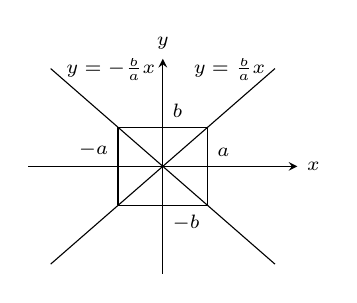
\begin{tikzpicture}[font=\scriptsize,declare function={f(\x)=sqrt(5)/2*sqrt(\x^2-4);fda(\x)=sqrt(5)/2*\x;fdb(\x)=-sqrt(5)/2*\x;}]
\pgfmathsetmacro{\b}{sqrt(5)}
\pgfmathsetmacro{\a}{2}
\pgfmathsetmacro{\n}{\b/2*sqrt(3.5*3.5-4)}
\begin{axis}[width=5cm,axis lines=middle,xlabel={$x$},ylabel={$y$},xlabel style={at={(current axis.right of origin)},anchor=west},ylabel style={at={(current axis.above origin)},anchor=south},xtick={\empty},ytick={\empty},enlargelimits=true, xmin=-5, xmax=5, ymin=-5.123,ymax=5.123]
\addplot[]plot coordinates {(-\a,-\b)(-\a,\b)(\a,\b)(\a,-\b)(-\a,-\b)};
\addplot[]plot coordinates{(-\a,0)}node[above left]{$-a$};
\addplot[]plot coordinates{(\a,0)}node[above right]{$a$};
\addplot[]plot coordinates{(0,\b)}node[above right]{$b$}  {(0,-\b)}node[below right]{$-b$};
\addplot[domain=-5:5]{fda(x)}node[left]{$y=\frac{b}{a}x$};
\addplot[domain=-5:5]{fdb(x)}node[pos=0,right,xshift=0.5ex]{$y=-\frac{b}{a}x$};
\end{axis}
\end{tikzpicture}
\caption{}
\end{subfigure}\hfill
\begin{subfigure}{0.3\textwidth}
\centering
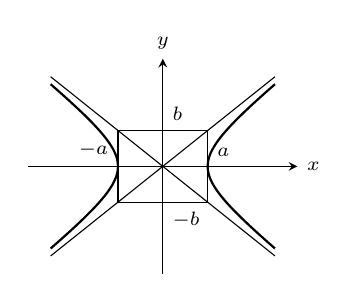
\begin{tikzpicture}[font=\scriptsize,declare function={f(\x)=sqrt(5)/2*sqrt(\x^2-4);fda(\x)=sqrt(5)/2*\x;fdb(\x)=-sqrt(5)/2*\x;}]
\pgfmathsetmacro{\a}{2}
\pgfmathsetmacro{\c}{3}
\pgfmathsetmacro{\b}{sqrt(\c^2-\a^2)}
\pgfmathsetmacro{\n}{\b/2*sqrt(3.5*3.5-4)}
\begin{axis}[width=5cm,axis lines=middle,xlabel={$x$},ylabel={$y$},xlabel style={at={(current axis.right of origin)},anchor=west},ylabel style={at={(current axis.above origin)},anchor=south},xtick={\empty},ytick={\empty},enlargelimits=true]
\addplot[]plot coordinates {(-\a,-\b)(-\a,\b)(\a,\b)(\a,-\b)(-\a,-\b)};
\addplot[]plot coordinates{(-\a,0)}node[above left]{$-a$};
\addplot[]plot coordinates{(\a,0)}node[above right]{$a$};
\addplot[]plot coordinates{(0,\b)}node[above right]{$b$}  {(0,-\b)}node[below right]{$-b$};
\addplot[domain=-5:5]{fda(x)};
\addplot[domain=-5:5]{fdb(x)};
\addplot[thick,domain=2:2.25]{f(x)};
\addplot[thick,domain=2.25:5]{f(x)};
\addplot[thick,domain=2:2.25]{-f(x)};
\addplot[thick,domain=2.25:5]{-f(x)};
\addplot[thick,domain=2:2.25](-x,{f(x)});
\addplot[thick,domain=2.25:5](-x,{f(x)});
\addplot[thick,domain=2:2.25](-x,{-f(x)});
\addplot[thick,domain=2.25:5](-x,{-f(x)});
\end{axis}
\end{tikzpicture}
\caption{}
\end{subfigure}
\caption{متقارب کی مدد سے قطع زائد کی ترسیم۔}
\label{شکل_مخروط_متقارب_سے_قطع_زائد}
\end{figure}

\ابتدا{مثال}\شناخت{مثال_مخروط_ماسکہ_افقی_محور_پر}\ترچھا{محور \عددی{x} پر ماسکے}\\
درج ذیل قطع زائد کی مساوات ہے (شکل \حوالہ{شکل_مثال_مخروط_ماسکہ_افقی_محور_پر})
\begin{align*}
\frac{x^2}{4}-\frac{y^2}{5}=1
\end{align*}
جس میں \عددی{a^2=4} اور \عددی{b^2=5} ہیں (مساوات \حوالہ{مساوات_مخروط_قطع_زائد})۔ یوں درج ذیل ہوں گے۔
\begin{align*}
c&=\sqrt{a^2+b^2}=\sqrt{4+5}=3&&\text{\RL{مرکز سے ماسکہ تک فاصلہ}}\\
(\pm c,0)&=(\pm 3,0)&&\text{ماسکے}\\
(\pm a,0)&=(\pm 2,0)&&\text{راس}\\
y&=\pm \frac{\sqrt{5}}{2}x&&\text{متقارب}
\end{align*}
\انتہا{مثال}
%================
\begin{figure}
\centering
\begin{minipage}{0.45\textwidth}
\centering
\begin{tikzpicture}[declare function={f(\x)=sqrt(5)/2*sqrt(\x^2-4);fd(\x)=sqrt(5/4)*\x;}]
\begin{axis}[clip=false,small,axis lines=middle,xlabel={$x$},ylabel={$y$},xlabel style={at={(current axis.right of origin)},anchor=west}, ylabel style={at={(current axis.above origin)},anchor=south},xtick={\empty},ytick={\empty}]
\addplot[domain=2:2.5]{f(x)};
\addplot[domain=2.5:8]{f(x)};
\addplot[domain=2:2.5]{-f(x)};
\addplot[domain=2.5:8]{-f(x)};
\addplot[domain=2:2.5](-x,{f(x)});
\addplot[domain=2.5:8](-x,{f(x)});
\addplot[domain=2:2.5](-x,{-f(x)});
\addplot[domain=2.5:8](-x,{-f(x)});
\addplot[domain=-8:8]{fd(x)}node[left,yshift=1ex]{$y=\frac{\sqrt{5}}{2}x$};
\addplot[domain=-8:8]{-fd(x)}node[pos=0,right,yshift=1ex]{$y=-\frac{\sqrt{5}}{2}x$};
\addplot[]plot coordinates {(3,0)}node[circ]{}node[above right]{$F(3,0)$}   {(-3,0)}node[circ]{}node[above left]{$F(-3,0)$};
\addplot[]plot coordinates {(2,0)}node[circ]{}node[pin=-40:{$2$}]{}  {(-2,0)}node[circ]{}node[pin=-140:{$-2$}]{};
\addplot[]plot coordinates {(4,4)}node[right,font=\scriptsize]{$\frac{x^2}{4}-\frac{y^2}{5}=1$};
\end{axis}
\end{tikzpicture}
\caption{قطع زائد (مثال \حوالہ{مثال_مخروط_ماسکہ_افقی_محور_پر})}
\label{شکل_مثال_مخروط_ماسکہ_افقی_محور_پر}
\end{minipage}\hfill
\begin{minipage}{0.45\textwidth}
\centering
\begin{tikzpicture}[declare function={f(\x)=2/sqrt(5)*sqrt(\x^2+5);fd(\x)=sqrt(4/5)*\x;}]
\begin{axis}[clip=false,small,axis lines=middle,xlabel={$x$},ylabel={$y$},xlabel style={at={(current axis.right of origin)},anchor=west}, ylabel style={at={(current axis.above origin)},anchor=south},xtick={\empty},ytick={\empty}]
\addplot[domain=-6:6]{f(x)};
\addplot[domain=-6:6]{-f(x)};
\addplot[domain=-6:6]{fd(x)}node[pos=0.75,right,yshift=-0.5ex]{$y=\frac{2}{\sqrt{5}}x$};
\addplot[domain=-6:6]{-fd(x)}node[pos=0.25,left,yshift=-0.5ex]{$y=-\frac{2}{\sqrt{5}}x$};
\addplot[]plot coordinates {(0,3)}node[circ]{}node[above right]{$F(0,3)$}   {(0,-3)}node[circ]{}node[below right]{$F(0,-3)$};
\addplot[]plot coordinates {(0,2)}node[circ]{}node[below left]{$2$}  {(0,-2)}node[circ]{}node[above left]{$-2$};
\addplot[]plot coordinates {(1,5)}node[above right]{$\frac{y^2}{4}-\frac{x^2}{5}=1$};
\end{axis}
\end{tikzpicture}
\caption{قطع زائد (مثال \حوالہ{مثال_مخروط_ماسکہ_عمودی_محور_پر})}
\label{شکل_مثال_مخروط_ماسکہ_عمودی_محور_پر}
\end{minipage}
\end{figure}

\ابتدا{مثال}\شناخت{مثال_مخروط_ماسکہ_عمودی_محور_پر}
درج ذیل قطع زائد کو  مثال \حوالہ{مثال_مخروط_ماسکہ_افقی_محور_پر} کے قطع زائد میں \عددی{x} اور \عددی{y} کو ایک دوسرے کے ساتھ بدل کر حاصل کیا گیا ہے۔ 
\begin{align*}
\frac{y^2}{4}-\frac{x^2}{5}=1
\end{align*}
اس قطع زائد کے راس عمودی محور پر پائے جائیں گے (شکل \حوالہ{شکل_مثال_مخروط_ماسکہ_عمودی_محور_پر})۔ اب بھی \عددی{a^2=4} اور \عددی{b^2=5} ہوں گے۔یوں درج ذیل ہو گا۔
\begin{align*}
c&=\sqrt{a^2+b^2}=\sqrt{4+5}=3&&\text{\RL{مرکز سے ماسکہ تک فاصلہ}}\\
(0,\pm c)&=(0,\pm 3)&&\text{ماسکے}\\
(0,\pm a)&=(0,\pm 2)&&\text{راس}\\
&(0,0)&&\text{مرکز}\\
y&=\pm \frac{2}{\sqrt{5}}x&&\text{متقارب}
\end{align*}
\انتہا{مثال}
%==================

\جزوحصہء{عکسی خواص}
قطع مکافی کا اہم ترین استعمال بطور  شعاع اور ریڈیو امواج کا عاکس ہے۔ قطع مکافی کے ماسکہ سے خارج شعاع، قطع مکافی کے محور کے متوازی منعکس ہوتا ہے (شکل \حوالہ{شکل_مخروط_قطع_مکافی_آئینہ_خاصیت})۔ یہ خاصیت ہاتھ بتی اور گاڑیوں کی اگلی بتیوں میں بروئے کار لایا جاتا ہے۔ اس کے علاوہ خرد امواج نشر کرنے کے لئے بھی قطع مکافی اینٹینا استعمال کیا جاتا ہے جو نقطہ منبع سے خارج برقناطیسی امواج کو ایک محدود شعاع  کی صورت میں خارج کرتا ہے۔ اس کے برعکس قطع مکافی عاکس کے محور کے متوازی آمد  برقناطیسی امواج عاکس کے ماسکہ پر مرکوز کیے جاتے ہیں (شکل \حوالہ{شکل_مخروط_دور_بینی_آئینہ})۔اس خاصیت کی بنا ٹیلی وژن کا ڈش اینٹینا یا ریڈیو دوربین  کمزور اشارات کو اکٹھے کر کے زیادہ طاقتور اشارہ حاصل کرتا ہے۔
اسی طرح سورج کی روشنی کو ایک نقطہ پر مرتکز کیا جا سکتا ہے۔

\begin{figure}
\centering
\begin{minipage}{0.3\textwidth}
\centering
\begin{tikzpicture}[declare function={f(\x)=2*(\x)^2;}]
\pgfmathsetmacro{\a}{0.15}
\pgfmathsetmacro{\b}{0.3}
\pgfmathsetmacro{\c}{0.45}
\begin{axis}[axis equal,width=5cm, axis line style={draw=none},tick style={draw=none},xtick={\empty},ytick={\empty}]
\addplot[thick,domain=0:0.62]({f(x)},x);
\addplot[thick,domain=0:0.62]({f(x)},-x);
\addplot[]plot coordinates{(0.5,0)}node[circ]{};
\addplot[->-=0.75]plot coordinates  {(0.5,0)({f(\a)},\a)};
\addplot[->-=0.75]plot coordinates  {({f(\a)},\a)(1.5,\a)};
\addplot[->-=0.75]plot coordinates  {(0.5,0)({f(\b)},\b)};
\addplot[->-=0.75]plot coordinates  {({f(\b)},\b)(1.5,\b)};
\addplot[->-=0.75]plot coordinates  {(0.5,0)({f(\c)},\c)};
\addplot[->-=0.75]plot coordinates  {({f(\c)},\c)(1.5,\c)};
\addplot[->-=0.75]plot coordinates  {(0.5,0)({f(\a)},-\a)};
\addplot[->-=0.75]plot coordinates  {({f(\a)},-\a)(1.5,-\a)};
\addplot[->-=0.75]plot coordinates  {(0.5,0)({f(\b)},-\b)};
\addplot[->-=0.75]plot coordinates  {({f(\b)},-\b)(1.5,-\b)};
\addplot[->-=0.75]plot coordinates  {(0.5,0)({f(\c)},-\c)};
\addplot[->-=0.75]plot coordinates  {({f(\c)},-\c)(1.5,-\c)};
\end{axis}
\end{tikzpicture}
\caption{قطع مکافی آئینہ کے ماسکہ سے نکلتا شعاع انعکاس کے بعد محور کے متوازی ہو گا۔}
\label{شکل_مخروط_قطع_مکافی_آئینہ_خاصیت}
\end{minipage}\hfill
\begin{minipage}{0.3\textwidth}
\centering
\begin{tikzpicture}[declare function={f(\x)=2*(\x)^2;}]
\pgfmathsetmacro{\a}{0.15}
\pgfmathsetmacro{\b}{0.3}
\pgfmathsetmacro{\c}{0.45}
\begin{scope}[rotate=30]
\begin{axis}[axis equal,width=5cm, axis line style={draw=none},tick style={draw=none},xtick={\empty},ytick={\empty}]
\addplot[thick,domain=0:0.62]({f(x)},x);
\addplot[thick,domain=0:0.62]({f(x)},-x);
\addplot[]plot coordinates{(0.5,0)}node[circ]{};
\addplot[-<-=0.75]plot coordinates  {(0.5,0)({f(\a)},\a)};
\addplot[-<-=0.75]plot coordinates  {({f(\a)},\a)(1.5,\a)};
\addplot[-<-=0.75]plot coordinates  {(0.5,0)({f(\b)},\b)};
\addplot[-<-=0.75]plot coordinates  {({f(\b)},\b)(1.5,\b)};
\addplot[-<-=0.75]plot coordinates  {(0.5,0)({f(\c)},\c)};
\addplot[-<-=0.75]plot coordinates  {({f(\c)},\c)(1.5,\c)};
\addplot[-<-=0.75]plot coordinates  {(0.5,0)({f(\a)},-\a)};
\addplot[-<-=0.75]plot coordinates  {({f(\a)},-\a)(1.5,-\a)};
\addplot[-<-=0.75]plot coordinates  {(0.5,0)({f(\b)},-\b)};
\addplot[-<-=0.75]plot coordinates  {({f(\b)},-\b)(1.5,-\b)};
\addplot[-<-=0.75]plot coordinates  {(0.5,0)({f(\c)},-\c)};
\addplot[-<-=0.75]plot coordinates  {({f(\c)},-\c)(1.5,-\c)};
\end{axis}
\end{scope}
\end{tikzpicture}
\caption{قطع مکافی عاکس پر آمد شعاع ماسکہ پر پہنچتا ہے۔}
\label{شکل_مخروط_دور_بینی_آئینہ}
\end{minipage}\hfill
\begin{minipage}{0.3\textwidth}
\centering
\begin{tikzpicture}[declare function={f(\x)=1.5/2*sqrt(2^2-(\x)^2);}]
\pgfmathsetmacro{\c}{sqrt(2^2-1.5^2)}
\begin{axis}[axis equal,width=5cm,axis line style={draw=none},tick style={draw=none},xtick={\empty},ytick=\empty]
\addplot[thick,domain=-2:-2+0.2]{f(x)};
\addplot[thick,domain=-2+0.2:2-0.2]{f(x)};
\addplot[thick,domain=2-0.2:2]{f(x)};
\addplot[thick,domain=-2:-2+0.2]{-f(x)};
\addplot[thick,domain=-2+0.2:2-0.2]{-f(x)};
\addplot[thick,domain=2-0.2:2]{-f(x)};
\addplot[]plot coordinates{(-\c,0)}node[circ]{}node[below]{$F_1$};
\addplot[]plot coordinates{(\c,0)}node[circ]{}node[below]{$F_2$};
\addplot[->-=0.5]plot coordinates {(-\c,0)(1.3,{f(1.3)})};
\addplot[->-=0.5]plot coordinates {(1.3,{f(1.3)})(\c,0)};
\end{axis}
\end{tikzpicture}
\caption{ترخیم کے ایک ماسکہ سے خارج شعاع دوسرے ماسکہ پر پہنچتا ہے۔}
\label{شکل_مخروط_ترخیم_کمرہ_سرگوشی}
\end{minipage}
\end{figure}

ایک ترخیم کو اس کے محور کے گرد گھما کر سطح طواف پیدا کیا جا سکتا ہے جو \اصطلاح{ترخیمی سطح}\فرہنگ{ترخیمی سطح}\حاشیہب{ellipsoid}\فرہنگ{ellipsoid} کہلاتا ہے۔اس کی اندرونی سطح پر چاندی کی تہہ لگا کر آئینہ بنایا جا سکتا ہے۔ ایک ماسکہ سے خارج شعاع دوسرے ماسکہ پر منعکس ہو گا (شکل \حوالہ{شکل_مخروط_ترخیم_کمرہ_سرگوشی} اور سوال \حوالہ{سوال_مخروط_کمرہ_سرگوشی})۔ ترخیمی سطح اسی طرح آواز کو بھی ایک ماسکہ سے دوسرے ماسکہ منتقل کرتا ہے۔ اس خاصیت کو استعمال کرتے ہوئے کمرہ سرگوشی بنایا جا سکتا ہے جس میں ایک ماسکہ پر بیٹھا شخص دوسرے ماسکہ پر بیٹھے شخص کے ساتھ سرگوشی سے باتیں کر سکتا ہے۔ کمرہ سرگوشی میں موجود باقی لوگ ان کی باتیں سننے  سے قاصر ہوں  گے۔ ہوائی جہازوں کی کارکردگی پر ہوائی سرنگ میں غور کیا جاتا ہے۔ جہاز کے شور پر غور کرتے ہوئے نقطہ غور کو ترخیمی سطح کے ایک ماسکہ پر رکھا جاتا ہے جبکہ مائکروفون  کو  اس کی دوسرے ماسکہ پر رکھا جاتا ہے۔ دیگر نقطوں سے پیدا شور کے اثر کو یوں بہت کم کرنا ممکن ہوتا ہے۔

قطع زائد آئینہ کے ایک ماسکہ پر آمد شعاع کو آئینہ دوسرے ماسکہ پر بھیجتا ہے۔ قطع مکافی سطح، ترخیمی سطح اور قطع مکافی سطحوں کے خواص کو استعمال کرتے ہوئے جدید دور بین تیار کیے جاتے ہیں۔   

\جزوحصہء{سوالات}
\موٹا{ترسیم کی پہچان}\\
سوال \حوالہ{سوال_مخروط_ہم_پلہ_الف} تا سوال \حوالہ{سوال_مخروط_ہم_پلہ_ب} میں دی  گئی قطع مکافی کی مساوات درج ذیل میں تلاش کریں۔
\begin{align*}
x^2=2y,\quad x^2=-6y,\quad y^2=8x,\quad y^2=-4x
\end{align*}
اس کے بعد قطع مکافی کے ماسکہ اور ناظمہ دریافت کریں۔

%=============================
\ابتدا{سوال}\شناخت{سوال_مخروط_ہم_پلہ_الف}
شکل \حوالہ{شکل_مخروط_ترخیم_بائیں_دائیں}-ا\\
جواب:\quad
\عددی{y^2=8x}، ماسکہ \عددی{F(2,0)} اور ناظمہ \عددی{x=-2}
\انتہا{سوال}
%===================
\ابتدا{سوال}
شکل \حوالہ{شکل_مخروط_ترخیم_بائیں_دائیں}-ب
\انتہا{سوال}
%===================
\ابتدا{سوال}
شکل \حوالہ{شکل_مخروط_ترخیم_بائیں_دائیں}-ج\\
جواب:\quad
\عددی{x^2=-6y}، ماسکہ \عددی{F(0,-\tfrac{3}{2})} اور ناظمہ \عددی{y=\tfrac{3}{2}}
\انتہا{سوال}
%===================
\ابتدا{سوال}\شناخت{سوال_مخروط_ہم_پلہ_ب}
شکل \حوالہ{شکل_مخروط_ترخیم_بائیں_دائیں}-د
\انتہا{سوال}
%===================
\begin{figure}
\centering
\begin{subfigure}{0.22\textwidth}
\centering
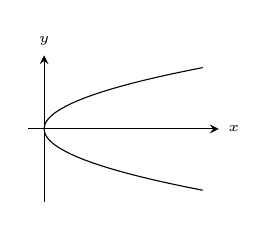
\begin{tikzpicture}[font=\tiny,declare function={f(\x)=2*sqrt(\x);}]
\begin{axis}[width=4cm,axis lines=middle,xlabel={$x$},ylabel={$y$},xlabel style={at={(current axis.right of origin)},anchor=west},ylabel style={at={(current axis.above origin)},anchor=south},xtick={\empty},ytick={\empty},enlargelimits]
\addplot[domain=0:0.2]{f(x)};
\addplot[domain=0.2:2]{f(x)};
\addplot[domain=0:0.2]{-f(x)};
\addplot[domain=0.2:2]{-f(x)};
\end{axis}
\end{tikzpicture}
\caption{}
\end{subfigure}\hfill
\begin{subfigure}{0.22\textwidth}
\centering
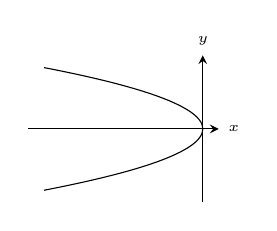
\begin{tikzpicture}[font=\tiny,declare function={f(\x)=2*sqrt(-\x);}]
\begin{axis}[width=4cm,axis lines=middle,xlabel={$x$},ylabel={$y$},xlabel style={at={(current axis.right of origin)},anchor=west},ylabel style={at={(current axis.above origin)},anchor=south},xtick={\empty},ytick={\empty},enlargelimits=true]
\addplot[domain=0:-0.2]{f(x)};
\addplot[domain=-0.2:-2]{f(x)};
\addplot[domain=0:-0.2]{-f(x)};
\addplot[domain=-0.2:-2]{-f(x)};
\end{axis}
\end{tikzpicture}
\caption{}
\end{subfigure}\hfill
\begin{subfigure}{0.22\textwidth}
\centering
\begin{tikzpicture}[font=\tiny,declare function={f(\x)=-1/4*\x^2;}]
\begin{axis}[width=4cm,axis lines=middle,xlabel={$x$},ylabel={$y$},xlabel style={at={(current axis.right of origin)},anchor=west},ylabel style={at={(current axis.above origin)},anchor=south},xtick={\empty},ytick={\empty},enlargelimits]
\addplot[domain=0:0.2]{f(x)};
\addplot[domain=0.2:2]{f(x)};
\addplot[domain=0:0.2](-x,{f(x)});
\addplot[domain=0.2:2](-x,{f(x)});
\end{axis}
\end{tikzpicture}
\caption{}
\end{subfigure}\hfill
\begin{subfigure}{0.22\textwidth}
\centering
\begin{tikzpicture}[font=\tiny,declare function={f(\x)=1/4*\x^2;}]
\begin{axis}[width=4cm,axis lines=middle,xlabel={$x$},ylabel={$y$},xlabel style={at={(current axis.right of origin)},anchor=west},ylabel style={at={(current axis.above origin)},anchor=south},xtick={\empty},ytick={\empty},enlargelimits=true]
\addplot[domain=0:0.2]{f(x)};
\addplot[domain=0.2:2]{f(x)};
\addplot[domain=0:0.2](-x,{f(x)});
\addplot[domain=0.2:2](-x,{f(x)});
\end{axis}
\end{tikzpicture}
\caption{}
\end{subfigure}
\caption{ترسیم برائے سوال \حوالہ{سوال_مخروط_ہم_پلہ_الف} تا سوال \حوالہ{سوال_مخروط_ہم_پلہ_ب}}
\label{شکل_مخروط_ترخیم_بائیں_دائیں}
\end{figure}

سوال \حوالہ{سوال_مخروط_ہم_پلہ_تلاش_الف} تا سوال \حوالہ{سوال_مخروط_ہم_پلہ_تلاش_ب} میں دیے گئے مخروط کی مساوات درج ذیل میں تلاش کریں۔
\begin{align*}
\frac{x^2}{4}+\frac{y^2}{9}=1,\quad \frac{x^2}{2}+y^2=1,\quad \frac{y^2}{4}-x^2=1,\quad \frac{x^2}{4}-\frac{y^2}{9}=1
\end{align*}
دیے گئے مخروط کا ماسکہ اور راس تلاش کریں۔ اگر قطع زائد دیا گیا ہو تب اس کے متقارب بھی دریافت کریں۔

\ابتدا{سوال}\شناخت{سوال_مخروط_ہم_پلہ_تلاش_الف}
ترسیم شکل \حوالہ{شکل_مخروط_کئی_الف}-ا میں دیا گیا ہے۔\\
جواب:\quad
\عددی{\tfrac{x^2}{4}-\tfrac{y^2}{9}=1}، ماسکے \عددی{F(\pm\sqrt{13},0)}، راس \عددی{V(\pm 2,0)} اور متقارب \عددی{y=\pm\tfrac{3}{2}x}
\انتہا{سوال}
%===================
\ابتدا{سوال}
ترسیم شکل \حوالہ{شکل_مخروط_کئی_الف}-ب میں دیا گیا ہے۔
\انتہا{سوال}
%========================
\ابتدا{سوال}
ترسیم شکل \حوالہ{شکل_مخروط_کئی_الف}-ج میں دیا گیا ہے۔\\
جواب:\quad
\عددی{\tfrac{x^2}{2}+y^2=1}، ماسکے \عددی{F(\pm 1,0)}، راس \عددی{V(\pm\sqrt{2},0)}
\انتہا{سوال}
%========================
\ابتدا{سوال}\شناخت{سوال_مخروط_ہم_پلہ_تلاش_ب}
ترسیم شکل \حوالہ{شکل_مخروط_کئی_الف}-د میں دیا گیا ہے۔
\انتہا{سوال}
%========================
\begin{figure}
\centering
\begin{subfigure}{0.22\textwidth}
\centering
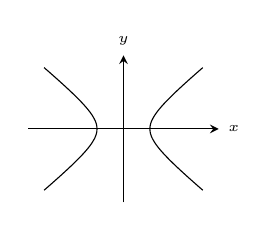
\begin{tikzpicture}[font=\tiny,declare function={f(\x)=sqrt(5)/2*sqrt(\x^2-4);}]
\begin{axis}[width=4cm,axis lines=middle,xlabel={$x$},ylabel={$y$},xlabel style={at={(current axis.right of origin)},anchor=west},ylabel style={at={(current axis.above origin)},anchor=south},xtick={\empty},ytick={\empty},enlargelimits]
\addplot[domain=2:2.2]{f(x)};
\addplot[domain=2.2:6]{f(x)};
\addplot[domain=2:2.2]{-f(x)};
\addplot[domain=2.2:6]{-f(x)};
\addplot[domain=2:2.2](-x,{f(x)});
\addplot[domain=2.2:6](-x,{f(x)});
\addplot[domain=2:2.2](-x,{-f(x)});
\addplot[domain=2.2:6](-x,{-f(x)});
\end{axis}
\end{tikzpicture}
\caption{}
\end{subfigure}\hfill
\begin{subfigure}{0.22\textwidth}
\centering
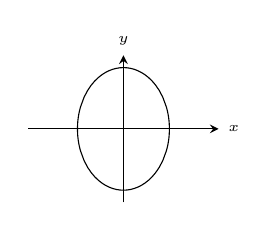
\begin{tikzpicture}[font=\tiny,declare function={f(\x)=4/3*sqrt(9-\x^2);}]
\begin{axis}[width=4cm,axis equal,axis lines=middle,xlabel={$x$},ylabel={$y$},xlabel style={at={(current axis.right of origin)},anchor=west},ylabel style={at={(current axis.above origin)},anchor=south},xtick={\empty},ytick={\empty},enlargelimits]
\addplot[domain=-3:-2.8]{f(x)};
\addplot[domain=-2.8:2.8]{f(x)};
\addplot[domain=2.8:3]{f(x)};
\addplot[domain=-3:-2.8]{-f(x)};
\addplot[domain=-2.8:2.8]{-f(x)};
\addplot[domain=2.8:3]{-f(x)};
\end{axis}
\end{tikzpicture}
\caption{}
\end{subfigure}\hfill
\begin{subfigure}{0.22\textwidth}
\centering
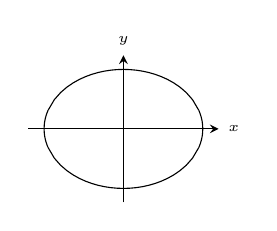
\begin{tikzpicture}[font=\tiny,declare function={f(\x)=3/4*sqrt(16-\x^2);}]
\begin{axis}[width=4cm,axis equal,axis lines=middle,xlabel={$x$},ylabel={$y$},xlabel style={at={(current axis.right of origin)},anchor=west},ylabel style={at={(current axis.above origin)},anchor=south},xtick={\empty},ytick={\empty},enlargelimits]
\addplot[domain=-4:-3.8]{f(x)};
\addplot[domain=-3.8:3.8]{f(x)};
\addplot[domain=3.8:4]{f(x)};
\addplot[domain=-4:-3.8]{-f(x)};
\addplot[domain=-3.8:3.8]{-f(x)};
\addplot[domain=3.8:4]{-f(x)};
\end{axis}
\end{tikzpicture}
\caption{}
\end{subfigure}\hfill
\begin{subfigure}{0.22\textwidth}
\centering
\begin{tikzpicture}[font=\tiny,declare function={f(\x)=2/sqrt(5)*sqrt(5+\x^2);}]
\begin{axis}[width=4cm,axis equal,axis lines=middle,xlabel={$x$},ylabel={$y$},xlabel style={at={(current axis.right of origin)},anchor=west},ylabel style={at={(current axis.above origin)},anchor=south},xtick={\empty},ytick={\empty},enlargelimits]
\addplot[domain=-4:4]{f(x)};
\addplot[domain=-4:4]{-f(x)};
\end{axis}
\end{tikzpicture}
\caption{}
\end{subfigure}
\caption{ترسیمات برائے سوال \حوالہ{سوال_مخروط_ہم_پلہ_تلاش_الف} تا سوال \حوالہ{سوال_مخروط_ہم_پلہ_تلاش_ب}}
\label{شکل_مخروط_کئی_الف}
\end{figure}

\موٹا{قطع مکافی}\\
سوال \حوالہ{سوال_مخروط_قطع_مکافی_دیا_الف} تا سوال \حوالہ{سوال_مخروط_قطع_مکافی_دیا_ٹ} میں دیے گئے قطع مکافی کا ماسکہ اور ناظمہ تلاش کرنے کے بعد  اس کو ترسیم کریں۔ ماسکہ اور ناظمہ کو بھی ترسیم میں شامل کریں۔

\ابتدا{سوال}\شناخت{سوال_مخروط_قطع_مکافی_دیا_الف}
$y^2=12x$\\
جواب:\quad
شکل \حوالہ{شکل_سوال_مخروط_قطع_مکافی_دیا_الف}
\انتہا{سوال}
%=====================
\ابتدا{سوال}
$x^2=6y$
\انتہا{سوال}
%=====================
\ابتدا{سوال}\شناخت{سوال_مخروط_قطع_مکافی_دیا_ب}
$x^2=-8y$\\
جواب:\quad
شکل \حوالہ{شکل_سوال_مخروط_قطع_مکافی_دیا_ب}
\انتہا{سوال}
%=====================
\ابتدا{سوال}
$y^2=-2x$
\انتہا{سوال}
%=====================
\ابتدا{سوال}\شناخت{سوال_مخروط_قطع_مکافی_دیا_پ}
$y=4x^2$\\
جواب:\quad
شکل \حوالہ{شکل_سوال_مخروط_قطع_مکافی_دیا_پ}
\انتہا{سوال}
%=====================
\ابتدا{سوال}
$y=-8x^2$
\انتہا{سوال}
%=====================
\ابتدا{سوال}\شناخت{سوال_مخروط_قطع_مکافی_دیا_ت}
$x=-3y^2$\\
جواب:\quad
شکل \حوالہ{شکل_سوال_مخروط_قطع_مکافی_دیا_ت}
\انتہا{سوال}
%=====================
\ابتدا{سوال}\شناخت{سوال_مخروط_قطع_مکافی_دیا_ٹ}
$x=2y^2$
\انتہا{سوال}
%=====================
\begin{figure}
\centering
\begin{minipage}{0.22\textwidth}
\begin{tikzpicture}[font=\tiny,declare function={f(\x)=sqrt(12*\x);}]
\begin{axis}[clip=false,width=4cm,axis lines=middle,xlabel={$x$},ylabel={$y$},xlabel style={at={(current axis.right of origin)},anchor=west},ylabel style={at={(current axis.above origin)},anchor=south},enlargelimits=true,xtick={-3},ytick={3}]
\addplot[domain=0:0.2]{f(x)};
\addplot[domain=0.2:4]{f(x)}node[pos=0.75,below right]{$y^2=12x$};
\addplot[domain=0:0.2]{-f(x)};
\addplot[domain=0.2:4]{-f(x)};
\addplot[]plot coordinates {(-3,-7)(-3,7)}node[pos=0.85,right]{$x=-3$};
\addplot[]plot coordinates {(3,0)}node[circ]{}node[below]{$F(3,0)$};
\end{axis}
\end{tikzpicture}
\caption{}
\label{شکل_سوال_مخروط_قطع_مکافی_دیا_الف}
\end{minipage}\hfill
\begin{minipage}{0.22\textwidth}
\begin{tikzpicture}[font=\tiny,declare function={f(\x)=-1/8*(\x)^2;}]
\begin{axis}[width=4cm,axis lines=middle,xlabel={$x$},ylabel={$y$},xlabel style={at={(current axis.right of origin)},anchor=west},ylabel style={at={(current axis.above origin)},anchor=south},enlargelimits=true,xtick={2},ytick={2},y tick label style={yshift=0.5ex}]
\addplot[domain=-3:3]{f(x)}node[pos=0.25,below,yshift=-0.5ex]{$x^2=-8y$};
\addplot[]plot coordinates {(-3,2)(3,2)}node[pos=0.85,below]{$y=2$};
\addplot[]plot coordinates {(0,-2)}node[circ]{}node[right]{$F(0,-2)$};
\end{axis}
\end{tikzpicture}
\caption{}
\label{شکل_سوال_مخروط_قطع_مکافی_دیا_ب}
\end{minipage}\hfill
\begin{minipage}{0.22\textwidth}
\begin{tikzpicture}[font=\tiny,declare function={f(\x)=4*(\x)^2;}]
\pgfmathsetmacro{\d}{1/16}
\begin{axis}[clip=false,width=4cm,axis lines=middle,xlabel={$x$},ylabel={$y$},xlabel style={at={(current axis.right of origin)},anchor=west},ylabel style={at={(current axis.above origin)},anchor=south},enlargelimits=true,xtick={0.25},ytick={0.25},xticklabels={$\tfrac{1}{4}$},yticklabels={$\tfrac{1}{4}$}]
\addplot[domain=-0.3:0.3]{f(x)}node[left]{$y=4x^2$};
\addplot[]plot coordinates {(-0.3,-\d)(0.3,-\d)}node[pos=0.15,below]{$y=-\tfrac{1}{16}$};
\addplot[]plot coordinates {(0,\d)}node[circ]{}node[right]{$F(0,\tfrac{1}{16})$};
\end{axis}
\end{tikzpicture}
\caption{}
\label{شکل_سوال_مخروط_قطع_مکافی_دیا_پ}
\end{minipage}\hfill
\begin{minipage}{0.22\textwidth}
\begin{tikzpicture}[font=\tiny,declare function={f(\x)=sqrt(-1/3*\x);}]
\pgfmathsetmacro{\d}{1/12}
\pgfmathsetmacro{\yt}{1/6}
\begin{axis}[clip=false,width=4cm,axis lines=middle,xlabel={$x$},ylabel={$y$},xlabel style={at={(current axis.right of origin)},anchor=west},ylabel style={at={(current axis.above origin)},anchor=south},enlargelimits=true,xtick={\d},ytick={-\yt,\yt},xticklabels={\hspace*{2ex}$\tfrac{1}{12}$},yticklabels={$-\tfrac{1}{6}$,$\tfrac{1}{6}$}]
\addplot[domain=-0.15:0]{f(x)}node[pos=0,below]{$x=-3y^2$};
\addplot[domain=-0.15:0]{-f(x)};
\addplot[]plot coordinates {(\d,-0.2)(\d,0.2)}node[above]{$x=\tfrac{1}{12}$};
\addplot[]plot coordinates {(-\d,0)}node[circ]{}node[below]{$F(-\tfrac{1}{12},0)$};
\end{axis}
\end{tikzpicture}
\caption{}
\label{شکل_سوال_مخروط_قطع_مکافی_دیا_ت}
\end{minipage}
\end{figure}
\موٹا{ترخیم}\\
سوال \حوالہ{سوال_مخروط_ترخیم_دیا_الف} تا سوال \حوالہ{سوال_مخروط_ترخیم_دیا_ٹ} میں دیے گئے ترخیم کی مساوات کو معیاری روپ میں لکھ کر ترسیم کریں۔ ترسیم پر ماسکے  دکھائیں۔ 

\ابتدا{سوال}\شناخت{سوال_مخروط_ترخیم_دیا_الف}
$16x^2+25y^2=400$\\
جواب:\quad
شکل \حوالہ{شکل_سوال_مخروط_ترخیم_دیا_الف}
\انتہا{سوال}
%===================
\ابتدا{سوال}
$7x^2+16y^2=112$
\انتہا{سوال}
%=====================
\ابتدا{سوال}\شناخت{سوال_مخروط_ترخیم_دیا_ب}
$2x^2+y^2=2$\\
جواب:\quad
شکل \حوالہ{شکل_سوال_مخروط_ترخیم_دیا_ب}
\انتہا{سوال}
%=====================
\ابتدا{سوال}
$2x^2+y^2=4$
\انتہا{سوال}
%=====================
\ابتدا{سوال}\شناخت{سوال_مخروط_ترخیم_دیا_پ}
$3x^2+2y^2=6$\\
جواب:\quad
شکل \حوالہ{شکل_سوال_مخروط_ترخیم_دیا_پ}
\انتہا{سوال}
%=====================
\ابتدا{سوال}
$9x^2+10y^2=90$
\انتہا{سوال}
%=====================
\ابتدا{سوال}\شناخت{سوال_مخروط_ترخیم_دیا_ت}
$6x^2+9y^2=54$\\
جواب:\quad
شکل \حوالہ{شکل_سوال_مخروط_ترخیم_دیا_ت}
\انتہا{سوال}
%=====================
\ابتدا{سوال}\شناخت{سوال_مخروط_ترخیم_دیا_ٹ}
$169x^2+25y^2=4225$
\انتہا{سوال}
%=====================
\begin{figure}
\centering
\begin{minipage}{0.22\textwidth}
\begin{tikzpicture}[font=\tiny,declare function={f(\x)=4/5*sqrt(25-(\x)^2);}]
\begin{axis}[clip=false,width=4cm,axis lines=middle,xlabel={$x$},ylabel={$y$},xlabel style={at={(current axis.right of origin)},anchor=west},ylabel style={at={(current axis.above origin)},anchor=south},enlargelimits=true,xtick={-3,3},ytick={-4,4}]
\addplot[domain=-4.8:4.8]{f(x)}node[pos=0.8,above,xshift=1ex]{$\tfrac{x^2}{25}+\tfrac{y^2}{16}=1$};
\addplot[domain=-4.8:4.8]{-f(x)};
\addplot[domain=-5:-4.8]{f(x)};
\addplot[domain=-5:-4.8]{-f(x)};
\addplot[domain=4.8:5]{f(x)};
\addplot[domain=4.8:5]{-f(x)};
\addplot[]plot coordinates {(-3,0)}node[above]{$F_1$}  {(3,0)}node[above]{$F_2$};
\end{axis}
\end{tikzpicture}
\caption{}
\label{شکل_سوال_مخروط_ترخیم_دیا_الف}
\end{minipage}\hfill
\begin{minipage}{0.22\textwidth}
\begin{tikzpicture}[font=\tiny,declare function={f(\x)=sqrt(2-2*(\x)^2);}]
\pgfmathsetmacro{\k}{sqrt(2)}
\begin{axis}[axis equal,clip=false,width=4cm,axis lines=middle,xlabel={$x$},ylabel={$y$},xlabel style={at={(current axis.right of origin)},anchor=west},ylabel style={at={(current axis.above origin)},anchor=south},enlargelimits=true,xtick={-1,1},ytick={-1,1}]
\addplot[domain=-0.8:0.8]{f(x)}node[pos=0.75,above,xshift=3ex]{$x^2+\tfrac{y^2}{2}=1$};
\addplot[domain=-0.8:0.8]{-f(x)};
\addplot[domain=-1:-0.8]{f(x)};
\addplot[domain=0.8:1]{f(x)};
\addplot[domain=-1:-0.8]{-f(x)};
\addplot[domain=0.8:1]{-f(x)};
\addplot[]plot coordinates {(0,1)}node[right]{$F_1$}  {(0,-1)}node[right]{$F_2$};
\addplot[]plot coordinates {(0,\k)}node[shift={(-2ex,0.25ex)}]{$\sqrt{2}$};
\end{axis}
\end{tikzpicture}
\caption{}
\label{شکل_سوال_مخروط_ترخیم_دیا_ب}
\end{minipage}\hfill
\begin{minipage}{0.22\textwidth}
\begin{tikzpicture}[font=\tiny,declare function={f(\x)=sqrt(3/2)*sqrt(2-(\x)^2);}]
\pgfmathsetmacro{\k}{sqrt(2)}
\pgfmathsetmacro{\kk}{sqrt(3)}
\begin{axis}[axis equal,clip=false,width=4cm,axis lines=middle,xlabel={$x$},ylabel={$y$},xlabel style={at={(current axis.right of origin)},anchor=west},ylabel style={at={(current axis.above origin)},anchor=south},enlargelimits=true,xtick={\empty},ytick={-1,1}]
\addplot[domain=-\k+0.2:\k-0.2]{f(x)}node[pos=0.75,above,xshift=3ex]{$\tfrac{x^2}{2}+\tfrac{y^2}{3}=1$};
\addplot[domain=-\k+0.2:\k-0.2]{-f(x)};
\addplot[domain=-\k:-\k+0.2]{f(x)};
\addplot[domain=\k-0.2:\k]{f(x)};
\addplot[domain=-\k:-\k+0.2]{-f(x)};
\addplot[domain=\k-0.2:\k]{-f(x)};
\addplot[]plot coordinates {(0,1)}node[right]{$F_1$}  {(0,-1)}node[right]{$F_2$};
\addplot[]plot coordinates {(\k,0)}node[shift={(1ex,-1ex)}]{$\sqrt{2}$}  {(0,\kk)}node[shift={(-2ex,0.25ex)}]{$\sqrt{3}$};
\end{axis}
\end{tikzpicture}
\caption{}
\label{شکل_سوال_مخروط_ترخیم_دیا_پ}
\end{minipage}\hfill
\begin{minipage}{0.22\textwidth}
\begin{tikzpicture}[font=\tiny,declare function={f(\x)=sqrt(6/9)*sqrt(9-(\x)^2);}]
\pgfmathsetmacro{\k}{sqrt(9)}
\pgfmathsetmacro{\kk}{sqrt(6)}
\pgfmathsetmacro{\kkk}{sqrt(3)}
\begin{axis}[axis equal,clip=false,width=4cm,axis lines=middle,xlabel={$x$},ylabel={$y$},xlabel style={at={(current axis.right of origin)},anchor=west},ylabel style={at={(current axis.above origin)},anchor=south},enlargelimits=true,xtick={-\kkk,\kkk},xticklabels={$-\sqrt{3}$,$\sqrt{3}$},ytick={\empty}]
\addplot[domain=-\k+0.2:\k-0.2]{f(x)}node[pos=0.75,above,xshift=3ex]{$\tfrac{x^2}{9}+\tfrac{y^2}{6}=1$};
\addplot[domain=-\k+0.2:\k-0.2]{-f(x)};
\addplot[domain=-\k:-\k+0.2]{f(x)};
\addplot[domain=\k-0.2:\k]{f(x)};
\addplot[domain=-\k:-\k+0.2]{-f(x)};
\addplot[domain=\k-0.2:\k]{-f(x)};
\addplot[]plot coordinates {(-\kkk,0)}node[above]{$F_1$}  {(\kkk,0)}node[above]{$F_2$};
\addplot[]plot coordinates {(0,\kk)}node[shift={(-2ex,0.25ex)}]{$\sqrt{6}$};
\end{axis}
\end{tikzpicture}
\caption{}
\label{شکل_سوال_مخروط_ترخیم_دیا_ت}
\end{minipage}
\end{figure}

سوال \حوالہ{سوال_مخروط_ترسیم_معلومات_الف} اور سوال \حوالہ{سوال_مخروط_ترسیم_معلومات_ب} میں \عددی{xy} مستوی میں پائے جانے والے  ترخیم کے ماسکہ اور راس  دیے  گئے ہیں۔ ترخیم کا مرکز  \عددی{xy} مستوی کے مبدا پر ہے۔ ترخیم کی معیاری مساوات تلاش کریں۔

\ابتدا{سوال}\شناخت{سوال_مخروط_ترسیم_معلومات_الف}
ماسکے \عددی{(\pm \sqrt{2},0)} اور راس \عددی{(\pm 2,0)}\\
جواب:\quad
$\tfrac{x^2}{4}+\tfrac{y^2}{2}=1$
\انتہا{سوال}
%=======================
\ابتدا{سوال}\شناخت{سوال_مخروط_ترسیم_معلومات_ب}
ماسکے \عددی{(0,\pm 4)} اور راس \عددی{(0,\pm 5)}
\انتہا{سوال}
%========================

\موٹا{قطع زائد}\\
سوال \حوالہ{سوال_مخروط_قطع_زائد_معلومات_الف} تا سوال \حوالہ{سوال_مخروط_قطع_زائد_معلومات_ٹ} میں قطع زائد کی مساواتیں دی گئی ہیں۔ مساوات کو معیاری روپ میں لکھیں اور قطع زائد کا متقارب دریافت کریں۔ قطع زائد کا خاکہ کھینچ کر متقارب اور ماسکہ بھی دکھائیں۔ 

\ابتدا{سوال}\شناخت{سوال_مخروط_قطع_زائد_معلومات_الف}
$x^2-y^2=1$\\
جواب:\quad
متقارب \عددی{y=\pm x} اور شکل \حوالہ{شکل_سوال_مخروط_قطع_زائد_معلومات_الف}
\انتہا{سوال}
%=========================
\ابتدا{سوال}
$9x^2-16y^2=144$
\انتہا{سوال}
%=================================
\ابتدا{سوال}\شناخت{سوال_مخروط_قطع_زائد_معلومات_ب}
$y^2-x^2=8$\\
جواب:\quad
متقارب \عددی{y=\pm x} اور شکل \حوالہ{شکل_سوال_مخروط_قطع_زائد_معلومات_ب}
\انتہا{سوال}
%=================================
\ابتدا{سوال}
$y^2-x^2=4$
\انتہا{سوال}
%=================================
\ابتدا{سوال}\شناخت{سوال_مخروط_قطع_زائد_معلومات_پ}
$8x^2-2y^2=16$\\
جواب:\quad
متقارب \عددی{y=\pm 2x} اور شکل \حوالہ{شکل_سوال_مخروط_قطع_زائد_معلومات_پ}
\انتہا{سوال}
%=================================
\ابتدا{سوال}
$y^2-3x^2=3$
\انتہا{سوال}
%=================================
\ابتدا{سوال}\شناخت{سوال_مخروط_قطع_زائد_معلومات_ت}
$8y^2-2x^2=16$\\
جواب:\quad
متقارب \عددی{y=\pm \tfrac{x}{2}} اور شکل \حوالہ{شکل_سوال_مخروط_قطع_زائد_معلومات_ت}
\انتہا{سوال}
%=================================
\ابتدا{سوال}\شناخت{سوال_مخروط_قطع_زائد_معلومات_ٹ}
$64x^2-36y^2=2304$
\انتہا{سوال}
%=================================
%=====================
\begin{figure}
\centering
\begin{minipage}{0.22\textwidth}
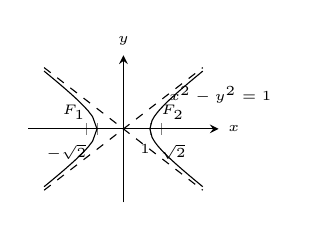
\begin{tikzpicture}[font=\tiny,declare function={f(\x)=sqrt((\x)^2-1);fa(\x)=\x;}]
\pgfmathsetmacro{\f}{sqrt(2)}
\begin{axis}[clip=false,width=4cm,axis lines=middle,xlabel={$x$},ylabel={$y$},xlabel style={at={(current axis.right of origin)},anchor=west},ylabel style={at={(current axis.above origin)},anchor=south},enlargelimits=true,xtick={-\f,\f,1,-1},xticklabels={\llap{$-\sqrt{2}$},\rlap{$\sqrt{2}$},\llap{$1$},},ytick={\empty}]
\addplot[domain=-3:1]{f(x)};
\addplot[domain=-3:1]{-f(x)};
\addplot[domain=1:3]{f(x)}node[pos=0.9,below,xshift=2ex]{$x^2-y^2=1$};
\addplot[domain=1:3]{-f(x)};
\addplot[dashed,domain=-3:3]{fa(x)};
\addplot[dashed,domain=-3:3]{-fa(x)};
\addplot[]plot coordinates {(-\f,0)}node[above,xshift=-1ex]{$F_1$}  {(\f,0)}node[above,xshift=1ex]{$F_2$};
\end{axis}
\end{tikzpicture}
\caption{}
\label{شکل_سوال_مخروط_قطع_زائد_معلومات_الف}
\end{minipage}\hfill
\begin{minipage}{0.22\textwidth}
\begin{tikzpicture}[font=\tiny,declare function={f(\x)=sqrt((\x)^2+8);fa(\x)=\x;}]
\pgfmathsetmacro{\f}{4}
\pgfmathsetmacro{\k}{sqrt(8)}
\begin{axis}[clip=false,width=4cm,axis lines=middle,xlabel={$x$},ylabel={$y$},xlabel style={at={(current axis.right of origin)},anchor=west},ylabel style={at={(current axis.above origin)},anchor=south},enlargelimits=true,ytick={-\f,\f},xtick={\empty}]
\addplot[domain=-4:4]{f(x)}node[above]{$\tfrac{y^2}{8}-\tfrac{x^2}{8}=1$};
\addplot[domain=-4:4]{-f(x)};
\addplot[dashed,domain=-4:4]{fa(x)};
\addplot[dashed,domain=-4:4]{-fa(x)};
\addplot[]plot coordinates {(0,-\f)}node[right]{$F_2$}  {(0,\f)}node[right]{$F_1$};
\end{axis}
\end{tikzpicture}
\caption{}
\label{شکل_سوال_مخروط_قطع_زائد_معلومات_ب}
\end{minipage}\hfill
\begin{minipage}{0.22\textwidth}
\begin{tikzpicture}[font=\tiny,declare function={f(\x)=1/2*sqrt((\x)^2+8);fa(\x)=2*\x;}]
\pgfmathsetmacro{\f}{sqrt(10)}
\pgfmathsetmacro{\k}{sqrt(2)}
\pgfmathsetmacro{\kk}{sqrt(8)}
\begin{axis}[clip=false,width=4cm,axis lines=middle,xlabel={$x$},ylabel={$y$},xlabel style={at={(current axis.right of origin)},anchor=west},ylabel style={at={(current axis.above origin)},anchor=south},enlargelimits=true,xtick={-\f,\f},xticklabels={$-\sqrt{10}$,$\sqrt{10}$},xmax=3,ytick={\empty}]
\addplot[domain=-3:3]({f(x)},x)node[above,xshift={2ex}]{$\tfrac{x^2}{2}-\tfrac{y^2}{8}=1$};
\addplot[domain=-3:3]({-f(x)},x);
\addplot[dashed,domain=-\k:\k]{fa(x)};
\addplot[dashed,domain=-\k:\k]{-fa(x)};
\addplot[]plot coordinates {(-\f,0)}node[above]{$F_1$}  {(\f,0)}node[above]{$F_2$};
\addplot[]plot coordinates {(\k,0)}node[shift={(-1ex,1ex)}]{$\sqrt{2}$};
\end{axis}
\end{tikzpicture}
\caption{}
\label{شکل_سوال_مخروط_قطع_زائد_معلومات_پ}
\end{minipage}\hfill
\begin{minipage}{0.22\textwidth}
\begin{tikzpicture}[font=\tiny,declare function={f(\x)=1/2*sqrt((\x)^2+8);fa(\x)=1/2*\x;}]
\pgfmathsetmacro{\f}{sqrt(10)}
\pgfmathsetmacro{\k}{sqrt(2)}
\pgfmathsetmacro{\kk}{sqrt(8)}
\begin{axis}[clip=false,width=4cm,axis lines=middle,xlabel={$x$},ylabel={$y$},xlabel style={at={(current axis.right of origin)},anchor=west},ylabel style={at={(current axis.above origin)},anchor=south},enlargelimits=true,ytick={-\f,\f},yticklabels={$-\sqrt{10}$,$\sqrt{10}$},ymin=-3,ymax=3,xtick={\empty}]
\addplot[domain=-3:3]{f(x)}node[above,xshift={2ex}]{$\tfrac{y^2}{2}-\tfrac{x^2}{8}=1$};
\addplot[domain=-3:3]{-f(x)};
\addplot[dashed,domain=-3:3]{fa(x)};
\addplot[dashed,domain=-3:3]{-fa(x)};
\addplot[]plot coordinates {(0,-\f)}node[right]{$F_2$}  {(0,\f)}node[right]{$F_1$};
\addplot[]plot coordinates {(0,\k)}node[shift={(-1ex,-1ex)}]{$\sqrt{2}$};
\end{axis}
\end{tikzpicture}
\caption{}
\label{شکل_سوال_مخروط_قطع_زائد_معلومات_ت}
\end{minipage}
\end{figure}
سوال \حوالہ{سوال_مخروط_قطع_زائد_معلومات_سے_مساوات_الف} تا سوال \حوالہ{سوال_مخروط_قطع_زائد_معلومات_سے_مساوات_ب} میں \عددی{xy} مستوی پر پائے جانے والے قطع زائد کے ماسکہ، راس اور متقارب کی معلومات دی گئی ہے۔ قطع زائد کا مرکز \عددی{xy} مستوی کے مبدا پر ہے۔قطع زائد کی معیاری مساوات حاصل کریں۔

\ابتدا{سوال}\شناخت{سوال_مخروط_قطع_زائد_معلومات_سے_مساوات_الف}
ماسکے \عددی{(0,\pm \sqrt{2})} اور متقارب \عددی{y=\pm x}\\
جواب:\quad
$y^2-x^2=1$
\انتہا{سوال}
%========================
\ابتدا{سوال}
ماسکے \عددی{(\pm 2,0)} اور متقارب \عددی{y=\pm\tfrac{1}{\sqrt{3}}x}
\انتہا{سوال}
%========================
\ابتدا{سوال}
راس \عددی{(\pm 3,0)} اور متقارب \عددی{y=\pm\tfrac{4}{3}x}\\
جواب:\quad
$\tfrac{x^2}{9}-\tfrac{y^2}{16}=1$
\انتہا{سوال}
%========================
\ابتدا{سوال}\شناخت{سوال_مخروط_قطع_زائد_معلومات_سے_مساوات_ب}
راس \عددی{(0,\pm 2)} اور متقارب \عددی{y=\pm\tfrac{1}{2}x}
\انتہا{سوال}
%========================
\begin{figure}
\centering
\begin{minipage}{0.22\textwidth}
\begin{tikzpicture}[font=\tiny,declare function={f(\x)=1+1/8*(\x+2)^2;}]
\begin{axis}[clip=false,width=4cm,axis lines=middle,xlabel={$x$},ylabel={$y$},xlabel style={at={(current axis.right of origin)},anchor=west},ylabel style={at={(current axis.above origin)},anchor=south},enlargelimits=true,xtick={1,2,3},ytick={-4,-2,2}]
\addplot[domain=-4:4]({f(x)},x)node[above left]{$(y+2)^2=8(x-1)$};
\addplot[]plot coordinates {(1,-2)}node[circ]{}node[pin=-45:{$V(1,-2)$}]{}  {(3,-2)}node[circ]{}node[right]{$F(3,-2)$};
\end{axis}
\end{tikzpicture}
\caption{}
\label{شکل_سوال_مخروط_ہر_قسم_الف}
\end{minipage}\hfill
\begin{minipage}{0.22\textwidth}
\begin{tikzpicture}[font=\tiny,declare function={fp(\x)=3+3/4*sqrt(16-(\x-4)^2);fn(\x)=3-3/4*sqrt(16-(\x-4)^2);}]
\begin{axis}[clip=false,width=4cm,axis lines=middle,xlabel={$x$},ylabel={$y$},xlabel style={at={(current axis.right of origin)},anchor=west},ylabel style={at={(current axis.above origin)},anchor=south},enlargelimits=true,xtick={4,8},ytick={6}]
\addplot[domain=0.2:8-0.2]{fp(x)}node[pos=0.6,above]{$\tfrac{(x-4)^2}{16}+\tfrac{(y-3)^2}{9}=1$};
\addplot[domain=0.2:8-0.2]{fn(x)};
\addplot[domain=0:0.2]{fp(x)};
\addplot[domain=7.8:8]{fp(x)};
\addplot[domain=0:0.2]{fn(x)};
\addplot[domain=7.8:8]{fn(x)};
\addplot[]plot coordinates {(4-sqrt(7),3)}node[circ]{}node[pin={[pin distance=0.15cm]80:{$F_1(4-\sqrt{7},3)$}}]{};
\addplot[]plot coordinates {(4+sqrt(7),3)}node[circ]{}node[pin={[pin distance=0.15cm]-110:{$F_2(4+\sqrt{7},3)$}}]{};
\addplot[]plot coordinates {(4,3)}node[circ]{}node[above,xshift=2ex]{$C(4,3)$};
\addplot[]plot coordinates {(0,3)}node[circ]{}node[left]{$(0,3)$};
\addplot[]plot coordinates {(8,3)}node[circ]{}node[right]{$(8,3)$};
\end{axis}
\end{tikzpicture}
\caption{}
\label{شکل_سوال_مخروط_ہر_قسم_ب}
\end{minipage}\hfill
\begin{minipage}{0.22\textwidth}
\begin{tikzpicture}[font=\tiny,declare function={fp(\x)=2+4/3*sqrt(9+(\x)^2);fn(\x)=2-4/3*sqrt(9+(\x)^2);fa(\x)=3/4*(\x-2);}]
\pgfmathsetmacro{\k}{5}
\begin{axis}[clip=false,width=4cm,axis lines=middle,xlabel={$x$},ylabel={$y$},xlabel style={at={(current axis.right of origin)},anchor=west},ylabel style={at={(current axis.above origin)},anchor=south},enlargelimits=true,xtick={\empty},ytick={\empty}]
\addplot[domain=-\k:\k]({fp(x)},x)node[above]{$\tfrac{(x-2)^2}{16}-\tfrac{y^2}{9}=1$};
\addplot[domain=-\k:\k]({fn(x)},x);
\addplot[dashed,domain=-5:9]{fa(x)};
\addplot[dashed,domain=-5:9]{-fa(x)}node[pos=0,above,xshift={-1ex}]{$y=-\tfrac{3}{4}(x-2)$};
\addplot[]plot coordinates {(-3,0)}node[circ]{}node[above left]{$(-3,0)$};
\addplot[]plot coordinates {(7,0)}node[circ]{}node[above right]{$(7,0)$};
\addplot[]plot coordinates {(-2,0)}node[circ]{}node[pin=-135:{$(-2,0)$}]{};
\addplot[]plot coordinates {(6,0)}node[circ]{}node[pin=-45:{$(6,0)$}]{};
\end{axis}
\end{tikzpicture}
\caption{}
\label{شکل_سوال_مخروط_ہر_قسم_پ}
\end{minipage}
\end{figure}
%=====================
\موٹا{مخروطی حصوں کا انتقال}\\
\ابتدا{سوال}\شناخت{سوال_مخروط_ہر_قسم_الف}
قطع مکافی \عددی{y^2=8x} کو \عددی{2} اکائیاں نیچے اور \عددی{1} اکائی دائیں منتقل کر کے قطع مکافی  \عددی{(y+2)^2=8(x-1)} پیدا کیا جاتا ہے۔ (الف) نئے قطع مکافی کے راس، ماسکہ اور ناظمہ دریافت کریں۔ (ب) نئے راس، ماسکہ اور ناظمہ کو ترسیم کرتے ہوئے نئے قطع مکافی کا خاکہ بنائیں۔\\
جواب:\quad
(الف) راس \عددی{(1,-2)}، ماسکہ \عددی{(3,-2)}، ناظمہ \عددی{x=-1}؛ (ب) شکل \حوالہ{شکل_سوال_مخروط_ہر_قسم_الف}
\انتہا{سوال}
%====================
\ابتدا{سوال}
قطع مکافی \عددی{x^2=-4y} کو \عددی{1} اکائی بائیں اور \عددی{3} اکائیاں اوپر منتقل کر کے قطع مکافی \عددی{(x+1)^2=-4(y-3)} پیدا کیا جاتا ہے۔   (الف) نئے قطع مکافی کا راس، ماسکہ اور ناظمہ دریافت کریں۔ (ب) نئے راس، ماسکہ اور ناظمہ کو ترسیم کرتے ہوئے نئے قطع مکافی کا خاکہ بنائیں۔
\انتہا{سوال}
%=====================
\ابتدا{سوال}\شناخت{سوال_مخروط_ہر_قسم_ب}
ترخیم \عددی{\tfrac{x^2}{16}+\tfrac{y^2}{9}=1} کو \عددی{4} اکائیاں دائیں اور \عددی{3} اکائیاں اوپر منتقل کر کے ترخیم \عددی{\tfrac{(x-4)^2}{16}+\tfrac{(y-3)^2}{9}=1} پیدا کیا جاتا ہے۔ (الف) نئے ترخیم کے ماسکے، راس اور مرکز دریافت کریں۔ (ب) نئے ماسکے، راس اور مرکز ترسیم کرتے ہوئے نئے ترخیم کا خاکہ بنائیں۔\\
جواب:\quad
(الف) ماسکے \عددی{(4\pm\sqrt{7},3)}، راس \عددی{(8,3)} اور \عددی{(0,3)}، مرکز \عددی{(4,3)}؛ (ب) شکل \حوالہ{شکل_سوال_مخروط_ہر_قسم_ب}
\انتہا{سوال}
%=====================
\ابتدا{سوال}
ترخیم \عددی{\tfrac{x^2}{9}+\tfrac{y^2}{25}=1} کو \عددی{3} اکائیاں بائیں اور \عددی{2} اکائیاں نیچے منتقل کر کے
 ترخیم \عددی{\tfrac{(x+3)^2}{9}+\tfrac{(y+2)^2}{25}=1} پیدا کیا جاتا ہے۔ (الف) نئے ترخیم کے ماسکے، راس اور مرکز دریافت کریں۔ (ب) نئے ماسکے، راس اور مرکز ترسیم کرتے ہوئے نئے ترخیم کا خاکہ بنائیں۔
\انتہا{سوال}
%=====================
\ابتدا{سوال}\شناخت{سوال_مخروط_ہر_قسم_پ}
قطع زائد \عددی{\tfrac{x^2}{16}-\tfrac{y^2}{9}=1} کو \عددی{2} اکائیاں دائیں منتقل کر کے قطع زائد
 \عددی{\tfrac{(x-2)^2}{16}-\tfrac{y^2}{9}=1} پیدا کیا جاتا ہے۔ (الف) نئے قطع زائد کا مرکز، ماسکے، راس اور متقارب دریافت کریں۔ (ب) نئے مرکز، ماسکے، راس اور متقارب ترسیم کرتے ہوئے نئے قطع زائد کا خاکہ بنائیں۔\\
جواب:\quad
(الف) مرکز \عددی{(2,0)}، ماسکے \عددی{(7,0)} اور \عددی{(-3,0)}، راس \عددی{(6,0)} اور \عددی{(-2,0)}،\\
 متقارب \عددی{y=\pm\tfrac{3}{4}(x-2)}؛  (ب) شکل \حوالہ{شکل_سوال_مخروط_ہر_قسم_پ}
\انتہا{سوال}
%======================
\ابتدا{سوال}
قطع زائد \عددی{\tfrac{y^2}{4}-\tfrac{x^2}{5}=1} کو \عددی{2} اکائیاں نیچے منتقل کرتے ہوئے قطع زائد \عددی{\tfrac{(y+2)^2}{4}-\tfrac{x^2}{5}=1} پیدا کیا جاتا ہے۔ (الف) نئے قطع زائد کا مرکز، ماسکے اور متقارب دریافت کریں۔ (ب) نیا مرکز، ماسکے اور متقارب ترسیم کر کے نئے قطع زائد کا خاکہ بنائیں۔
\انتہا{سوال}
%===================

سوال \حوالہ{سوال_مخروط_قطع_مکافی_منتقل_الف} تا سوال \حوالہ{سوال_مخروط_قطع_مکافی_منتقل_ب} میں قطع مکافی کی مساوات اور اس کی منتقلی کی معلومات دی گئی ہے۔ نئے قطع مکافی کی مساوات تلاش کر کے نئے قطع مکافی کا راس، ماسکہ اور ناظمہ معلوم کریں۔

\ابتدا{سوال}\شناخت{سوال_مخروط_قطع_مکافی_منتقل_الف}
\عددی{y^2=4x}، 
\quad
\عددی{2} اکائیاں بائیں اور \عددی{3} اکائیاں  نیچے۔\\
جواب:\quad
\عددی{(y+3)^2=4(x+2)}، راس \عددی{V(-2,-3)}، ماسکہ \عددی{F(-1,-3)}، ناظمہ \عددی{x=-3}
\انتہا{سوال}
%=====================
\ابتدا{سوال}
\عددی{y^2=-12x}، 
\quad
\عددی{4} اکائیاں دائیں اور \عددی{3} اکائیاں  اوپر۔
\انتہا{سوال}
%=====================
\ابتدا{سوال}
\عددی{x^2=8y}، 
\quad
\عددی{1} اکائی دائیں اور \عددی{7} اکائیاں  نیچے۔\\
جواب:\quad
\عددی{(x-1)^2=8(y+7)}، راس \عددی{V(1,-7)}، ماسکہ \عددی{F(1,-5)}، ناظمہ \عددی{y=-9}
\انتہا{سوال}
%=====================
\ابتدا{سوال}\شناخت{سوال_مخروط_قطع_مکافی_منتقل_ب}
\عددی{x^2=6y}، 
\quad
\عددی{3} اکائیاں بائیں اور \عددی{2} اکائیاں  نیچے۔
\انتہا{سوال}
%=====================

سوال \حوالہ{سوال_مخروط_ترخیم_منتقل_الف} تا سوال \حوالہ{سوال_مخروط_ترخیم_منتقل_ب} میں ترخیم کی مساوات اور اس کی منتقلی کی معلومات دی گئی ہے۔ نئے ترخیم کی مساوات تلاش کر کے نئے ترخیم کے ماسکے، راس اور مرکز معلوم کریں۔

\ابتدا{سوال}\شناخت{سوال_مخروط_ترخیم_منتقل_الف}
\عددی{\tfrac{x^2}{6}+\tfrac{y^2}{9}=1}، 
\quad
\عددی{2} اکائیاں بائیں اور \عددی{1} اکائی نیچے۔\\
جواب:\quad
\عددی{\tfrac{(x+2)^2}{6}+\tfrac{(y+1)^2}{9}=1}، \عددی{F(-2,\pm\sqrt{3}-1)}، \عددی{V(-2,\pm 3-1)}، \عددی{C(-2,-1)}
\انتہا{سوال}
%=====================
\ابتدا{سوال}
\عددی{\tfrac{x^2}{2}+y^2=1}، 
\quad
\عددی{3} اکائیاں دائیں اور \عددی{4} اکائیاں اوپر۔
\انتہا{سوال}
%=====================
\ابتدا{سوال}
\عددی{\tfrac{x^2}{3}+\tfrac{y^2}{2}=1}، 
\quad
\عددی{2} اکائیاں دائیں اور \عددی{3} اکائیاں اوپر۔\\
جواب:\quad
\عددی{\tfrac{(x-2)^2}{3}+\tfrac{(y-3)^2}{2}=1}، \عددی{F(3,3)} اور \عددی{F(1,3)}، \عددی{V(\pm\sqrt{3}+2,3)}، \عددی{C(2,3)}
\انتہا{سوال}
%=====================
\ابتدا{سوال}\شناخت{سوال_مخروط_ترخیم_منتقل_ب}
\عددی{\tfrac{x^2}{16}+\tfrac{y^2}{25}=1}، 
\quad
\عددی{43} اکائیاں بائیں اور \عددی{5} اکائیاں نیچے۔
\انتہا{سوال}
%=====================


سوال \حوالہ{سوال_مخروط_قطع_زائد_منتقل_الف} تا سوال \حوالہ{سوال_مخروط_قطع_زائد_منتقل_ب} میں قطع زائد کی مساوات اور اس کی منتقلی کی معلومات دی گئی ہے۔ نئے قطع زائد کی مساوات تلاش کر کے نئے قطع زائد کا مرکز، ماسکے، راس اور متقارب معلوم کریں۔

\ابتدا{سوال}\شناخت{سوال_مخروط_قطع_زائد_منتقل_الف}
$\tfrac{x^2}{4}-\tfrac{y^2}{5}=1$\quad
دائیں \عددی{2} اکائیاں اور اوپر \عددی{2} اکائیاں۔\\
جواب:\quad
\عددی{\tfrac{(x-2)^2}{4}-\tfrac{(y-2)^2}{5}=1}، \عددی{C(2,2)}، \عددی{F(5,2)} اور \عددی{F(-1,2)}، \عددی{V(4,2)} اور \عددی{V(0,2)}، متقارب \عددی{y-2=\pm\tfrac{\sqrt{5}}{2}(x-2)}
\انتہا{سوال}
%=======================
\ابتدا{سوال}
$\tfrac{x^2}{16}-\tfrac{y^2}{9}=1$\quad
بائیں \عددی{5} اکائیاں اور نیچے \عددی{1} اکائی۔
\انتہا{سوال}
%=======================
\ابتدا{سوال}
$y^2-x^2=1$\quad
بائیں \عددی{1} اکائی اور نیچے \عددی{1} اکائی۔\\
جواب:\quad
\عددی{(y+1)^2-(x+1)^2=1}، \عددی{C(-1,-1)}، \عددی{F(-1,\sqrt{2}-1)} اور \عددی{F(-1,-\sqrt{2}-1)}، \عددی{V(-1,0)}، \عددی{V(-1,-2)}، متقارب \عددی{y+1=\pm(x+1)}
\انتہا{سوال}
%=======================
\ابتدا{سوال}\شناخت{سوال_مخروط_قطع_زائد_منتقل_ب}
$\tfrac{y^2}{3}-x^2=1$\quad
دائیں \عددی{1} اکائی اور اوپر \عددی{3} اکائیاں۔
\انتہا{سوال}
%=======================

سوال \حوالہ{سوال_مخروط_مساوات_منتقلی_الف} تا سوال \حوالہ{سوال_مخروط_مساوات_منتقلی_ب} میں دیے گئے مخروط حصوں کا (جیسا مناسب ہو) مرکز، ماسکے، راس، متقارب اور رداس دریافت کریں۔

\ابتدا{سوال}\شناخت{سوال_مخروط_مساوات_منتقلی_الف}
$x^2+4x+y^2=12$\\
جواب:\quad 
\عددی{C(-2,0)}، \عددی{a=4}
\انتہا{سوال}
%====================
\ابتدا{سوال}
$2x^2+2y^2-28x+12y+144$
\انتہا{سوال}
%====================
\ابتدا{سوال}
$x^2+2x+4y-3=0$\\
جواب:\quad
\عددی{V(-1,1)}، \عددی{F(-1,0)}
\انتہا{سوال}
%====================
\ابتدا{سوال}
$y^2-4y-8x-12=0$
\انتہا{سوال}
%====================
\ابتدا{سوال}
$x^2+5y^2+4x=1$\\
جواب:\quad
ترخیم \عددی{\tfrac{(x+2)^2}{5}+y^2=1}، \عددی{C(-2,0)}، \عددی{F(0,0)} اور \عددی{F(-4,0)}، \عددی{V(\sqrt{5}-2,0)} اور \عددی{V(-\sqrt{5}-2,0)}
\انتہا{سوال}
%====================
\ابتدا{سوال}
$9x^2+6y^2+36y=0$
\انتہا{سوال}
%====================
\ابتدا{سوال}
$x^2+2y^2-2x-4y=-1$\\
جواب:\quad
ترخیم \عددی{\tfrac{(x-1)^2}{5}+(y-1)^2=1}، \عددی{C(1,1)}، \عددی{F(2,1)} اور \عددی{F(0,1)}، \عددی{V(\sqrt{2}+1,1)} اور 
\عددی{V(-\sqrt{2}+1,1)}
\انتہا{سوال}
%====================
\ابتدا{سوال}
$4x^2+y^2+8x-2y=-1$
\انتہا{سوال}
%====================
\ابتدا{سوال}
$x^2-y^2-2x+4y=4$\\
جواب:\quad
قطع زائد \عددی{(x-1)^2-(y-2)^2=1}، \عددی{C(1,2)}، \عددی{F(1+\sqrt{2},2)} اور \عددی{F(1-\sqrt{2},2)}، \عددی{V(2,2)} اور \عددی{V(0,2)}، متقارب \عددی{y-2=\pm(x-1)}
\انتہا{سوال}
%====================
\ابتدا{سوال}
$x^2-y^2+4x-6y=6$
\انتہا{سوال}
%====================
\ابتدا{سوال}
$2x^2-y^2+6y=3$\\
جواب:\quad
قطع زائد، \عددی{\tfrac{(y-3)^2}{6}-\tfrac{x^2}{3}=1}، \عددی{C(0,3)}، \عددی{F(0,6)} اور \عددی{F(0,0)}، \عددی{V(0,\sqrt{6}+3)} اور \عددی{V(0,-\sqrt{6}+3)}، متقارب \عددی{y=\sqrt{2}x+3} اور \عددی{y=-\sqrt{2}x+3}
\انتہا{سوال}
%====================
\ابتدا{سوال}\شناخت{سوال_مخروط_مساوات_منتقلی_ب}
$y^2-4x^2+16x=24$
\انتہا{سوال}
%====================

\موٹا{عدم مساوات}\\
سوال \حوالہ{سوال_مخروط_خطے_الف} تا سوال \حوالہ{سوال_مخروط_خطے_ت} میں ایک خطہ کو مطمئن کرنے والی  عدم مساوات یا عدم مساوات کی جوڑی  دی گئی ہے۔ \عددی{xy} مستوی میں اس خطہ کو ترسیم کریں۔

\ابتدا{سوال}\شناخت{سوال_مخروط_خطے_الف}
$9x^2+16y^2\le 144$\\
جواب:\quad
ترسیم شکل \حوالہ{شکل_سوال_مخروط_خطے_الف} میں دی گئی ہے۔
\انتہا{سوال}
%========================
\ابتدا{سوال}
$x^2+y^2\ge 1\quad\text{اور}\quad  4x^2+y^2\le 4$
\انتہا{سوال}
%========================
\ابتدا{سوال}\شناخت{سوال_مخروط_خطے_ب}
$x^2+4y^2\ge 4\quad\text{اور}\quad 4x^2+9y^2\le 36$\\
جواب:\quad
ترسیم شکل \حوالہ{شکل_سوال_مخروط_خطے_ب} میں دی گئی ہے۔
\انتہا{سوال}
%========================
\ابتدا{سوال}
$(x^2+y^2-4)(x^2+9y^2-9)\le 0$
\انتہا{سوال}
%========================
\ابتدا{سوال}\شناخت{سوال_مخروط_خطے_پ}
$4y^2-x^2\ge 4$\\
جواب:\quad
ترسیم شکل \حوالہ{شکل_سوال_مخروط_خطے_پ} میں دی گئی ہے۔
\انتہا{سوال}
%========================
\ابتدا{سوال}\شناخت{سوال_مخروط_خطے_ت}
$\abs{x^2-y^2}\le 1$
\انتہا{سوال}
%========================
%========================
\begin{figure}
\centering
\begin{minipage}{0.22\textwidth}
\centering
\begin{tikzpicture}[font=\tiny,declare function={f(\x)=1/4*sqrt(144-9*(\x)^2);}]
\begin{axis}[axis on top=true,clip=false,width=4cm,axis lines=middle,xlabel={$x$},ylabel={$y$},xlabel style={at={(current axis.right of origin)},anchor=west},ylabel style={at={(current axis.above origin)},anchor=south},enlargelimits=true,xtick={4},ytick={3}]
\addplot[name path=a,domain=-4+0.2:4-0.2]{f(x)}node[pos=0.75,above right]{$9x^2+16y^2\le 144$};
\addplot[name path=aa,domain=-4+0.2:4-0.2]{-f(x)};
\addplot[name path=b,domain=-4:-4+0.2]{f(x)};
\addplot[name path=c,domain=4-0.2:4]{f(x)};
\addplot[name path=bb,domain=-4:-4+0.2]{-f(x)};
\addplot[name path=cc,domain=4-0.2:4]{-f(x)};
\addplot[llgray] fill between [of={a and aa}];
\addplot[llgray] fill between [of={b and bb}];
\addplot[llgray] fill between [of={c and cc}];
\end{axis}
\end{tikzpicture}
\caption{}
\label{شکل_سوال_مخروط_خطے_الف}
\end{minipage}\hfill
\begin{minipage}{0.22\textwidth}
\centering
\begin{tikzpicture}[font=\tiny,declare function={fa(\x)=1/4*sqrt(4-(\x)^2);fb(\x)=1/3*sqrt(36-4*(\x)^2);}]
\pgfmathsetmacro{\k}{2}
\pgfmathsetmacro{\kk}{3}
\begin{axis}[axis on top=true,clip=false,width=4cm,axis lines=middle,xlabel={$x$},ylabel={$y$},xlabel style={at={(current axis.right of origin)},anchor=west},ylabel style={at={(current axis.above origin)},anchor=south},enlargelimits=true,xtick={3},ytick={3}]
\addplot[name path=a,domain=-\kk+0.2:\kk-0.2]{fb(x)}node[pos=0.75,above right]{$4x^2+9y^2\le 36$}node[pos=0.25,above left]{$x^2+4y^2\ge 4$};
\addplot[name path=aa,domain=-\kk+0.2:\kk-0.2]{-fb(x)};
\addplot[name path=b,domain=-\kk:-\kk+0.2]{fb(x)};
\addplot[name path=c,domain=\kk-0.2:\kk]{fb(x)};
\addplot[name path=bb,domain=-\kk:-\kk+0.2]{-fb(x)};
\addplot[name path=cc,domain=\kk-0.2:\kk]{-fb(x)};
\addplot[llgray] fill between [of={a and aa}];
\addplot[llgray] fill between [of={b and bb}];
\addplot[llgray] fill between [of={c and cc}];
\addplot[name path=a,domain=-\k+0.2:\k-0.2]{fa(x)};
\addplot[name path=aa,domain=-\k+0.2:\k-0.2]{-fa(x)};
\addplot[name path=b,domain=-\k:-\k+0.2]{fa(x)};
\addplot[name path=c,domain=\k-0.2:\k]{fa(x)};
\addplot[name path=bb,domain=-\k:-\k+0.2]{-fa(x)};
\addplot[name path=cc,domain=\k-0.2:\k]{-fa(x)};
\addplot[white] fill between [of={a and aa}];
\addplot[white] fill between [of={b and bb}];
\addplot[white] fill between [of={c and cc}];
\end{axis}
\end{tikzpicture}
\caption{}
\label{شکل_سوال_مخروط_خطے_ب}
\end{minipage}\hfill
\begin{minipage}{0.22\textwidth}
\centering
\begin{tikzpicture}[font=\tiny,declare function={f(\x)=1/2*sqrt(4+(\x)^2);}]
\begin{axis}[axis on top=true,clip=false,width=4cm,axis lines=middle,xlabel={$x$},ylabel={$y$},xlabel style={at={(current axis.right of origin)},anchor=west},ylabel style={at={(current axis.above origin)},anchor=south},enlargelimits=true]
\addplot[name path=a,domain=-4:4]{f(x)}node[pos=0.85,below]{$4y^2-x^2\ge 4$};
\addplot[name path=aa,domain=-4:4]{-f(x)};
\addplot[name path=t,draw=none] plot coordinates {(-4,3)(4,3)};
\addplot[name path=b,draw=none] plot coordinates {(-4,-3)(4,-3)};
\addplot[llgray] fill between [of={t and b}];
\addplot[white] fill between [of={a and aa}];
\end{axis}
\end{tikzpicture}
\caption{}
\label{شکل_سوال_مخروط_خطے_پ}
\end{minipage}
\end{figure}

\موٹا{نظریہ اور مثالیں}

\ابتدا{سوال}\شناخت{سوال_مخروط_قطع_مکافی_حجم}\ترچھا{قطع مکافی ٹھوس جسم کے حجم کا کلیہ آرشمیدسی }\\
قطع مکافی \عددی{y=\tfrac{4h}{b^2}x^2} اور لکیر \عددی{y=h} میں  گھیرے ہوئے خطے کو \عددی{y} محور کے گرد گھما کر جسم طواف پیدا کیا جاتا ہے۔ دکھائیں کہ اس جسم کا حجم مطابقتی مخروط کے حجم کا\عددی{\tfrac{3}{2}} گنّا ہو گا (شکل \حوالہ{شکل_سوال_مخروط_قطع_مکافی_حجم})۔ 
\انتہا{سوال}
%=======================


\begin{figure}
\centering
\begin{minipage}{0.45\textwidth}
\centering
\begin{tikzpicture}[yscale=0.75,declare function={f(\x)=\x^2;}]
\draw[-latex](0,0)--(2.5,0)node[right]{$x$};
\draw[-latex](0,{f(2)})--++(0,0.75)node[above]{$y$};
\draw[thick,domain=0:2]plot ({\x},{f(\x)});
\draw[domain=0:2]plot ({-\x},{f(\x)});
\draw (0,4)circle (2cm and 0.25cm);
\draw(-2,4)--(0,0)--(2,4)coordinate[pos=0.5](ka);
\draw(ka)node[pin={[pin distance=1cm]30:{مخروط}}]{};
\draw(1.25,{f(1.25)})node[right]{$y=\frac{4h}{b^2}x^2$};
\draw(2,{f(2)})node[right]{$(\tfrac{b}{2},h)$};
\end{tikzpicture}
\caption{جسم طواف برائے سوال \حوالہ{سوال_مخروط_قطع_مکافی_حجم}}
\label{شکل_سوال_مخروط_قطع_مکافی_حجم}
\end{minipage}\hfill
\begin{minipage}{0.45\textwidth}
\centering
\begin{tikzpicture}[declare function={f(\x)=sqrt(\x);}]
\begin{axis}[clip=false,small, axis lines=middle,xtick={\empty},ytick={\empty},xlabel={$x$},ylabel={$y$},xlabel style={at={(current axis.right of origin)},anchor=west},ylabel={$y$},ylabel style={at={(current axis.above origin)},anchor=south},enlargelimits=true]
\addplot[domain=0:0.5]{f(x)};
\addplot[domain=0.5:4]{f(x)}node[pos=0.5,below right]{$y^2=kx$};
\addplot[]plot coordinates {(3.75,{f(3.75)})}node[circ]{}node[below right]{$N$};
\addplot[]plot coordinates {(3.75,{f(3.75)})(3.75,0)};
\addplot[]plot coordinates {(3.75,{f(3.75)})(0,{f(3.75)})};
\addplot[]plot coordinates {(2,0.75)}node[]{$B$}  {(1,1.5)}node[]{$A$};
\end{axis}
\end{tikzpicture}
\caption{خطے برائے سوال \حوالہ{سوال_مخلوط_قطع_مکافی_خطے}}
\label{شکل_سوال_مخلوط_قطع_مکافی_خطے}
\end{minipage}
\end{figure}

\ابتدا{سوال}\ترچھا{معلق پل کی رسیاں قطع مکافی کی صورت میں لٹکی ہوتی ہیں۔}\\
ایک معلق پل کی کمیت \عددی{m} کلو گرام فی میٹر ہے۔ اس پل کو رسیوں سے لٹکایا گیا ہے۔ اگر مبدا پر رسی کا افقی تناو \عددی{H} ہو تب رسی کی منحنی درج ذیل مساوات کو مطمئن کرتی ہے جہاں \عددی{g=\SI{9.8}{\meter\per\second\squared}} ہے۔
\begin{align*}
\frac{\dif y}{\dif x}=\frac{mg}{H}x
\end{align*}
اس تفرقی مساوات کو حل کرتے ہوئے دکھائیں کہ رسی کی منحنی کی مساوات ایک قطع مکافی ہے۔ \عددی{x=0} پر \عددی{y=0} ابتدائی معلومات ہے۔
\انتہا{سوال}
%========================
\ابتدا{سوال}
نقاط \عددی{(1,0)}، \عددی{(0,1)} اور \عددی{(2,2)} سے گزرتے دائرے کی مساوات دریافت کریں۔\\
جواب:\quad
$3x^2+3y^2-7x-7y+4=0$
\انتہا{سوال}
%=======================
\ابتدا{سوال}
نقاط \عددی{(2,3)}، \عددی{(3,2)} اور \عددی{(-4,3)} سے گزرتے دائرے کی مساوات دریافت کریں۔
\انتہا{سوال}
%=======================
\ابتدا{سوال}
ایک دائرہ جس کا مرکز \عددی{(-2,1)} پر ہے نقطہ \عددی{(1,3)} سے گزرتا ہے۔  کیا نقطہ \عددی{(1.1,2.8)} اس دائرے پر، اس کے اندر یا اس کے باہر پایا جاتا ہے؟\\
جواب:\quad
$(x+2)^2+(y-1)^2=13$\quad
نقطہ دائرے کے اندر ہے۔ 
\انتہا{سوال}
%====================
\ابتدا{سوال}
جہاں دائرہ \عددی{(x-2)^2+(y-1)^2=5} محددی محوروں کو قطع کرتا ہے وہاں اس دائرے کے مماس معلوم کریں۔ 
\انتہا{سوال}
%===================
\ابتدا{سوال}\شناخت{سوال_مخلوط_قطع_مکافی_خطے}
قطع مکافی \عددی{y^2=kx,\, k>0} پر نقطہ \عددی{N} سے محددی محور کے متوازی لکیریں کھینچی جاتی ہیں۔ ان لکیروں اور محددی محوروں کے کے بیچ مستطیل خطہ کو قطع مکافی دو حصوں \عددی{A} اور \عددی{B} میں تقسیم کرتا ہے (شکل \حوالہ{شکل_سوال_مخلوط_قطع_مکافی_خطے})۔ (الف) دکھائیں کہ ان خطوں کو \عددی{y} محور کے گرد گھما کر حاصل اجسام طواف کے حجم کی نسبت \عددی{4:1} ہے۔ (ب) ان خطوں کو \عددی{x} محور کے گرد گھما کر حاصل اجسام طواف کے حجم کی نسبت کیا ہو گی؟\\
جواب:\quad
(ب)\عددی{1:1}
\انتہا{سوال}
%===================
\ابتدا{سوال}
دکھائیں کہ لکیر \عددی{x=-p} پر  کسی بھی نقطہ سے منحنی \عددی{y^2=4px} پر دو مماس، آپس میں عمودی ہوں گے۔  
\انتہا{سوال}
%=================
\ابتدا{سوال}
ترخیم \عددی{x^2+4y^2=4} میں محصور زیادہ سے زیادہ رقبے کے مستطیل کے اضلاع معلوم کریں۔مستطیل کے اضلاع محددی محور کے متوازی ہیں۔ \\
جواب:\quad
لمبائی \عددی{2\sqrt{2}}، چوڑائی \عددی{\sqrt{2}}، رقبہ \عددی{4}
\انتہا{سوال}
%====================
\ابتدا{سوال}
ترخیم \عددی{9x^2+4y^2=36} کو (الف) \عددی{x} محور، (ب) \عددی{y} محور کے گرد گھما کر جسم طواف پیدا کیا جاتا ہے۔ اس کا حجم معلوم کریں۔
\انتہا{سوال}
%=====================
\ابتدا{سوال}
ربع اول میں \عددی{x} محور، لکیر \عددی{x=4} اور قطع زائد \عددی{9x^2-4y^2=36} کے بیچ تکونی خطہ کو \عددی{x} محور کے گرد گھما کر جسم طواف پیدا کیا جاتا ہے۔  اس جسم کا حجم تلاش کریں۔\\
جواب:\quad
\عددی{24\pi}
\انتہا{سوال}
%====================
\ابتدا{سوال}
ایک خطہ کا بایاں سرحد محور \عددی{y}، دایاں سرحد قطع زائد \عددی{x^2-y^2=1}  جبکہ اس کا نچلا اور بالائی سرحد لکیر \عددی{y=\pm 3} ہیں۔ اس خطہ کو \عددی{y} محور کے گرد گھما کر جسم طواف پیدا کیا جاتا ہے۔ اس جسم کا حجم تلاش کریں۔ 
\انتہا{سوال}
%=======================
\ابتدا{سوال}
محور \عددی{x} کے بالائی اور ترخیم \عددی{\tfrac{x^2}{9}+\tfrac{y^2}{16}=1} کے نیچے  خطے کا وسطانی مرکز تلاش کریں۔\\
جواب:\quad
\عددی{(0,\tfrac{16}{3\pi})}
\انتہا{سوال}
%================
\ابتدا{سوال}
قطع زائد \عددی{y^2-x^2=1} کے بالائی شاخ \عددی{y=\sqrt{x^2+1},\, 0\le x\le \sqrt{2}} کو \عددی{x} محور کر گرد گھما کر سطح طواف پیدا کیا جاتا ہے۔ اس سطح کا رقبہ تلاش کریں۔
\انتہا{سوال}
%==================
\ابتدا{سوال}\شناخت{سوال_مخروط_امواج}
پانی کی سطح کو پہلے \عددی{A} اور بعد میں \عددی{B} پر چھو کر شکل \حوالہ{شکل_سوال_مخروط_امواج} میں دکھائے گئے امواج پیدا کئے گئے۔ جیسے جیسے یہ امواج پھیلتے ہیں، ان کا نقطہ قطع ایک منحنی بناتا ہے جو قطع زائد کی طرح معلوم ہوتا ہے۔ کیا ایسا حقیقتاً ہو گا؟  یہ جاننے کے کئے ہم \عددی{A} اور \عددی{B} پر مرکز دائروں کو امواج کا نمونہ لے سکتے ہیں۔

لمحہ \عددی{t} پر نقطہ \عددی{N} مرکز \عددی{A} سے \عددی{r_A(t)}  اور \عددی{B} سے \عددی{r_B(t)} فاصلہ پر ہو گا۔ چونکہ دائروں کے رداس ایک مستقل رفتار (موج کی رفتار) سے بڑھتے ہیں لہٰذا \عددی{\tfrac{\dif r_A}{\dif t}=\tfrac{\dif r_B}{\dif t}} ہو گا۔ اس سے اخذ کریں کہ
 \عددی{r_A-r_B} ایک مستقل ہو گا لہٰذا \عددی{N} اس قطع زائد پر پایا جائے گا جس کے ماسکہ \عددی{A} اور \عددی{B} ہیں۔
\انتہا{سوال}
%============
\begin{figure}
\centering
\begin{minipage}{0.45\textwidth}
\centering
\begin{tikzpicture}
\draw[name path=a] (0,0)node[circ]{}node[below]{$A$} circle (1.5);
\draw[name path=b] (0.75,0)node[circ]{}node[below]{$B$} circle (1.25);
\draw[name intersections={of={a and b}}](0,0)--(intersection-1)node[circ]{}node[above]{$N(t)$}node[pos=0.5,shift={(-1ex,1ex)},font=\scriptsize]{$r_A(t)$};
\draw(0.75,0)--(intersection-1)node[pos=0.4,xshift=1ex,,fill=white,font=\scriptsize]{$r_B(t)$};
\end{tikzpicture}
\caption{امواج برائے سوال \حوالہ{سوال_مخروط_امواج}}
\label{شکل_سوال_مخروط_امواج}
\end{minipage}\hfill
\begin{minipage}{0.45\textwidth}
\centering
\begin{tikzpicture}[font=\scriptsize,declare function={f(\x)=sqrt(\x);ft(\x)=1/2*(\x+1);}]
\pgfmathsetmacro{\B}{atan(0.5)}
\pgfmathsetmacro{\P}{atan(1/0.75)}
\pgfmathsetmacro{\D}{\P-\B}
\draw[-latex](0,0)--(2,0)node[right]{$x$};
\draw[-latex](0,0)--(0,1.5)node[above]{$y$};
\draw[domain=0:2]plot (\x,{ft(\x)});
\draw[domain=0.2:2]plot (\x,{f(\x)});
\draw[domain=0:0.2]plot(\x,{f(\x)});
\draw[domain=0:0.2]plot(\x,{-f(\x)});
\draw[domain=0.2:2]plot (\x,{-f(\x)});
\draw[]plot coordinates {(0.25,0)(1,{f(1)})};
\draw[]plot coordinates {(0,{f(1)})(2,{f(1)})}node[right]{$L'$};
\draw([shift={(0:0.7)}]1,1) arc (0:\B:0.7);
\draw(1,1)++(0.9,0.15)node[]{$\beta$};
\draw(1.75,{-f(1.25)})node[above]{$y^2=4px$};
\draw(0.25,0)node[circ]{}node[below,xshift=2ex]{$F(p,0)$};
\draw(1,1)node[above,xshift=-2ex]{$N(x_0,y_0)$};
\draw(2,{ft(2)})node[above]{$L$};
\draw(1,1)--(1,0)node[pos=0.5,right]{$y_0$};
\draw([shift={(0:0.3)}]0.25,0) arc (0:\P:0.3);
\draw(20:0.7)node[]{$\phi$};
\draw([shift={(180:0.5)}]1,1) arc (180:180+\D:0.5);
\draw(1,1)++(-0.6,-0.15)node[]{$\beta$};
\draw([shift={(180+\B:0.7)}]1,1) arc (180+\B:180+2*\B:0.7);
\draw(1,1)++(-0.6,-0.6)node[]{$\alpha$};
\end{tikzpicture}
\caption{قطع مکافی میں انعکاس (سوال \حوالہ{سوال_مخروط_قطع_مکافی_انعکاس})}
\label{شکل_سوال_مخروط_قطع_مکافی_انعکاس}
\end{minipage}
\end{figure}


\ابتدا{سوال}\شناخت{سوال_مخروط_قطع_مکافی_انعکاس}\ترچھا{قطع مکافی کے خواص انعکاس}\\
قطع مکافی \عددی{y^2=4px} پر عمومی نقطہ \عددی{N(x_0,y_0)} کو شکل \حوالہ{شکل_سوال_مخروط_قطع_مکافی_انعکاس} میں دکھایا گیا ہے۔ نقطہ \عددی{N} پر لکیر \عددی{L} اس قطع مکافی کا مماس ہے۔ قطع مکافی کا ماسکہ \عددی{F(p,0)} ہے۔نقطہ \عددی{N} سے دائیں منعکس شعاع \عددی{L'}، محور \عددی{x} کے متوازی  ہے۔ ہم دکھاتے ہیں کہ \عددی{F} سے خارج، \عددی{N} پر پہنچتا شعاع انعکاس کے بعد \عددی{L'} کا ہم مکان ہو گا۔ یہ دکھانے کی خاطر ہم دکھاتے ہیں کہ \عددی{\beta=\alpha} ہو گا۔ اس مساوات کی تصدیق درج ذیل اقدام کے ذریعہ کریں۔
\begin{enumerate}[a.]
\item
دکھائیں کہ \عددی{\tan \beta=\tfrac{2p}{y_0}} ہو گا۔
\item
دکھائیں کہ \عددی{\tan \phi=\tfrac{y_0}{x_0-p}} ہو گا۔
\item
درج ذیل مماثل
\begin{align*}
\tan \alpha=\frac{\tan \phi-\tan\beta}{1+\tan\phi\tan\beta}
\end{align*}
استعمال کرتے ہوئے دکھائیں کہ \عددی{\tan\alpha=\tfrac{2p}{y_0}} ہو گا۔چونکہ \عددی{\alpha} اور \عددی{\beta} دونوں زاویہ حادہ ہیں لہٰذا
 \عددی{\tan\beta=\tan\alpha} یعنی \عددی{\beta=\alpha} ہو گا۔ 
\end{enumerate}  
\انتہا{سوال}
%======================

\حصہ{سنک لے لحاظ سے مخروط حصوں کی جماعت بندی}ہم ہر مخروط حصہ کے ساتھ ایک عدد منسلک کر سکتے ہیں جس کو مخروط حصے کا سنک کہتے ہیں۔ سنک سے مخروط حصے کی قسم (دائرہ، ترخیم، قطع مکافی یا قطع زائد) معلوم کی جا سکتی ہے۔ ترخیم اور قطع زائد کی صورت میں یہ عدد مخروط کی عمومی جسامت کی معلومات بھی فراہم کرتا ہے۔

\جزوحصہء{سنک}
اگرچہ مرکز سے ماسکہ تک فاصلہ \عددی{c} درج ذیل مساوات میں نہیں پایا جاتا ہے
\begin{align*}
\frac{x^2}{a^2}+\frac{y^2}{b^2}=1\quad (a>b)
\end{align*}
ترخیم کے لئے ہم \عددی{c} کو \عددی{c=\sqrt{a^2-b^2}} سے معلوم کر سکتے ہیں۔ اگر \عددی{a} کو مستقل رکھ کر \عددی{c} کو وقفہ \عددی{0\le c\le a} پر تبدیل کیا جائے تب حاصل ترخیم کی صورت  بھی تبدیل ہو گی (شکل \حوالہ{شکل_مخروط_تبدیلی_صورت_ترخیم})۔ اگر \عددی{c=0} (یعنی \عددی{a=b}) ہو تب یہ دائرہ ہو گا جبکہ \عددی{c} بڑھانے سے یہ چپٹا ہو گا۔ اگر \عددی{c=a} ہو تب راس اور ماسکے ایک دوسرے کے اوپر ہوں گے اور ترخیم ایک سیدھی لکیر کی صورت اختیار کرے گا۔

ہم \عددی{c} اور \عددی{a} کی نسبت سے ترخیم کی صورت بیان کرتے ہیں۔ یہ نسبت ترخیم کی \اصطلاح{سنک} کہلاتی ہے۔
\begin{figure}
\centering
\begin{subfigure}{0.3\textwidth}
\centering
\begin{tikzpicture}
\draw(-2,0)--(2,0);
\draw(0,0)node[circ]{}node[below]{$F_1=F_2$} circle (1.5cm);
\draw(1.5,0)node[circ]{}  (-1.5,0)node[circ]{};
\draw(0,0.5)node[left,xshift=-2ex]{$c=0$}node[right,xshift=2ex]{$e=0$};
\end{tikzpicture}
\end{subfigure}\hfill
\begin{subfigure}{0.3\textwidth}
\centering
\begin{tikzpicture}
\pgfmathsetmacro{\a}{1.5}
\pgfmathsetmacro{\b}{3/5*\a}
\pgfmathsetmacro{\c}{sqrt(\a^2-\b^2)}
\draw(-2,0)--(2,0);
\draw(0,0)node[circ]{} circle (\a cm and \b cm);
\draw(-\c,0)node[circ]{}node[below]{$F_1$};
\draw(\c,0)node[circ]{}node[below,xshift={-0.25ex}]{$F_2$};
\draw(1.5,0)node[circ]{}  (-1.5,0)node[circ]{};
\draw(0,0.4)node[left,xshift=-0.5ex]{$c=\tfrac{4a}{5}$}node[right,xshift=0.5ex]{$e=\tfrac{4}{5}$};
\end{tikzpicture}
\end{subfigure}\hfill
\begin{subfigure}{0.3\textwidth}
\centering
\begin{tikzpicture}
\pgfmathsetmacro{\a}{1.5}
\pgfmathsetmacro{\b}{3/5*\a}
\pgfmathsetmacro{\c}{sqrt(\a^2-\b^2)}
\draw(-2,0)--(2,0);
\draw(0,0)node[circ]{};
\draw(-\a,0)node[circ]{}node[below]{$F_1$};
\draw(\a,0)node[circ]{}node[below,xshift={-0.25ex}]{$F_2$};
\draw(1.5,0)node[circ]{}  (-1.5,0)node[circ]{};
\draw(0,0.4)node[left,xshift=-0.5ex]{$c=a$}node[right,xshift=0.5ex]{$e=1$};
\end{tikzpicture}
\end{subfigure}
\caption{اگر \عددی{c} کو \عددی{0} سے بڑھا کر \عددی{a} کیا جائے تب ترخیم کی صورت دائرہ سے لکیر کی ہو جاتی ہے۔}
\label{شکل_مخروط_تبدیلی_صورت_ترخیم}
\end{figure}

\ابتدا{تعریف}
ترخیم \عددی{\tfrac{x^2}{a^2}+\tfrac{y^2}{b^2}=1,\,\, (a>b)} کی \اصطلاح{سنک}\فرہنگ{سنک}\حاشیہب{eccentricity}\فرہنگ{eccentricity} درج ذیل ہے۔
\begin{align*}
e=\frac{c}{a}=\frac{\sqrt{a^2-b^2}}{a}
\end{align*}
\انتہا{تعریف}
%==========

نظام شمسی میں سورج کے گرد سیاروں کا مدار ترخیمی ہے۔  جیسا جدول \حوالہ{جدول_مخروط_سنک} میں ان مدار کی سنک سے دیکھا جا سکتا ہے  یہ زیادہ تر تقریباً دائری ہیں۔ پلوٹو کا مدار بہت سنکی ہے اور اس  کی سنک \عددی{e=0.21} ہے۔اسی طرح عطارہ کی سنک \عددی{0.21} ہے۔ نظام شمسی کے دیگر ارکان کے مدار مزید زیادہ سنکی ہیں۔مثال کے طور پر سیارچہ آئکارس  جو تقریباً \عددی{1.4} کلومیٹر چوڑا  اور سورج کے گرد \عددی{409} زمینی دنوں میں ایک چکر کاٹتا ہے کی سنک \عددی{0.83} ہے۔

\begin{table}
\caption{سورج کے گرد سیاروں کے مداروں کی سنک}
\label{جدول_مخروط_سنک}
\centering
\begin{tabular}{lllllllll}
\toprule
عطارہ&زھرہ&زمین&مریخ&مشتری&زحل&یورانس&نیپچون&پلوٹو\\
 $0.21$&$0.01$&$0.02$&$0.09$&$0.05$&$0.06$&$0.05$&$0.01$&$0.25$\\
\bottomrule
\end{tabular}
\end{table}

\ابتدا{مثال}
دم دار ستارہ ہالی کا مدار \عددی{36.18} فلکیاتی اکائیاں لمبا اور \عددی{9.12} فلکیاتی اکائیاں چوڑا ہے۔ فلکیاتی اکائی سے مراد زمین کے مدار کے نصف  اکبر محور کی لمبائی ہے جو \عددی{\num{149597870}} کلومیٹر ہے۔ اس کی سنک
\begin{align*}
e=\frac{\sqrt{a^2-b^2}}{a}=\frac{\sqrt{(36.18/2)^2+(9.12/2)^2}}{36.18/2}\approx 0.97
\end{align*}
\انتہا{مثال}
%======================

قطع مکافی کا ایک ماسکہ اور ایک ناظمہ ہوتے ہیں جبکہ ترخیم کے دو ماسکے اور دو ناظمہ ہوتے ہیں جو محور اکبر کے متوازی، مرکز سے \عددی{\tfrac{a}{e}} فاصلے پر ہوتے ہیں۔ قطع مکافی کی ایک خاصیت درج ذیل ہے
\begin{align}\label{مساوات_مخروط_قطع_مکافی_خاصیت_الف}
NF=1\cdot ND
\end{align}
یعنی ترخیم پر کسی بھی نقطہ \عددی{N} کا ماسکہ سے فاصلہ  اور \عددی{N} کا ناظمہ پر قریبی نقطہ \عددی{  D} سے  فاصلہ ایک جیسا ہو گا۔  ترخیم کے لئے یہ دکھایا جا سکتا ہے کہ  مساوات \حوالہ{مساوات_مخروط_قطع_مکافی_خاصیت_الف} کی جگہ درج ذیل ہو گا۔
\begin{align}\label{مساوات_مخروط_ترخیم_خاصیت_الف}
NF_1=e\cdot ND_1,\quad \quad NF_2=e\cdot ND_2
\end{align}
یہاں \عددی{e} سنک ہے، \عددی{N} ترخیم پر کوئی نقطہ ہے، \عددی{F_1} اور \عددی{F_2} ماسکے ہیں اور ناظمہ پر \عددی{N} کے قریب ترین نقطے   \عددی{D_1} اور \عددی{D_2}  ہیں (شکل \حوالہ{شکل_مخروط_مطابقتی_ناظمہ_ماسکہ})۔

\begin{figure}
\centering
\begin{minipage}{0.45\textwidth}
\centering
\begin{tikzpicture}[declare function={f(\x)=1/2*sqrt(4-(\x)^2);}]
\pgfmathsetmacro{\a}{2}
\pgfmathsetmacro{\b}{1}
\pgfmathsetmacro{\c}{sqrt(\a^2-\b^2)}
\pgfmathsetmacro{\e}{\c/\a}
\begin{axis}[clip=false,small,axis lines=middle,xlabel={$x$},ylabel={$y$},xlabel style={at={(current axis.right of origin)},anchor=west},ylabel style={at={(current axis.above origin)},anchor=south},enlargelimits=true,xtick={\empty},ytick={\empty}]
\addplot[domain=-2+0.2:2-0.2]{f(x)};
\addplot[domain=-2+0.2:2-0.2]{-f(x)};
\addplot[domain=-2:-2+0.2]{f(x)};
\addplot[domain=2-0.2:2]{f(x)};
\addplot[domain=-2:-2+0.2]{-f(x)};
\addplot[domain=2-0.2:2]{-f(x)};
\addplot[]plot coordinates {(-\c,0)}node[circ]{}node[shift={(3.5ex,1.5ex)},font=\scriptsize]{$F_1(-c,0)$};
\addplot[]plot coordinates {(\c,0)}node[circ]{}node[shift={(-3ex,1.5ex)},font=\scriptsize]{$F_2(c,0)$};
\addplot[]plot coordinates {(0,\b)}node[above left]{$b$} {(0,-\b)}node[below left]{$-b$};
\addplot[]plot coordinates {({-\a/\e},-3.2)({-\a/\e},2)}node[above]{$x=-\frac{a}{e}$}node[above,yshift=4ex]{\RL{ناظمہ 1}};
\addplot[]plot coordinates {({\a/\e},-3.2)({\a/\e},2)}node[above]{$x=\frac{a}{e}$}node[above, yshift=4ex]{\RL{ناظمہ 2}};
\addplot[]plot coordinates {(-\c,0) (-1.5,{-f(-1.5)})}node[circ]{}node[below]{$N(x,y)$};
\addplot[thick]plot coordinates {(-1.5,{-f(-1.5)})({-\a/\e},{-f(-1.5)})}node[circ]{}node[left]{$D_1$};
\addplot[]plot coordinates {(-1.5,{-f(-1.5)})({\a/\e},{-f(-1.5)})}node[circ]{}node[right]{$D_2$};
\addplot[]plot coordinates {(\c,-0.25)(\c,-2)};
\addplot[latex-latex]plot coordinates {(0,-1.75)(\c,-1.75)}node[pos=0.5,fill=white]{$c=ae$};
\addplot[]plot coordinates {(\a,-0.25)(\a,-2.5)};
\addplot[latex-latex]plot coordinates {(0,-2.25)(\a,-2.25)}node[pos=0.5,fill=white]{$a$};
\addplot[latex-latex]plot coordinates {(0,-2.9)({\a/\e},-2.9)}node[pos=0.5,fill=white]{$\frac{a}{e}$};
\end{axis}
\end{tikzpicture}
\caption{ترخیم \عددی{\tfrac{x^2}{a^2}+\tfrac{y^2}{b^2}=1} کے ناظمہ اور ماسکے۔ ناظمہ 1 کا مطابقتی ماسکہ \عددی {F_1} ہے جبکہ ناظمہ 2 کا مطابقتی ماسکہ \عددی{F_2} ہے۔}
\label{شکل_مخروط_مطابقتی_ناظمہ_ماسکہ}
\end{minipage}\hfill
\begin{minipage}{0.45\textwidth}
\centering
\begin{tikzpicture}[declare function={f(\x)=sqrt(4+(\x)^2);}]
\pgfmathsetmacro{\a}{2}
\pgfmathsetmacro{\b}{2}
\pgfmathsetmacro{\c}{sqrt(\a^2+\b^2)}
\pgfmathsetmacro{\e}{\c/\a}
\pgfmathsetmacro{\k}{\c-0.25}
\pgfmathsetmacro{\kk}{4}
\begin{axis}[clip=false,small,axis lines=middle,xlabel={$x$},ylabel={$y$},xlabel style={at={(current axis.right of origin)},anchor=west},ylabel style={at={(current axis.above origin)},anchor=south},enlargelimits=true,xtick={\empty},ytick={\empty}]
\addplot[domain=-\kk:\kk]({f(x)},x);
\addplot[domain=-\kk:\kk]({-f(x)},x);
\addplot[]plot coordinates {(-\c,0)}node[circ]{}node[below,xshift=-2ex,font=\scriptsize]{$F_1(-c,0)$};
\addplot[]plot coordinates {(\c,0)}node[circ]{}node[below,xshift=3ex,font=\scriptsize]{$F_2(c,0)$};
\addplot[]plot coordinates {({-\a/\e},-3.2)({-\a/\e},5)}node[left]{$x=-\frac{a}{e}$}node[left, yshift=4ex]{\RL{ناظمہ 1}};
\addplot[]plot coordinates {({\a/\e},-1.5)({\a/\e},5)}node[right]{$x=\frac{a}{e}$}node[right,yshift=4ex]{\RL{ناظمہ 2}};
\addplot[]plot coordinates {(\c,0) ({f(\k)},\k)}node[circ]{}node[right]{$N(x,y)$};
\addplot[thick]plot coordinates {({f(\k)},\k)({\a/\e},\k)}node[circ]{}node[above,xshift=1.5ex]{$D_2$};
\addplot[]plot coordinates {({f(\k)},\k)({-\a/\e},\k)}node[circ]{}node[above,xshift=-1.5ex]{$D_1$};
\addplot[]plot coordinates {(\c,-0.5)(\c,-4)};
\addplot[latex-latex]plot coordinates {(0,-3.75)(\c,-3.75)}node[pos=0.5,fill=white,font=\scriptsize]{$c=ae$};
\addplot[]plot coordinates {(\a,-0.25)(\a,-2.75)};
\addplot[latex-latex]plot coordinates {(0,-2.5)(\a,-2.5)}node[pos=0.5,fill=white]{$a$};
\addplot[latex-latex]plot coordinates {(0,-1.25)({\a/\e},-1.25)}node[pos=0.5,fill=white]{$\frac{a}{e}$};
\end{axis}
\end{tikzpicture}
\caption{قطع زائد \عددی{\tfrac{x^2}{a^2}-\tfrac{y^2}{b^2}=1} کے ماسکے اور ناظمہ۔ قطع زائد پر ہر \عددی{N} کے لئے \عددی{NF_1=e\cdot ND_1} اور \عددی{NF_2=e\cdot ND_2} ہوں گے۔}
\label{شکل_قطع_مکافی_ناظمہ_ماسکہ}
\end{minipage}
\end{figure}

مساوات \حوالہ{مساوات_مخروط_ترخیم_خاصیت_الف} کے دونوں اجزاء میں ماسکہ اور ناظمہ میں مطابقت لازمی ہے، یعنی، اگر ہم \عددی{N} سے \عددی{F_1} تک فاصلہ لیں تب ہم \عددی{N} سے ناظمہ تک فاصلہ لیتے ہوئے ترخیم کا وہ ناظمہ لیں گے جو ترخیم کے اسی ہاتھ ہو۔ ناظمہ \عددی{x=-\tfrac{a}{e}} اور ماسکہ \عددی{F_1(-c,0)} مطابقت رکھتے ہیں جبکہ ناظمہ \عددی{x=\tfrac{a}{e}} اور ناظمہ \عددی{F_2(c,0)} مطابقت رکھتے ہیں۔ 

قطع زائد کی سنک بھی \عددی{e=\tfrac{c}{a}} ہے، البتہ اب \عددی{c} کی قیمت  \عددی{\sqrt{a^2+b^2}}  نا کہ \عددی{\sqrt{a^2-b^2}} ہو گی۔ مزید ترخیم کی سنک کے برعکس،  قطع زائد کی سنک ہر صورت \عددی{1} سے زیادہ ہو گی۔

\ابتدا{تعریف}
قطع زائد \عددی{\tfrac{x^2}{a^2}-\tfrac{y^2}{b^2}=1} کی سنک درج ذیل ہو گی۔
\begin{align*}
e=\frac{c}{a}=\frac{\sqrt{a^2+b^2}}{a}
\end{align*}
\انتہا{تعریف}
%================

ترخیم اور قطع زائد دونوں میں ماسکوں کے بیچ فاصلہ اور راس کے بیچ فاصلہ کا نسبت، سنک کے برابر ہو گا۔
\begin{align*}
\text{سنک}=\frac{\text{ماسکوں کے بیچ فاصلہ}}{\text{راس کے بیچ فاصلہ}}
\end{align*}  

ترخیم میں راس دور اور ماسکے قریب ہوتے ہیں اور ان کی نسبت \عددی{1} سے کم ہوتی ہے۔ قطع مکافی میں ماسکے دور اور راس قریب ہوتے ہیں لہٰذا سنک \عددی{1} سے زیادہ ہوتا ہے۔ 

\ابتدا{مثال}
ایک ترخیم کی سنک \عددی{0.8} اور ماسکے \عددی{(0,\pm 7)} ہیں۔ اس کے راس تلاش کریں۔

حل:\quad
چونکہ \عددی{e=\tfrac{c}{a}} ہے لہٰذا راس \عددی{(0,\pm a)} پر ہوں گے جہاں
\begin{align*}
a=\frac{c}{e}=\frac{7}{0.8}=8.75
\end{align*}
یعنی \عددی{(0,\pm 8.75)} ہو گا۔
\انتہا{مثال}
%==================
\ابتدا{مثال}
قطع زائد \عددی{9x^2-16y^2=144} کی سنک معلوم کریں۔

حل:\quad
ہم قطع زائد کی مساوات کے دونوں اطراف کو \عددی{144} سے تقسیم کر کے معیاری مساوات حاصل کرتے ہیں۔
\begin{align*}
\frac{9x^2}{144}-\frac{16y^2}{144}=1,\quad \implies \quad \frac{x^2}{16}-\frac{y^2}{9}=1
\end{align*}
یوں \عددی{a^2=16} اور \عددی{b^2=9} ہیں  لہٰذا \عددی{c=\sqrt{a^2+b^2}=\sqrt{16+9}=5} ہو گا جس سے درج ذیل ملتا ہے۔
\begin{align*}
e=\frac{c}{a}=\frac{5}{4}
\end{align*}
\انتہا{مثال}
%=========================

ترخیم کی طرح یہاں بھی دکھایا جا سکتا ہے کہ لکیریں \عددی{x=\pm \tfrac{a}{e}} قطع زائد کے ناظمہ ہوں گے، یعنی:
\begin{align}\label{مساوات_مخروط_قطع_زائد_ناظمہ_ماسکہ_خاصیت}
NF_1=e\cdot ND_1,\quad NF_2=e\cdot ND_2
\end{align}
یہاں قطع زائد پر \عددی{N} کوئی نقطہ ہے، \عددی{F_1} اور \عددی{F_2} ماسکے ہیں جبکہ  ناظمہ پر \عددی{N} کے قریب ترین نقطے  \عددی{D_1} اور \عددی{D_2} ہیں (شکل \حوالہ{شکل_قطع_مکافی_ناظمہ_ماسکہ})۔ 

تصویر مکمل کرنے کی خاطر ہم قطع مکافی کی سنک کی تعریف \عددی{e=1} لیتے ہیں۔ مساوات \حوالہ{مساوات_مخروط_قطع_مکافی_خاصیت_الف} تا مساوات \حوالہ{مساوات_مخروط_قطع_زائد_ناظمہ_ماسکہ_خاصیت} کو یوں ایک ہی روپ \عددی{NF=e\cdot ND} میں لکھا جا سکتا ہے۔

\ابتدا{تعریف}
قطع مکافی کی سنک \عددی{e=1} ہے۔
\انتہا{تعریف}
%======================

ماسکہ اور ناظمہ کی مساوات \عددی{NF=e\cdot ND}، قطع مکافی، ترخیم اور قطع زائد کو ایک دوسرے کے ساتھ درج ذیل طریقہ سے ملاتی ہے۔ فرض کریں نقطہ \عددی{N} سے کسی مقررہ لکیر (ناظمہ) تک فاصلہ ضرب \عددی{e} اس نقطے  سے کسی مقررہ نقطہ \عددی{F} (ماسکہ) کے فاصلہ کے برابر ہو یعنی:
\begin{align}\label{مساوات_مخروط_سنکی_تعلق} 
NF=e\cdot ND
\end{align}
جہاں \عددی{e} ایک مستقل ہے۔ تب \عددی{N} درج ذیل راہ کھینچے گا۔
\begin{enumerate}[a.]
\item
قطع مکافی اگر \عددی{e=1} ہو،
\item
ترخیم اگر \عددی{<1} ہو،
\item
قطع زائد اگر \عددی{e>1} ہو۔
\end{enumerate} 

مساوات \حوالہ{مساوات_مخروط_سنکی_تعلق} ظاہری طور پر زیادہ دلچسپ نظر نہیں آتی ہے۔ اس میں کوئی محدد نہیں پائے جاتے ہیں اور اس کو کارتیسی محدد میں لکھنے سے، \عددی{e} کی قیمت پر منحصر، مختلف مساوات حاصل ہوتے ہیں۔ البتہ، قطبی محدد میں، \عددی{e} کی قیمت سے قطع نظر، مساوات \عددی{NF=e\cdot ND} کی ترجمانی ایک ہی انتہائی سادہ مساوات کرتی ہے جو تقریباً \عددی{300} سالوں سے  فلکی سائنسدانوں  کی پسندیدہ مساوات رہی ہے۔

ایک قطع مکافی جس کا مرکز مبدا پر ہو کا \عددی{x} محور پر ماسکہ اور مطابقتی ناظمہ جانتے ہوئے ہم شکل سے \عددی{e} کی قیمت معلوم کر سکتے ہیں۔ سنک \عددی{e} کی قیمت جانتے ہوئے ہم کارتیسی نظام میں  قطع زائد کی مساوات کو، اگلی مثال کی طرح، مساوات \عددی{NF=e\cdot ND} سے  حاصل کر سکتے ہیں۔ ہم اسی طرح شکل \حوالہ{شکل_مخروط_مطابقتی_ناظمہ_ماسکہ} کی مدد سے  اس ترخیم کی مساوات بھی کارتیسی محدد میں حاصل کر سکتے ہیں جس کا مرکز مبدا پر اور ماسکے \عددی{x} محور پر ہوں۔

\begin{figure}
\centering
\begin{tikzpicture}[font=\scriptsize,declare function={f(\x)=sqrt(3/6)*sqrt(6+(\x)^2);}]
\pgfmathsetmacro{\a}{sqrt(3)}
\pgfmathsetmacro{\b}{sqrt(6)}
\pgfmathsetmacro{\c}{sqrt(\a^2+\b^2)}
\pgfmathsetmacro{\e}{\c/\a}
\pgfmathsetmacro{\k}{1}
\pgfmathsetmacro{\kk}{2}
\begin{axis}[clip=false,small,axis lines=middle,xlabel={$x$},ylabel={$y$},xlabel style={at={(current axis.right of origin)},anchor=west},ylabel style={at={(current axis.above origin)},anchor=south},enlargelimits=true,xtick={1},xticklabels={\llap{$1$}},ytick={\empty}]
\addplot[thick,domain=-\kk:\kk]({f(x)},x);
\addplot[thick,domain=-\kk:\kk]({-f(x)},x)node[above]{$\tfrac{x^2}{3}-\tfrac{y^2}{6}=1$};;
\addplot[]plot coordinates {(\c,0)}node[circ]{}node[below,xshift=3ex,font=\scriptsize]{$F(3,0)$};
\addplot[]plot coordinates {({\a/\e},-1.5)({\a/\e},2)}node[pos=0,below]{$x=1$};
\addplot[]plot coordinates {(\c,0) ({f(\k)},\k)}node[circ]{}node[right]{$N(x,y)$};
\addplot[thick]plot coordinates {({f(\k)},\k)({\a/\e},\k)}node[circ]{}node[pin={[xshift=-1ex]80:{$D(1,y)$}}]{};
\end{axis}
\end{tikzpicture}
\caption{قطع زائد برائے مثال \حوالہ{مثال_مخروط_قطع_زائد_سنک_سے_حصول_مساوات}}
\label{شکل_مثال_مخروط_قطع_زائد_سنک_سے_حصول_مساوات}
\end{figure}

%========================
\ابتدا{مثال}\شناخت{مثال_مخروط_قطع_زائد_سنک_سے_حصول_مساوات}
ایک قطع زائد جس کا مرکز مبدا پر ہے کا ماسکہ \عددی{(3,0)} اور مطابقتی ناظمہ \عددی{x=1} ہے۔ اس قطع زائد کی مساوات تلاش کریں۔

حل:\quad
ہم شکل \حوالہ{شکل_قطع_مکافی_ناظمہ_ماسکہ} کو دیکھ کر اس کی سنک معلوم کرتے ہیں۔ چونکہ ماسکہ \عددی{(c,0)=(3,0)} ہے لہٰذا \عددی{c=3} ہو گا۔ناظمہ درج ذیل لکیر ہو گی
\begin{align*}
x=\frac{a}{e}=1
\end{align*}
لہٰذا \عددی{a=e} ہو گا۔ سنک کی مساوات \عددی{e=\tfrac{c}{a}} کے ساتھ ملا کر  \عددی{e=\tfrac{c}{a}=\tfrac{3}{e}} لہٰذا \عددی{e^2=3} یعنی \عددی{e=\sqrt{3}} حاصل ہوتا ہے۔ سنک \عددی{e} جانتے ہوئے ہم شکل \حوالہ{شکل_مثال_مخروط_قطع_زائد_سنک_سے_حصول_مساوات} کو دیکھ کر  \عددی{NF=e\cdot ND} سے مساوات حاصل کرتے ہیں۔
\begin{align*}
NF&=e\cdot ND&&\text{\RL{مساوات \حوالہ{مساوات_مخروط_سنکی_تعلق}}}\\
\sqrt{(x-3)^2+(y-0)^2}&=\sqrt{3}\abs{x-1}&&e=\sqrt{3}\\
x^2-6x+9+y^2&=3(x^2-2x+1)\\
2x^2-y^2&=6\\
\frac{x^2}{3}-\frac{y^2}{6}&=1
\end{align*}
\انتہا{مثال}
%======================

\حصہء{سوالات}
\موٹا{ترخیم}\\
سوال \حوالہ{سوال_مخروط_ترخیم_ماسکے_ناظمہ_الف} تا سوال \حوالہ{سوال_مخروط_ترخیم_ماسکے_ناظمہ_ب} میں ترخیم کی سنک تلاش کریں۔ اس کے بعد ترخیم کے ماسکے اور ناظمہ تلاش کر کے ترسیم کریں۔

\ابتدا{سوال}\شناخت{سوال_مخروط_ترخیم_ماسکے_ناظمہ_الف}
$16x^2+25y^2=400$\\
جواب:\quad
$e=\tfrac{3}{5},\, F(\pm 3,0),\, x=\pm\tfrac{25}{3}$
\انتہا{سوال}
%====================
\ابتدا{سوال}
$7x^2+16y^2=112$
\انتہا{سوال}
%====================
\ابتدا{سوال}
$2x^2+y^2=2$\\
جواب:\quad
$e=\tfrac{1}{\sqrt{2}},\, F(0,\pm 1),\, y=\pm 2$
\انتہا{سوال}
%====================
\ابتدا{سوال}
$2x^2+y^2=4$
\انتہا{سوال}
%====================
\ابتدا{سوال}
$3x^2+2y^2=6$\\
جواب:\quad
$e=\tfrac{1}{\sqrt{3}},\, F(0,\pm 1),\,y=\pm 3$
\انتہا{سوال}
%====================
\ابتدا{سوال}
$9x^2+10y^2=90$
\انتہا{سوال}
%====================
\ابتدا{سوال}
$6x^2+9y^2=54$\\
جواب:\quad
$e=\tfrac{\sqrt{3}}{3},\, F(\pm \sqrt{3},0),\, x=\pm3\sqrt{3}$
\انتہا{سوال}
%====================
\ابتدا{سوال}\شناخت{سوال_مخروط_ترخیم_ماسکے_ناظمہ_ب}
$169x^2+25y^2=4225$
\انتہا{سوال}
%====================

سوال \حوالہ{سوال_مخروط_ترخیم_مساوات_حاصل_الف} تا سوال \حوالہ{سوال_مخروط_ترخیم_مساوات_حاصل_ب} میں ترخیم کے ماسکے یا راس اور سنک دیا گیا ہے۔ ترخیم \عددی{xy} مستوی میں پایا جاتا ہے اور اس کا  مرکز مبدا پر ہے۔ان میں ترخیم کی معیاری مساوات حاصل کریں۔

\ابتدا{سوال}\شناخت{سوال_مخروط_ترخیم_مساوات_حاصل_الف}
ماسکے \عددی{(0,\pm 3)} اور سنک \عددی{0.5}\\
جواب:\quad
$\tfrac{x^2}{27}+\tfrac{y^2}{36}=1$
\انتہا{سوال}
%======================
\ابتدا{سوال}
ماسکے \عددی{(\pm 8,0)} اور سنک \عددی{0.2}
\انتہا{سوال}
%======================
\ابتدا{سوال}
راس \عددی{(0,\pm 70)} اور سنک \عددی{0.1}\\
جواب:\quad
$\tfrac{x^2}{4851}+\tfrac{y^2}{4900}=1$
\انتہا{سوال}
%======================
\ابتدا{سوال}\شناخت{سوال_مخروط_ترخیم_مساوات_حاصل_ب}
راس \عددی{(\pm 10,0)} اور سنک \عددی{0.24}
\انتہا{سوال}
%======================

سوال \حوالہ{سوال_مخروط_ترخیم_ماسکہ_ناظمہ_دیا_الف} تا سوال \حوالہ{سوال_مخروط_ترخیم_ماسکہ_ناظمہ_دیا_ب} میں ترخیم کے ماسکے اور مطابقتی ناظمہ دیے گئے ہیں۔ ترخیم \عددی{xy} مستوی میں پایا جاتا ہے اور اس کا مرکز مبدا پر ہے۔ شکل \حوالہ{شکل_مخروط_مطابقتی_ناظمہ_ماسکہ} کو دیکھ کر ترخیم کی سنک معلوم کریں۔ اس کے بعد ترخیم کی معیاری مساوات حاصل کریں۔

\ابتدا{سوال}\شناخت{سوال_مخروط_ترخیم_ماسکہ_ناظمہ_دیا_الف}
ماسکہ \عددی{(\sqrt{5},0)}، ناظمہ \عددی{x=\tfrac{9}{\sqrt{5}}}\\
جواب:\quad
$e=\tfrac{\sqrt{5}}{3},\, \tfrac{x^2}{9}+\tfrac{y^2}{4}=1$
\انتہا{سوال}
%=====================
\ابتدا{سوال}
ماسکہ \عددی{(4,0)}، ناظمہ \عددی{x=\tfrac{16}{3}}
\انتہا{سوال}
%=====================
\ابتدا{سوال}
ماسکہ \عددی{(-4,0)}، ناظمہ \عددی{x=-16}\\
جواب:\quad
$e=\tfrac{1}{2},\, \tfrac{x^2}{64}+\tfrac{y^2}{48}=1$
\انتہا{سوال}
%=====================
\ابتدا{سوال}\شناخت{سوال_مخروط_ترخیم_ماسکہ_ناظمہ_دیا_ب}
ماسکہ \عددی{(-\sqrt{2},0)}، ناظمہ \عددی{x=-2\sqrt{2}}
\انتہا{سوال}
%=====================

\ابتدا{سوال}
ایک ترخیم جس کی سنک \عددی{\tfrac{4}{5}} ہو کو ترسیم کریں۔ اپنی حکمت عملی کی وضاحت  کریں۔
\انتہا{سوال}
%====================
\ابتدا{سوال}
سیارہ پلوٹو (جس کی سنک \عددی{0.25} ہے) کا مدار ترسیم کریں۔  اپنی حکمت عملی کی وضاحت  کریں۔
\انتہا{سوال}
%==================
\ابتدا{سوال}
ایک ترخیم کے آخری سر \عددی{(1,1)}، \عددی{(3,4)}، \عددی{(1,7)} اور \عددی{(-1,4)} ہیں۔ اس ترخیم کا خاکہ کھینچیں، اس کی معیاری مساوات، ماسکے، سنک اور ناظمہ تلاش کریں۔\\
جواب:\quad
$\tfrac{(x-1)^2}{4}+\tfrac{(y-4)^2}{9}=1,\, F(1,4\pm\sqrt{5}),\,e=\tfrac{\sqrt{5}}{3},\, y=4\pm\tfrac{9\sqrt{5}}{5}$
\انتہا{سوال}
%==================
\ابتدا{سوال}
ایک ترخیم کی سنک \عددی{\tfrac{2}{3}}  جبکہ لکیر \عددی{x=9} اس کی ناظمہ اور \عددی{(4,0)} مطابقتی ماسکہ ہے۔ اس ترخیم کی مساوات تلاش کریں۔
\انتہا{سوال}
%=======================
\ابتدا{سوال}
درج ذیل ترخیم \عددی{a}، \عددی{b} اور \عددی{c} کی کن قیمتوں کے لئے مبدا پر \عددی{x} محور کے متوازی ہو گا اور نقطہ \عددی{(-1,2)} سے گزرے گا؟
\begin{align*}
4x^2+y^2+ax+by+c=0
\end{align*}
اس ترخیم کی سنک  کیا ہے؟\\
جواب:\quad
$a=0,\, b=-4,\, c=0,\, e=\tfrac{\sqrt{3}}{2}$
\انتہا{سوال}
%======================
\ابتدا{سوال}\شناخت{سوال_مخروط_کمرہ_سرگوشی}\ترچھا{ترخیم کی خاصیت انعکاس}\\
 ایک ترخیم کو اس کے محور اکبر کے گرد گھما کر جسم طواف پیدا کیا جاتا ہے۔ اس ترخیمی جسم کی اندرونی سطح پر چاندی لگا کر ترخیمی آئینہ بنایا جاتا ہے۔ دکھائیں کہ اس ترخیمی آئینہ کے ایک ماسکہ سے خارج شعاع انعکاس کے بعد دوسرے ماسکہ پر پہنچتا ہے۔ صدا بھی اسی راہ کو اپناتا ہے۔ اس حقیقت کو بروئے کار لاتے ہوئے کمرہ سرگوشی بنایا جاتا ہے۔ (اشارہ: ترخیم کو \عددی{xy} مستوی پر معیاری مقام پر رکھ کر دکھائیں کہ کسی بھی نقطہ \عددی{N} سے دونوں ماسکوں تک لکیر، \عددی{N} پر ترخیم کے مماس کے ساتھ ایک جیسے زاویے بناتے ہیں۔)
\انتہا{سوال}
%======================

\موٹا{قطع زائد}\\
سوال \حوالہ{سوال_مخروط_قطع_زائد_ماسکہ_ناظمہ_الف} تا سوال \حوالہ{سوال_مخروط_قطع_زائد_ماسکہ_ناظمہ_ب} میں قطع زائد کی سنک تلاش کریں۔ اس کے بعد قطع زائد کے ماسکہ اور ناظمہ معلوم کر کے ترسیم کریں۔

\ابتدا{سوال}\شناخت{سوال_مخروط_قطع_زائد_ماسکہ_ناظمہ_الف}
$x^2-y^2=1$\\
جواب:\quad
$e=\sqrt{2},\, F(\pm\sqrt{2},0),\,x=\pm\tfrac{1}{\sqrt{2}}$
\انتہا{سوال}
%=====================
\ابتدا{سوال}
$9x^2-16y^2=144$
\انتہا{سوال}
%=====================
\ابتدا{سوال}
$y^2-x^2=8$\\
جواب:\quad
$e=\sqrt{2},\, F(0,\pm 4),\, y=\pm 2$
\انتہا{سوال}
%=====================
\ابتدا{سوال}
$y^2-x^2=4$
\انتہا{سوال}
%=====================
\ابتدا{سوال}
$8x^2-2y^2=16$\\
جواب:\quad
$e=\sqrt{5},\, F(\pm \sqrt{10},0),x=\pm\tfrac{2}{\sqrt{10}}$
\انتہا{سوال}
%=====================
\ابتدا{سوال}
$y^2-3x^2=3$
\انتہا{سوال}
%=====================
\ابتدا{سوال}
$8y^2-2x^2=16$\\
جواب:\quad
$e=\sqrt{5},\, F(0,\pm\sqrt{10}),\,y=\pm\tfrac{2}{\sqrt{10}}$
\انتہا{سوال}
%=====================
\ابتدا{سوال}\شناخت{سوال_مخروط_قطع_زائد_ماسکہ_ناظمہ_ب}
$64x^2-36y^2=2304$
\انتہا{سوال}
%=====================

سوال\حوالہ{سوال_مخروط_قطع_زائد_سنک_راس_الف} تا سوال \حوالہ{سوال_مخروط_قطع_زائد_سنک_راس_ب} میں قطع زائد کی سنک اور راس یا ماسکے دیے گئے ہیں۔ یہ قطع زائد \عددی{xy} مستوی میں پائے جاتے ہیں جن کا مرکز مبدا پر ہے۔ ان قطع زائد کی  معیاری مساوات تلاش کریں۔

\ابتدا{سوال}\شناخت{سوال_مخروط_قطع_زائد_سنک_راس_الف}
سنک \عددی{3} راس \عددی{(0,\pm 1)}\\
جواب:\quad
$y^2-\tfrac{x^2}{8}=1$
\انتہا{سوال}
%====================
\ابتدا{سوال}
سنک \عددی{2} راس \عددی{(\pm 2,0)}
\انتہا{سوال}
%====================
\ابتدا{سوال}
سنک \عددی{3} ماسکے \عددی{(\pm 3,0)}\\
جواب:\quad
$x^2-\tfrac{y^2}{8}=1$
\انتہا{سوال}
%====================
\ابتدا{سوال}\شناخت{سوال_مخروط_قطع_زائد_سنک_راس_ب}
سنک \عددی{1.25} ماسکے \عددی{(0,\pm 5)}
\انتہا{سوال}
%====================

سوال \حوالہ{سوال_مخروط_سنک_معیاری_الف} تا سوال \حوالہ{سوال_مخروط_سنک_معیاری_ب} میں قطع زائد کے ماسکے اور مطابقتی ناظمہ دیے گئے ہیں۔ یہ قطع زائد \عددی{xy} مستوی میں پائے جاتے ہیں اور ان کا مرکز مبدا پر پایا جاتا ہے۔ قطع زائد کی سنک اور معیاری مساوات تلاش کریں۔

\ابتدا{سوال}\شناخت{سوال_مخروط_سنک_معیاری_الف}
ماسکہ \عددی{(4,0)}، ناظمہ \عددی{x=2}\\
جواب:\quad
$e=\sqrt{2},\,\tfrac{x^2}{8}-\tfrac{y^2}{8}=1$
\انتہا{سوال}
%======================
\ابتدا{سوال}
ماسکہ \عددی{(\sqrt{10},0)}، ناظمہ \عددی{x=\sqrt{2}}
\انتہا{سوال}
%======================
\ابتدا{سوال}
ماسکہ \عددی{(-2,0)}، ناظمہ \عددی{x=-\tfrac{1}{2}}\\
جواب:\quad
$e=2,\,x^2-\tfrac{y^2}{3}=1$
\انتہا{سوال}
%======================
\ابتدا{سوال}\شناخت{سوال_مخروط_سنک_معیاری_ب}
ماسکہ \عددی{(-6,0)}، ناظمہ \عددی{x=-2}
\انتہا{سوال}
%======================

\ابتدا{سوال}
ایک قطع زائد کی سنک \عددی{\tfrac{3}{2}}  اور ایک ماسکہ \عددی{(1,-3)} ہے۔ اس کا مطابقتی ناظمہ لکیر \عددی{y=2} ہے۔ اس قطع زائد کی مساوات تلاش کریں۔\\
جواب:\quad
$\tfrac{(y-6)^2}{36}-\tfrac{(x-1)^2}{45}=1$
\انتہا{سوال}
%=================
\ابتدا{سوال}\ترچھا{سنک کی قطع زائد کی صورت پر اثر}\\
سنک بڑھانے سے قطع زائد کی صورت پر کیا اثر ہوتا ہے؟ یہ جاننے کے لئے مساوات \عددی{\tfrac{x^2}{a^2}-\tfrac{y^2}{b^2}=1} کو \عددی{a} اور \عددی{b} کی بجائے \عددی{a} اور \عددی{e} کی صورت میں لکھیں۔ مختلف \عددی{e} کی قیمتوں کے لئے قطع زائد ترسیم کریں (\عددی{a} مستقل لیں)۔
\انتہا{سوال}
%=======================
\ابتدا{سوال}\شناخت{سوال_مخروط_قطع_زائد_آئینہ_الف}\ترچھا{قطع زائد کی خاصیت انعکاس}\\
دکھائیں کہ قطع زائد کے ایک ماسکہ کی طرف گامزن شعاع، قطع زائد سے انعکاس کے بعد  دوسرے ماسکہ پر پہنچتا ہے (شکل\حوالہ{شکل_سوال_مخروط_قطع_زائد_آئینہ_الف})۔ (اشارہ: دکھائیں کہ نقطہ \عددی{N} پر قطع زائد کا مماس  قطع \عددی{NF_1} اور \عددی{NF_2} کے بیچ زاویہ کو نصف میں تقسیم کرتا ہے۔)
\انتہا{سوال}
%===================
\ابتدا{سوال}\شناخت{سوال_مخروط_قطع_زائد_آئینہ_ب}\ترچھا{ہم ماسکہ ترخیم اور قطع زائد}\\
دکھائیں کہ ایک ترخیم اور قطع زائد جن کے  ایک جیسے ماسکے \عددی{A} اور \عددی{B} ہوں، ایک دوسرے کو \عددی{90} درجہ پر قطع کرتے ہیں (شکل \حوالہ{شکل_سوال_مخروط_قطع_زائد_آئینہ_ب})۔ (اشارہ: ماسکہ \عددی{A} سے خارج شعاع قطع زائد کے نقطہ \عددی{N} پر پہنچ کر قطع زائد سے یوں منعکس ہو گا جیسا یہ شعاع ماسکہ \عددی{B} سے خارج ہوا ہو (سوال \حوالہ{سوال_مخروط_قطع_زائد_آئینہ_الف})۔ یہی شعاع ترخیم سے منعکس ہو کر ماسکہ \عددی{B} پر پہنچتا ہے (سوال \حوالہ{سوال_مخروط_کمرہ_سرگوشی})۔)
\انتہا{سوال}
%====================
\begin{figure}
\centering
\begin{minipage}{0.45\textwidth}
\centering
\begin{tikzpicture}[font=\scriptsize,declare function={f(\x)=sqrt(3/6)*sqrt(6+(\x)^2);}]
\pgfmathsetmacro{\a}{sqrt(3)}
\pgfmathsetmacro{\b}{sqrt(6)}
\pgfmathsetmacro{\c}{sqrt(\a^2+\b^2)}
\pgfmathsetmacro{\e}{\c/\a}
\pgfmathsetmacro{\k}{2}
\pgfmathsetmacro{\kk}{5}
\pgfmathsetmacro{\kN}{f(2)}
\begin{axis}[clip=false,small,axis lines=middle,xlabel={$x$},ylabel={$y$},xlabel style={at={(current axis.right of origin)},anchor=west},ylabel style={at={(current axis.above origin)},anchor=south},enlargelimits=true,xtick={\empty},xticklabels={\llap{$1$}},ytick={\empty}]
\addplot[thick,domain=-\kk:\kk]({f(x)},x);
\addplot[thick,domain=-\kk:\kk]({-f(x)},x);
\addplot[]plot coordinates {(-\c,0)}node[circ]{}node[below]{$F_1(-c,0)$};
\addplot[]plot coordinates {(\c,0)}node[circ]{}node[below]{$F_2(c,0)$};
\addplot[]plot coordinates {({f(\k)},\k)}node[circ]{}node[right]{$N(x,y)$};
\addplot[-<-=0.5]plot coordinates {(-\c,0) ({f(\k)},\k)};
\addplot[->-=0.25](1,5)--(\c,0);
\end{axis}
\end{tikzpicture}
\caption{قطع زائد برائے سوال \حوالہ{سوال_مخروط_قطع_زائد_آئینہ_الف}}
\label{شکل_سوال_مخروط_قطع_زائد_آئینہ_الف}
\end{minipage}\hfill
\begin{minipage}{0.45\textwidth}
\centering
\begin{tikzpicture}[font=\scriptsize,declare function={f(\x)=sqrt(3/6)*sqrt(6+(\x)^2);fp(\x)=sqrt(4/13)*sqrt((13-(\x)^2));}]
\pgfmathsetmacro{\a}{sqrt(3)}
\pgfmathsetmacro{\b}{sqrt(6)}
\pgfmathsetmacro{\c}{sqrt(\a^2+\b^2)}
\pgfmathsetmacro{\e}{\c/\a}
\pgfmathsetmacro{\k}{1.6}
\pgfmathsetmacro{\kk}{5}
\pgfmathsetmacro{\kN}{f(2)}
\begin{axis}[clip=false,small,axis lines=middle,xlabel={$x$},ylabel={$y$},xlabel style={at={(current axis.right of origin)},anchor=west},ylabel style={at={(current axis.above origin)},anchor=south},enlargelimits=true,xtick={\empty},xticklabels={\llap{$1$}},ytick={\empty}]
\addplot[thick,domain=-\kk:\kk]({f(x)},x);
\addplot[thick,domain=-\kk:\kk]({-f(x)},x);
\addplot[]plot coordinates {(-\c,0)}node[circ]{}node[below]{$A$};
\addplot[]plot coordinates {(\c,0)}node[circ]{}node[below]{$B$};
\addplot[]plot coordinates {({f(\k)},\k)}node[circ]{}node[right,yshift=0.5ex]{$N(x,y)$};
\addplot[->-=0.5]plot coordinates {(-\c,0) ({f(\k)},\k)};
\addplot[-<-=0.25](1,3.5)--(\c,0);
\addplot[thick,domain=-sqrt(13)+0.2:sqrt(13)-0.2]{fp(x)};
\addplot[thick,domain=-sqrt(13)+0.2:sqrt(13)-0.2]{-fp(x)};
\addplot[thick,domain=-sqrt(13):-sqrt(13)+0.2]{fp(x)};
\addplot[thick,domain=sqrt(13)-0.2:sqrt(13)]{fp(x)};
\addplot[thick,domain=-sqrt(13):-sqrt(13)+0.2]{-fp(x)};
\addplot[thick,domain=sqrt(13)-0.2:sqrt(13)]{-fp(x)};
\end{axis}
\end{tikzpicture}
\caption{قطع زائد اور ترخیم برائے سوال \حوالہ{سوال_مخروط_قطع_زائد_آئینہ_ب}}
\label{شکل_سوال_مخروط_قطع_زائد_آئینہ_ب}
\end{minipage}
\end{figure}


\حصہ{دو درجی مساوات اور گھومنا}
ہم اس حصہ میں تحلیلی جیومیٹری کی اس حیرت کن نتیجہ پر غور کریں گے کہ درج ذیل مساوات کی کارتیسی ترسیم
\begin{align}\label{مساوات_مخروط_مخروطی_حصہ_عمومی_مساوات_الف}
Ax^2+Bxy+Cy^2+Dx+Ey+F=0
\end{align}
جہاں \عددی{A}، \عددی{B}، \عددی{C} اور \عددی{D} بیک وقت تمام صفر نہ ہوں، تقریباً ہر بار مخروطی حصہ ہو گا۔ ایسا تب نہیں ہوتا جب یا ترسیم ہی نہ پائی جاتی ہو اور یا جب ترسیم دو متوازی لکیروں پر مشتمل ہو۔ مساوات \حوالہ{مساوات_مخروط_مخروطی_حصہ_عمومی_مساوات_الف} کی تمام ترسیمات، چاہیں وہ قوسی ہو یا نہیں، \اصطلاح{دو درجی منحنیات}\فرہنگ{دو درجی!منحنیات}\حاشیہب{quadratic curves}\فرہنگ{quadratic!curves} کہلاتی ہیں۔

\جزوحصہء{جزو \عددی{Bxy}}
آپ نے دیکھا کہ حصہ \حوالہ{حصہ_مخروط_حصے_دو_قدری_مساواتیں} میں مخروطی حصوں کی مساواتوں میں جزو \عددی{Bxy} نہیں پایا جاتا، چونکہ ان کے محور  ، محددی نظام کے محور کے متوازی (بلکہ ہم مکان) ہیں۔ 

مخروط حصہ کے محور، محددی محور  کے غیر متوازی ہونے کی صورت کو دیکھنے کی خاطر ہم ایک قطع زائد کی مساوات حاصل کرتے ہیں جس کا \عددی{a=3} ہو اور جس کے ماسکے \عددی{F_1(-3,-3)} اور \عددی{F_2(3,3)} ہوں (شکل \حوالہ{شکل_مخروط_ترچھا_قطع_زائد})۔ مساوات \عددی{\abs{NF_1-NF_2}=2a} اب \عددی{\abs{NF_1-NF_2}=2(3)=6} یا
\begin{align*}
\sqrt{(x+3)^2+(y+3)^2}-\sqrt{(x-3)^2+(y-3)^2}=\pm 6
\end{align*}
روپ اختیار کرتا ہے۔ہم ایک جذر کو دوسرے ہاتھ منتقل کر کے دونوں اطراف کا مربع لے کر حاصل واحد جذر کو  اکیلے ایک طرف رکھ کر دونوں اطراف کا مربع لے کر
\begin{align}\label{مساوات_مخروط_قطع_زائد_ب}
2xy=9
\end{align}
حاصل کرتے ہیں جو مساوات \حوالہ{مساوات_مخروط_مخروطی_حصہ_عمومی_مساوات_الف} کی ایک روپ ہے جس میں جزو \عددی{Bxy} پایا جاتا ہے۔ مساوات \حوالہ{مساوات_مخروط_قطع_زائد_ب} میں دیے گئے قطع زائد کے متقارب \عددی{x} اور \عددی{y} محور ہیں، جبکہ اس کا  محور ماسکہ مثبت \عددی{x} محور کے ساتھ \عددی{\tfrac{\pi}{4}} ریڈیئن زاویہ بناتا ہے۔ اس مثال کی طرح مساوات \حوالہ{مساوات_مخروط_مخروطی_حصہ_عمومی_مساوات_الف} میں جزو \عددی{Bxy} صرف اس صورت پایا جاتا ہے جب مخروط کے محور ترچھے ہوں۔

\begin{figure}
\centering
\begin{minipage}{0.45\textwidth}
\centering
\begin{tikzpicture}[declare function={f(\x)=9/(2*\x);g(\x)=sqrt(4-(\x)^2);}]
\pgfmathsetmacro{\k}{0.75}
\begin{axis}[clip=false,axis equal,small,axis lines=middle,xtick={\empty},ytick={\empty},xlabel={$x$},ylabel={$y$},xlabel style={at={(current axis.right of origin)},anchor=west},ylabel style={at={(current axis.above origin)},anchor=south}]
\addplot[smooth,thick,domain=0.5:10]{f(x)}node[pos=0,right]{$2xy=9$};
\addplot[smooth,thick,domain=0.5:10](-x,{-f(x)});
\addplot[]plot coordinates {(-3,-3)}node[circ]{}node[left]{$F_1(-3,-3)$};
\addplot[]plot coordinates {(3,3)}node[circ]{}node[right,yshift=-0.5ex]{$F_2(3,3)$};
\addplot[]plot coordinates {(-7,-7)(10,10)}node[above]{\RL{محور ماسکہ}};
\addplot[]plot coordinates {(3,3)(\k,{f(\k)})(-3,-3)};
\addplot[]plot coordinates {(\k,{f(\k)})}node[circ]{}node[right,yshift=0.5ex]{N(x,y)};
\addplot[stealth-,domain=sqrt(2):2]{g(x)}node[font=\scriptsize,shift={(1ex,1ex)}]{$^\pi\!/\!_4$};
\end{axis}
\end{tikzpicture}
\caption{قطع زائد \عددی{2xy=9} کا محور ماسکہ، مثبت \عددی{x} محور کے ساتھ \عددی{\tfrac{\pi}{4}} زاویہ بناتا ہے۔}
\label{شکل_مخروط_ترچھا_قطع_زائد}
\end{minipage}\hfill
\begin{minipage}{0.45\textwidth}
\centering
\begin{tikzpicture}
\pgfmathsetmacro{\ka}{atan(2/1.5)}
\draw[-latex](0,0)--(3,0)node[right]{$x$};
\draw[-latex](0,0)--(0,2)node[above]{$y$};
\draw[-latex](0,0)--++(30:3)coordinate[](kx)node[above]{$x'$};
\draw[-latex](0,0)--++(120:2)node[above]{$y'$};
\draw(1.5,2)node[circ]{}node[above]{$\begin{aligned} &N(x,y)\\ &N(x',y')\end{aligned}$}--($(0,0)!(1.5,2)!(4,0)$)node[below]{$M$};
\draw(1.5,2)--($(0,0)!(1.5,2)!(kx)$)node[below]{$M'$};
\draw(1.5,2)--(0,0)node[below]{$O$};
\draw[-stealth]([shift={(0:0.5)}]0,0) arc (0:30:0.5);
\draw(15:0.7)node[]{$\alpha$};
\draw[-stealth]([shift={(30:0.6)}]0,0) arc (30:\ka:0.6);
\draw(42.5:0.8)node[]{$\theta$};
\end{tikzpicture}
\caption{مبدا کے گرد گھڑی کی الٹ رخ محور کو \عددی{\alpha} زاویہ گھمانا۔}
\label{شکل_مخروط_محور_گھمانا}
\end{minipage}
\end{figure}

\جزوحصہء{محددی محور گھمانے سے جزو \عددی{Bxy} سے نجات}
مخروط کی مساوات سے جزو \عددی{Bxy} ہٹانے کی خاطر ہم محددی محور کر گھما کر مخروط کے محور کو محددی محور کے متوازی بناتے ہیں۔ گھمانے کی مساواتوں کو ہم درج ذیل طریقہ سے حاصل کرتے ہیں۔ شکل \حوالہ{شکل_مخروط_محور_گھمانا} میں گھڑی کی سوئیوں کے گھومنے کی الٹ رخ، مبدا کے گرد زاویہ \عددی{\alpha} گھمانا دکھایا گیا ہے۔اس شکل سے درج ذیل لکھا جا سکتا ہے۔
\begin{gather}
\begin{aligned}\label{مساوات_مخروط_گھمانا_الف}
x&=OM=ON\cos(\theta+\alpha)=ON\cos\theta\cos \alpha-ON\sin\theta\sin\alpha\\
y&=MN=ON\sin(\theta+\alpha)=ON\cos\theta\sin\alpha+ON\sin\theta\cos\alpha
\end{aligned}
\end{gather}
چونکہ 
\begin{align*}
ON\cos\theta=OM'=x'
\end{align*}
اور
\begin{align*}
ON\sin\theta=M'N=y'
\end{align*}
ہیں لہٰذا مساوات \حوالہ{مساوات_مخروط_گھمانا_الف} درج ذیل دیں گے۔

\موٹا{محددی محور مبدا کے گرد گھمانے کی مساواتیں}

\begin{gather}
\begin{aligned}\label{مساوات_مخروط_محور_کی_گھمائی}
x&=x'\cos \alpha-y'\sin\alpha\\
y&=x'\sin\alpha+y'\cos\alpha
\end{aligned}
\end{gather}


\ابتدا{مثال}\شناخت{مثال_مخروط_محور_گھما_کر_قطع_زائد}
مبدا کے گرد، گھڑی کے الٹ رخ، \عددی{x} اور \عددی{y} محور کو \عددی{\tfrac{\pi}{4}} ریڈیئن گھمایا جاتا ہے۔ قطع زائد \عددی{2xy=9} کا ان نئے محور میں مساوات تلاش کریں۔  

حل:\quad
چونکہ \عددی{\cos\tfrac{\pi}{4}=\sin\tfrac{\pi}{4}=\tfrac{1}{\sqrt{2}}} لہٰذا ہم مساوات \حوالہ{مساوات_مخروط_محور_کی_گھمائی} سے
\begin{align*}
x=\frac{x'-y'}{\sqrt{2}},\quad y=\frac{x'+y'}{\sqrt{2}}
\end{align*}
کو \عددی{2xy=9} میں پر کر کے درج ذیل حاصل کرتے ہیں (شکل \حوالہ{شکل_مثال_مخروط_محور_گھما_کر_قطع_زائد})۔
\begin{align*}
2\big(\frac{x'-y'}{\sqrt{2}}\big)\big(\frac{x'+y'}{\sqrt{2}}\big)&=9\\
x'^2-y'^2&=0\\
\frac{x'^2}{9}-\frac{y'^2}{9}&=1
\end{align*}

\انتہا{مثال}
%=====================
\begin{figure}
\centering
\begin{minipage}{0.45\textwidth}
\centering
\begin{tikzpicture}[declare function={f(\x)=9/(2*\x);g(\x)=sqrt(4-(\x)^2);}]
\pgfmathsetmacro{\k}{0.75}
\begin{axis}[clip=false,axis equal,small,axis lines=middle,xtick={\empty},ytick={\empty},xlabel={$x$},ylabel={$y$},xlabel style={at={(current axis.right of origin)},anchor=west},ylabel style={at={(current axis.above origin)},anchor=south}]
\addplot[smooth,thick,domain=0.5:10]{f(x)}node[pos=0.9,above]{$2xy=9$}node[pos=0.25,right,rotate=45]{$\tfrac{x'^2}{9}-\tfrac{y'^2}{9}=1$};
\addplot[smooth,thick,domain=0.5:10](-x,{-f(x)});
\addplot[-latex]plot coordinates {(-7,-7)(10,10)}node[right]{$x'$};
\addplot[stealth-,domain=sqrt(2):2]{g(x)}node[font=\scriptsize,shift={(1ex,1ex)}]{$^\pi\!/\!_4$};
\addplot[-latex]plot coordinates {(5,-5)(-5,5)}node[above]{$y'$};
\end{axis}
\end{tikzpicture}
\caption{نئے محور \عددی{x'} اور \عددی{y'} میں قطع زائد کی مساوات (مثال \حوالہ{مثال_مخروط_محور_گھما_کر_قطع_زائد})}
\label{شکل_مثال_مخروط_محور_گھما_کر_قطع_زائد}
\end{minipage}\hfill
\begin{minipage}{0.45\textwidth}
\centering
\begin{tikzpicture}[rotate=30,scale=0.5,declare function={f(\x)=sqrt(5)*sqrt(4-(\x)^2);}]
\draw[domain=-2+0.2:2-0.2]plot (\x,{f(\x)});
\draw[domain=-2:-2+0.2]plot (\x,{f(\x)});
\draw[domain=2:2-0.2]plot (\x,{f(\x)});
\draw[domain=-2+0.2:2-0.2]plot (\x,{-f(\x)});
\draw[domain=-2:-2+0.2]plot (\x,{-f(\x)});
\draw[domain=2:2-0.2]plot (\x,{-f(\x)});
\draw[-latex](-4,0)--(4,0)node[right]{$x'$};
\draw[-latex](0,-5)--(0,5)node[above]{$y'$};
\draw[-latex](150:4)--++(-30:8)node[above]{$x$};
\draw[-latex](-120:4)--++(60:8)node[above]{$y$};
\draw[-stealth]([shift={(-30:1)}]0,0) arc (-30:0:1);
\draw(-15:1.5)node[font=\small]{$\tfrac{\pi}{6}$};
\end{tikzpicture}
\caption{مخروط کو \عددی{\tfrac{\pi}{6}} زاویہ گھڑی کے الٹ رخ گھمایا گیا ہے (مثال \حوالہ{مثال_مخروط_گھماو})}
\label{شکل_مثال_مخروط_گھماو}
\end{minipage}
\end{figure}

دو درجی مساوات \حوالہ{مساوات_مخروط_مخروطی_حصہ_عمومی_مساوات_الف} پر مساوات \حوالہ{مساوات_مخروط_محور_کی_گھمائی} لاگو کرنے سے درج ذیل نئی دو درجی مساوات حاصل ہوتی ہے
\begin{align}\label{مساوات_مخروط_گھمانے_کے_بعد}
A'x'^2+B'x'y'+C'y'^2+D'x'+E'y'+F'=0
\end{align}
جہاں پرانے اور نئے مستقلوں کے رشتے درج ذیل ہوں گے۔
\begin{gather}
\begin{aligned}\label{مساوات_مخروط_گھما_کر_مستقل_کے_تعلق}
A'&=A\cos^2\alpha+B\cos\alpha\sin\alpha+C\sin^2\alpha\\
B'&=B\cos2\alpha+(C-A)\sin2\alpha\\
C'&=A\sin^2\alpha-B\sin\alpha\cos\alpha+C\cos^2\alpha\\
D'&=D\cos\alpha+E\sin\alpha\\
E'&=-D\sin\alpha+E\cos\alpha\\
F'&=F
\end{aligned}
\end{gather}

یہ مساوات دیگر معلومات کے ساتھ ہمیں \عددی{B'=0} کے حصول کا طریقہ بھی دیتے ہیں۔یوں \عددی{Bxy} جزو والی مساوات سے شروع کر کے ہم اس کو  زاویہ \عددی{\alpha} گھما کر ایسی دو درجی مساوات حاصل کر سکتے ہیں جس میں \عددی{B'xy} کا جزو نہیں پایا جاتا ہو۔ ایسا زاویہ جاننے کے لئے ہم مساوات \حوالہ{مساوات_مخروط_گھما_کر_مستقل_کے_تعلق} میں \عددی{B'=0} لے کر \عددی{\alpha} کے حاصل مساوات
\begin{align*}
B\cos2\alpha+(C-A)\sin2\alpha=0
\end{align*}
کو  \عددی{\alpha} کے لئے حل کرتے ہیں۔ یوں ہمیں در حقیقت مندرجہ ذیل دو مساوات میں سے کسی ایک کا حل درکار ہو گا۔
\begin{align}\label{مساوات_مخروط_زاویہ_جو_سادہ_مساوات_دیگا}
\cot 2\alpha=\frac{A-C}{B},\quad \tan2\alpha=\frac{B}{A-C}
\end{align} 

\ابتدا{مثال}\شناخت{مثال_مخروط_گھماو}
درج ذیل دو درجی مساوات میں \عددی{\sqrt{3}xy} کے جزو کے خاتمہ کے لئے محددی محور کو زاویہ \عددی{\alpha} گھمایا جاتا ہے۔ اس زاویہ کو تلاش کریں۔
\begin{align*}
2x^2+\sqrt{3}xy+y^2-10=0
\end{align*}
نئی مساوات تلاش کریں اور اس کو پہچانیں۔

حل:\quad
دی گئی مساوات میں \عددی{A=2}، \عددی{B=\sqrt{3}} اور \عددی{C=1} ہیں۔ مساوات \حوالہ{مساوات_مخروط_زاویہ_جو_سادہ_مساوات_دیگا} میں ان قیمتوں کو پر کر کے \عددی{\alpha} معلوم کرتے ہیں۔
\begin{align*}
\cot2\alpha=\frac{A-C}{B}=\frac{2-1}{\sqrt{3}}=\frac{1}{\sqrt{3}},\implies 2\alpha=\frac{\pi}{3}
\end{align*}
یوں \عددی{\alpha=\tfrac{\pi}{6}}، \عددی{A=2}، \عددی{B=\sqrt{3}}، \عددی{C=1}، \عددی{D=E=0} اور \عددی{F=-10} کو مساوات \حوالہ{مساوات_مخروط_گھما_کر_مستقل_کے_تعلق} میں پر کر کے
\begin{align*}
A'=\frac{5}{2},\, B'=0,\, C'=\frac{1}{2},\, D'=E'=0,\, F'=-10
\end{align*}
حاصل ہوں گے اور مساوات \حوالہ{مساوات_مخروط_گھمانے_کے_بعد} درج ذیل دے گا۔
\begin{align*}
\frac{x'^2}{4}+\frac{y'^2}{20}=1\quad \text{یا}\quad \frac{5}{2}x'^2+\frac{1}{2}y'^2-10=0
\end{align*}
یہ منحنی ترخیم ہے جس کے ماسکے نئی \عددی{y'} محور پر پائے جاتے ہیں (شکل \حوالہ{شکل_مثال_مخروط_گھماو})۔
\انتہا{مثال}
%==========================

\جزوحصہء{دو درجی مساوات کے ممکنہ ترسیمات}
ہم اب عمومی دو درجی مساوات کی ترسیمات پر آتے ہیں۔

چونکہ محور کو گھما کر \عددی{Bxy} طرز کے جزو کو ہٹایا جا سکتا ہے لہٰذا ہم تصور کرتے ہیں کہ یہی کرتے ہوئے درج ذیل عمومی دو درجی مساوات حاصل کی گئی ہے
\begin{align}\label{مساوات_مخروط_عمومی_سادہ_دو_درجی_الف}
Ax^2+Cy^2+Dx+Ey+F=0
\end{align}
جہاں \عددی{A'} تا \عددی{F'} کو بالترتیب \عددی{A} تا \عددی{F} لکھا گیا ہے۔ مساوات \حوالہ{مساوات_مخروط_عمومی_سادہ_دو_درجی_الف} درج ذیل کو ظاہر کرتی ہے۔
\begin{enumerate}[a.]
\item
جب \عددی{A=C\ne 0} ہو تب دائرہ (مخصوص حالات میں یہ نقطہ مانند ہو سکتا ہے یا اس کی کوئی ترسیم نہیں ہو گی۔)
\item
اگر مساوات \حوالہ{مساوات_مخروط_عمومی_سادہ_دو_درجی_الف} ایک متغیر میں خطی اور دوسرے میں دو درجی ہو تب یہ قطع مکافی کو ظاہر کرتی ہے۔ 
\item
اگر \عددی{A} اور \عددی{C} دونوں مثبت یا دونوں منفی ہوں تب یہ ترخیم کو ظاہر کرتی ہے۔(مخصوص حالات میں یہ دائرہ، واحد نقطہ دے سکتی ہے یا اس کی کوئی ترسیم نہیں ہو سکتی ہے۔)
\item
اگر \عددی{A} اور \عددی{C} کی علامتیں ایک دوسرے کی الٹ ہوں تب یہ قطع زائد کو ظاہر کرتی ہے۔(مخصوص حالات میں یہ دو منقطع لکیروں کو ظاہر کر سکتی ہے۔)
\item
اگر\عددی{A} اور \عددی{C} دونوں صفر ہوں جبکہ \عددی{D} اور \عددی{E} میں سے کم از کم ایک غیر صفر ہو تب یہ سیدھی لکیر کو ظاہر کرتی ہے۔
\item
اگر مساوات \حوالہ{مساوات_مخروط_عمومی_سادہ_دو_درجی_الف} کے بائیں ہاتھ کو دو خطی اجزاء کا حاصل ضرب لکھنا ممکن ہو تب یہ ایک یا دو سیدھی لکیروں کو ظاہر کرتی ہے۔
\end{enumerate}

دو درجی ترسیمات کی مثالوں کے لئے صفحہ \حوالہصفحہ{جدول_مخروط_اقسام_دو_درجی} پر جدول \حوالہ{جدول_مخروط_اقسام_دو_درجی}  دیکھیں۔

\جزوحصہء{ممیز پرکھ}
درج ذیل مساوات کی قسم جاننے کے لئے ہمیں اس کا جزو \عددی{Bxy} ہٹانے کی ضرورت نہیں۔
\begin{align}\label{مساوات_مخروط_ممیز_پرکھ_الف}
Ax^2+Bxy+Cy^2+Dx+Ey+F=0
\end{align}
 اگر ہمیں یہی معلومات درکار ہو تب ہم درج  ذیل پرکھ بروئے کار لا سکتے ہیں۔

جیسا ہم دیکھ چکے، \عددی{B\ne 0} کی صورت میں ہم محددی محور کو مبدا کے گرد \عددی{\alpha} زاویہ گھما کر جہاں \عددی{\alpha} درج ذیل مساوات
\begin{align}\label{مساوات_مخروط_ممیز_پرکھ_ب}
\cot 2\alpha=\frac{A-C}{B}
\end{align}
کو مطمئن کرتا ہو، مساوات \حوالہ{مساوات_مخروط_ممیز_پرکھ_الف} کو درج ذیل روپ میں بدلتا ہے
\begin{align}\label{مساوات_مخروط_ممیز_پرکھ_پ}
A'x'^2+C'y'^2+D'x'E'y'+F'=0
\end{align}
جس میں \عددی{Bxy} طرز کا جزو نہیں پایا جاتا ہے۔

اب مساوات \حوالہ{مساوات_مخروط_ممیز_پرکھ_پ} کی ترسیم (حقیقی یا انحطاطی) درج ذیل ہو سکتی ہیں۔
\begin{enumerate}[a.]
\item
اگر \عددی{A'=0} یا \عددی{C'=0} یعنی \عددی{A'C'=0} ہو تب قطع مکافی،
\item
اگر \عددی{A'} اور \عددی{C'} کی علامتیں ایک دوسری جیسی ہوں یعنی اگر \عددی{A'C'>0} ہو تب ترخیم،
\item
اور اگر \عددی{A'} اور \عددی{C'} کی علامتیں ایک دوسری کی الٹ ہوں یعنی اگر \عددی{A'C'<0} ہو تب قطع زائد۔
\end{enumerate}

مساوات \حوالہ{مساوات_مخروط_گھما_کر_مستقل_کے_تعلق} سے کسی بھی زاویہ کے لئے 
\begin{align}\label{مساوات_مخروط_تبدیل_نہیں_ہوتا}
B^2-4AC=B'^2-4A'C'
\end{align}
حاصل ہوتا ہے۔ یوں محددی محور گھمانے سے مقدار \عددی{B^2-4AC} تبدیل نہیں ہوتی ہے البتہ مساوات \حوالہ{مساوات_مخروط_ممیز_پرکھ_ب} کو مطمئن کرتا زاویہ \عددی{\alpha} سے محور گھمانے سے \عددی{B'} صفر اور درج ذیل حاصل ہو گا۔
\begin{align*}
B^2-4AC=-4A'C'
\end{align*}  
چونکہ \عددی{A'C'=0} کی صورت میں ترسیم قطع مکافی، \عددی{A'C'>0} کی صورت میں ترخیم اور \عددی{A'C'<0} کی صورت میں قطع زائد ہو گی لہٰذا \عددی{B^2-4AC=0} کی صورت میں ترسیم لازمی طور پر قطع مکافی، \عددی{B^2-4AC<0} کی صورت میں ترخیم اور \عددی{B^2-4AC>0} کی صورت میں قطع زائد۔ عدد \عددی{B^2-4AC} کو مساوات \حوالہ{مساوات_مخروط_ممیز_پرکھ_الف} کا \اصطلاح{ممیز}\فرہنگ{ممیز}\حاشیہب{discriminant}\فرہنگ{discriminant} کہتے ہیں۔

\ابتدا{پرکھ}\موٹا{ممیز پرکھ}\\
یہ جانتے ہوئے کہ کبھی کبھار انحطاطی صورت پائی جائے گی، درج ذیل دو قدری مساوات 
\begin{align*}
Ax^2+Bxy+Cy^2+Dx+Ey+F=0
\end{align*}
\begin{enumerate}[a.]
\item
\عددی{B^2-4AC=0} کی صورت میں ترخیم،
\item
\عددی{B^2-4AC<0} کی صورت میں قطع مکافی اور
\item
\عددی{B^2-4AC>0} کی صورت میں قطع زائد کو ظاہر کرے گی۔
\end{enumerate}
\انتہا{پرکھ}
%=====================

\ابتدا{مثال}
(الف) درج ذیل کی بنا \عددی{3x^2-6xy+3y^2+2x-7=0} قطع مکافی کو ظاہر کرتی ہے۔
\begin{align*}
B^2-4AC=(-6)^2-4(3)(3)=36-36=0
\end{align*}
(اب) درج ذیل کی بنا \عددی{x^2+xy+y^2-1=0} ترخیم کو ظاہر کرتی ہے۔
\begin{align*}
B^2-4AC=(1)^2-4(1)(1)=-3<0
\end{align*}
(ج) درج ذیل کی بنا \عددی{xy-y^2-5y+1=0} قطع زائد کو ظاہر کرتی ہے۔
\begin{align*}
B^2-4AC=(1)^2-4(0)(-1)=1>0
\end{align*}
\انتہا{مثال}
%======================

\begin{table}
\caption{دو درجی منحنیات کی مثالیں۔}
\label{جدول_مخروط_اقسام_دو_درجی}
\centering
\renewcommand{\arraystretch}{1.2}
\begin{tabular}{RRRRRRRRR}
\multicolumn{9}{C}{Ax^2+Bxy+Cy^2+Dx+Ey+F=0}\\
\midrule
&A&B&C&D&E&F&\text{مساوات}&\text{رائے}\\
\midrule
\text{دائرہ}
& 1 && 1&&&-4& x^2+y^2=4 &A=C; F<0\\
 \text{\RL{قطع مکافی}}
&&&1&-9&&&y^2=9x & 
\text{\RL{\عددی{y} میں دو درجی، \عددی{x} میں خطی}}\\
\text{\RL{ترخیم}}
&4&&9&&&-36&4x^2+9y^2=36&
\text{\RL{
\begin{tabular}{r}
\عددی{A}، \عددی{C} یکساں علامت،\\
\عددی{A\ne C}؛ \عددی{F<0}
\end{tabular}
}}\\
\text{قطع زائد}
&1&&-1&&&-1&x^2-y^2=1&
\text{\RL{\عددی{A}، \عددی{C} الٹ علامت}}\\
\text{\RL{ایک لکیر}}
&1&&&&&&x^2=0&
\text{\RL{\عددی{y} محور}}\\
\text{\RL{مقطع لکیریں}}
&&1&&1&-1&-1&xy+x-y-1=0&
\text{\RL{
\begin{tabular}{r}
\عددی{(y+1)(x-1)=0}\\
لہٰذا \عددی{x=1}، \عددی{y=-1}
\end{tabular}
}}\\
\text{\RL{متوازی لکیریں}}
&1&&&-3&&2&x^2-3x+2=0&
\text{\RL{
\begin{tabular}{r}
\عددی{(x-2)(x-1)=0}\\
لہٰذا \عددی{x=1}، \عددی{x=2}
\end{tabular}
}}\\
\text{نقطہ}
&1&&1&&&&x^2+y^2=0&
\text{مبدا}
\\
\text{\RL{بلا ترسیم}}
&1&&&&&1&x^2=-1&
\text{\RL{ترسیم نہیں کیا جا سکتی ہے}}\\
\bottomrule
\end{tabular}
\end{table}

\جزوحصہء{فنیات}
بعض کیلکولیٹر گھمانے کی عمل سے سائن اور کوسائن معلوم کرتا ہے۔ یہ عمل  درج ذیل ہے۔
\begin{enumerate}[a.]
\item
کیلکولیٹر میں تقریباً \عددی{10} زاویے محفوظ ہوتے ہیں مثلاً 
\begin{align*}
\alpha_1=\sin^{-1}(10^{-1}), \quad \alpha_2=\sin^{-1}(10^{-2}),\quad \cdots, \quad \alpha_{10}=\sin^{-1}(10^{-10})
\end{align*}  
\item
اسی طرح اس میں \عددی{\alpha_1} تا \عددی{\alpha_{10}} کے سائن اور کوسائن بھی محفوظ ہوتے ہیں۔
\end{enumerate}

کسی بھی زاویہ \عددی{\theta} کا سائن یا کوسائن معلوم کرنے کی خاطر ہم کیلکولیٹر میں \عددی{\theta} ریڈیئن داخل کرتے ہیں۔ کیلکولیٹر \عددی{2\pi} کا  مضرب \عددی{\theta} کے ساتھ جمع کر کے \عددی{0} اور \عددی{2\pi} کے بیچ زاویہ حاصل کرتا ہے جس کا سائن اور کوسائن وہی ہو گا جو اصل زاویہ \عددی{\theta} کا ہو گا (لہٰذا ہم اس نئے زاویہ کو \عددی{\theta} ہی کہتے ہیں)۔ اب \عددی{\theta} سے تجاوز کئے بغیر کیلکولیٹر \عددی{\theta} کو \عددی{\alpha_1} کا مضرب جمع \عددی{\alpha_2} کا مضرب اور اسی طرح چلتے ہوئے، جمع  \عددی{\alpha_{10}} کا مضرب  لکھتا ہے۔یوں درج ذیل حاصل ہو گا۔
\begin{align*}
\theta\approx m_1\alpha_1+m_2\alpha_2+\cdots+m_{10}\alpha_{10}
\end{align*}
اس کے بعد کیلکولیٹر نقطہ \عددی{1,0} کو \عددی{m_1} گنّا \عددی{\alpha_1} زاویہ گھماتا ہے۔اس کے بعد  \عددی{m_2} گنّا \عددی{\alpha_2} زاویہ گھماتا ہے، اور اسی طرح چلتے ہوئے، \عددی{m_{10}} گنّا \عددی{\alpha_{10}} زاویہ گھماتا ہے۔ اکائی دائرہ پر پائے جانے والے نقطہ \عددی{(1,0)}  کے آخری مقام کے محدد \عددی{(\cos\theta,\sin\theta)} ہوں گے (شکل \حوالہ{شکل_مخروط_کیلکولیٹر_سائن_کوسائن})۔

\begin{figure}
\centering
\begin{tikzpicture}[scale=4]
\draw[-latex](0,0)--(1.25,0)node[right]{$x$};
\draw([shift={(0:1)}]0,0) arc (0:40:1)node[right]{$(\cos\theta,\sin\theta)$};
\draw(10:0.3)--(10:1);
\draw(18:0.3)--(18:1);
\draw([shift={(0:0.5)}]0,0) arc (0:10:0.5);
\draw(5:0.6)node[]{$m_1\alpha_1$};
\draw([shift={(10:0.6)}]0,0) arc (10:18:0.6);
\draw(14:0.7)node[]{$m_2\alpha_2$};
\draw(25:0.3)--(25:1);
\draw(29:0.3)--(29:1);
\draw(33:0.3)--(33:1);
\draw(36:0.3)--(36:1);
\draw(0,0)--(40:1)node[circ]{};
\draw[-stealth]([shift={(0:0.2)}]0,0) arc (0:40:0.2);
\draw(20:0.25)node[]{$\theta$};
\draw(1,0)node[circ]{}node[below]{$(1,0)$};
\draw(0,0)node[below]{$(0,0)$};
\end{tikzpicture}
\caption{سائن اور کوسائن حاصل کرنے کا عمل۔}
\label{شکل_مخروط_کیلکولیٹر_سائن_کوسائن}
\end{figure}

\حصہء{سوالات}
{ممیز کا استعمال}\\
ممیز \عددی{B^2-4AC}  استعمال کرتے ہوئے دریافت کریں آیا سوال \حوالہ{سوال_مخروط_ممیز_الف} تا سوال \حوالہ{سوال_مخروط_ممیز_ب} میں دی گئی مساوات قطع مکافی، ترخیم یا قطع زائد کو ظاہر کرتی ہے۔

\ابتدا{سوال}\شناخت{سوال_مخروط_ممیز_الف}
$x^2-3xy+y^2-x=0$\\
جواب:\quad
قطع زائد
\انتہا{سوال}
%======================
\ابتدا{سوال}
$3x^2-18xy+27y^2-5x+7y=-4$
\انتہا{سوال}
%======================
\ابتدا{سوال}
$3x^2-7xy+\sqrt{17}y^2=1$\\
جواب:\quad
ترخیم
\انتہا{سوال}
%======================
\ابتدا{سوال}
$2x^2-\sqrt{15}xy+2y^2+x+y=0$
\انتہا{سوال}
%======================
\ابتدا{سوال}
$x^2+2xy+y^2+2x-y+2=0$\\
جواب:\quad
قطع مکافی
\انتہا{سوال}
%======================
\ابتدا{سوال}
$2x^2-y^2+4xy-2x+3y=6$
\انتہا{سوال}
%======================
\ابتدا{سوال}
$x^2+4xy+4y^2-3x=6$\\
جواب:\quad
قطع مکافی
\انتہا{سوال}
%======================
\ابتدا{سوال}
$x^2+y^2+3x-2y=10$
\انتہا{سوال}
%======================
\ابتدا{سوال}
$xy+y^2-3x=5$\\
جواب:\quad
قطع زائد
\انتہا{سوال}
%======================
\ابتدا{سوال}
$3x^2+6xy+3y^2-4x+5y=12$
\انتہا{سوال}
%======================
\ابتدا{سوال}
$3x^2-5xy+2y^2-7x-14y=-1$\\
جواب:\quad
قطع زائد
\انتہا{سوال}
%======================
\ابتدا{سوال}
$2x^2-4.9xy+3y^2-4x=7$
\انتہا{سوال}
%======================
\ابتدا{سوال}
$x^2-3xy+3y^2+6y=7$\\
جواب:\quad
ترخیم
\انتہا{سوال}
%======================
\ابتدا{سوال}
$25x^2+21xy+4y^2-350x=0$
\انتہا{سوال}
%======================
\ابتدا{سوال}
$6x^2+3xy+2y^2+17y+2=0$\\
جواب:\quad
ترخیم
\انتہا{سوال}
%======================
\ابتدا{سوال}\شناخت{سوال_مخروط_ممیز_ب}
$3x^2+12xy+12y^2+435x-9y+72=0$
\انتہا{سوال}
%======================

\موٹا{محددی محور گھمانا}\\
سوال \حوالہ{سوال_مخروط_گھما_الف} تا سوال \حوالہ{سوال_مخروط_گھما_ب} میں محددی محور کو گھما کر دی گئی مساوات سے \عددی{Bxy} طرز کا جزو ختم کریں۔ اس کے بعد مساوات کی ترسیم کو پہچانیں۔(نئی مساوات گھمانے کے رخ اور مقدار پر منحصر ہو گی۔) 

\ابتدا{سوال}\شناخت{سوال_مخروط_گھما_الف}
$xy=2$\\
جواب:\quad
$x'^2-y'^2=4$\quad
قطع زائد
\انتہا{سوال}
%=======================
\ابتدا{سوال}
$x^2+xy+y^2=1$
\انتہا{سوال}
%=======================
\ابتدا{سوال}
$3x^2+2\sqrt{3}xy+y^2-8x+8\sqrt{3}y=0$\\
جواب:\quad
$4x'^2+16y'^2=0$\quad
قطع مکافی
\انتہا{سوال}
%=======================
\ابتدا{سوال}
$x^2-\sqrt{3}xy+2y^2=1$
\انتہا{سوال}
%=======================
\ابتدا{سوال}
$x^2-2xy+y^2=2$\\
جواب:\quad
$y'^2=1$\quad
متوازی لکیریں
\انتہا{سوال}
%=======================
\ابتدا{سوال}
$3x^2-2\sqrt{3}xy+y^2=1$
\انتہا{سوال}
%=======================
\ابتدا{سوال}
$\sqrt{2}x^2+2\sqrt{2}xy+\sqrt{2}y^2-8x+8y=0$\\
جواب:\quad
$2\sqrt{2}x'^2+8\sqrt{2}y'^2=0$\quad
قطع مکافی
\انتہا{سوال}
%=======================
\ابتدا{سوال}
$xy-y-x+1=0$
\انتہا{سوال}
%=======================
\ابتدا{سوال}
$3x^2+2xy+3y^2=19$\\
جواب:\quad
$4x'^2+2y'^2=19$\quad
ترخیم
\انتہا{سوال}
%=======================
\ابتدا{سوال}\شناخت{سوال_مخروط_گھما_ب}
$3x^2+4\sqrt{3}xy-y^2=7$
\انتہا{سوال}
%=======================
\ابتدا{سوال}
اس زاویہ کا سائن اور کوسائن دریافت کریں جس پر درج ذیل مساوات کو گھما کر \عددی{Bxy} طرز کا جزو ہٹایا جا سکتا ہے۔ نئی مساوات معلوم نہ کریں۔
\begin{align*}
14x^2+16xy+2y^2-10x+26370y-17=0
\end{align*}
جواب:\quad
$\sin\alpha=\tfrac{1}{\sqrt{5}},\,\cos\alpha=\tfrac{2}{\sqrt{5}}$\quad \text{یا}\quad
$\sin\alpha=-\tfrac{2}{\sqrt{5}},\, \cos\alpha=\tfrac{1}{\sqrt{5}}$
\انتہا{سوال}
%===========================
\ابتدا{سوال}
اس زاویہ کا سائن اور کوسائن دریافت کریں جس پر درج ذیل مساوات کو گھما کر \عددی{Bxy} طرز کا جزو ہٹایا جا سکتا ہے۔ نئی مساوات حاصل نہ کریں۔
\begin{align*}
4x^2-4xy+y^2-8\sqrt{5}x-16\sqrt{5}y=0
\end{align*}
\انتہا{سوال}
%===========================
\موٹا{کیلکولیٹر}\\
سوال \حوالہ{سوال_مخروط_گھما_مشکل_الف} تا سوال \حوالہ{سوال_مخروط_گھما_مشکل_ب} میں وہ زاویہ \عددی{\alpha} دریافت کریں جس پر محددی محور کو گھما کر جزو \عددی{Bxy}  کو مساوات سے ہٹایا جا سکتا ہے۔ اس کے بعد \عددی{\sin \alpha} اور \عددی{\cos\alpha} کو \عددی{2} اعشاریہ درست دریافت کریں۔ مساوات \حوالہ{مساوات_مخروط_گھما_کر_مستقل_کے_تعلق} استعمال کرتے ہوئے نئی مساوات کے عددی سر ایک اعشاریہ تک تلاش کریں۔ اب بتائیں آیا مساوات قطع مکافی، ترخیم یا قطع زائد کو ظاہر کرتی ہے۔

\ابتدا{سوال}\شناخت{سوال_مخروط_گھما_مشکل_الف}
$x^2-xy+3y^2+x-y-3=0$\\
جواب:\quad
$A'=0.88,\, B'=0.00,\, C'=3.10,\, D'=0.74,\, E'=-1.20,\, F'=-3$ \\
$0.88x'^2+3.01y'^2+0.74x'-1.20y'-3=0$\quad
ترخیم
\انتہا{سوال}
%========================
\ابتدا{سوال}
$2x^2+xy-3y^2+3x-7=0$
\انتہا{سوال}
%========================
\ابتدا{سوال}
$x^2-4xy+4y^2-5=0$\\
جواب:\quad
$A'=0.00,\, B'=0.00,\, C'=5.00,\, D'=0,\, E'=0,\, F'=-5$\\
 $5.00y'^2-5=0$\quad \text{یا}\quad $y'=\pm 1$\quad 
متوازی لکیریں
\انتہا{سوال}
%========================
\ابتدا{سوال}
$2x^2-12xy+18y^2-49=0$
\انتہا{سوال}
%========================
\ابتدا{سوال}
$3x^2+5xy+2y^2-8y-1=0$\\
جواب:\quad
$A'=5.05,\, B'=0.00,\, C'=-0.05,\, D'=-5.07,\, E'=-6.18,\, F'=-1$\\
\quad $5.05x'^2-0.05y'^2-5.07x'-6.18y'-1=0$\quad
قطع زائد
\انتہا{سوال}
%========================
\ابتدا{سوال}\شناخت{سوال_مخروط_گھما_مشکل_ب}
$2x^2+7xy+9y^2+20x-86=0$
\انتہا{سوال}
%========================
\موٹا{نظریہ اور مثالیں}

\ابتدا{سوال}
مبدا کے گرد \عددی{90^{\circ}} گھمانے سے درج ذیل مساوات پر کیا اثر ہو گا؟ نئی مساوات تلاش کریں۔
\begin{enumerate}[a.]
\item
$\tfrac{x^2}{a^2}+\tfrac{y^2}{b^2}=1,\, (a>b)$\quad
ترخیم
\item
$\tfrac{x^2}{a^2}-\tfrac{y^2}{b^2}=1$\quad
قطع زائد
\item
$x^2+y^2=a^2$\quad 
دائرہ
\item
$y=mx$\quad
لکیر
\item
$y=mx+b$\quad
لکیر
\end{enumerate} 
جواب:\quad
(الف) \عددی{\tfrac{x'^2}{b^2}+\tfrac{y'^2}{a^2}=1}، (ب) \عددی{\tfrac{y'^2}{a^2}-\tfrac{x'^2}{b^2}=1}، (ج) \عددی{x'^2+y'^2=a^2}، (د) \عددی{y'=-\tfrac{1}{m}x'} (ہ) \عددی{y'=-\tfrac{1}{m}x'+\tfrac{b}{m}}
\انتہا{سوال}
%===================
\ابتدا{سوال}
مبدا کے گرد \عددی{180^{\circ}} گھمانے سے درج ذیل مساوات پر کیا اثر ہو گا؟ نئی مساوات تلاش کریں۔
\begin{enumerate}[a.]
\item
$\tfrac{x^2}{a^2}+\tfrac{y^2}{b^2}=1,\, (a>b)$\quad
ترخیم
\item
$\tfrac{x^2}{a^2}-\tfrac{y^2}{b^2}=1$\quad
قطع زائد
\item
$x^2+y^2=a^2$\quad
دائرہ
\item
$y=mx$\quad
لکیر
\item
$y=mx+b$\quad
لکیر
\end{enumerate}
\انتہا{سوال}
%========================
\ابتدا{سوال}
قطع زائد \عددی{xy=a}  سائنس اور ریاضیات میں بہت اہمیت رکھتا ہے۔ اس  کی ایک صورت \عددی{xy=1} ہے۔ 
\begin{enumerate}[a.]
\item
محددی محور کو\عددی{45^{\circ}} زاویہ گھما کر  مساوات \عددی{xy=1} کی  ایسی صورت تلاش کریں جس میں \عددی{Bxy} طرز کا جزو نہیں پایا جاتا ہو۔ اس نئی مساوات کو حاصل کریں۔
\item
مساوات \عددی{xy=a} کے لئے بھی یہی کریں۔
\end{enumerate}
جواب:\quad
(الف) \عددی{x'^2-y'^2=2}، (ب) \عددی{x'^2-y'^2=2a}
\انتہا{سوال}
%======================
\ابتدا{سوال}
قطع زائد \عددی{xy=2} کی سنک دریافت کریں۔
\انتہا{سوال}
%====================
\ابتدا{سوال}
کیا \عددی{AC<0} کی صورت میں مساوات \عددی{Ax^2+Bxy+Cy^2+Dx+Ey+F=0} کی ترسیم کے بارے میں کچھ کہا جا سکتا ہے؟ اپنے جواب کی وجہ پیش کریں۔
\انتہا{سوال}
%=======================
\ابتدا{سوال}
کیا کسی بھی غیر انحطاطی مخروط حصہ  \عددی{Ax^2+Bxy+Cy^2+Dx+Ey+F=0} میں درج ذیل تمام خواص پائے جاتے ہیں؟
\begin{enumerate}[a.]
\item
یہ مبدا کے لحاظ سے تشاکلی ہے۔
\item
یہ نقطہ \عددی{(1,0)} سے گزرتا ہے۔
\item
یہ نقطہ \عددی{(-2,1)} پر لکیر \عددی{y=1} کو مماسی ہے۔
\end{enumerate} 
اپنے جواب کی وجہ پیش کریں۔
\انتہا{سوال}
%===================
\ابتدا{سوال}
دکھائیں کہ مبدا کے گرد محور کو گھمانے کی مساوات \حوالہ{مساوات_مخروط_محور_کی_گھمائی} میں ہر زاویہ \عددی{\alpha} کے لئے \عددی{x^2+y^2=a^2} سے \عددی{x'^2+y'^2=a^2} حاصل ہو گا۔
\انتہا{سوال}
%====================
\ابتدا{سوال}
دکھائیں کہ جب بھی \عددی{A=C} ہو، محور کو \عددی{\tfrac{\pi}{4}} ریڈیئن گھمانے سے مساوات \حوالہ{مساوات_مخروط_مخروطی_حصہ_عمومی_مساوات_الف} کا \عددی{Bxy} جزو ختم ہوتا ہے۔
\انتہا{سوال}
%====================
\ابتدا{سوال}
\begin{enumerate}[a.]
\item
معلوم کریں کہ آیا درج ذیل مساوات ترخیم، قطع کافی یا قطع زائد کو ظاہر کرتی ہے۔
\begin{align*}
x^2+4xy+4y^2+6x+12y+9=0
\end{align*}
\item
دکھائیں کہ جزو-ا میں مساوات کی ترسیم لکیر \عددی{2y=-x-3} ہے۔
\end{enumerate}
جواب:\quad
(الف) قطع مکافی
\انتہا{سوال}
%======================
\ابتدا{سوال}
\begin{enumerate}[a.]
\item
معلوم کریں کہ آیا درج ذیل مساوات ترخیم، قطع کافی یا قطع زائد کو ظاہر کرتی ہے۔
\begin{align*}
9x^2+6xy+y^2-12x-4y+4=0
\end{align*}
\item
دکھائیں کہ جزو-ا میں مساوات کی ترسیم لکیر \عددی{y=-3x+2} ہے۔
\end{enumerate}
\انتہا{سوال}
%===================
\ابتدا{سوال}\شناخت{سوال_مخروط_پہچان_قسم}
(الف) منحنی \عددی{xy+2x-y=0} کس قسم کا مخروط حصہ ہے؟ (ب) مساوات \عددی{xy+2x-y=0} کو \عددی{y} کے لئے حل کر کے اس کو \عددی{x} کے ناطق تفاعل کے طور پر ترسیم کریں۔ (ج) اس منحنی کے عمودی اور لکیر \عددی{y=-2x} کے متوازی لکیروں کی مساواتیں معلوم کریں۔ ان لکیروں کو بھی ترسیم کا حصہ بنائیں۔\\
جواب:\quad
(الف) قطع زائد، (ب) شکل \حوالہ{شکل_سوال_مخروط_پہچان_قسم}، (ج) \عددی{y=-2x-3}، \عددی{y=-2x+3}
\انتہا{سوال}
%========================
\begin{figure}
\centering
\begin{tikzpicture}[font=\small,declare function={f(\x)=-2*\x/(\x-1);fa(\x)=-2*\x+3;fb(\x)=-2*\x-3;}]
\begin{axis}[clip=false,small,axis lines=middle,xlabel={$x$},ylabel={$y$},xlabel style={at={(current axis.right of origin)},anchor=west},ylabel style={at={(current axis.above origin)},anchor=south}]
\addplot[smooth,domain=1.25:4]{f(x)};
\addplot[smooth,domain=-4:0.8]{f(x)}node[pos=0.9,right,xshift=3ex]{$y=\frac{2x}{x-1}$};
\addplot[dashed]plot coordinates {(1,-10)(1,7)};
\addplot[domain=-1.25:4]{fa(x)}node[pos=0,left]{$y=-2x+3$};
\addplot[domain=-2.25:2]{fb(x)}node[pos=0,left]{$y=-2x-3$};
\end{axis}
\end{tikzpicture}
\caption{ترسیمات برائے سوال \حوالہ{سوال_مخروط_پہچان_قسم}}
\label{شکل_سوال_مخروط_پہچان_قسم}
\end{figure}
%===================
\ابتدا{سوال}
ترسیم \عددی{Ax^2+Bxy+Cy^2+Dx+Ey+F=0} کے بارے میں درج ذیل فقروں کو ثابت کریں یا ان کے مخالف فقرے تلاش کریں۔
\begin{enumerate}[a.]
\item
اگر \عددی{AC>0} ہو تب ترسیم ترخیم ہو گا۔
\item
اگر \عددی{AC>0} ہو تب ترسیم قطع زائد ہو گی۔
\item
اگر \عددی{AC<0} ہو تب ترسیم قطع زائد ہو گی۔
\end{enumerate}
\انتہا{سوال}
%=======================
\ابتدا{سوال}
جب \عددی{B^2-4AC} منفی ہو تب مساوات \عددی{Ax^2+Bxy+Cy^2=1}  ترخیم کو ظاہر کرتی ہے۔ اگر اس ترخیم کے نصف محور \عددی{a} اور \عددی{b} ہوں تب اس کا رقبہ \عددی{\pi ab} ہو گا (معیاری کلیہ)۔ دکھائیں کہ اس رقبہ کو \عددی{\tfrac{2\pi}{\sqrt{4AC-B^2}}} بھی لکھا جا سکتا ہے۔ (اشارہ: محور کو گھما کر جزو \عددی{Bxy} ہٹا کر مساوات \حوالہ{مساوات_مخروط_تبدیل_نہیں_ہوتا} استعمال کریں۔)
\انتہا{سوال}
%=======================
\ابتدا{سوال}
ہم مبدا کے گرد محور گھما کر \عددی{B'^2-4A'C'=B^2-4AC} کی بات کرتے ہوئے کہتے ہیں کہ دو درجی مساوات کا ممیز \اصطلاح{غیر متغیر} ہے۔ مساوات \حوالہ{مساوات_مخروط_گھما_کر_مستقل_کے_تعلق} کی مدد لیتے ہوئے دکھائیں کہ عدد (الف) \عددی{A+C} اور (ب) \عددی{D^2+E^2} بھی غیر متغیر ہیں، یعنی:
\begin{align*}
A'+C'=A+C,\quad D'^2+E'^2=D^2+E^2
\end{align*}
 حقائق کو استعمال کرتے ہوئے مبدا کے گرد محور گھمانے کے بعد حاصل عددی سروں کی تصدیق کی جا سکتی ہے۔ انہیں حقائق کو استعمال کرتے ہوئے \عددی{A'} سے \عددی{C'} اور \عددی{D'} سے \عددی{E'} کی قیمتیں جلد معلوم کی جا سکتی ہیں۔
\انتہا{سوال}
%=====================
\ابتدا{سوال}
مبدا کے گرد محور کو کسی بھی زاویہ گھمانے کے بعد \عددی{B'^2-4A'C'=B^2-4AC} ثابت کرنے کے لئے مساوات \حوالہ{مساوات_مخروط_گھما_کر_مستقل_کے_تعلق} کی مدد لیں۔ یہ ثابت کرتے ہوئے کچھ دیر ضرور لگے گی۔
\انتہا{سوال}
%====================

\حصہ{مستوی منحنیات کے مقدار معلوم روپ کا حصول}\شناخت{حصہ_مخروط_مستوی_منحنیات_کے_مقدار_معلوم_روپ}
جب ایک ذرہ شکل \حوالہ{شکل_مخروط_غیر_تفاعل_راہ} میں دکھائی گئی راہ پر چلتا ہو، ہم اس کی حرکت کو کارتیسی کلیہ کی صورت میں لکھنے کی توقع نہیں کر سکتے ہیں جو \عددی{y} کو بلا واسطہ \عددی{x} کی صورت میں یا \عددی{x} کو بلا واسطہ \عددی{y} کی صورت میں پیش کرتا ہو۔ ایسی صورت میں ہم ذرے کی راہ کے ہر محدد کو وقت \عددی{t} کا تفاعل لکھ کر اس راہ کو ایک جوڑی مساوات \عددی{x=f(x)}، \عددی{y=g(t)} کی صورت میں لکھتے ہیں۔چونکہ یہ مساوات ہر لمحہ \عددی{t} پر ذرے کا مقام دیتے ہیں لہٰذا حرکت پر غور کے لئے یہ مساوات زیادہ مفید ثابت ہوتے ہیں۔
\begin{figure}
\centering
\begin{tikzpicture}
\draw[->-=0.9]plot[smooth] coordinates{(0,0)(0.5,0.5)(1,1.5)(2,1.25)(1.25,0.5)(2,0.7)(3,1)(3.5,0.5)(4,1)(3,1.5)(1.5,2)};
\draw(1,1.5)node[circ]{}node[left]{$(f(t),g(t))$};
\end{tikzpicture}
\caption{مستوی \عددی{xy} میں ضروری نہیں کہ ذرے کی راہ \عددی{x} یا \عددی{y} کا تفاعل ہو۔}
\label{شکل_مخروط_غیر_تفاعل_راہ}
\end{figure}
\ابتدا{تعریف}
اگر \عددی{t} کے ایک وقفہ  پر \عددی{x} اور \عددی{y} استمراری تفاعل
\begin{align*}
x=f(t),\quad y=g(t)
\end{align*}
ہوں تب نقاط \عددی{(x,y)=(f(t),g(t))} کا سلسلہ، جن کی تعریف مذکورہ بالا مساوات پیش کرتی ہیں، محددی مستوی میں ایک منحنی ہو گی۔ ان مساوات کو اس منحنی کی \اصطلاح{مقدار معلوم مساوات}\فرہنگ{مقدار معلوم!مساوات}\حاشیہب{parametric equations}\فرہنگ{parametric!equations} کہتے ہیں۔ متغیر \عددی{t} منحنی کا \اصطلاح{مقدار معلوم}\فرہنگ{مقدار معلوم}\حاشیہب{parameter}\فرہنگ{parameter} ہے اور اس کا وقفہ \عددی{I} \اصطلاح{مقدار معلوم وقفہ}\فرہنگ{مقدار معلوم!وقفہ}\حاشیہب{parameter interval}\فرہنگ{parameter!interval} کہلاتا ہے۔ اگر \عددی{I} بند وقفہ \عددی{a\le t\le b}  ہو تب نقطہ \عددی{(f(a),g(a))} منحنی کا \اصطلاح{ابتدائی نقطہ}\فرہنگ{ابتدائی نقطہ}\حاشیہب{initial point}\فرہنگ{initial point} اور نقطہ \عددی{(f(b),g(b))} اس کا \اصطلاح{اختتامی نقطہ}\فرہنگ{اختتامی نقطہ}\حاشیہب{terminal point}\فرہنگ{terminal point} ہو گا۔ منحنی کو \اصطلاح{مقدار معلوم روپ دینے}\فرہنگ{مقدار معلوم!روپ دینا}\حاشیہب{parametrization}\فرہنگ{parametrization} سے مراد مستوی میں منحنی کی مقدار معلوم مساوات اور مقدار معلوم وقفہ بیان کرنا ہے۔  
\انتہا{تعریف}
%==========================

بہت سارے مواقع پر \عددی{t} وقت کو ظاہر کرتا ہے جبکہ دیگر مواقع پر یہ کسی اور متغیر مثلاً زاویہ (اگلی مثال) کو ظاہر کر سکتا ہے۔

\begin{figure}
\centering
\begin{minipage}{0.45\textwidth}
\centering
\begin{tikzpicture}[font=\small]
\pgfmathsetmacro{\r}{1.25}
\draw[-latex](-1.25*\r,0)--(\r+1,0)node[right]{$x$};
\draw[-latex](0,-1.25*\r)--(0,\r+0.75)node[above]{$y$};
\draw[thick](0,0) circle (\r);
\draw(\r,0)node[circ]{}node[below right]{$(1,0)$}node[above right]{$t=0$};
\draw(0,\r)node[above left]{$t=\tfrac{\pi}{2}$};
\draw(-\r,0)node[above right]{$t=\pi$};
\draw(0,-\r)node[left,yshift=-1ex]{$t=\tfrac{3}{2}\pi$};
\draw(0,0)node[below left]{$O$}--++(30:\r)node[circ]{}node[right]{$N(\cos t,\sin t)$};
\draw[-stealth]([shift={(0:0.5)}]0,0) arc (0:30:0.5);
\draw(15:0.8)node[]{$t$};
\draw[-stealth]([shift={(140:\r)}]0,0) arc (140:142:\r);
\end{tikzpicture}
\caption{گھڑی کے الٹ رخ حرکت (مثال \حوالہ{مثال_مخروط_گھڑی_کے_الٹ_رخ})}
\label{شکل_مثال_مخروط_گھڑی_کے_الٹ_رخ}
\end{minipage}\hfill
\begin{minipage}{0.45\textwidth}
\centering
\begin{tikzpicture}[font=\small]
\pgfmathsetmacro{\r}{1.25}
\draw[-latex](-1.25*\r,0)--(\r+1,0)node[right]{$x$};
\draw[-latex](0,-1.25*\r)--(0,\r+0.75)node[above]{$y$};
\draw[](0,0)node[below left]{$O$} circle (\r);
\draw[thick]([shift={(0:\r)}]0,0)arc(0:-180:\r);
\draw(\r,0)node[circ]{}node[above right]{$t=0$}node[above left]{ابتدا};
\draw(0,-\r)node[below right]{$t=\tfrac{\pi}{2}$}node[below left]{$(0,-1)$};
\draw(-\r,0)node[circ]{}node[above right]{$t=\pi$}node[above left]{اختتام};
\draw(-30:\r)node[circ]{}node[right]{$N(\cos t,-\sin t)$};
\draw[-stealth]([shift={(-140:\r)}]0,0) arc (-140:-142:\r);
\end{tikzpicture}
\caption{گھڑی کے  رخ حرکت (مثال \حوالہ{مثال_مخروط_گھڑی_کے_رخ})}
\label{شکل_مثال_مخروط_گھڑی_کے_رخ}
\end{minipage}
\end{figure}
\ابتدا{مثال}\شناخت{مثال_مخروط_گھڑی_کے_الٹ_رخ}\ترچھا{دائرہ \عددی{x^2+y^2=1}}\\
درج ذیل مقدار معلوم مساوات اور مقدار معلوم وقفہ
\begin{align*}
x=\cos t,\quad y=\sin t,\quad 0\le t\le 2\pi
\end{align*}
بڑھتے \عددی{t} کے لئے دائرہ \عددی{x^2+y^2=1} پر  گھڑی کی الٹ رخ ایک ذرہ کا مقام \عددی{N(x,y)} ظاہر کرتے ہیں (شکل \حوالہ{شکل_مثال_مخروط_گھڑی_کے_الٹ_رخ})۔ 

چونکہ ہر \عددی{t} کے لئے
\begin{align*}
x^2+y^2=\cos^2t+\sin^2t=1
\end{align*}
ہوتا ہے لہٰذا ہم جانتے ہیں کہ یہ ذرہ اس دائرے پر حرکت کرتا ہے۔ ہم جاننا چاہتے ہیں کہ دائرے کے کتنے حصہ پر ذرہ حرکت کرتا ہے۔

یہ جاننے کے لئے ہم \عددی{t} کو \عددی{0} تا \عددی{2\pi} کر کے ذرے کی مقام پر نظر رکھتے ہیں۔ مقدار معلوم \عددی{t} کی ناپ ریڈیئن میں ہے  جو \عددی{ON} اور مثبت \عددی{x} محور کے بیچ  زاویہ ہے۔ یہ ذرہ \عددی{t=0} پر نقطہ \عددی{(x,y)=(\cos 0,\sin 0)=(1,0)} سے شروع  کر کے اوپر اور بائیں چلتے ہوئے \عددی{t=\tfrac{\pi}{2}} پر  \عددی{(x,y)=(\cos \tfrac{\pi}{2},\sin\tfrac{\pi}{2})=(0,1)} پہنچتا ہے۔یہاں سے یہ بائیں اور نیچے چلتے ہوئے \عددی{t=\pi} پر  \عددی{(x,y)=(\cos \pi,\sin\pi)=(-1,0)} پہنچتا ہے۔ اس کے بعد ذرہ نیچے اور دائیں چل کر \عددی{(0,-1)} پہنچ کر یہاں سے اوپر اور دائیں چل کر آخر کار \عددی{t=2\pi} پر نقطہ \عددی{(x,y)=(\cos2\pi,\sin 2\pi)=(1,0)} پر واپس آن پہنچتا ہے۔ یوں \عددی{0\le t\le 2\pi} کرنے سے یہ ذرہ ٹھیک ایک بار دائرہ پر گھڑی کے الٹ رخ چلتا ہے۔
\انتہا{مثال}
%================
\ابتدا{مثال}\شناخت{مثال_مخروط_گھڑی_کے_رخ}\ترچھا{نصف دائرہ}\\
درج ذیل مقدار معلوم مساوات اور مقدار معلوم وقفہ
\begin{align*}
x=\cos t,\quad y=-\sin t,\quad 0\le t\le \pi
\end{align*}
ایک ذرے کا مقام دیتے ہیں جو \عددی{t} کو \عددی{0} سے بڑھا کر \عددی{\pi} کرنے سے بڑھانے سے  گھڑی کے رخ دائرہ \عددی{x^2+y^2=1} پر حرکت کرتا ہے (شکل \حوالہ{شکل_مثال_مخروط_گھڑی_کے_رخ})۔

چونکہ مذکورہ بالا مقدار معلوم مساوات سے حاصل محدد دائرہ کی مساوات کو مطمئن کرتے ہیں لہٰذا یہ ذرہ دائرے پر حرکت کرتا ہے۔ یہ جاننے کے لئے کہ دائرے کے کتنے حصے پر ذرہ حرکت کرتا ہے، ہم \عددی{t} کو \عددی{0} تا \عددی{\pi} کرتے ہوئے ذرہ کے مقام پر نظر رکھتے ہیں۔ لمحہ \عددی{t=0} پر مذکورہ بالا مساوات سے \عددی{(x,y)=(1,0)} ملتا ہے جو ذرے کا ابتدائی مقام ہے۔ البتہ اب \عددی{ t} بڑھانے سے \عددی{x} کی قیمت گھٹتی ہے جبکہ \عددی{y} کی قیمت منفی ہو کر \عددی{-1} تک پہنچ کر \عددی{t=\pi} پر واپس \عددی{0} ہوتی ہے۔ چونکہ \عددی{t=\pi} وقفے کا اختتامی نقطہ ہے لہٰذا ذرہ یہیں رہتا ہے۔ یوں ذرہ دائرے کے نچلے نصف حصے پر سفر کرتا ہے۔ 
\انتہا{مثال}                           
%============
\ابتدا{مثال}\شناخت{مثال_مخروط_نصف_قطع_مکافی_راہ}\ترچھا{نصف قطع مکافی}\\
مستوی \عددی{xy} میں ایک ذرے کا مقام \عددی{N(x,y)} درج ذیل مقدار مساوات اور مقدار معلوم وقفہ دیتے ہیں۔
\begin{align*}
x=\sqrt{t},\quad y=t,\quad t\ge 0
\end{align*}
اس ذرے کی راہ کو پہچان کر اس کو بیان کریں۔

حل:\quad
ہم مساوات \عددی{x=\sqrt{t}} اور \عددی{y=t} سے \عددی{t} خارج کرتے ہوئے راہ کی مساوات تلاش کرتے ہیں۔ اگر ہماری قسمت اچھی ہو، ایسا کرنے سے کوئی جانی پہچانی مساوات حاصل ہو سکتی ہے۔
\begin{align*}
y=t=(\sqrt{t})^2=x^2
\end{align*}
اس سے ظاہر ہے کہ ذرے کے مقام کے محدد مساوات \عددی{y=x^2} کو مطمئن کرتے ہیں لہٰذا ذرہ قطع مکافی \عددی{y=x^2} پر حرکت کرتا ہے۔

البتہ یہ کہنا غلط ہو گا کہ یہ ذرہ پورے قطع مکافی \عددی{y=x^2} پر حرکت کرتا ہے۔ یہ ذرہ حقیقت میں نصف قطع مکافی پر حرکت کرتا ہے۔ ذرے کے مقام کا \عددی{x} محدد کبھی بھی منفی نہیں ہوتا ہے۔ لمحہ \عددی{t=0} پر ذرہ \عددی{(0,0)} سے شروع کرتے ہوئے \عددی{t} بڑھنے سے  ربع اول میں رہ کر اوپر بڑھتا جاتا ہے (شکل \حوالہ{شکل_مثال_مخروط_نصف_قطع_مکافی_راہ})۔ 
\انتہا{مثال}
%===================
\begin{figure}
\centering
\begin{minipage}{0.45\textwidth}
\centering
\begin{tikzpicture}[declare function={f(\x)=(\x)^2;}]
\begin{axis}[clip=false,small,axis lines=middle,xtick={\empty},ytick={\empty},xlabel={$x$},ylabel={$y$},xlabel style={at={(current axis.right of origin)},anchor=west},ylabel style={at={(current axis.above origin)},anchor=south}]
\addplot[domain=-3:3]{f(x)};
\addplot[->-=0.85,thick,domain=0:3]{f(x)}node[above]{$y=x^2,\, x\ge 0$};
\addplot[]plot coordinates {(0,0)}node[circ]{}node[below]{\begin{minipage}{1cm}$t=0$\\ ابتدا  \end{minipage}};
\addplot[]plot coordinates {(1,1)}node[circ]{}node[right]{$(1,1)$}node[left]{$t=1$};
\addplot[]plot coordinates {(1.5,{f(1.5)})}node[circ]{}node[right]{$N(\sqrt{t},t)$};
\end{axis}
\end{tikzpicture}
\caption{نصف قطع مکافی راہ (مثال \حوالہ{مثال_مخروط_نصف_قطع_مکافی_راہ})}
\label{شکل_مثال_مخروط_نصف_قطع_مکافی_راہ}
\end{minipage}\hfill
\begin{minipage}{0.45\textwidth}
\centering
\begin{tikzpicture}[declare function={f(\x)=(\x)^2;}]
\begin{axis}[clip=false,small,axis lines=middle,xtick={\empty},ytick={\empty},xlabel={$x$},ylabel={$y$},xlabel style={at={(current axis.right of origin)},anchor=west},ylabel style={at={(current axis.above origin)},anchor=south}]
\addplot[->-=0.1,->-=0.9,thick,domain=-3:3]{f(x)}node[above]{$y=x^2$};
\addplot[]plot coordinates {(0,0)}node[circ]{}node[below left]{$O$};
\addplot[]plot coordinates {(1,1)}node[circ]{}node[right]{$(1,1)$}node[left]{$t=1$};
\addplot[]plot coordinates {(1.5,{f(1.5)})}node[circ]{}node[right]{$N(t,t^2)$};
\addplot[]plot coordinates {(-2,f{-2})}node[circ]{}node[left]{$(-2,4)$}node[pin=60:{$t=-2$}]{};
\end{axis}
\end{tikzpicture}
\caption{مکمل قطع مکافی راہ (مثال \حوالہ{مثال_مخروط_مکمل_قطع_مکافی_راہ})}
\label{شکل_مثال_مخروط_مکمل_قطع_مکافی_راہ}
\end{minipage}
\end{figure}
%================
\ابتدا{مثال}\شناخت{مثال_مخروط_مکمل_قطع_مکافی_راہ}\ترچھا{مکمل قطع مکافی راہ}\\
مستوی \عددی{xy} میں ایک ذرے کا مقام \عددی{N(x,y)} درج ذیل مساوات اور مقدار معلوم وقفہ دیتے ہیں۔
\begin{align*}
x=t,\quad y=t^2,\quad -\infty <t< \infty
\end{align*}
اس ذرے کی راہ کو پہچان کر اس کو بیان کریں۔

حل:\quad
ہم مساوات \عددی{x=t} اور \عددی{y=t^2} سے \عددی{t} خارج کر کے \عددی{x} اور \عددی{y} کے بیچ مساوات حاصل کرتے ہیں۔
\begin{align*}
y=(t)^2=x^2
\end{align*}
ذرے کا مقام مساوات \عددی{y=x^2} کو مطمئن کرتی ہے لہٰذا ذرہ قطع مکافی \عددی{y=x^2} پر حرکت کرتا ہے۔

البتہ اب مثال \حوالہ{مثال_مخروط_نصف_قطع_مکافی_راہ} کے برعکس ذرہ مکمل قطع مکافی پر حرکت کرتا ہے۔ جیسے جیسے \عددی{t} کی قیمت \عددی{-\infty} سے بڑھ کر \عددی{\infty}  پہنچتی ہے، ذرہ بائیں سے نیچے آتے ہوئے مبدا سے گزر کر اوپر دائیں حرکت کرتا ہے (شکل \حوالہ{شکل_مثال_مخروط_مکمل_قطع_مکافی_راہ})۔
\انتہا{مثال}
%=================

جیسا ہم نے مثال \حوالہ{مثال_مخروط_مکمل_قطع_مکافی_راہ} میں دیکھا، کسی بھی منحنی \عددی{y=f(x)} کی مقدار معلوم روپ \عددی{x=t,\, y=f(t)} ہو گی۔ یہ اتنی سادہ صورت ہے کہ اس کو ہم حقیقت میں استعمال نہیں کرتے ہیں لیکن اس سے نظریہ با آسانی سمجھ آتا ہے۔

\ابتدا{مثال}\شناخت{مثال_مخروط_ترخیم_راہ}
ایک ذرے کا مقام لمحہ \عددی{t} پر  \عددی{N(x,y)} درج ذیل  دیتے ہیں۔
\begin{align*}
x=a\cos t,\quad y=b\sin t,\quad 0\le t\le 2\pi
\end{align*}
اس ذرے کی حرکت کو بیان کریں۔

حل:\quad
ہم مساوات \عددی{\cos t=\tfrac{x}{a}} اور \عددی{\sin t=\tfrac{y}{b}} سے \عددی{t} خارج کر کے کارتیسی مساوات حاصل کرتے ہیں۔
\begin{align*}
\big(\frac{x}{a}\big)^2+\big(\frac{y}{b}\big)^2=1,\quad \implies\quad \frac{x^2}{a^2}+\frac{y^2}{b^2}=1
\end{align*}
ذرے کا مقام مساوات ترخیم \عددی{\tfrac{x^2}{a^2}+\tfrac{y^2}{b^2}=1} کو مطمئن کرتا ہے لہٰذا یہ ذرہ ترخیم پر حرکت کرتا ہے۔ لمحہ \عددی{t=0} پر ذرے کے مقام کے محدد
\begin{align*}
x=a\cos (0)=a,\quad y=b\sin(0)=0
\end{align*}
ہوں گے لہٰذا یہ ابتدائی نقطہ \عددی{(a,0)} سے حرکت شروع کرتا ہے۔ \عددی{t} بڑھانے سے ذرہ اوپر اور بائیں گھڑی کے الٹ رخ حرکت کرتا ہے۔ یہ قطع مکافی کے گرد ایک بار چل کر لمحہ \عددی{t=2\pi} پر واپس نقطہ \عددی{(a,0)} پہنچ کر رک جاتا ہے (شکل \حوالہ{شکل_مثال_مخروط_ترخیم_راہ})۔ 
\انتہا{مثال}
%=======================
\begin{figure}
\centering
\begin{minipage}{0.45\textwidth}
\centering
\begin{tikzpicture}[declare function={f(\x)=1/2*sqrt(2^2-(\x)^2);}]
\pgfmathsetmacro{\ang}{50}
\pgfmathsetmacro{\kx}{2*cos(\ang)}
\pgfmathsetmacro{\ky}{2*sin(\ang)}
\begin{axis}[axis equal,clip=false,small,axis lines=middle,xtick={1,2},xticklabels={$b$,$a$},ytick={\empty}, xlabel={$x$},ylabel={$y$},xlabel style={at={(current axis.right of origin)},anchor=west},ylabel style={at={(current axis.above origin)},anchor=south},enlargelimits=true,yticklabel style={yshift=1ex},xticklabel style={xshift=2pt},xmax=2.5,ymax=2.5]
\draw (axis cs: 0, 0) circle [radius=2];
\draw (axis cs: 0, 0) circle [radius=1];
\addplot[-<-=0.25,thick,domain=-2+0.2:2-0.2]{f(x)};
\addplot[thick,domain=-2:-2+0.2]{f(x)};
\addplot[thick,domain=2-0.2:2]{f(x)};
\addplot[thick,domain=-2+0.2:2-0.2]{-f(x)};
\addplot[thick,domain=-2:-2+0.2]{-f(x)};
\addplot[thick,domain=2-0.2:2]{-f(x)};
\draw(axis cs:0,0)node[below left]{$O$}--(axis cs:\kx,\ky);
\draw(axis cs:{cos(\ang)},{sin(\ang)})--(axis cs:\kx,{sin(\ang)})node[circ]{}node[shift={(1.2ex,1.2ex)}]{$N$}--(2.3,{sin(\ang)});
\draw(axis cs:\kx,{sin(\ang)})--(axis cs:\kx,2.5);
\draw[stealth-stealth](axis cs:0,2.25)--(axis cs:\kx,2.25)node[pos=0.5,above]{$a\cos t$};
\draw[stealth-stealth](axis cs:2.2,0)--(axis cs:2.2,{sin(\ang)})node[pos=0.5,right]{$b\sin t$};
\addplot[-stealth,domain=0:\ang] ({0.4*cos(x)},{0.4*sin(x)})node[pos=0.6,right]{$t$};
\addplot[]plot coordinates {(-0.75,{f(-0.75)})}node[pin={[pin distance=1.0cm,xshift=3ex]100:{$\tfrac{x^2}{a^2}+\tfrac{y^2}{b^2}=1$}}]{};
\end{axis}
\end{tikzpicture}
\caption{ترخیمی راہ (مثال \حوالہ{مثال_مخروط_ترخیم_راہ})}
\label{شکل_مثال_مخروط_ترخیم_راہ}
\end{minipage}\hfill
\begin{minipage}{0.45\textwidth}
\centering
\begin{tikzpicture}[declare function={f(\x)=sqrt(1+(\x)^2);}]
\begin{axis}[axis equal,clip=false,small,axis lines=middle,xtick={1},ytick={\empty}, xlabel={$x$},ylabel={$y$},xlabel style={at={(current axis.right of origin)},anchor=west},ylabel style={at={(current axis.above origin)},anchor=south},enlargelimits=true]
\addplot[->-=0.25,->-=0.75,thick,domain=-2:2]({f(x)},x)node[above]{$x^2-y^2=1$};
\addplot[domain=-2:2]({-f(x)},x);
\addplot[]plot coordinates {({f(1.5)},1.5)}node[circ]{}node[right]{$N(\sec t,\tan t)$};
\addplot[]plot coordinates {(1,0)}node[pin={[xshift=2ex]110:{$t=0$}}]{};
\addplot[]plot coordinates {(1.5,-0.75)}node[right]{$-\frac{\pi}{2}<t<0$};
\addplot[]plot coordinates {(1.5,0.75)}node[right]{$0<t<\tfrac{\pi}{2}$};
\end{axis}
\end{tikzpicture}
\caption{قطع زائد راہ (مثال \حوالہ{مثال_مخروط_قطع_زائد_راہ})}
\label{شکل_مثال_مخروط_قطع_زائد_راہ}
\end{minipage}
\end{figure}
\ابتدا{مثال}
درج ذیل مقدار معلوم مساوات اور مقدار معلوم وقفہ، جو مثال \حوالہ{مثال_مخروط_ترخیم_راہ} میں \عددی{b=a} پر کرنے سے حاصل ہوتے ہیں،
\begin{align*}
x=a\cos t,\quad y=a\sin t,\quad 0\le t\le 2\pi
\end{align*}
دائرہ \عددی{x^2+y^2=a^2} کو ظاہر کرتے ہیں۔
\انتہا{مثال}
%======================
\ابتدا{مثال}\شناخت{مثال_مخروط_قطع_زائد_راہ}
ایک ذرے کا مقام لمحہ \عددی{t} پر درج ذیل مقدار معلوم مساوات دیتے ہیں۔
\begin{align*}
x=\sec t,\quad y=\tan t,\quad -\frac{\pi}{2}<t<\frac{\pi}{2}
\end{align*}
حل:\quad
ہم درج ذیل مساوات
\begin{align*}
\sec t=x,\quad \tan t=y
\end{align*}
 سے \عددی{t} خارج کر کے کارتیسی مساوات حاصل کرتے ہیں۔ ایسا مماثل \عددی{\sec^2t-\tan^2t=1} کی مدد سے کیا جائے گا۔
\begin{align*}
\sec^2t-\tan^2t=x^2-y^2=1
\end{align*}
چونکہ ذرے کے مقام کے محدد \عددی{(x,y)} مساوات \عددی{x^2-y^2=1} کو مطمئن کرتے ہیں لہٰذا یہ ذرہ قطع زائد پر حرکت کرتا ہے۔ متغیر \عددی{t} کی قیمت \عددی{-\tfrac{\pi}{2}} سے بڑھ کر \عددی{\tfrac{\pi}{2}} تک پہنچنے سے \عددی{x=\sec t} کی قیمت مثبت اور \عددی{y=\tan t} کی قیمت \عددی{-\infty} سے \عددی{\infty} پہنچتی ہے لہٰذا \عددی{N} قطع زائد کے دایاں نصف حصہ پر رہے گا (شکل \حوالہ{شکل_مثال_مخروط_قطع_زائد_راہ})۔  
\انتہا{مثال}
%===================
\ابتدا{مثال}\شناخت{مثال_مخروط_تدویر}\ترچھا{تدویر}\\
ایک پہیا جس کا رداس \عددی{a} ہے افقی لکیر پر چل رہا ہے۔ اس کے محیط پر نقطہ \عددی{N} کی راہ کے مقدار معلوم مساوات معلوم کریں۔ اس راہ کو \اصطلاح{تدویر}\فرہنگ{تدویر}\حاشیہب{cycloid}\فرہنگ{cycloid} کہتے ہیں۔

حل:\quad
ہم \عددی{x} محور کو وہ لکیر لیتے ہیں جس پر پہیا چل رہا ہے اور لمحہ \عددی{t=0} پر نقطہ \عددی{N} کو مبدا پر لیتے ہیں۔ ہم زاویہ \عددی{t} کو مقدار معلوم لیتے ہیں جو پہیا  گھومنے کا زاویہ ہے اور اس کو ریڈیئن میں ناپا جاتا ہے۔شکل \حوالہ{شکل_مثال_مخروط_تدویر} میں پہیے کو کچھ دیر بعد دکھایا گیا ہے جہاں اس کا قاعدہ، مبدا سے \عددی{at} فاصلہ پر ہے۔ پہیے کا مرکز \عددی{(at,a)} ہر ہو گا اور \عددی{N} کے محدد درج ذیل ہوں گے۔
\begin{align*}
x=at+a\cos \theta,\quad y=a+a\sin \theta 
\end{align*}
زاویہ \عددی{\theta} کو \عددی{t} کی صورت میں ظاہر کرنے کے لئے ہم شکل سے 
\begin{align*}
\theta=\frac{3\pi}{2}-t
\end{align*}
لکھ سکتے ہیں۔یوں
\begin{align*}
\cos\theta=\cos\big(\frac{3\pi}{2}-t\big)=-\sin t,\quad \sin\theta=\sin\big(\frac{3\pi}{2}-t\big)=-\cos t
\end{align*}
ہوں گے۔درکار مساوات 
\begin{align*}
x=at-a\sin t,\quad y=a-a\cos t
\end{align*}
ہیں جنہیں عموماً
\begin{align}\label{مساوات_مخروط_تدویر_الف}
x=a(t-\sin t),\quad y=a(1-\cos t)
\end{align}
لکھا جاتا ہے۔شکل \حوالہ{شکل_مثال_مخروط_تدویر} میں اس تدویر کا کچھ حصہ دکھایا گیا ہے۔
\انتہا{مثال}
%=======================
\begin{figure}
\centering
\begin{subfigure}{0.45\textwidth}
\centering
\begin{tikzpicture}[font=\small]
\pgfmathsetmacro{\r}{1.2}
\pgfmathsetmacro{\kx}{\r*cos(30)}
\pgfmathsetmacro{\ky}{\r*sin(30)}
\draw[-latex](0,0)--(3,0)node[right]{$x$};
\draw[-latex](0,0)node[below left]{$O$}--(0,2)node[above]{$y$};
\draw(2,\r)node[below right]{$C(at,a)$}node[shift={(3.5ex,1ex)}]{$\theta$} circle (\r); 
\draw(2,\r)node[circ]{}--++(30:\r)node[circ]{}node[right]{$N(x,y)$}node[pos=0.6,above]{$a$};
\draw[stealth-stealth](0,-0.3)--++(2,0)node[pos=0.5,below]{$at$};
\draw(0,-0.1)--++(0,-0.3)  (2,-0.1)--++(0,-0.3);
\draw(2,0)node[below right]{$M$}--++(0,\r);
\draw[stealth-]([shift={(30:0.3)}]2,\r) arc (30:270:0.3);
\draw(2,\r)++(120:0.5)node[]{$t$};
\draw[dashed](2,\r)--++(\kx,0)--++(0,\ky);
\end{tikzpicture}
\end{subfigure}\hfill
\begin{subfigure}{0.45\textwidth}
\centering
\begin{tikzpicture}[declare function={f(\x)=\x-sin(deg(\x));g(\x)=1-cos(deg(\x));}]
\pgfmathsetmacro{\k}{2*pi}
\pgfmathsetmacro{\r}{1.2}
\pgfmathsetmacro{\kx}{\r*cos(30)}
\pgfmathsetmacro{\ky}{\r*sin(30)}
\begin{axis}[axis equal,small,axis lines=middle,xlabel={$x$},ylabel={$y$},xlabel style={at={(current axis.right of origin)},anchor=west},ylabel style={at={(current axis.above origin)},anchor=south},enlargelimits=true,xtick={\k},xticklabels={$2\pi a$},ytick={\empty}, axis y line=none]
\addplot[->-=0.25,smooth,domain=0:8]({f(x)},{g(x)})node[pos=0,below]{$O$};
\draw(axis cs:3.3,\r) circle [radius=\r];
\draw(axis cs:3.3,\r)++(axis cs:\kx,\ky)node[circ]{}node[above right]{$N$};
\draw(axis cs:3.3,0)--(axis cs:3.3,\r)node[circ]{}--++(axis cs:\kx,\ky);
\draw[-latex](axis cs:0,0)--(axis cs:0,2*\r)node[above]{$y$};
\end{axis}
\end{tikzpicture}
\end{subfigure}
\caption{پہیے کے محیط پر نقطے کا مقام اور تدویر۔}
\label{شکل_مثال_مخروط_تدویر}
\end{figure}

\جزوحصہء{کمتر وقتی منحنی اور یکساں وقتی منحنی}
اگر ہم شکل \حوالہ{شکل_مثال_مخروط_تدویر} کی تدویر کو الٹ کریں، مساوات \حوالہ{مساوات_مخروط_تدویر_الف} اس پر بھی لاگو ہو گی (شکل \حوالہ{شکل_مخروط_سر_نیچے_تدویر_پر_حرکت}) جہاں مثبت \عددی{y} نیچے رخ ہے۔ حاصل سر نیچے منحنی کے دو اہم خواص ہیں۔پہلی خاصیت مبدا \عددی{O} اور پہلی قوس میں سب سے گہرا نقطہ \عددی{B} سے تعلق رکھتا ہے۔ ایک بلا رگڑ گیند جس پر صرف کشش ثقل عمل کرتا ہو، ان دو نقطوں کو جوڑنے والی تمام منحنیات میں سب سے جلد اس تدویر پر چلتے ہوئے \عددی{O} سے \عددی{B} پہنچتا ہے۔ یوں اس تدویر کو \اصطلاح{کمتر وقتی منحنی}\فرہنگ{منحنی!کمتر وقتی} کہتے ہیں۔ اس کی دوسری خاصیت یہ ہے کہ اگر گیند کو \عددی{O} کی بجائے کسی دوسرے نقطہ سے چلنے دیا جائے یہ گیند \عددی{B} تک پہنچتے ہوئے اتنا ہی وقت لے گا جو یہ \عددی{O} سے \عددی{B} تک پہنچتے ہوئے لیتا ہے۔ یوں اس کو تدویر کو  \اصطلاح{یکساں وقتی منحنی}\فرہنگ{منحنی!یکساں وقتی} بھی کہتے ہیں۔

کیا \عددی{O} اور \عددی{B} کے بیچ اس کے علاوہ بھی کوئی  کمتر وقت کی منحنی پائی جاتی ہے؟ ہم اس کو بطور ریاضیاتی پیش کر سکتے ہیں: ابتدا میں چونکہ گیند کی رفتار صفر ہے لہٰذا اس کی حرکی توانائی صفر ہو گی۔ مبدا \عددی{(0,0)} سے کسی بھی نقطہ \عددی{(x,y)} تک گیند کو پہنچانے کی خاطر \عددی{mgy} کام ثقلی کشش کو کرنا ہو گا اور یہ توانائی لازماً حرکی توانائی میں تبدیلی کے برابر ہو گی، یعنی:
\begin{align*}
mgy=\frac{1}{2}mv^2-\frac{1}{2}m(0)^2
\end{align*}
یوں \عددی{(x,y)} پر پہنچ کر گیند کی سمتی رفتار
\begin{align*}
v=\sqrt{2gy}
\end{align*}
ہو گی جس کو 
\begin{align*}
\frac{\dif s}{\dif t}&=\sqrt{2gy}&& \text{\small{\RL{\begin{minipage}{2cm} گیند کی راہ پر چلتے ہوئے \عددی{\dif s} تفرقی فاصلہ ہے \end{minipage}}}}
\end{align*}
بھی لکھا جا سکتا ہے۔ کسی بھی مخصوص راہ \عددی{y=f(x)} پر \عددی{O} سے \عددی{B(a\pi,2a)} تک چلتے ہوئے درکار وقت \عددی{T_f} درج ذیل ہو گا۔
\begin{align}\label{مساوات_مخروط_یکساں_وقتی}
T_f=\int_{x=0}^{x=a\pi} \sqrt{\frac{1+\big(\tfrac{\dif y}{\dif x}\big)^2}{2gy}}\dif x
\end{align}
اس وقت (تکمل کی قیمت) کو کونسی منحنی \عددی{y=f(x)} کمتر کرتی ہے؟

پہلی نظر میں یوں معلوم ہوتا ہے جیسا \عددی{O} سے \عددی{B} تک سیدھی لکیر (جو یقیناً کمتر فاصلہ ہے) پر گیند کمتر وقت میں \عددی{O} سے \عددی{B} تک پہنچے گا لیکن کیا ایسا ہوتا ہے۔ عین ممکن ہے کہ شروع میں  گیند کو سیدھا نیچے گرنے دینے سے جلد زیادہ رفتار حاصل کیا جا سکتا ہے  جس کی بنا نسبتاً لمبی راہ بھی کم قوت میں طے کی جا سکتی ہو۔ حقیقت میں یہی درست جواب ہے۔ یہ ثابت کیا جا سکتا ہے (ثبوت کو پیش نہیں کیا جائے گا) کہ \عددی{O} سے \عددی{B} تک تدویر  \عددی{O} اور \عددی{B} کے بیچ  واحد کمتر وقتی منحنی ہے۔
\begin{figure}
\centering
\begin{minipage}{0.45\textwidth}
\centering
\begin{tikzpicture}[declare function={f(\x)=\x-sin(deg(\x));g(\x)=1-cos(deg(\x));}]
\pgfmathsetmacro{\ka}{1*pi}
\pgfmathsetmacro{\kb}{2*pi}
\pgfmathsetmacro{\r}{1.2}
\pgfmathsetmacro{\kx}{\r*cos(30)}
\pgfmathsetmacro{\ky}{\r*sin(30)}
\begin{axis}[axis equal,small,axis lines=middle,xlabel={$x$},ylabel={$y$},xlabel style={at={(current axis.right of origin)},anchor=west},ylabel style={at={(current axis.above origin)},anchor=south},enlargelimits=true,xtick={1,2,\ka,\kb},xticklabels={$a$,$2a$,$\pi a$,$2\pi a$},ytick={\empty}, axis y line=none, x tick label style={yshift={3ex}}]
\addplot[->-=0.25,smooth,domain=0:8]({f(x)},{-g(x)})node[pos=0,above]{$O$}node[pos=0.1,circ]{}node[pos=0.1,right,font=\scriptsize]{$N(at-a\sin t,a-a\cos t)$};
\draw[-latex](axis cs:0,0)--(axis cs:0,-2*\r)node[below]{$y$};
\addplot[]plot coordinates {({f(pi)},{-g(pi)})}node[circ]{}node[below,font=\scriptsize]{$B(a\pi, 2a)$};
\end{axis}
\end{tikzpicture}
\caption{سر نیچے تدویر پر کشش ثقل کی بنا حرکت۔}
\label{شکل_مخروط_سر_نیچے_تدویر_پر_حرکت}
\end{minipage}\hfill
\begin{minipage}{0.45\textwidth}
\centering
\begin{tikzpicture}[declare function={f(\x)=\x-sin(deg(\x));g(\x)=1-cos(deg(\x));}]
\pgfmathsetmacro{\ka}{1*pi}
\pgfmathsetmacro{\kb}{2*pi}
\pgfmathsetmacro{\r}{1.2}
\pgfmathsetmacro{\kx}{\r*cos(30)}
\pgfmathsetmacro{\ky}{\r*sin(30)}
\begin{axis}[axis equal,small,axis lines=middle,xlabel={$x$},ylabel={$y$},xlabel style={at={(current axis.right of origin)},anchor=west},ylabel style={at={(current axis.above origin)},anchor=south},enlargelimits=true,xtick={\empty},ytick={\empty}, axis y line=none]
\addplot[smooth,domain=0:8]({f(x)},{-g(x)})node[pos=0,above]{$O$}node[pos=0.1,circ]{}node[pos=0.1,right,font=\scriptsize]{$A$};
\draw[-latex](axis cs:0,0)--(axis cs:0,-2*\r)node[below]{$y$};
\addplot[]plot coordinates {({f(pi)},{-g(pi)})}node[circ]{}node[below,font=\scriptsize]{$B$};
\addplot[]plot coordinates {({f(1.4*pi)},{-g(1.4*pi)})}node[circ]{}node[below,font=\scriptsize]{$C$};
\end{axis}
\end{tikzpicture}
\caption{سر نیچے تدویر پر کسی بھی نقطہ سے \عددی{B} تک پہنچنے کے لئے ایک جیسا وقت درکار ہوتا ہے۔}
\label{شکل_مخروط_یکساں_وقت}
\end{minipage}
\end{figure}
اگرچہ تدویر کو \عددی{O} اور \عددی{B} کے بیچ واحد کم وقتی منحنی ثابت کرنا اس کتاب میں پیش نہیں کیا جائے گا، ہم دکھا سکتے ہیں کہ یہ تدویر یکساں وقتی منحنی ہے۔ تدویر کے لئے مساوات \حوالہ{مساوات_مخروط_یکساں_وقتی} درج ذیل صورت اختیار کرتی ہے۔
\begin{align*}
T_{\text{تدویر}}&=\int_{x=0}^{x=a\pi}\sqrt{\frac{\dif x^2+\dif y^2}{2gy}}\\
&=\int_{t=0}^{t=\pi}\sqrt{\frac{a^2(2-2\cos t)}{2ga(1-\cos t)}}\dif t&&\text{\RL{\begin{minipage}{4cm}  
مساوات\حوالہ{مساوات_مخروط_تدویر_الف} سے\\ \عددی{\dif x=a(1-\cos t)\dif t}،\\
 \عددی{\dif y=a\sin t\dif t} اور \\
\عددی{y=a(1-\cos t)} ہوں گے
\end{minipage}}}\\
&=\int_0^{\pi}\sqrt{\frac{a}{g}}\dif t=\pi\sqrt{\frac{a}{g}}
\end{align*}
یوں بے رگڑ گیند کو تدویر پر چلتے ہوئے \عددی{O} سے \عددی{B} تک پہنچنے کے لئے \عددی{\pi\sqrt{\tfrac{a}{g}}} وقت درکار ہو گا۔

فرض کریں ہم \عددی{O} کی بجائے تدویر پر نقطہ \عددی{(x_0,y_0)} سے گیند کو چلنے دیں جس کی مطابقتی مقدار معلوم قیمت \عددی{t_0>0} ہے۔ تدویر پر اس کے بعد کسی نقطہ \عددی{(x,y)} پر گیند کی سمتی رفتار 
\begin{align*}
v&=\sqrt{2g(y-y_0)}=\sqrt{2ga(\cos t_0-\cos t)}&&(y=(1-\cos t))
\end{align*}
ہو گی۔ یوں \عددی{(x_0,y_0)} سے \عددی{B} تک پہنچنے کے لئے درکار وقت درج ذیل ہو گا۔
\begin{align*}
T&=\int_{t_0}^{\pi}\sqrt{\frac{a^2(2-2\cos t)}{2ga(\cos t_0-\cos t)}}\dif t=\sqrt{\frac{a}{g}}\int_{t_0}^{\pi}\sqrt{\frac{1-\cos t}{\cos t_0-\cos t}}\dif t\\
&=\sqrt{\frac{a}{g}}\int_{t_0}^{\pi}\sqrt{\frac{2\sin^2\tfrac{t}{2}}{(2\cos^2\tfrac{t_0}{2}-1)-(2\cos^2\tfrac{t}{2}-1)}}\dif t\\
&=\sqrt{\frac{a}{g}}\int_{t_0}^{\pi}\frac{\sin\tfrac{t}{2}\dif t}{\sqrt{\cos^2\tfrac{t_0}{2}-\cos^2\tfrac{t}{2}}}\\
&=\sqrt{\frac{a}{g}}\int_{t=t_0}^{t=\pi}\frac{-2\dif u}{\sqrt{a^2-u^2}}\quad \quad \quad [
u=\cos(t/2),\, c=\cos(t_0/2)]\\
&=2\sqrt{\frac{a}{g}}\left[-\sin^{-1}\frac{u}{c}\right]_{t=t_0}^{t=\pi}\\
&=2\sqrt{\frac{a}{g}}\big[-\sin^{-1}\frac{\cos(t/2)}{\cos(t_0/2)}\big]_{t_0}^{\pi}\\
&=2\sqrt{\frac{a}{g}}(-\sin^{-1}0+\sin^{-1}1)=\pi\sqrt{\frac{a}{g}}
\end{align*}
یہ ٹھیک اتنا ہی وقت ہے جو گیند کو \عددی{O} سے \عددی{B} تک پہنچتے ہوئے درکار ہوتا ہے۔ نقطہ \عددی{B} تک پہنچنے کے لئے درکار وقت پر ابتدائی نقطے کا کوئی اثر نہیں پایا جاتا ہے۔ یوں شکل \حوالہ{شکل_مخروط_یکساں_وقت} میں \عددی{O}، \عددی{A} اور \عددی{C} سے ابتدا کرتے ہوئے تینوں گیند \عددی{B} تک ایک جتنے وقت میں پہنچیں گے۔ 

\موٹا{معیاری مقدار معلوم روپ}\\
\begin{gather*}
\begin{aligned}
\text{دائرہ}&\\
x^2+y^2&=a^2\\
x&=a\cos t\\
y&=a\sin t\\
0&\le t\le 2\pi
\end{aligned}\quad \quad \quad 
\begin{aligned} 
\text{ترخیم}&\\
\frac{x^2}{a^2}+\frac{y^2}{b^2}&=1\\
 x&=a\cos t\\
y&=b\sin t\\
0&\le t\le 2\pi
\end{aligned}
\end{gather*}
%
\begin{align*}
\text{\RL{
رداس \عددی{a} کے دائرہ کا پیدا کردہ تدویر
}}\\
x=a(t-\sin t),\quad y=a(1-\cos t)
\end{align*}

\حصہء{سوالات}
\موٹا{مقدار معلوم مساوات سے کارتیسی مساوات کا حصول}\\
سوال \حوالہ{سوال_مخروط_مقدار_معلوم_سے_کارتیسی_الف} تا سوال \حوالہ{سوال_مخروط_مقدار_معلوم_سے_کارتیسی_ذ} میں \عددی{xy} مستوی میں ایک ذرہ کی حرکت کی مقدار معلوم مساوات دی گئی ہیں۔ اس ذرے کی راہ کی کارتیسی مساوات حاصل کرتے ہوئے راہ کو پہچانئے۔ کارتیسی مساوات کو ترسیم کرتے ہوئے اس پر ذرے کی راہ اور رخ دکھائیں۔ 

\ابتدا{سوال}\شناخت{سوال_مخروط_مقدار_معلوم_سے_کارتیسی_الف}
$x=\cos t,\quad y=\sin t,\quad 0\le t\le \pi$\\
جواب:\quad
شکل \حوالہ{شکل_سوال_مخروط_مقدار_معلوم_سے_کارتیسی_الف}
\انتہا{سوال}
%========================
\ابتدا{سوال}
$x=\cos 2t,\quad y=\sin 2t,\quad 0\le t\le \pi$
\انتہا{سوال}
%========================
\ابتدا{سوال}\شناخت{سوال_مخروط_مقدار_معلوم_سے_کارتیسی_ب}
$x=\sin(2\pi(1-t)),\quad y=\cos(2\pi(1-t)),\quad 0\le t\le 1$\\
جواب:\quad
شکل \حوالہ{شکل_سوال_مخروط_مقدار_معلوم_سے_کارتیسی_ب}
\انتہا{سوال}
%========================
\ابتدا{سوال}
$x=\cos(\pi-t),\quad y=\sin(\pi-t),\quad 0\le t\le \pi$
\انتہا{سوال}
%========================
\ابتدا{سوال}\شناخت{سوال_مخروط_مقدار_معلوم_سے_کارتیسی_پ}
$x=4\cos t,\quad y=2\sin t,\quad 0\le t\le 2\pi$\\
جواب:\quad
شکل \حوالہ{شکل_سوال_مخروط_مقدار_معلوم_سے_کارتیسی_پ}
\انتہا{سوال}
%========================
\ابتدا{سوال}
$x=4\sin t,\quad y=2\cos t,\quad 0\le t\le \pi$
\انتہا{سوال}
%========================
\ابتدا{سوال}\شناخت{سوال_مخروط_مقدار_معلوم_سے_کارتیسی_ت}
$x=4\cos t,\quad y=5\sin t,\quad 0\le t\le \pi$\\
جواب:\quad
شکل \حوالہ{شکل_سوال_مخروط_مقدار_معلوم_سے_کارتیسی_ت}
\انتہا{سوال}
%========================
\ابتدا{سوال}
$x=4\sin t,\quad y=5\cos t,\quad 0\le t\le 2\pi$
\انتہا{سوال}
%========================
\ابتدا{سوال}\شناخت{سوال_مخروط_مقدار_معلوم_سے_کارتیسی_ٹ}
$x=3t,\quad y=9t^2,\quad -\infty<t<\infty$\\
جواب:\quad
شکل \حوالہ{شکل_سوال_مخروط_مقدار_معلوم_سے_کارتیسی_ٹ}
\انتہا{سوال}
%========================
\ابتدا{سوال}
$x=-\sqrt{t},\quad y=t,\quad t\ge 0$
\انتہا{سوال}
%========================
\ابتدا{سوال}\شناخت{سوال_مخروط_مقدار_معلوم_سے_کارتیسی_ث}
$x=t,\quad y=\sqrt{t},\quad t\ge 0$\\
جواب:\quad
شکل \حوالہ{شکل_سوال_مخروط_مقدار_معلوم_سے_کارتیسی_ث}
\انتہا{سوال}
%========================
\ابتدا{سوال}
$x=\sec^2t-1,\quad y=\tan t,\quad -\tfrac{\pi}{2}<t<\tfrac{\pi}{2}$
\انتہا{سوال}
%========================
\ابتدا{سوال}\شناخت{سوال_مخروط_مقدار_معلوم_سے_کارتیسی_ج}
$x=-\sec t,\quad y=\tan t,\quad -\tfrac{\pi}{2}<t<\tfrac{\pi}{2}$\\
جواب:\quad
شکل \حوالہ{شکل_سوال_مخروط_مقدار_معلوم_سے_کارتیسی_ج}
\انتہا{سوال}
%========================
\ابتدا{سوال}
$x=\csc t,\quad y=\cot t,\quad 0<t<\pi$
\انتہا{سوال}
%========================
\ابتدا{سوال}\شناخت{سوال_مخروط_مقدار_معلوم_سے_کارتیسی_چ}
$x=2t-5,\quad y=4t-7,\quad -\infty<t<\infty$\\
جواب:\quad
شکل \حوالہ{شکل_سوال_مخروط_مقدار_معلوم_سے_کارتیسی_چ}
\انتہا{سوال}
%========================
\ابتدا{سوال}
$x=1-t,\quad y=1+t,\quad -\infty<t<\infty$
\انتہا{سوال}
%========================
\ابتدا{سوال}\شناخت{سوال_مخروط_مقدار_معلوم_سے_کارتیسی_ح}
$x=t,\quad y=1-t,\quad 0\le t\le 1$\\
جواب:\quad
شکل \حوالہ{شکل_سوال_مخروط_مقدار_معلوم_سے_کارتیسی_ح}
\انتہا{سوال}
%========================
\ابتدا{سوال}
$x=3-3t,\quad y=2t,\quad 0\le t\le 1$
\انتہا{سوال}
%========================
\ابتدا{سوال}\شناخت{سوال_مخروط_مقدار_معلوم_سے_کارتیسی_خ}
$x=t,\quad y=\sqrt{1-t^2},\quad -t\le t\le 0$\\
جواب:\quad
شکل \حوالہ{شکل_سوال_مخروط_مقدار_معلوم_سے_کارتیسی_خ}
\انتہا{سوال}
%========================
\ابتدا{سوال}
$x=t,\quad y=\sqrt{4-t^2},\quad 0\le t\le 2$
\انتہا{سوال}
%========================
\ابتدا{سوال}\شناخت{سوال_مخروط_مقدار_معلوم_سے_کارتیسی_د}
$x=t^2,\quad y=\sqrt{t^4+1},\quad t\ge 0$\\
جواب:\quad
شکل \حوالہ{شکل_سوال_مخروط_مقدار_معلوم_سے_کارتیسی_د}
\انتہا{سوال}
%========================
\ابتدا{سوال}
$x=\sqrt{t+1},\quad y=\sqrt{t},\quad t\ge 0$
\انتہا{سوال}
%========================
\ابتدا{سوال}\شناخت{سوال_مخروط_مقدار_معلوم_سے_کارتیسی_ڈ}
$x=-\cosh t,\quad y=\sinh t,\quad -\infty<t<\infty$\\
جواب:\quad
شکل \حوالہ{شکل_سوال_مخروط_مقدار_معلوم_سے_کارتیسی_ڈ}
\انتہا{سوال}
%========================
\ابتدا{سوال}\شناخت{سوال_مخروط_مقدار_معلوم_سے_کارتیسی_ذ}
$x=2\sinh t,\quad y=2\cosh t,\quad -\infty<t<\infty$
\انتہا{سوال}
%========================
\begin{figure}
\centering
\begin{minipage}{0.22\textwidth}
\centering
\begin{tikzpicture}[font=\scriptsize,declare function={f(\x)=sqrt(1-(\x)^2);}]
\pgfmathsetmacro{\k}{1}
\begin{axis}[clip=false,axis equal,axis lines=middle, width=4cm,xlabel={$x$},ylabel={$y$},xlabel style={at={(current axis.right of origin)},anchor=west},ylabel style={at={(current axis.above origin)},anchor=south},xtick={1},xticklabels={\rlap{$1$}}, ytick={\empty},enlargelimits=true, ymax=1.25]
\addplot[-<-=0.85,domain=-\k+0.15:\k-0.15]{f(x)}node[pos=0.75,above right]{$x^2+y^2=1$};
\addplot[domain=-\k:-\k+0.15]{f(x)}node[pos=0,circ]{}node[pos=0,above left]{$t=\pi$};
\addplot[domain=\k-0.15:\k]{f(x)}node[pos=1,circ]{}node[pos=1,above right]{$t=0$};
\addplot[dashed,domain=-\k+0.15:\k-0.15]{-f(x)};
\addplot[dashed,domain=-\k:-\k+0.15]{-f(x)};
\addplot[dashed,domain=\k-0.15:\k]{-f(x)};
\end{axis}
\end{tikzpicture}
\caption{}
\label{شکل_سوال_مخروط_مقدار_معلوم_سے_کارتیسی_الف}
\end{minipage}\hfill
\begin{minipage}{0.22\textwidth}
\centering
\begin{tikzpicture}[font=\scriptsize,declare function={f(\x)=sqrt(1-(\x)^2);}]
\pgfmathsetmacro{\k}{1}
\begin{axis}[clip=false,axis equal,axis lines=middle, width=4cm,xlabel={$x$},ylabel={$y$},xlabel style={at={(current axis.right of origin)},anchor=west},ylabel style={at={(current axis.above origin)},anchor=south},xtick={1},xticklabels={\rlap{$1$}},ytick={\empty}, enlargelimits=true, ymax=\k+0.25]
\addplot[-<-=0.25,domain=-\k+0.15:\k-0.15]{f(x)}node[pos=0.75,right]{$x^2+y^2=1$}node[pos=0.5,circ]{}node[pos=0.5,above right]{$t=0.1$};
\addplot[domain=-\k:-\k+0.15]{f(x)};
\addplot[domain=\k-0.15:\k]{f(x)};
\addplot[domain=-\k+0.15:\k-0.15]{-f(x)};
\addplot[domain=-\k:-\k+0.15]{-f(x)};
\addplot[domain=\k-0.15:\k]{-f(x)};
\end{axis}
\end{tikzpicture}
\caption{}
\label{شکل_سوال_مخروط_مقدار_معلوم_سے_کارتیسی_ب}
\end{minipage}\hfill
\begin{minipage}{0.22\textwidth}
\centering
\begin{tikzpicture}[font=\scriptsize,declare function={f(\x)=1/2*sqrt(16-(\x)^2);}]
\pgfmathsetmacro{\k}{4}
\begin{axis}[clip=false,axis lines=middle, width=4cm,xlabel={$x$},ylabel={$y$},xlabel style={at={(current axis.right of origin)},anchor=west},ylabel style={at={(current axis.above origin)},anchor=south},xtick={4},xticklabels={\rlap{$4$}}, ytick={2},enlargelimits=true]
\addplot[-<-=0.85,domain=-\k+0.15:\k-0.15]{f(x)}node[pos=0.75,above right]{$\tfrac{x^2}{16}+\tfrac{y^2}{4}=1$};
\addplot[domain=-\k:-\k+0.15]{f(x)};
\addplot[domain=\k-0.15:\k]{f(x)}node[pos=1,circ]{}node[pos=1,above left]{$t=0,\,2\pi$};
\addplot[domain=-\k+0.15:\k-0.15]{-f(x)};
\addplot[domain=-\k:-\k+0.15]{-f(x)};
\addplot[domain=\k-0.15:\k]{-f(x)};
\end{axis}
\end{tikzpicture}
\caption{}
\label{شکل_سوال_مخروط_مقدار_معلوم_سے_کارتیسی_پ}
\end{minipage}\hfill
\begin{minipage}{0.22\textwidth}
\centering
\begin{tikzpicture}[font=\scriptsize,declare function={f(\x)=5/4*sqrt(16-(\x)^2);}]
\pgfmathsetmacro{\k}{4}
\begin{axis}[axis equal,clip=false,axis lines=middle, width=4cm,xlabel={$x$},ylabel={$y$},xlabel style={at={(current axis.right of origin)},anchor=west},ylabel style={at={(current axis.above origin)},anchor=south},xtick={4},xticklabels={\rlap{$4$}}, ytick={5},enlargelimits=true]
\addplot[-<-=0.85,domain=-\k+0.5:\k-0.5]{f(x)}node[pos=0.75,above right]{$\tfrac{x^2}{16}+\tfrac{y^2}{25}=1$};
\addplot[domain=-\k:-\k+0.5]{f(x)}node[pos=0,circ]{}node[pos=0,above left]{$t=\pi$};
\addplot[domain=\k-0.5:\k]{f(x)}node[pos=1,circ]{}node[pos=1,above right]{$t=0$};
\addplot[dashed,domain=-\k+0.2:\k-0.2]{-f(x)};
\addplot[dashed,domain=-\k:-\k+0.2]{-f(x)};
\addplot[dashed,domain=\k-0.2:\k]{-f(x)};
\end{axis}
\end{tikzpicture}
\caption{}
\label{شکل_سوال_مخروط_مقدار_معلوم_سے_کارتیسی_ت}
\end{minipage}\hfill
\end{figure}
%==========================
\begin{figure}
\centering
\begin{minipage}{0.22\textwidth}
\centering
\begin{tikzpicture}[font=\scriptsize,declare function={f(\x)=(\x)^2;}]
\pgfmathsetmacro{\k}{2}
\begin{axis}[clip=false,axis lines=middle, width=4cm,xlabel={$x$},ylabel={$y$},xlabel style={at={(current axis.right of origin)},anchor=west},ylabel style={at={(current axis.above origin)},anchor=south},xtick={1}, ytick={1},enlargelimits=true]
\addplot[->-=0.25,->-=0.75,domain=-\k:\k]{f(x)}node[pos=0.95,left]{$y=x^2$}node[pos=0.25,left]{$t<0$}node[pos=0.75,right]{$t>0$};
\end{axis}
\end{tikzpicture}
\caption{}
\label{شکل_سوال_مخروط_مقدار_معلوم_سے_کارتیسی_ٹ}
\end{minipage}\hfill
\begin{minipage}{0.22\textwidth}
\centering
\begin{tikzpicture}[font=\scriptsize,declare function={f(\x)=sqrt(\x);}]
\pgfmathsetmacro{\k}{4}
\begin{axis}[clip=false,axis lines=middle, width=4cm,xlabel={$x$},ylabel={$y$},xlabel style={at={(current axis.right of origin)},anchor=west},ylabel style={at={(current axis.above origin)},anchor=south},xtick={1}, ytick={1},enlargelimits=true]
\addplot[domain=0:0.2]{f(x)}node[pos=0,circ]{}node[pos=0,above left]{$t=0$};
\addplot[->-=0.25,domain=0.2:\k]{f(x)}node[pos=0.75,above]{$y=\sqrt{x}$};
\end{axis}
\end{tikzpicture}
\caption{}
\label{شکل_سوال_مخروط_مقدار_معلوم_سے_کارتیسی_ث}
\end{minipage}\hfill
\begin{minipage}{0.22\textwidth}
\centering
\begin{tikzpicture}[font=\scriptsize,declare function={f(\x)=sqrt(1+(\x)^2);}]
\pgfmathsetmacro{\k}{1}
\begin{axis}[clip=false,axis lines=middle, width=4cm,xlabel={$x$},ylabel={$y$},xlabel style={at={(current axis.right of origin)},anchor=west},ylabel style={at={(current axis.above origin)},anchor=south},xtick={1}, ytick={1},enlargelimits=true]
\addplot[->-=0.25,->-=0.75,domain=-\k:\k]({-f(x)},x)node[pos=0.95,above]{$x^2-y^2=1$}node[pos=0.5,circ]{}node[pos=0.5,above right]{$t=0$};
\addplot[dashed,domain=-\k:\k]({f(x)},x);
\end{axis}
\end{tikzpicture}
\caption{}
\label{شکل_سوال_مخروط_مقدار_معلوم_سے_کارتیسی_ج}
\end{minipage}\hfill
\begin{minipage}{0.22\textwidth}
\centering
\begin{tikzpicture}[font=\scriptsize,declare function={f(\x)=2*\x+3;}]
\pgfmathsetmacro{\k}{1}
\begin{axis}[clip=false,axis lines=middle, width=4cm,xlabel={$x$},ylabel={$y$},xlabel style={at={(current axis.right of origin)},anchor=west},ylabel style={at={(current axis.above origin)},anchor=south},xtick={-1.5},xticklabels={$-\tfrac{3}{2}$}, ytick={3},enlargelimits=true]
\addplot[->-=0.5,domain=-2:0.5]{f(x)}node[pos=0.5,left]{$y=2x+3$};
\end{axis}
\end{tikzpicture}
\caption{}
\label{شکل_سوال_مخروط_مقدار_معلوم_سے_کارتیسی_چ}
\end{minipage}
\end{figure}
%==========================
\begin{figure}
\centering
\begin{minipage}{0.22\textwidth}
\centering
\begin{tikzpicture}[font=\scriptsize,declare function={f(\x)=1-\x;}]
\pgfmathsetmacro{\k}{2}
\begin{axis}[clip=false,axis lines=middle, width=4cm,xlabel={$x$},ylabel={$y$},xlabel style={at={(current axis.right of origin)},anchor=west},ylabel style={at={(current axis.above origin)},anchor=south},xtick={1}, ytick={1},enlargelimits=true]
\addplot[->-=0.5,domain=0:1]{f(x)}node[pos=0.4,right]{$y=1-x$}node[pos=0,circ]{}node[pos=0,right]{$t=0$}node[pos=1,circ]{}node[pos=1,above right]{$t=1$};
\addplot[dashed,domain=-0.25:0]{f(x)};
\addplot[dashed,domain=1:1.25]{f(x)};
\end{axis}
\end{tikzpicture}
\caption{}
\label{شکل_سوال_مخروط_مقدار_معلوم_سے_کارتیسی_ح}
\end{minipage}\hfill
\begin{minipage}{0.22\textwidth}
\centering
\begin{tikzpicture}[font=\scriptsize,declare function={f(\x)=sqrt(1-(\x)^2);}]
\pgfmathsetmacro{\k}{1}
\begin{axis}[axis equal,axis lines=middle, width=4cm,xlabel={$x$},ylabel={$y$},xlabel style={at={(current axis.right of origin)},anchor=west},ylabel style={at={(current axis.above origin)},anchor=south},xtick={-1,1}, ytick={\empty},enlargelimits=true]
\addplot[domain=-\k:-\k+0.2]{f(x)}node[pos=0,circ]{}node[pos=0,above left]{$t=-1$};
\addplot[->-=0.25,domain=-\k+0.2:0]{f(x)}node[pos=1,circ]{}node[pos=1,left]{$t=0$};
\addplot[dashed,domain=0:\k-0.2]{f(x)};
\addplot[dashed,domain=\k-0.2:\k]{f(x)};
\addplot[]plot coordinates {(0,0.5)}node[fill=white]{$y=\sqrt{1-x^2}$};
\end{axis}
\end{tikzpicture}
\caption{}
\label{شکل_سوال_مخروط_مقدار_معلوم_سے_کارتیسی_خ}
\end{minipage}\hfill
\begin{minipage}{0.22\textwidth}
\centering
\begin{tikzpicture}[font=\scriptsize,declare function={f(\x)=sqrt(1+(\x)^2);}]
\pgfmathsetmacro{\k}{1}
\begin{axis}[clip=false,axis lines=middle, width=4cm,xlabel={$x$},ylabel={$y$},xlabel style={at={(current axis.right of origin)},anchor=west},ylabel style={at={(current axis.above origin)},anchor=south},xtick={\empty}, ytick={1},enlargelimits=true]
\addplot[->-=0.5,domain=0:\k]{f(x)}node[above]{$y=\sqrt{1+x^2}$}node[pos=0,circ]{}node[pos=0,above left]{$t=0$};
\addplot[dashed,domain=-\k:0]{f(x)};
\end{axis}
\end{tikzpicture}
\caption{}
\label{شکل_سوال_مخروط_مقدار_معلوم_سے_کارتیسی_د}
\end{minipage}\hfill
\begin{minipage}{0.22\textwidth}
\centering
\begin{tikzpicture}[font=\scriptsize,declare function={f(\x)=sqrt(1+(\x)^2);}]
\pgfmathsetmacro{\k}{1}
\begin{axis}[clip=false,axis lines=middle, width=4cm,xlabel={$x$},ylabel={$y$},xlabel style={at={(current axis.right of origin)},anchor=west},ylabel style={at={(current axis.above origin)},anchor=south},xtick={-1,1}, ytick={\empty},enlargelimits=true]
\addplot[->-=0.25,->-=0.75,domain=-\k:\k]({-f(x)},x)node[pos=0.5,circ]{}node[pos=0.5,above right]{$t=0$}node[above]{$x^2-y^2=1$};
\addplot[dashed,domain=-\k:\k]({f(x)},x);
\end{axis}
\end{tikzpicture}
\caption{}
\label{شکل_سوال_مخروط_مقدار_معلوم_سے_کارتیسی_ڈ}
\end{minipage}
\end{figure}
%=======================
\موٹا{مقدار معلوم مساوات کا حصول}

\ابتدا{سوال}
ایک ذرہ \عددی{(a,0)} سے ابتدا کرتے ہوئے دائرہ \عددی{x^2+y^2=a^2}  پر (ا) ایک بار گھڑی کے رخ، (ب) ایک بار گھڑی کے الٹ رخ، (ج) دو بار گھڑی کے رخ یا (د) دو بار گھڑی کے الٹ رخ صفر کرتا ہے۔ ہر ایک صورت میں اس ذرے کی راہ کی مقدار معلوم مساوات اور حرکت کا وقفہ تلاش کریں۔ (اس کو حل کرنے کے کئی طریقے ہیں لہٰذا آپ کا  جواب دیے گئے جواب سے مختلف ہو سکتا ہے۔)\\
جواب:\quad
(ا) \عددی{x=a\cos t,\, y=-a\sin t,\, 0\le t\le 2\pi}، (ب) \عددی{x=a\cos t,\, y=a\sin t,\, 0\le t\le 2\pi}، (ج) \عددی{x=a\cos t,\, y=-a\sin t,\, 0\le t\le 4\pi}،\\ (د) \عددی{x=a\cos t,\, y=a\sin t,\, 0\le t\le 4\pi}
\انتہا{سوال}
%=======================
\ابتدا{سوال}
ایک ذرہ \عددی{(a,0)} سے ابتدا کرتے ہوئے ترخیم \عددی{\tfrac{x^2}{a^2}+\tfrac{y^2}{b^2}=1}  پر  (ا) ایک بار گھڑی کے رخ، (ب) ایک بار گھڑی کے الٹ رخ، (ج) دو بار گھڑی کے رخ یا (د) دو بار گھڑی کے الٹ رخ صفر کرتا ہے۔ ہر ایک صورت میں اس ذرے کی راہ کی مقدار معلوم مساوات اور حرکت کا وقفہ تلاش کریں۔ (اس کو حل کرنے کے کئی طریقے ہیں لہٰذا آپ کا  جواب دیے گئے جواب سے مختلف ہو سکتا ہے۔)
\انتہا{سوال}
%======================
\ابتدا{سوال}
درج ذیل نصف دائرے کی مقدار معلوم مساوات تلاش کریں۔ ایسا کرتے  ہوئے \عددی{(x,y)} پر منحنی کے مماس کی ڈھلوان \عددی{t=\tfrac{\dif y}{\dif x}} کو مقدار معلوم لیں۔
\begin{align*}
x^2+y^2=a^2,\quad y>0
\end{align*}
جواب:\quad
$x=\tfrac{-at}{\sqrt{1+t^2}},\, y=\tfrac{a}{\sqrt{1+t^2}},\, -\infty<t<\infty$
\انتہا{سوال}
%======================
\ابتدا{سوال}
دائرہ \عددی{x^2+y^2=a^2} پر نقطہ \عددی{(a,0)} سے نقطہ \عددی{(x,y)} تک گھڑی کے الٹ رخ  فاصلہ \عددی{s} کو مقدار معلوم لیتے ہوئے  اس دائرے کی مقدار معلوم مساوات حاصل کریں۔
\انتہا{سوال}
%====================
\ابتدا{سوال}\شناخت{سوال_مخروط_چڑیل}
ایک دائرہ جس کا رداس \عددی{1} اور مرکز \عددی{(0,1)} ہو کو شکل \حوالہ{شکل_سوال_مخروط_چڑیل} میں دکھایا گیا ہے۔ ساتھ ہی لکیر \عددی{y=2} بھی دکھائی گئی ہے۔ اس لکیر پر کوئی نقطہ \عددی{A} لیں اور اس کو مبدا \عددی{O} کے ساتھ سیدھی لکیر سے ملائیں۔ خط \عددی{OA} اکائی دائرہ کو نقطہ \عددی{N} پر قطع کرتا ہے۔ نقطہ \عددی{A} کو لکیر \عددی{y=2} پر چلانے سے نقطہ \عددی{N} جس راہ پر چلتا ہے اس کو مریا اگنیسی کی چڑیل کہتے ہیں۔ مریا اگنیسی کی چڑیل کی مقدار معلوم مساوات اور اس کا مقدار معلوم وقفہ تلاش کریں۔ قطع \عددی{OA} اور مثبت \عددی{x} محور کے بیچ زاویہ \عددی{t} کو مقدار معلوم لیں جہاں \عددی{t} کو ریڈیئن میں ناپا جاتا ہے۔درج ذیل مساوات فرض کرنے سے آپ کو مدد مل سکتی ہے۔
\begin{align*}
x=AQ,\quad y=2-AB\sin t,\quad AB\cdot OA=(AQ)^2
\end{align*}
جواب:\quad
$x=2\cos t,\, y=2\sin^2t,\, 0<t<\pi$
\انتہا{سوال}
%=====================
\begin{figure}
\centering
\begin{minipage}{0.45\textwidth}
\centering
\begin{tikzpicture}
\draw[name path=c](0,1)node[circ]{}node[left]{$(0,1)$} circle (1);
\draw[-latex](-1.5,0)--(1.5,0)node[right]{$x$};
\draw[-latex](0,-0.2)node[left]{$O$}--(0,2.5)node[above]{$y$};
\draw(0,2)node[above left]{$Q$};
\draw(-2,2)node[above]{$y=2$}--(2,2)coordinate[pos=0.85](ka)node[pos=0.85,above]{$A$}coordinate[pos=0.85](kA);
\draw[thick](0,2) to [out=0,in=140] (2,0.77);
\draw(0,2) to [out=180,in=40] (-2,0.77);
\draw[name path=st](ka)--(0,0);
\path[name intersections={of={st and c}}] (intersection-1)node[left]{$B$}coordinate(kB)--++(1,0)coordinate(kBB);
\path(kA)--($(kB)!(kA)!(kBB)$)coordinate(kR);
\draw[dashed](kB)--(kR)node[circ]{}node[right]{$N(x,y)$}--(kA);
\draw[-stealth]([shift={(0:0.5)}]0,0) arc (0:55:0.5)node[right,xshift=0.5ex]{$t$};
\end{tikzpicture}
\caption{ترسیم برائے سوال \حوالہ{سوال_مخروط_چڑیل}}
\label{شکل_سوال_مخروط_چڑیل}
\end{minipage}\hfill
\begin{minipage}{0.45\textwidth}
\centering
\begin{tikzpicture}[declare function={f(\x)=cos(deg(\x))+\x*sin(deg(\x));g(\x)=sin(deg(\x))-\x*cos(deg(\x));}]
\draw[-latex](-1.25,0)--(2.5,0)node[right]{$x$};
\draw[-latex](0,-1.2)--(0,1.5)node[above]{$y$};
\draw(0,0) circle (1);
\draw[name path=c,->-=0.75,thick,domain=0:2.5] plot ({f(\x)},{g(\x)});
\path[name path=t](70:1)--++(-20:2);
\draw[name intersections={of=c and t}](intersection-1)node[circ]{}node[right]{$N(x,y)$}--(70:1)node[above]{$Q$}node[pos=0.5,above,sloped]{دھاگہ};
\draw(0,0)node[below left]{$O$}--(70:1);
\draw[-stealth]([shift={(0:0.3)}]0,0) arc (0:70:0.3)node[right,xshift=0.5ex]{$t$};
\draw(1,0)node[below right]{$(1,0)$};
\end{tikzpicture}
\caption{اکائی دائرے کا در پیچیدہ (سوال \حوالہ{سوال_دائرے_کا_در_پیچیدہ})}
\label{شکل_سوال_دائرے_کا_در_پیچیدہ}
\end{minipage}
\end{figure}
\ابتدا{سوال}\شناخت{سوال_دائرے_کا_در_پیچیدہ}\ترچھا{دائرے کا در پیچیدہ}\\
ایک غیر تغیر پذیر دائرہ کے گرد لپٹے گئے دھاگے کو تان کر، دائرے کی مستوی میں رہتے ہوئے،  کھولنے سے دھاگے کا سر \عددی{N} جس راہ پر چلتا ہے، اس کو دائرے کا \اصطلاح{در پیچیدہ}\فرہنگ{در پیچیدہ}\حاشیہب{involute}\فرہنگ{involute} کہتے ہیں۔  شکل \حوالہ{سوال_دائرے_کا_در_پیچیدہ} میں دائرہ \عددی{x^2+y^2=1} اور ابتدائی نقطہ \عددی{(1,0)} ہے۔ کھولا گیا دھاگہ \عددی{Q} پر دائرے کا مماس ہے۔ قطع \عددی{OQ} اور مثبت \عددی{x} محور کے بیچ زاویہ \عددی{t} ہے۔ نقطہ \عددی{N(x,y)} کے محدد \عددی{x} اور \عددی{y} کو \عددی{t} کی روپ میں لکھ کر در پیچیدہ کی مقدار معلوم مساوات تلاش کریں۔ در پیچیدہ کی مقدار معلوم کا  وقفہ \عددی{t\ge 0} لیں۔ 
\انتہا{سوال}
%==================
\ابتدا{سوال}\شناخت{سوال_مخروط_مقدار_معلوم_سیدھی_لکیر} \ترچھا{مستوی میں لکیروں کی مقدار معلوم روپ}\\
(الف) دکھائیں کہ درج ذیل ایک ایسی لکیر کو ظاہر کرتی ہیں جو نقطہ \عددی{(x_0,y_0)} اور \عددی{(x_1,y_1)} سے گزرتی ہے (شکل \حوالہ{شکل_سوال_مخروط_مقدار_معلوم_سیدھی_لکیر})۔
\begin{align*}
x=x_0+(x_1-x_0)t,\quad y=y_0+(y_1-y_0)t,\quad -\infty<t<\infty
\end{align*}
 (ب)اسی مقدار معلوم وقفہ کو استعمال کرتے ہوئے نقطہ \عددی{(x_1,y_1)} اور مبدا سے گزرتی لکیر کی مقدار معلوم مساوات لکھیں۔ (ج) اسی مقدار معلوم وقفہ کے لئے \عددی{(-1,0)} اور \عددی{(0,1)} سے گزرتی لکیر کی مقدار معلوم مساوات معلوم کریں۔ شکل \حوالہ{شکل_سوال_مخروط_مقدار_معلوم_سیدھی_لکیر} میں تیر کا نشان بڑھتے \عددی{t} کا رخ ظاہر کرتا ہے۔\\
جواب:\quad
(ب) \عددی{x=x_1t,\, y=y_1t} آپ کا جواب مختلف ہو سکتا ہے، (ج) \عددی{x=-1+t,\, y=t} آپ کا جواب مختلف ہو سکتا ہے۔
\انتہا{سوال}
%====================
\begin{figure}
\centering
\begin{minipage}{0.45\textwidth}
\centering
\begin{tikzpicture}[font=\scriptsize]
\draw[->-=0.85](0,0)--(3,2)node[pos=0.1,circ]{}node[pos=0.1,above left]{$t=0$}node[pos=0.1,below right]{$(x_0,y_0)$}node[pos=0.3,circ]{}node[pos=0.3,above left]{$t=1$}node[pos=0.3,below right]{$(x_1,y_1)$}node[pos=0.7,circ]{}node[pos=0.7,above left,font=\scriptsize]{$N(x_0+(x_1-x_0)t,y_0+(y_1-y_0)t)$};
\end{tikzpicture}
\caption{مستوی میں سیدھی لکیر (سوال \حوالہ{سوال_مخروط_مقدار_معلوم_سیدھی_لکیر})۔}
\label{شکل_سوال_مخروط_مقدار_معلوم_سیدھی_لکیر}
\end{minipage}\hfill
\begin{minipage}{0.45\textwidth}
\centering
\begin{tikzpicture}
\draw[-latex,name path=kx](-0.25,0)--(4,0)node[right]{$x$};
\draw[-latex](0,-1.25)--(0,1.5)node[above]{$y$};
\draw[thick,name path=kr](0,-0.75)--(25:3.75)node[right]{$N$};
\draw[-stealth,name intersections={of={kx and kr}}] ([shift={(0:0.5)}]intersection-1) arc (0:35:0.5)node[right,shift={(0.5ex,-0.25ex)}]{$\theta$};
\draw($(0,-0.75)!0.5!(intersection-1)$) node[below right]{$R$};
\draw(intersection-1)node[circ]{};
\draw[fill=gray](0,-0.75) circle (0.1);
\draw(0,-0.75) circle (0.15);
\draw[fill=gray](intersection-1) circle (0.1);
\draw(intersection-1) circle (0.15);
\end{tikzpicture}
\caption{آرشمیدسی روک برائے سوال \حوالہ{سوال_مخروط_پہیا_سلاخ}}
\label{شکل_سوال_مخروط_پہیا_سلاخ}
\end{minipage}
\end{figure}
\ابتدا{سوال}\شناخت{سوال_مخروط_پہیا_سلاخ}\ترچھا{آرشمیدسی روک}\\
آرشمیدسی روک کو شکل \حوالہ{شکل_سوال_مخروط_پہیا_سلاخ} میں دکھایا گیا ہے جو ایک مضبوط سلاخ جس کی لمبائی \عددی{L} ہو پر مشتمل ہے۔محور \عددی{x} اور \عددی{y}  کے ساتھ اس کو پہیوں کے ساتھ منسلک کیا گیا ہے۔ اس سلاخ کا آزاد سر \عددی{N} ہے۔ سلاخ اور مثبت \عددی{x} محور کے بیچ زاویہ \عددی{\theta} ہے۔
\begin{enumerate}[a.]
\item
مقدار معلوم \عددی{\theta} کی صورت میں \عددی{N} کی راہ کی مساوات تلاش کریں۔
\item
\عددی{N} کی راہ کی کارتیسی مساوات تلاش کر کے اس کی ترسیم کو پہچانیں۔
\end{enumerate}
\انتہا{سوال}
%====================
\ابتدا{سوال}\شناخت{سوال_مخروط_ستارہ_نما}\ترچھا{فلک تدویر}\\
ایک غیر تغیر پذیر دائرے کے محیط کی اندرون پر چلتے ہوئے دائرہ کی محیط پر کسی بھی نقطہ \عددی{N} کی راہ \اصطلاح{فلک تدویر}\فرہنگ{تدویر!فلک}\فرہنگ{فلک تدویر}\حاشیہب{hypocycloid}\فرہنگ{hypocycloid} کہلاتی ہے۔ غیر تغیر پذیر دائرہ \عددی{x^2+y^2=a^2} لیں جبکہ دوسرے دائرے کا رداس \عددی{b} ہے۔ \عددی{N} کا ابتدائی مقام نقطہ \عددی{A(a,0)} لیں۔ دونوں دائروں کے مراکز کو ملانے والے خط اور مثبت \عددی{x} محور کے بیچ زاویہ \عددی{\theta} ہے۔  فلک تدویر کی مقدار معلوم مساوات تلاش کریں جہاں مقدار معلوم \عددی{\theta} ہے۔ بالخصوص \عددی{b=\tfrac{a}{4}} کی صورت میں فلک تدویر درج ذیل \اصطلاح{ستارہ نم}\فرہنگ{ستارہ نما}\حاشیہب{stroid}\فرہنگ{astroid} ہو گا (شکل \حوالہ{شکل_سوال_مخروط_ستارہ_نما})۔
\begin{align*}
x=a\cos^3\theta,\quad y=a\sin^3\theta
\end{align*}
جواب:\quad
$x=(a-b)\cos \theta+b\cos\big(\tfrac{a-b}{b}\theta\big),\, y=(a-b)\sin\theta-b\sin\big(\tfrac{a-b}{b}\theta\big)$
\انتہا{سوال}
%====================
\begin{figure}
\centering
\begin{minipage}{0.30\textwidth}
\centering
\begin{tikzpicture}[font=\scriptsize,scale=1.5,declare function={f(\x)=(cos(deg(\x)))^3;g(\x)=(sin(deg(\x)))^3;}]
\pgfmathsetmacro{\ang}{25}
\draw[-latex](-1.25,0)--(1.5,0)node[right]{$x$};
\draw[-latex](0,0)--(0,1.25)node[above]{$y$};
\draw(0,0) circle (1);
\draw(0,0)node[below]{$O$}--(\ang:1);
\draw[name path=kc](\ang:0.75)node[shift={(\ang+90:0.2)}]{$C$} circle (0.25);
\draw[name path=kf,thick,domain=0:pi]plot ({f(\x)},{g(\x)});
\draw[name intersections={of={kc and kf}}] (\ang:0.75)--(intersection-2)node[circ]{}node[below,yshift=-0.5ex]{$N$};
\draw(1,0)node[below right,xshift=-0.5ex]{$A(a,0)$};
\draw[-stealth]([shift={(0:0.3)}]0,0) arc (0:\ang:0.3)node[shift={(1ex,-0.5ex)}]{$\theta$};
\end{tikzpicture}
\caption{ستارہ نما۔ سوال \حوالہ{سوال_مخروط_ستارہ_نما}}
\label{شکل_سوال_مخروط_ستارہ_نما}
\end{minipage}\hfill
\begin{minipage}{0.30\textwidth}
\centering
\begin{tikzpicture}[scale=0.5]
\draw(0,0) circle (2);
\draw(1,0) circle (1);
\draw(0,0)--(1,0)node[circ]{}node[pos=0.5,above]{$a$}--(2,0)node[right]{$N$}node[pos=0.5,above]{$a$};
\end{tikzpicture}
\caption{تدویر برائے سوال \حوالہ{سوال_مخروط_مزید_تدویر}}
\label{شکل_سوال_مخروط_مزید_تدویر}
\end{minipage}\hfill
\begin{minipage}{0.30\textwidth}
\centering
\begin{tikzpicture}[font=\scriptsize,declare function={f(\x)=(sin(deg(\x)))^2*tan(deg(\x));g(\x)=(sin(deg(\x)))^2;}]
\pgfmathsetmacro{\r}{0.75}
\draw[-latex](-1.5,0)--(1.5,0)node[right]{$x$};
\draw[-latex](0,0)node[below]{$O$}--(0,2.15)node[above]{$y$};
\draw[name path=k,->-=0.95,-<-=0.7](-1.5,2*\r)--(1.5,2*\r);
\draw[name path=A](0,\r)circle (\r);
\draw[name path=B,thick,domain=0:1]plot ({2*\r*f(\x)},{2*\r*g(\x)});
\draw[thick,domain=0:1]plot ({-2*\r*f(\x)},{2*\r*g(\x)});
\draw(0,2*\r)node[above left]{$A(0,a)$};
\draw[name path=C](0,0)--(1,2*\r)node[circ]{}node[above]{$N$}node[pos=0.3,circ]{}node[pos=0.3,xshift=1ex,yshift=-0.5ex]{$P$};
\draw[name intersections={of={A and C}}](intersection-1)node[xshift=1ex]{$M$};
\draw[-stealth]([shift={(90:0.75)}]0,0) arc (90:55:0.75);
\draw(75:0.9)node[]{$t$};
\end{tikzpicture}
\caption{ترسیمات برائے سوال \حوالہ{سوال_مخروط_عجیب_صورت}}
\label{شکل_سوال_مخروط_عجیب_صورت}
\end{minipage}
\end{figure}
\ابتدا{سوال}\شناخت{سوال_مخروط_مزید_تدویر}\ترچھا{تدویر پر مزید معلومات}\\
ایک دائرہ جس کا رداس \عددی{2a} ہے کے اندر دوسرا دائرہ جس کا رداس \عددی{a} ہے شکل \حوالہ{شکل_سوال_مخروط_مزید_تدویر} میں دکھایا گیا ہے۔ نقطہ \عددی{N} پر یہ دائرے آپس میں ملتے ہیں۔ اندرونی دائرہ بیرونی دائرے کے اندر محیط پر چلتا ہے۔ نقطہ \عددی{N} کے مقام کی مساوات تلاش کریں۔
\انتہا{سوال}
%=======================
\ابتدا{سوال}\شناخت{سوال_مخروط_عجیب_صورت}
نقطہ \عددی{N} لکیر \عددی{y=a} پر چلتا ہے (شکل \حوالہ{شکل_سوال_مخروط_عجیب_صورت})۔ نقطہ \عددی{P} یوں حرکت کرتا ہے کہ \عددی{OP=MN} ہو۔زاویہ \عددی{t} کو مقدار معلوم لیتے ہوئے نقطہ \عددی{P} کی مقدار معلوم مساوات معلوم کریں۔لکیر \عددی{ON} اور \عددی{y} محور کے بیچ زاویہ \عددی{t} ہے۔\\
جواب:\quad
$x=a\sin^2t\tan t,\, y=a\sin^2t$
\انتہا{سوال}
%===================
\ابتدا{سوال}\شناخت{تدویری راہ}
ایک پہیا جس کا رداس \عددی{a} ہے ایک سیدھی لکیر پر بغیر پھسلے چل رہا ہے۔پہیے کے مرکز سے \عددی{b} اکائی دور نقطہ \عددی{N} کی راہ کی مقدار معلوم مساوات تلاش کریں۔ پہیا جتنا زاویہ (\عددی{\theta}) گھومتا ہے، اس کو مقدار معلوم لیں۔   
\انتہا{سوال}
%=====================

\موٹا{مقدار معلوم مساوات سے فاصلے کا حصول}

\ابتدا{سوال}
قطع مکافی \عددی{x=t,\, y=t^2,\, -\infty<t<\infty} پر \عددی{(2,\tfrac{1}{2})} کا قریبی نقطہ تلاش کریں۔ (اشارہ: فاصلہ کے مربع کا \عددی{t} کے لحاظ سے تفرق لیں۔)\\
جواب:\quad
$(1,1)$
\انتہا{سوال}
%==============
\ابتدا{سوال}
ترخیم \عددی{x=2\cos t,\, y=\sin t,\, 0\le t\le 2\pi} پر \عددی{(\tfrac{3}{4},0)} کا قریبی نقطہ تلاش کریں۔  (اشارہ: فاصلہ کے مربع کا \عددی{t} کے لحاظ سے تفرق لیں۔)
\انتہا{سوال}
%=============

\موٹا{کمپیوٹر کا استعمال}

درج ذیل مقدار معلوم مساوات کو کمپیوٹر پر ترسیم کریں۔

\ابتدا{سوال}
ترخیم \عددی{x=4\cos t,\, y=2\sin t} وقفہ (ا) \عددی{0\le t\le 2\pi}،\\
 (ب) \عددی{0\le t\le \pi}، (ج) \عددی{-\tfrac{\pi}{2}\le t\le \tfrac{\pi}{2}}
\انتہا{سوال}
%=================
\ابتدا{سوال}
قطع زائد \عددی{x=\sec t,\, y=\tan t} کا ایک بازو وقفہ (ا) \عددی{-1.5\le t\le 1.5}،\\
 (ب) \عددی{-0.5\le t\le 0.5}، (ج) \عددی{-0.1\le t\le 0.1}
\انتہا{سوال}
%===============
\ابتدا{سوال}
قطع مکافی \عددی{x=2t+3,\, y=t^2-1} وقفہ \عددی{-2\le t\le 2}
\انتہا{سوال}
%====================
\ابتدا{سوال}
تدویر \عددی{x=t-\sin t,\, y=1-\cos t} وقفہ (ا) \عددی{0\le t\le 2\pi}، (ب) \عددی{0\le t\le 4\pi}، \\
(ج) \عددی{\pi\le t\le 3\pi}
\انتہا{سوال}
%==================
\ابتدا{سوال}
ستارہ نما \عددی{x=\cos^3t,\, y=\sin^3t} وقفہ (ا) \عددی{0\le t\le 2\pi}، (ب) \عددی{-\tfrac{\pi}{2}\le t \le \tfrac{\pi}{2}}
\انتہا{سوال}
%==============
\ابتدا{سوال}\ترچھا{ایک خوبصورت منحنی یا \اصطلاح{مثلثی}\فرہنگ{مثلثی}\حاشیہب{deltoid}\فرہنگ{deltoid}}\\
اگر درج ذیل مساوات کے \عددی{x} اور \عددی{y} میں \عددی{2} کی جگہ \عددی{-2} ہو تب کیا ہو گا؟
\begin{align*}
x=2\cos t+\cos 2t,\quad y=2\sin t-\sin 2t,\quad 0\le t\le 2\pi
\end{align*}
اس نئی مساوات کو  ترسیم کر کے دریافت کریں۔
\انتہا{سوال}
%================
\ابتدا{سوال}\ترچھا{مزید خوبصورت منحنی}\\
اگر درج ذیل مساوات کے \عددی{x} اور \عددی{y} میں \عددی{3} کی جگہ \عددی{-3} ہو تب کیا ہو گا؟
\begin{align*}
x=3\cos t+\cos 3t,\quad y=3\sin t-\sin 3t,\quad 0\le t\le 2\pi
\end{align*}
اس نئی مساوات کو  ترسیم کر کے دریافت کریں۔

\انتہا{سوال}
%========================
\ابتدا{سوال}\ترچھا{گولا}\\
توپ کے  گولے کا مدار درج ذیل ہے۔
\begin{align*}
x=(64\cos \alpha)t,\quad y=-4.9t^2+(64\sin\alpha)t,\quad 0\le t\le 4\sin \alpha
\end{align*}
توپ کے مدار کو زاویہ (ا) \عددی{\alpha=\tfrac{\pi}{4}}، (ب) \عددی{\alpha=\tfrac{\pi}{6}}، (ج) \عددی{\alpha=\tfrac{\pi}{3}} اور (د) \عددی{\alpha=\tfrac{\pi}{2}}  کے لئے ترسیم کریں۔
\انتہا{سوال}
%==================
\ابتدا{سوال}\ترچھا{تین خوبصورت منحنیات}\\
\begin{enumerate}[a.]
\item
بر تدویر:
\begin{align*}
x=9\cos t-\cos 9t,\quad y=9\sin t-\sin 9t,\quad 0\le t\le 2\pi
\end{align*}
\item
فلک تدویر:
\begin{align*}
x=8\cos t+2\cos 4t,\quad y=8\sin t-2\sin 4t,\quad 0\le t\le 2\pi
\end{align*}
\item
زیر تدویر:
\begin{align*}
x=\cos t+5\cos 3t,\quad y=6\cos t-5\sin 3t,\quad 0\le t\le 2\pi
\end{align*}
\end{enumerate}
\انتہا{سوال}
%=================
\ابتدا{سوال}\ترچھا{خوبصورت ترین منحنیات}\\
\begin{enumerate}[a.]
\item
$x=6\cos t+5\cos 3t,\quad y=6\sin t-5\sin 3t,\quad 0\le t\le 2\pi$
\item
$x=6\cos 2t+5\cos 6t,\quad y=6\sin 2t-5\sin 6t,\quad 0\le t\le \pi$
\item
$x=6\cos t+5\cos 3t,\quad y=6\sin 2t-5\sin 3t,\quad 0\le t\le 2\pi$
\item
$x=6\cos 2t+5\cos 6t,\quad y=6\sin 4t-5\sin 6t,\quad 0\le t\le \pi$
\end{enumerate}
\انتہا{سوال}
%======================

\حصہ{احصاء اور مقدار معلوم منحنیات}\شناخت{حصہ_مخروط_مقدار_معلوم_منحنیات}
اس حصہ میں مقدار معلوم منحنیات کے ساتھ وابستہ ڈھلوان، لمبائی اور سطحی رقبے کی تلاش پر غور کیا جائے گا۔

\جزوحصہء{مقدار معلوم منحنیات کی ڈھلوان} 
\ابتدا{تعریف}
نقطہ \عددی{t=t_0} پر مقدار معلوم منحنی \عددی{x=f(t),\, y=g(t)}  اس صورت \اصطلاح{قابل تفرق}\فرہنگ{تفرق!قابل} ہو گی جب \عددی{t=t_0} پر \عددی{f} اور \عددی{g} قابل تفرق ہوں۔ یہ منحنی تب \اصطلاح{قابل تفرق} ہو گی جب ہر مقدار معلوم قیمت پر یہ قابل تفرق ہو۔ یہ منحنی اس صورت \اصطلاح{ہموار}\فرہنگ{ہموار}\حاشیہب{smooth}\فرہنگ{smooth} ہو گی جب \عددی{f'} اور \عددی{g'} استمراری ہوں اور دونوں بیک وقت صفر نہ ہوں۔
\انتہا{تعریف}
%=================

ایک قابل تفرق منحنی پر اس نقطہ پر جہاں \عددی{x} کے لحاظ سے بھی \عددی{y} قابل تفرق تفاعل ہو، تفرقات \عددی{\tfrac{\dif x}{\dif t}}، \عددی{\tfrac{\dif y}{\dif t}} اور \عددی{\tfrac{\dif z}{\dif t}} کا تعلق درج ذیل زنجیری قاعدہ دیتا ہے:
\begin{align*}
\frac{\dif y}{\dif t}=\frac{\dif y}{\dif x}\frac{\dif x}{\dif t}
\end{align*} 
اگر \عددی{\tfrac{\dif x}{\dif t}\ne 0} ہو تب ہم دونوں اطراف کو \عددی{\tfrac{\dif x}{\dif t}} سے تقسیم کر کے \عددی{\tfrac{\dif y}{\dif x}} حاصل کر سکتے ہیں۔
\begin{align}\label{مساوات_مخروط_زنجیری_قاعدہ_الف}
\frac{\dif y}{\dif x}&=\frac{\dif y/\dif t}{\dif x/\dif t}&&\text{\RL{\عددی{\tfrac{\dif y}{\dif t}} اور \عددی{\tfrac{\dif x}{\dif t}} سے \عددی{\tfrac{\dif y}{\dif x}} کا حصول  \عددی{(\tfrac{\dif x}{\dif t}\ne 0)}}}
\end{align}

\ابتدا{مثال}\شناخت{مثال_مخروط_قطع_زائد_دایاں_بازو}
نقطہ \عددی{(\sqrt{2},1)} جہاں \عددی{t=\tfrac{\pi}{4}} ہے پر درج ذیل قطع زائد کے دائیں بازو کے مماس کی مساوت معلوم کریں (شکل \حوالہ{شکل_مثال_مخروط_قطع_زائد_دایاں_بازو})۔
\begin{align*}
x=\sec t,\quad y=\tan t,\quad -\frac{\pi}{2}<t<\frac{\pi}{2}
\end{align*}
حل: \quad
اس منحنی کی \عددی{t} پر ڈھلوان
\begin{align*}
\frac{\dif y}{\dif x}&=\frac{\dif y/\dif t}{\dif x/\dif t}=\frac{\sec^2t}{\sec t\tan t}=\frac{\sec t}{\tan t}&& \text{\RL{مساوات \حوالہ{مساوات_مخروط_زنجیری_قاعدہ_الف}}}
\end{align*}
ہے جس میں \عددی{t=\tfrac{\pi}{4}} پر کرتے ہوئے
\begin{align*}
\left.\frac{\dif y}{\dif x}\right\vert_{t=\tfrac{\pi}{4}}&=\frac{\sec(\tfrac{\pi}{4})}{\tan(\tfrac{\pi}{4})}\\
&=\frac{\sqrt{2}}{1}=\sqrt{2}
\end{align*}
حاصل ہو گا۔مماس کی نقطہ-ڈھلوان مساوات درج ذیل ہو گی۔
\begin{align*}
y-y_0&=m(x-x_0)\\
y-1&=\sqrt{2}(x-\sqrt{2})\\
y&=\sqrt{2}x-2+1\\
y&=\sqrt{2}x-1
\end{align*}
\انتہا{مثال}
%===========================
\begin{figure}
\centering
\begin{tikzpicture}[declare function={f(\x)=sec(deg(\x)); g(\x)=tan(deg(\x));ft(\x)=sqrt(2)*\x-1;}]
\pgfmathsetmacro{\k}{1.2}
\begin{axis}[clip=false,small,axis lines=middle,xlabel={$x$},ylabel={$y$},xlabel style={at={(current axis.right of origin)},anchor=west},ylabel style={at={(current axis.above origin)},anchor=south},xmin=0,xtick={1,2},ytick={1,2}]
\addplot[domain=-\k:\k]({f(x)},{g(x)})node[pos=0.15,fill=white]{$\begin{aligned} x=\sec t,&\, y=\tan t\\ -\tfrac{\pi}{2}&<t<\tfrac{\pi}{2} \end{aligned}$};
\addplot[]plot coordinates {(sqrt(2),1)}node[circ]{}node[right,yshift=-0.5ex]{$(\sqrt{2},1)$}node[left,yshift=0.5ex]{$t=\tfrac{\pi}{4}$};
\addplot[domain=0.25:2.75]{ft(x)};
\end{axis}
\end{tikzpicture}
\caption{مثال \حوالہ{مثال_مخروط_قطع_زائد_دایاں_بازو} کا قطع زائد بازو۔}
\label{شکل_مثال_مخروط_قطع_زائد_دایاں_بازو}
\end{figure}

\جزوحصہء{مقدار معلوم کلیہ برائے \عددی{\tfrac{\dif^{\,2}y}{\dif x^2}}}
اگر ایک مقدار معلوم مساوات \عددی{y}  کو \عددی{x} کا دو گنّا قابل تفرق تفاعل پیش کرتی ہو، ہم \عددی{\tfrac{\dif^{\,2}y}{\dif x^2}} کو \عددی{t} کا تفاعل درج ذیل طریقہ سے معلوم کر سکتے ہیں۔  
\begin{align*}
\frac{\dif^{\,2}y}{\dif x^2}&=\frac{\dif}{\dif x}(y')=\frac{\dif y'/\dif t}{\dif x/\dif t}&&\text{\RL{مساوات \حوالہ{مساوات_مخروط_زنجیری_قاعدہ_الف} میں \عددی{y} کی جگہ \عددی{y'} لیا گیا ہے}}
\end{align*}
یوں \عددی{y'=\tfrac{\dif y}{\dif x}} اور \عددی{\tfrac{\dif x}{\dif t}} سے \عددی{\tfrac{\dif^{\,2}y}{\dif x^2}} کے حصول کا کلیہ درج ذیل ہو گا جہاں \عددی{\tfrac{\dif x}{\dif t}\ne 0} ہے۔
\begin{align}\label{مساوات_مخروط_زنجیری_قاعدہ_ب}
\frac{\dif^{\,2} y}{\dif x^2}&=\frac{\dif y'/\dif t}{\dif x/\dif t}
\end{align}

\عددی{\tfrac{\dif^{\,2}y}{\dif x^2}} کو \عددی{t} کی صورت میں لکھنے کے لئے درج ذیل اقدام لیں۔
\begin{enumerate}[a.]
\item
\عددی{y'=\tfrac{\dif y}{\dif x}} کو \عددی{t} کے لحاظ سے لکھیں۔
\item
\عددی{\tfrac{\dif y'}{\dif t}} معلوم کریں۔
\item
\عددی{\tfrac{\dif y'}{\dif t}} کو \عددی{\tfrac{\dif x}{\dif t}} سے تقسیم کریں۔ ان کا حاصل تقسیم \عددی{\tfrac{\dif^{\,2}y}{\dif x^2}} ہو گا۔ 
\end{enumerate}

\ابتدا{مثال}
\عددی{x=t-t^2} اور \عددی{y=t-t^3} کی صورت میں \عددی{\tfrac{\dif^{\,2}y}{\dif x^2}} تلاش کریں۔

حل:\quad
قدم ا: \عددی{y'} کو \عددی{t} لے لحاظ سے لکھیں:
\begin{align*}
y'&=\frac{\dif y}{\dif x}=\frac{\dif y/\dif t}{\dif x/\dif t}=\frac{1-3t^2}{1-2t}&&\text{\RL{مساوات \حوالہ{مساوات_مخروط_زنجیری_قاعدہ_الف} میں \عددی{x=t-t^2} اور \عددی{y=t-t^3}}}
\end{align*}
قدم ب: \عددی{t} کے لحاظ سے \عددی{y'} کا تفرق لیں:
\begin{align*}
\frac{\dif y'}{\dif t}&=\frac{\dif}{\dif t}\big(\frac{1-3t^2}{1-2t}\big)\\
&=\frac{2-6t+6t^2}{(1-2t)^2}
\end{align*}
قدم ج: \عددی{\tfrac{\dif y'}{\dif t}} کو \عددی{\tfrac{\dif x}{\dif t}} سے تقسیم کریں۔ چونکہ
\begin{align*}
\frac{\dif x}{\dif t}&=\frac{\dif}{\dif t}(t-t^2)=1-2t&& (x=t-t^2)
\end{align*}
ہے لہٰذا درج ذیل ہو گا۔
\begin{align*}
\frac{\dif^{\,2}y}{\dif x^2}&=\frac{\dif y'/\dif t}{\dif x/\dif t}&&\text{\RL{مساوات \حوالہ{مساوات_مخروط_زنجیری_قاعدہ_ب}}}\\
&=\frac{2-6t+6t^2}{(1-2t)^2}\cdot\frac{1}{1-2t}\\
&=\frac{2-6t+6t^2}{(1-2t)^3}
\end{align*}
\انتہا{مثال}
%===================

\جزوحصہء{مقدار معلوم منحنیات کی لمبائیاں}
ہم ہموار منحنی \عددی{x=f(t),\, y=g(t),\, a\le t\le b} کی لمبائی کا تکمل حاصل کرنے کی خاطر ہم حصہ \حوالہ{حصہ_استعمال_تکمل_لمبائی_منحنی} کے تکمل  \عددی{L=\int \dif s} کو درج ذیل صورت میں لکھتے ہیں۔ 
\begin{align*}
L&=\int_{t=a}^{t=b}\dif s=\int_a^b\sqrt{\dif x^2+\dif y^2}\\
&=\int_a^b\sqrt{\big(\frac{(\dif x)^2}{(\dif t)^2}+\frac{(\dif y)^2}{(\dif t)^2}\big)\dif t^2}=\int_a^b\sqrt{\big(\frac{\dif x}{\dif t}\big)^2+\big(\frac{\dif y}{\dif t}\big)^2}\dif t
\end{align*}
درج بالا متکمل استمراری ہونے کے علاوہ ضروری ہے کہ جب \عددی{t} کی قیمت \عددی{a} سے \عددی{b} تک بڑھتی ہو تب نقطہ \عددی{N(x,y)=N(f(t),g(t))}، منحنی کے کسی بھی حصہ پر ایک سے زیادہ مرتبہ نہ گزرتا ہو۔

\موٹا{لمبائی}\\
اگر \عددی{t} کی قیمت \عددی{a} تا \عددی{b} کرنے سے ہموار منحنی \عددی{x=f(t),\, y=g(t),\, a\le t\le b} پر ٹھیک ایک بار چلا جائے  تب اس منحنی کی لمبائی درج ذیل ہو گی۔
\begin{align}\label{مساوات_مخروط_لمبائی_منحنی}
L=\int_a^b\sqrt{\big(\frac{\dif x}{\dif t}\big)^2+\big(\frac{\dif y}{\dif t}\big)^2}\dif t
\end{align}  
حصہ \حوالہ{حصہ_استعمال_تکمل_لمبائی_منحنی} میں لمبائی کے کلیات مساوات \حوالہ{مساوات_مخروط_لمبائی_منحنی} کی مخصوص صورتیں ہیں (سوال \حوالہ{سوال_مخروط_مقدار_معلوم_لمبائی_کلیہ_الف} اور سوال \حوالہ{سوال_مخروط_مقدار_معلوم_لمبائی_کلیہ_ب})۔

اعلٰی احصاء کہتی ہے کہ منحنی کی ایک سے زائد مقدار معلوم مساوات سے حاصل لمبائیاں ایک دوسری جیسی ہوں گی۔ پس انہیں مساوات \حوالہ{مساوات_مخروط_لمبائی_منحنی} سے قبل دیے گئے شرائط پر پورا اترنا ہو گا۔

\ابتدا{مثال}\شناخت{مثال_مخروط_ستارہ_نما_لمبائی}
ستارہ نما \عددی{x=\cos^3t,\, y=\sin^3t,\, 0\le t\le 2\pi} کی لمبائی معلوم کریں (شکل \حوالہ{شکل_مثال_مخروط_ستارہ_نما_لمبائی})۔

حل:\quad
محددی محور کے لحاظ سے منحنی کی تشاکلی کی بنا کل منحنی کی لمبائی کسی ایک ربع میں اس کی لمبائی کے چار گنّا ہو گی۔ہم  ربع اول میں لمبائی معلوم کرتے ہیں۔ہمارے پاس
\begin{align*}
x&=\cos^3t,\quad y=\sin^3t\\
\big(\frac{\dif x}{\dif t}\big)^2&=[3\cos^2t(-\sin t)]^2=9\cos^4t\sin^2t\\
\big(\frac{\dif y}{\dif t}\big)^2&=[3\sin^2t(\cos t)]^2=9\sin^4t\cos^2t\\
\sqrt{\big(\frac{\dif x}{\dif t}\big)^2+\big(\frac{\dif y}{\dif t}\big)^2}&=\sqrt{9\cos^2t\sin^2t(\cos^2t+\sin^2t)}&&\cos^2t+\sin^2t=1\\
&=\sqrt{9\cos^2t\sin^2t}\\
&=3\abs{\cos t\sin t}\\
&=3\cos t\sin t&
\end{align*} 
ہے جہاں آخری قدم میں \عددی{0\le t\le \tfrac{\pi}{2}} پر \عددی{\cos t\sin t\ge 0} ہے۔یوں ربع اول میں لمبائی درج ذیل ہو گی۔
\begin{align*}
L&=\int_{0}^{\pi/2}3\cos t\sin t\dif t\\
&=\frac{3}{2}\int_0^{\pi/2}\sin 2t\dif t\\
&=\left.-\frac{3}{4}\cos 2t\right\vert_{0}^{\pi/2}=\frac{3}{2}
\end{align*}
ستارہ نما کی لمبائی چار گنّا ہو گی: \عددی{4(3/2)=6}
\انتہا{مثال}
%============
\begin{figure}
\centering
\begin{minipage}{0.45\textwidth}
\centering
\begin{tikzpicture}[font=\scriptsize,declare function={f(\x)=(cos(deg(\x)))^3;g(\x)=(sin(deg(\x)))^3;}]
\pgfmathsetmacro{\k}{pi/2}
\begin{axis}[small,axis lines=middle,xlabel={$x$},ylabel={$y$},xlabel style={at={(current axis.right of origin)},anchor=west},ylabel style={at={(current axis.above origin)},anchor=south},xtick={-1,1},ytick={-1,1},enlargelimits=true]
\addplot[domain=0:\k]({f(x)},{g(x)})node[pos=0.5,above right]{$\begin{aligned} x&=\cos^3t\\ y&=\sin^3t\\ 0&\le t\le 2\pi \end{aligned}$};
\addplot[domain=0:\k]({-f(x)},{g(x)});
\addplot[domain=0:\k]({f(x)},{-g(x)});
\addplot[domain=0:\k]({-f(x)},{-g(x)});
\end{axis}
\end{tikzpicture}
\caption{ستارہ نما برائے مثال \حوالہ{مثال_مخروط_ستارہ_نما_لمبائی}}
\label{شکل_مثال_مخروط_ستارہ_نما_لمبائی}
\end{minipage}\hfill
\begin{minipage}{0.45\textwidth}
\centering
\begin{tikzpicture}[font=\scriptsize,declare function={f(\x)=(cos(deg(\x)))^3;g(\x)=(sin(deg(\x)))^3;}]
\pgfmathsetmacro{\k}{pi/2}
\pgfmathsetmacro{\ka}{0.65*pi/2}
\begin{axis}[small,axis lines=middle,xlabel={$x$},ylabel={$y$},xlabel style={at={(current axis.right of origin)},anchor=west},ylabel style={at={(current axis.above origin)},anchor=south},xtick={0.4,1},xticklabels={$\tfrac{2}{5}$,$1$},ytick={0.4,1},yticklabels={$\tfrac{2}{5}$,$1$},enlargelimits=true]
\addplot[domain=0:\k]({f(x)},{g(x)})node[pos=0.7,circ]{}node[pos=0.7,pin=45:{$(\bar{x},\bar{y})=(\cos^3t,\sin^3t)$}]{};
\addplot[dashed]plot coordinates {(1,0)(0,1)};
\addplot[]plot coordinates {(0.4,0.4)}node[circ]{}node[pin=40:{\RL{وسطانی مرکز}}]{};
\addplot[thick,domain=\ka-0.1:\ka+0.05]({f(x)},{g(x)})node[pos=0.5,sloped,below]{لمبائی};
\end{axis}
\end{tikzpicture}
\caption{ستارہ نما کا وسطانی مرکز۔}
\label{شکل_مثال_مخروط_ستارہ_نما_وسطانی_مرکز}
\end{minipage}
\end{figure}
\ابتدا{مثال}\شناخت{مثال_مخروط_ستارہ_نما_وسطانی_مرکز}
ربع اول میں مثال \حوالہ{مثال_مخروط_ستارہ_نما_لمبائی} کے ستارہ نما کا وسطانی مرکز معلوم کریں۔

حل:\quad
ہم منحنی کی کثافت \عددی{\delta=1} لے کر حصہ \حوالہ{حصہ_استعمال_تکمل_معیار_اثر_اور_مرکز_کمیت} کی طرح اس کی کمیت اور محددی محور کے لحاظ سے معیار اثر معلوم کرتے ہیں۔

لکیر \عددی{y=x} کے لحاظ سے کمیت کا تقسیم تشاکلی ہے لہٰذا \عددی{\bar{x}=\bar{y}} ہو گا۔ منحنی کے کسی عمومی قطع کی کمیت درج ذیل ہو گی (شکل \حوالہ{شکل_مثال_مخروط_ستارہ_نما_وسطانی_مرکز})۔
\begin{align*}
\dif m&=1\cdot \dif s=\sqrt{\big(\frac{\dif x}{\dif t}\big)^2+\big(\frac{\dif y}{\dif t}\big)^2}\dif t=3\cos t\sin t\dif t&&\text{\RL{مثال \حوالہ{مثال_مخروط_ستارہ_نما_لمبائی} دیکھیں}}
\end{align*} 
یوں منحنی کی کمیت
\begin{align*}
M&=\int_0^{\pi/2}\dif m=\int_0^{\pi/2}3\cos t\sin t\dif t=\frac{3}{2}&&\text{\RL{مثال \حوالہ{مثال_مخروط_ستارہ_نما_لمبائی} دیکھیں}}
\end{align*}
ہو گی۔محور \عددی{x} کے لحاظ سے منحنی کا معیار اثر
\begin{align*}
M_x=\int \bar{y}\dif m&=\int_0^{\pi/2}\sin^3t\cdot 3\cos t\sin t\dif t\\
&=3\int_0^{\pi/2}\sin^4t\cos t\dif t=\left. 3\cdot \frac{\sin^5t}{5}\right\vert_0^{\pi/2}=\frac{3}{5} 
\end{align*}
ہو گا۔ یوں 
\begin{align*}
\bar{y}=\frac{M_x}{M}=\frac{3/5}{3/2}=\frac{2}{5}
\end{align*}
اور وسطانی نقطہ \عددی{(\tfrac{2}{5},\tfrac{2}{5})} ہو گا۔
\انتہا{مثال}
%========================

\جزوحصہء{سطح طواف کا رقبہ}
ہموار مقدار معلوم منحنیات کے لئے لمبائی کے کلیہ (مساوات \حوالہ{مساوات_مخروط_لمبائی_منحنی}) سے، حصہ \حوالہ{حصہ_استعمال_تکمل_سطح_طواف_کا_رقبہ} میں کارتیسی کلیات کی طرح،  سطح طواف کے درج ذیل کلیات  اخذ ہوتے ہیں۔

\موٹا{سطحی رقبہ}\\
اگر \عددی{t} کی قیمت \عددی{a} تا \عددی{b} کرنے سے ہموار منحنی \عددی{x=f(t),\, y=g(t),\, a\le t\le b} پر ٹھیک ایک بار چلا جائے تب اس منحنی کو محددی محور کے گرد گھمانے سے پیدا سطح طواف کے رقبے درج ذیل ہوں گے۔
\begin{align}
S&=\int_a^b2\pi y\sqrt{\big(\frac{\dif x}{\dif t}\big)^2+\big(\frac{\dif y}{\dif t}\big)^2}\dif t&&
\text{\RL{محور \عددی{x} کے گرد (\عددی{y\ge 0})}}\label{مساوات_مخروط_رقبہ_سطح_طواف_الف}\\
S&=\int_a^b2\pi x\sqrt{\big(\frac{\dif x}{\dif t}\big)^2+\big(\frac{\dif y}{\dif t}\big)^2}\dif t&&\text{\RL{محور \عددی{y} کے گرد (\عددی{x\ge 0})}}\label{مساوات_مخروط_رقبہ_سطح_طواف_ب}
\end{align}
لمبائی کی طرح ہم سطح طواف کی کسی بھی مقدار معلوم مساوات، جو درکار شرائط مطمئن کرتی ہو، سے سطح طواف کا رقبہ تلاش کر سکتے ہیں۔

\ابتدا{مثال}
مستوی \عددی{xy} میں رداس \عددی{1} کا دائرہ جس کا مرکز \عددی{(0,1)} پر ہو کی مقدار معلوم مساوات درج ذیل ہیں۔
\begin{align*}
x=\cos t,\quad y=1+\sin t,\quad 0\le t\le 2\pi
\end{align*}
اس دائرے کو محور \عددی{x} کے گرد گھما کر سطح طواف پیدا کیا جاتا ہے۔ درج بالا مقدار معلوم مساوات استعمال کرتے ہوئے پیدا سطح طواف کا رقبہ تلاش کریں۔

حل:\quad
سطح طواف کا رقبہ درج ذیل ہو گا۔
\begin{align*}
S&=\int_a^b2\pi y\sqrt{\big(\frac{\dif x}{\dif t}\big)^2+\big(\frac{\dif y}{\dif t}\big)^2}\dif t&&\text{\RL{مساوات \حوالہ{مساوات_مخروط_رقبہ_سطح_طواف_الف}}}\\
&=\int_0^{2\pi}2\pi (1+\sin t)\sqrt{(-\sin t)^2+(\cos t)^2}\dif t&&\sin^2t+\cos^2t=1\\
&=2\pi \int_0^{2\pi}(1+\sin t)\dif t\\
&=2\pi\left[t-\cos t\right]_0^{2\pi}=4\pi^2
\end{align*}
\انتہا{مثال}
%====================

\حصہء{سوالات}
\موٹا{مقدار معلوم منحنیات کے مماس}\\
سوال \حوالہ{سوال_مخروط_مقدار_معلوم_مماس_الف} تا سوال \حوالہ{سوال_مخروط_مقدار_معلوم_مماس_ب} میں \عددی{t}  پر مقدار معلوم منحنی کے مماس کی مساوات  دریافت کریں گے۔ اس نقطہ پر \عددی{\tfrac{\dif^{\,2}y}{\dif x^2}} بھی معلوم کریں۔

\ابتدا{سوال}\شناخت{سوال_مخروط_مقدار_معلوم_مماس_الف}
$x=2\cos t,\quad y=2\sin t,\quad t=\tfrac{\pi}{4}$\\
جواب:\quad
$y=-x+2\sqrt{2},\, \frac{\dif^{\,2}y}{\dif x^2}=-\sqrt{2}$
\انتہا{سوال}
%=======================
\ابتدا{سوال}
$x=\sin 2\pi t,\quad y=\cos 2\pi t,\quad t=-\frac{1}{6}$
\انتہا{سوال}
%=======================
\ابتدا{سوال}
$x=4\sin t,\quad y=2\cos t,\quad t=\frac{\pi}{4}$\\
جواب:\quad
$y=-\tfrac{1}{2}x+2\sqrt{2},\, \frac{\dif^{\,2}y}{\dif x^2}=-\frac{\sqrt{2}}{4}$
\انتہا{سوال}
%=======================
\ابتدا{سوال}
$x=\cos t,\quad y=\sqrt{3}\cos t,\quad t=\frac{2\pi}{3}$
\انتہا{سوال}
%=======================
\ابتدا{سوال}
$x=t,\quad y=\sqrt{t},\quad t=\frac{1}{4}$\\
جواب:\quad
$y=x+\frac{1}{4},\, \frac{\dif^{\,2}y}{\dif x^2}=-2$
\انتہا{سوال}
%=======================
\ابتدا{سوال}
$x=\sec^2t-1,\quad y=\tan t,\quad t=-\frac{\pi}{4}$
\انتہا{سوال}
%=======================
\ابتدا{سوال}
$x=\sec t,\quad y=\tan t,\quad t=\frac{\pi}{6}$\\
جواب:\quad
$y=2x-\sqrt{3},\, \frac{\dif^{\,2}y}{\dif x^2}=-3\sqrt{3}$
\انتہا{سوال}
%=======================
\ابتدا{سوال}
$x=-\sqrt{t+1},\quad y=\sqrt{3t},\quad t=3$
\انتہا{سوال}
%=======================
\ابتدا{سوال}
$x=2t^2+3,\quad y=t^4,\quad t=-1$\\
جواب:\quad
$y=x-4,\, \frac{\dif^{\,2}y}{\dif x^2}=\tfrac{1}{2}$
\انتہا{سوال}
%=======================
\ابتدا{سوال}
$x=\frac{1}{t},\quad y=-2+\ln t,\quad t=1$
\انتہا{سوال}
%=======================
\ابتدا{سوال}
$x=t-\sin t,\quad y=1-\cos t,\quad t=\frac{\pi}{3}$\\
جواب:\quad
$y=\sqrt{3}x-\tfrac{\pi\sqrt{3}}{3}+2,\, \frac{\dif^{\,2}y}{\dif x^2}=-4$
\انتہا{سوال}
%=======================
\ابتدا{سوال}\شناخت{سوال_مخروط_مقدار_معلوم_مماس_ب}
$x=\cos t,\quad y=1+\sin t,\quad t=\frac{\pi}{2}$
\انتہا{سوال}
%=======================

\موٹا{خفی مقدار معلوم مساوات}\\
سوال \حوالہ{سوال_مخروط_خفی_مقدار_معلوم_ڈھلوان_الف} تا سوال \حوالہ{سوال_مخروط_خفی_مقدار_معلوم_ڈھلوان_ب} میں \عددی{x} اور \عددی{y} بطور قابل تفرق خفی مقدار معلوم  تفاعل \عددی{x=f(t)}، \عددی{y=g(t)} دیے گئے ہیں۔  دیے گئے \عددی{t} پر منحنی \عددی{x=f(t),\, t=g(t)} کی ڈھلوان تلاش کریں۔

\ابتدا{سوال}\شناخت{سوال_مخروط_خفی_مقدار_معلوم_ڈھلوان_الف}
$x^2-2tx+2t^2=4,\quad 2y^3-3t^2=4,\quad t=2$\\
جواب:\quad
$0$
\انتہا{سوال}
%=====================
\ابتدا{سوال}
$x=\sqrt{5-\sqrt{t}},\quad y(t-1)=\ln y,\quad t=1$
\انتہا{سوال}
%=====================
\ابتدا{سوال}
$x+2x^{3/2}=t^2+t,\quad y\sqrt{t+1}+2t\sqrt{y}=4,\quad t=0$\\
جواب:\quad
$-6$
\انتہا{سوال}
%=====================
\ابتدا{سوال}\شناخت{سوال_مخروط_خفی_مقدار_معلوم_ڈھلوان_ب}
$x\sin t+2x=t,\quad t\sin t-2t=y,\quad t=\pi$
\انتہا{سوال}
%=====================

\موٹا{منحنیات کی لمبائیاں}\\
سوال \حوالہ{سوال-مخروط_منحنی_لمبائی_درکار_الف} تا سوال \حوالہ{سوال-مخروط_منحنی_لمبائی_درکار_ب} میں منحنیات کی لمبائیاں تلاش کریں۔

\ابتدا{سوال}\شناخت{سوال-مخروط_منحنی_لمبائی_درکار_الف}
$x=\cos t,\quad y=t+\sin t,\quad 0\le t\le \pi$\\
جواب:\quad
$4$
\انتہا{سوال}
%=====================
\ابتدا{سوال}
$x=t^3,\quad y=\frac{3t^2}{2},\quad 0\le t\le \sqrt{3}$
\انتہا{سوال}
%=====================
\ابتدا{سوال}
$x=\frac{t^2}{2},\quad y=\frac{(2t+1)^{3/2}}{3},\quad 0\le t\le 4$\\
جواب:\quad
$12$
\انتہا{سوال}
%=====================
\ابتدا{سوال}
$x=\frac{(2t+3)^{3/2}}{3},\quad y=t+\frac{t^2}{2},\quad 0\le t\le 3$
\انتہا{سوال}
%=====================
\ابتدا{سوال}
$x=8\cos t+8t\sin t,\, y=8\sin t-8t\cos t,\, 0\le t\le \frac{\pi}{2}$\\
جواب:\quad
$\pi^2$
\انتہا{سوال}
%=====================
\ابتدا{سوال}\شناخت{سوال-مخروط_منحنی_لمبائی_درکار_ب}
$x=\ln(\sec t+\tan t)-\sin t,\, y=\cos t,\, 0\le t\le \frac{\pi}{3}$
\انتہا{سوال}
%=====================

\موٹا{سطحی رقبے}\\
سوال \حوالہ{سوال_مخروط_سطح_طواف_الف} تا سوال \حوالہ{سوال_مخروط_سطح_طواف_ب} میں دیے گئے محور کے گرد منحنی گھما کر سطح طواف پیدا کیا جاتا ہے۔ اس سطح کا رقبہ معلوم کریں۔

\ابتدا{سوال}\شناخت{سوال_مخروط_سطح_طواف_الف}
محور \عددی{x}؛ \quad
$x=\cos t,\quad y=2+\sin t,\quad 0\le t\le 2\pi$\\
جواب:\quad
$8\pi^2$
\انتہا{سوال}
%======================
\ابتدا{سوال}
محور\عددی{y}؛ \quad
$x=\frac{2}{3}t^{3/2},\quad y=2\sqrt{t},\quad 0\le t\le \sqrt{3}$
\انتہا{سوال}
%======================
\ابتدا{سوال}
محور \عددی{y}؛ \quad
$x=t+\sqrt{2},\quad y=\frac{t^2}{2}+\sqrt{2}t,\quad -\sqrt{2}\le t\le \sqrt{2}$\\
جواب:\quad
$\tfrac{52\pi}{3}$
\انتہا{سوال}
%======================
\ابتدا{سوال}\شناخت{سوال_مخروط_سطح_طواف_ب}
محور \عددی{x}؛ \quad
$x=\ln(\sec t+\tan t)-\sin t,\quad y=\cos t,\quad 0\le t\le \frac{\pi}{3}$
\انتہا{سوال}
%======================
\ابتدا{سوال}\ترچھا{مخروط مقطوع}\\
نقطہ \عددی{(0,1)} اور \عددی{(2,2)} کے بیچ لکیر کو محور \عددی{x} کے گرد گھما کر مخروط مقطوع کا سطح طواف پیدا کیا جاتا ہے۔مقدار معلوم مساوات \عددی{x=2t,\, y=t+1,\, 0\le t\le 1} استعمال کرتے ہوئے سطح طواف کا رقبہ معلوم کریں۔ نتیجہ کا جیومیٹری کے کلیہ \عددی{S=\pi(r_1+r_2)(\text{\RL{ترچھا قد}})} کے ساتھ موازنہ کریں۔\\
جواب:\quad
$3\pi\sqrt{5}$
\انتہا{سوال}
%====================
\ابتدا{سوال}\ترچھا{مخروط}\\
مبدا اور نقطہ \عددی{(h,r)} کے بیچ قطع کو محور \عددی{x} کے گرد گھما کر مخروط سطح طواف پیدا کیا جاتا ہے جس کے قاعدے کا رداس \عددی{r} اور  قد \عددی{h} ہوں گے۔ مقدار معلوم مساوات \عددی{x=ht,\, y=rt,\, 0\le t\le 1} استعمال کرتے ہوئے سطح طواف کا رقبہ تلاش کریں۔  نتیجے کا موازنہ جیومیٹری کے کلیہ \عددی{S=\pi r(\text{\RL{ترچھا قد}})} کے ساتھ کریں۔
\انتہا{سوال}
%========================

\موٹا{وسطانی مراکز}\\
\ابتدا{سوال}
(ا) درج ذیل منحنی کے وسطانی مرکز کے محدد تلاش کریں۔
\begin{align*}
x=\cos t+t\sin t,\quad y=\sin t-t\cos t,\quad 0\le t\le\frac{\pi}{2}
\end{align*}
(ب) یہ منحنی شکل \حوالہ{شکل_سوال_دائرے_کا_در_پیچیدہ} میں دکھائی گئی در پیچیدہ کا حصہ ہے۔ اس منحنی کو  ترسیم کریں۔ منحنی کا وسطانی مرکز \عددی{1} اعشاریہ تک تلاش کر کے ترسیم  پر دکھائیں۔\\
جواب:\quad
(ا) \عددی{(\bar{x},\bar{y})=(\tfrac{12}{\pi}-\tfrac{24}{\pi^2},\tfrac{24}{\pi^2}-2)}، (ب) وسطانی مرکز \عددی{(1.4,0.4)}
\انتہا{سوال}
%=====================
\ابتدا{سوال}
(ا) درج ذیل منحنی کے وسطانی مرکز کے محدد تلاش کریں۔
\begin{align*}
x=e^t\cos t,\quad y=e^t\sin t,\quad 0\le t\le\pi
\end{align*}
(ب) اس منحنی کو  ترسیم کریں۔ منحنی کا وسطانی مرکز  \عددی{1} اعشاریہ تک تلاش کر کے ترسیم  پر دکھائیں۔
\انتہا{سوال}
%==================
\ابتدا{سوال}
(ا) درج ذیل منحنی کے وسطانی مرکز کے محدد تلاش کریں۔
\begin{align*}
x=\cos t,\quad y=t+\sin t,\quad 0\le t\le\pi
\end{align*}
(ب) اس منحنی کو  ترسیم کریں۔ منحنی کا وسطانی مرکز  \عددی{1} اعشاریہ تک تلاش کر کے ترسیم  پر دکھائیں۔\\
جواب:\quad
(ا) \عددی{(\bar{x},\bar{y})=(\tfrac{1}{3},\pi-\tfrac{4}{3})}
\انتہا{سوال}
%==================
\ابتدا{سوال}\ترچھا{تکمل کی قیمت}\\
وسطانی مراکز کے مسائل کو عموماً کیلکولیٹر یا کمپیوٹر کی مدد سے حل کیا جاتا ہے۔درج ذیل منحنی کا وسطانی مرکز \عددی{2} اعشاریہ تک کیلکولیٹر یا کمپیوٹر کی مدد سے تلاش کریں۔
\begin{align*}
x=t^3,\, y=\tfrac{3}{2}t^2,\, 0\le t\le \sqrt{3}
\end{align*}
\انتہا{سوال}
%===================

\موٹا{نظریہ اور مثالیں}\\
\ابتدا{سوال}\ترچھا{لمبائی کا دارومدار مقدار معلوم مساوات پر نہیں ہوتا ہے۔}\\
نصف دائرہ \عددی{y=\sqrt{1-x^2}} کی لمبائی درج ذیل مقدار معلوم مساوات استعمال کرتے ہوئے تلاش کریں۔
\begin{enumerate}[a.]
\item
$x=\cos 2t,\, y=\sin 2t,\, 0\le t\le \tfrac{\pi}{2}$
\item
$x=\sin \pi t,\, y=\cos \pi t,\, -\frac{1}{2}\le t\le \frac{1}{2}$
\end{enumerate}
آپ دیکھیں گے کہ دونوں جوابات یکساں ہیں۔\\
جواب:\quad
(ا) \عددی{\pi}، (ب) \عددی{\pi}
\انتہا{سوال}
%=================
\ابتدا{سوال}\ترچھا{ترخیمی تکمل}\\
ترخیم \عددی{x=a\cos t,\, y=b\sin t,\, 0\le t\le 2\pi} کی لمبائی درج ذیل ہے
\begin{align*}
L=4a\int_0^{\pi/2}\sqrt{1-e^2\cos^2t}\dif t
\end{align*}
جہاں \عددی{e} ترخیم کی سنک ہے۔ ماسوائے \عددی{e=0} یا \عددی{e=1} یہ تکمل، جو \اصطلاح{ترخیمی تکمل}\فرہنگ{تکمل!ترخیمی}\فرہنگ{ترخیمی!تکمل}\حاشیہب{elliptic integral}\فرہنگ{elliptic!integral} کہلاتا ہے، غیر بنیادی ہے۔ 
\begin{enumerate}[a.]
\item
قاعدہ ذوزنقہ میں \عددی{n=10} لے کر \عددی{a=1} اور \عددی{e=\tfrac{1}{2}} کے لئے  اس ترخیم کی لمبائی کا اندازہ لگائیں۔
\item
تفاعل \عددی{f(t)=\sqrt{1-e^2\cos^2t}} کے دو گنّا تفرق کی قیمت \عددی{1} سے کم ہے۔ اس حقیقت کو استعمال کرتے ہوئے جزو-ا میں حاصل قیمت میں خلل کا بالائی حد تلاش کریں۔
\end{enumerate}
\انتہا{سوال}
%======================
\ابتدا{سوال}\شناخت{سوال_مخروط_مقدار_معلوم_لمبائی_کلیہ_الف}
جیسا حصہ \حوالہ{حصہ_مخروط_مستوی_منحنیات_کے_مقدار_معلوم_روپ} میں ذکر کیا گیا، وقفہ \عددی{[a,b]} پر تفاعل \عددی{y=f(x)} کے ترسیم کی مقدار معلوم روپ درج ذیل ہو گی۔
\begin{align*}
x=x,\quad y=f(x),\quad a\le x\le b
\end{align*} 
یہاں \عددی{x} از خود مقدار معلوم ہے۔

اس مقدار معلوم روپ کے لئے دکھائیں کہ مقدار معلوم لمبائی
\begin{align*}
L=\int_a^b\sqrt{\big(\frac{\dif x}{\dif t}\big)^2+\big(\frac{\dif y}{\dif t}\big)^2}\dif t
\end{align*}
درج ذیل کارتیسی صورت اختیار کرتی ہے جس کو حصہ \حوالہ{حصہ_استعمال_تکمل_لمبائی_منحنی} میں حاصل کیا گیا۔
\begin{align*}
L=\int_a^b\sqrt{1+\big(\frac{\dif y}{\dif x}\big)^2}\dif x
\end{align*}
یوں کارتیسی کلیہ در حقیقت مقدار معلوم کلیہ کی ایک مخصوص صورت ہے۔
\انتہا{سوال}
%================
\ابتدا{سوال}\شناخت{سوال_مخروط_مقدار_معلوم_لمبائی_کلیہ_ب}
دکھائیں کہ منحنی \عددی{x=g(y),\, c\le y\le d} کی لمبائی کا کارتیسی کلیہ (مساوات \حوالہ{مساوات_تکمل_استعمال_لمبائی_قوس_پ})
\begin{align*}
L=\int_c^d\sqrt{1+\big(\frac{\dif x}{\dif y}\big)^2}\dif y
\end{align*}
در حقیقت درج ذیل مقدار  معلوم کلیہ کی مخصوص صورت ہے۔
\begin{align*}
L=\int_a^b\sqrt{\big(\frac{\dif x}{\dif t}\big)^2+\big(\frac{\dif y}{\dif t}\big)^2}\dif t
\end{align*}
\انتہا{سوال}
%=====================
\ابتدا{سوال}
درج ذیل تدویر کی ایک محراب کے نیچے رقبہ تلاش کریں۔
\begin{align*}
x=a(\theta-\sin\theta),\quad y=a(1-\cos\theta)
\end{align*} \quad
(اشارہ:\عددی{\dif x=\tfrac{\dif x}{\dif \theta}\dif \theta} استعمال کریں۔)\\
جواب:\quad
\عددی{3\pi a^2}
\انتہا{سوال}
%=====================
\ابتدا{سوال}
درج ذیل تدویر کی ایک محراب کی لمبائی معلوم کریں۔
\begin{align*}
x=a(\theta-\sin\theta),\quad y=a(1-\cos\theta)
\end{align*}
\انتہا{سوال}
%===================
\ابتدا{سوال}
تدویر \عددی{x=\theta-\sin\theta,\, y=1-\cos\theta} کی ایک محراب کو محور \عددی{x} کے گرد گھما کر سطح طواف پیدا کیا جاتا ہے۔ اس سطح کا رقبہ تلاش کریں۔\\
جواب:\quad
\عددی{\tfrac{64\pi}{3}}
\انتہا{سوال}
%======================
\ابتدا{سوال}
محور \عددی{x} اور تدویر \عددی{x=\theta-\sin\theta,\, y=1-\cos\theta} کے ایک محراب کے بیچ خطہ کو محور \عددی{x} کے گرد گھما کر جسم طواف پیدا کیا جاتا ہے۔ اس ٹھوس جسم کا حجم تلاش کریں۔ (اشارہ: \عددی{\dif H=\pi y^2\dif x=\pi y^2\tfrac{\dif x}{\dif \theta}\dif \theta})
\انتہا{سوال}
%======================

\موٹا{کمپیوٹر کا استعمال}\\
سوال \حوالہ{سوال_مخروط_لساجس_الف} اور سوال \حوالہ{سوال_مخروط_لساجس_الف} میں \اصطلاح{لساجس اشکال}\فرہنگ{لساجس اشکال}\حاشیہب{Lissajous figures}\فرہنگ{Lissajous figures} دکھائی گئی ہیں۔  دونوں سوالات میں ربع اول میں وہ نقطہ تلاش کریں جہاں منحنی کا مماس افقی ہو۔ مبدا پر دو مماس کی مساوات تلاش کریں۔

\ابتدا{سوال}\شناخت{سوال_مخروط_لساجس_الف}
ترسیم شکل \حوالہ{شکل_سوال_مخروط_لساجس_الف} میں دی گئی ہے۔\\
جواب:\quad
\عددی{(\tfrac{\sqrt{2}}{2},1)}، \عددی{t=0} پر \عددی{y=2x}، \عددی{t=\pi} پر \عددی{y=-2x}
\انتہا{سوال}
%===================
\ابتدا{سوال}\شناخت{سوال_مخروط_لساجس_ب}
ترسیم شکل \حوالہ{شکل_سوال_مخروط_لساجس_ب} میں دی گئی ہے۔
\انتہا{سوال}
%===================
\begin{figure}
\centering
\begin{minipage}{0.45\textwidth}
\centering
\begin{tikzpicture}[font=\scriptsize,declare function={f(\x)=sin(deg(\x)); g(\x)=sin(deg(2*\x));}]
\pgfmathsetmacro{\k}{2*pi}
\begin{axis}[clip=false,width=4cm,axis lines=middle, xlabel={$x$},ylabel={$y$},xlabel style={at={(current axis.right of origin)},anchor=west},ylabel style={at={(current axis.above origin)},anchor=south},enlargelimits=true,ytick={\empty}]
\addplot[smooth,domain=0:\k]({f(x)},{g(x)});
\addplot[]plot coordinates {(1,1)}node[right]{$\begin{aligned}x&=\sin t\\ y&=\sin 2t  \end{aligned}$};;
\end{axis}
\end{tikzpicture}
\caption{ترسیم سوال \حوالہ{سوال_مخروط_لساجس_الف}}
\label{شکل_سوال_مخروط_لساجس_الف}
\end{minipage}\hfill
\begin{minipage}{0.45\textwidth}
\centering
\begin{tikzpicture}[font=\scriptsize,declare function={f(\x)=sin(deg(2*\x)); g(\x)=sin(deg(3*\x));}]
\pgfmathsetmacro{\k}{2*pi}
\begin{axis}[clip=false,width=4cm,axis lines=middle, xlabel={$x$},ylabel={$y$},xlabel style={at={(current axis.right of origin)},anchor=west},ylabel style={at={(current axis.above origin)},anchor=south},enlargelimits=true,ytick={\empty}]
\addplot[smooth,domain=0:\k]({f(x)},{g(x)});
\addplot[]plot coordinates {(1,1)}node[right]{$\begin{aligned}x&=\sin 2t\\ y&=\sin 3t  \end{aligned}$};;
\end{axis}
\end{tikzpicture}
\caption{ترسیم سوال \حوالہ{سوال_مخروط_لساجس_ب}}
\label{شکل_سوال_مخروط_لساجس_ب}
\end{minipage}
\end{figure}

سوال \حوالہ{سوال_مخروط_لساجس_ترسیم_الف} تا سوال \حوالہ{سوال_مخروط_لساجس_ترسیم_ب} میں تفاعل کو اپنی مرضی کے مقدار معلوم وقفہ پر ترسیم کریں۔ یہ ترسیمات لساجس اشکال ہیں جن کا عمومی کلیہ درج ذیل ہے
\begin{align*}
x=a\sin(mt+d),\quad y=b\sin nt
\end{align*}
جہاں \عددی{m} اور \عددی{n} عدد صحیح ہیں۔

\ابتدا{سوال}\شناخت{سوال_مخروط_لساجس_ترسیم_الف}
$x=\sin 2t,\quad y=\sin t$
\انتہا{سوال}
%=========================
\ابتدا{سوال}
$x=\sin 3t,\quad y=\sin 4t$
\انتہا{سوال}
%=========================
\ابتدا{سوال}
$x=\sin t,\quad y=\sin 4t$
\انتہا{سوال}
%=========================
\ابتدا{سوال}
$x=\sin t,\quad y=\sin 5t$
\انتہا{سوال}
%=========================
\ابتدا{سوال}
$x=\sin 3t,\quad y=\sin 5t$
\انتہا{سوال}
%=========================
\ابتدا{سوال}
$x=\sin (3t+\pi/2),\quad y=\sin 5t$
\انتہا{سوال}
%=========================
\ابتدا{سوال}\شناخت{سوال_مخروط_لساجس_ترسیم_ب}
$x=\sin (3t+\pi/4),\quad y=\sin 5t$
\انتہا{سوال}
%=========================

سوال \حوالہ{سوال_مخروط_لمبائی_مقدار_معلوم_الف} تا سوال \حوالہ{سوال_مخروط_لمبائی_مقدار_معلوم_ب} میں دیے مقدار معلوم منحنیات پر کمپیوٹر کی مدد سے درج ذیل اقدام کریں۔
\begin{enumerate}[a.]
\item
منحنی کو \عددی{t}  کے دیے گئے وقفہ پر ترسیم کریں۔ 
\item
نقطہ \عددی{t_0} پر \عددی{\tfrac{\dif y}{\dif x}} اور \عددی{\tfrac{\dif^{\,2}y}{\dif x^2}} تلاش کریں۔
\item
نقطہ \عددی{t_0} پر منحنی کے مماس کی مساوات تلاش کریں۔ منحنی کی ترسیم پر اس مماس کو دکھائیں۔ 
\item
منحنی کی لمبائی دیے گئے وقفہ پر معلوم کریں۔
\end{enumerate}

\ابتدا{سوال}\شناخت{سوال_مخروط_لمبائی_مقدار_معلوم_الف}
 $x=\frac{1}{3}t^3,\quad y=\frac{1}{2}t^2,\quad 0\le t\le 1,\quad t_0=\frac{1}{2}$
\انتہا{سوال}
%======================
\ابتدا{سوال}
 $x=2t^3-16t^2+25t+5,\quad y=t^2+t-3,\quad 0\le t\le 6,\quad t_0=\frac{3}{2}$
\انتہا{سوال}
%======================
\ابتدا{سوال}
 $x=e^t-t^2,\quad y=t+e^{-t},\quad -1\le t\le 2,\quad t_0=1$
\انتہا{سوال}
%======================
\ابتدا{سوال}
 $x=t-\cos t,\quad y=1+\sin t,\quad -\pi\le t\le \pi,\quad t_0=\frac{\pi}{4}$
\انتہا{سوال}
%======================
\ابتدا{سوال}
 $x=e^t+\sin 2t,\quad y=e^t+\cos(t^2),\quad -\sqrt{2}\pi\le t\le \pi/4,\quad t_0=-\frac{\pi}{4}$
\انتہا{سوال}
%======================
\ابتدا{سوال}\شناخت{سوال_مخروط_لمبائی_مقدار_معلوم_ب}
 $x=e^t\cos t,\quad y=e^t\sin t,\quad 0\le t\le \pi,\quad t_0=\frac{\pi}{2}$
\انتہا{سوال}
%======================

سوال \حوالہ{سوال_مخروط_منحنی_مماس_الف} اور سوال \حوالہ{سوال_مخروط_منحنی_مماس_ب} میں \عددی{x} اور \عددی{y} کو \عددی{t} کا خفی مقدار معلوم تفاعل دیا گیا ہے۔ کمپیوٹر کی مدد سے درج ذیل اقدام کریں۔
\begin{enumerate}[a.]
\item
پہلی مساوات کو \عددی{x} کے لئے اور دوسری مساوات کو \عددی{y} کے لئے حل کر کے \عددی{x=f(t)} اور \عددی{y=g(t)} معلوم کریں۔
\item
نقطہ \عددی{t_0} پر منحنی \عددی{x=f(t)} اور \عددی{y=g(t)} کی ڈھلوان معلوم کریں۔ 
\item
نقطہ \عددی{t_0} پر منحنی کے مماس کی مساوات معلوم کریں۔
\item
دیے گئے وقفہ پر منحنی اور نقطہ \عددی{t_0} پر مماس ترسیم کریں۔ 
\end{enumerate}

\ابتدا{سوال}\شناخت{سوال_مخروط_منحنی_مماس_الف}
$x^2-2tx+3t^2=4,\quad y^3-2t^2=7,\quad -1\le t\le 2,\quad t_0=1$
\انتہا{سوال}
%===========================
\ابتدا{سوال}\شناخت{سوال_مخروط_منحنی_مماس_ب}
$x^2\cos t+2x=t,\quad t\sin t+2\sqrt{y}=y,\quad -2\pi\le t\le 2\pi,\quad t_0=-\frac{\pi}{4}$
\انتہا{سوال}
%===========================

\حصہ{قطبی محدد}
اس حصہ میں ہم قطبی محدد اور کارتیسی محدد کے ساتھ ان کے تعلق پر غور کریں گے۔ اگرچہ مستوی پر ایک نقطہ کے صرف ایک جوڑی کارتیسی محدد ہوتے ہیں، اسی نقطہ کے قطبی محدد کی جوڑیوں کی تعداد لامتناہی ہوتی ہے۔ جیسا ہم اگلے حصہ میں دیکھیں گے، ترسیم پر اس کے دلچسپ اثرات مرتب ہوتے ہیں۔

\جزوحصہء{قطبی محدد کی تعریف}
قطبی محدد متعارف کرنے کی خاطر ہم ایک \اصطلاح{مبدا}\فرہنگ{مبدا}\حاشیہب{origin}\فرہنگ{origin} \عددی{O}  جو \اصطلاح{قطب}\فرہنگ{قطب}\حاشیہب{pole}\فرہنگ{pole} کہلائے گا اور  \عددی{O} سے ایک \اصطلاح{ابتدائی شعاع} مقرر کرتے ہیں (شکل \حوالہ{شکل_مخروط_قطبی_محدد_تعریف})۔ اب ہر نقطہ \عددی{N} کے مقام کو \اصطلاح{قطبی محددی جوڑی} \عددی{(r,\theta)} سے ظاہر کیا جا سکتا ہے جہاں \عددی{O} سے \عددی{N} تک فاصلہ \عددی{r} اور ابتدائی شعاع سے \عددی{ON} تک زاویہ \عددی{\theta} ہوں گے۔
\begin{figure}
\centering
\begin{minipage}{0.45\textwidth}
\centering
\begin{tikzpicture}
\draw[-latex](0,0)node[below]{$O$}--(4,0)node[pos=0.85,below]{\RL{ابتدائی شعاع}};
\draw(0,0)--++(30:3)node[circ]{}node[right]{$N(r,\theta)$}node[pos=0.5,above]{$r$};
\draw[-stealth]([shift={(0:0.5)}]0,0) arc (0:30:0.5);
\draw(15:0.8)node[]{$\theta$};
\draw(0,0)node[left]{\RL{مبدا (قطب)}};
\end{tikzpicture}
\caption{قطبی محدد کی تعریف کے لئے ہم مبدا اور ابتدائی شعاع لیتے ہیں۔}
\label{شکل_مخروط_قطبی_محدد_تعریف}
\end{minipage}\hfill
\begin{minipage}{0.45\textwidth}
\centering
\begin{tikzpicture}
\draw[-latex](0,0)node[below]{$O$}--(4,0)node[below]{\begin{minipage}{2cm}\RL{ابتدائی شعاع} \\ $\theta=0$\end{minipage}};
\draw(0,0)--++(30:3)node[circ]{}node[above]{$N(2,\tfrac{\pi}{6})=N(2,-\tfrac{11\pi}{6})$}node[pos=0.5,above]{$r$};
\draw[-stealth]([shift={(0:0.9)}]0,0) arc (0:30:0.9);
\draw(15:1)node[right]{$\theta=\frac{\pi}{6}$};
\draw[-stealth]([shift={(0:0.7)}]0,0) arc (0:-330:0.7);
\draw(135:0.8)node[left]{$-\frac{11\pi}{6}$};
\end{tikzpicture}
\caption{قطبی محدد یکتا نہیں ہیں۔}
\label{شکل_مخروط_قطبی_محدد_غیر_یکتا}
\end{minipage}
\end{figure}

تکونیات کی طرح یہاں بھی گھڑی کے الٹ رخ \عددی{\theta} کو مثبت جبکہ گھڑی کے رخ اس کو منفی تصور کیا جاتا ہے۔ کسی ایک نقطہ کے ساتھ منسلک زاویہ یکتا نہیں ہوتا ہے۔ مثال کے طور پر مبدا سے \عددی{2} اکائی دور شعاع \عددی{\theta=\tfrac{\pi}{6}} پر واقع نقطہ کے قطبی محدد \عددی{r=2}، \عددی{\theta=\tfrac{\pi}{6}} ہیں۔ اسی نقطہ کے قطبی محدد \عددی{r=2}، \عددی{\theta=-\tfrac{11\pi}{6}} بھی ہوں گے (شکل \حوالہ{شکل_مخروط_قطبی_محدد_غیر_یکتا})۔

\جزوحصہء{\عددی{r} کی منفی قیمتیں}
بعض اوقات ہم \عددی{r} کو منفی رکھنا چاہتے ہیں۔ مثال کے طور پر نقطہ \عددی{N(2,\tfrac{7\pi}{6})} تک پہنچنے کے لئے ہم ابتدائی شعاع سے گھڑی کے الٹ رخ \عددی{\tfrac{7\pi}{6}} گھوم کر آگے رخ \عددی{2} اکائیاں چلتے ہیں۔ اسی نقطہ تک پہنچنے کی خاطر ہم گھڑی کے الٹ رخ \عددی{\tfrac{\pi}{6}} گھوم کر پیچھے رخ \عددی{2} اکائیاں چلیں گے (شکل \حوالہ{شکل_مخروط_منفی_قطبی_رداس})۔ یوں اس نقطے کے قطبی محدد \عددی{r=-2}، \عددی{\theta=\tfrac{\pi}{6}} بھی ہوں گے۔
\begin{figure}
\centering
\begin{minipage}{0.45\textwidth}
\centering
\begin{tikzpicture}
\draw[-latex](0,0)node[below]{$O$}--(4,0)node[below left]{$\theta=0$};
\draw[-latex](0,0)--++(30:2)node[right]{$\theta=\frac{\pi}{6}$};
\draw[-stealth]([shift={(0:1)}]0,0) arc (0:30:1);
\draw(15:1.1)node[right]{$\theta=\frac{\pi}{6}$};
\draw[-stealth]([shift={(0:0.7)}]0,0) arc (0:210:0.7);
\draw(135:0.8)node[left]{$\frac{7\pi}{6}$};
\draw[-latex](0,0)--(210:3)node[below]{$\theta=\tfrac{7\pi}{6}$};
\draw[thick](0,0)--(210:2)node[circ]{}node[right,yshift=-1ex]{$N(2,\tfrac{7\pi}{6})=N(-2,\tfrac{\pi}{6})$};
\end{tikzpicture}
\caption{قطبی محدد میں \عددی{r} منفی ہو سکتا ہے۔}
\label{شکل_مخروط_منفی_قطبی_رداس}
\end{minipage}
\end{figure}

\ابتدا{مثال}
نقطہ \عددی{N(2,\tfrac{\pi}{6})} کے قطبی محدد تلاش کریں۔

حل:\quad
ہم قطبی محدد کا مبدا اور ابتدائی شعاع ترسیم کرتے ہیں۔ ابتدائی شعاع  کے ساتھ \عددی{\tfrac{\pi}{6}} زاویے پر شعاع ترسیم کر کے اس پر مبدا سے \عددی{2} اکائیاں فاصلہ پر نقطہ \عددی{N(2,\tfrac{\pi}{6})} ہو گا۔ ہم اب \عددی{r=2} اور \عددی{r=-2} لیتے ہوئے اس نقطہ کے لئے  دیگر قطبی محدد تلاش کرتے ہیں۔

\عددی{r=2} کے لئے درج ذیل زاویے ہوں گے۔
\begin{align*}
\frac{\pi}{6},\quad \frac{\pi}{6}\pm 2\pi,\quad \frac{\pi}{6}\pm 4\pi,\quad \frac{\pi}{6}\pm 6\pi,\quad \cdots
\end{align*}

\عددی{r=-2} کے لئے درج ذیل زاویے ہوں گے۔
\begin{align*}
-\frac{5\pi}{6},\quad -\frac{5\pi}{6}\pm 2\pi,\quad -\frac{5\pi}{6}\pm 4\pi,\quad -\frac{5\pi}{6}\pm 6\pi,\quad \cdots
\end{align*}
یوں \عددی{N} کے مطابقتی محددی جوڑیاں
\begin{align*}
(2,\tfrac{\pi}{6}+ 2n\pi),\quad n=0,\, \pm 1,\, \pm 2,\,\cdots
\end{align*}
اور
\begin{align*}
(-2,-\tfrac{5\pi}{6}+2n\pi),\quad n=0,\, \pm 1,\, \pm 2,\,\cdots
\end{align*}
ہوں گی۔ یہ کلیات \عددی{n=0} کے لئے \عددی{(2,\tfrac{\pi}{6})} اور \عددی{(-2,-\tfrac{5\pi}{6})} دیتے ہیں۔ اسی طرح \عددی{n=1} کے لئے یہ کلیات  \عددی{(2,\tfrac{13\pi}{6})} اور \عددی{(-2,\tfrac{7\pi}{6})}  دیتے ہیں، وغیرہ، وغیرہ۔ یوں نقطہ \عددی{N(2,\tfrac{\pi}{6})} کی لامتناہی قطبی محددی جوڑیاں پائی جاتی ہیں۔
\انتہا{مثال}
%==================

\جزوحصہء{بنیادی محددی مساوات اور عدم مساوات}
اگر ہم \عددی{r} کو کسی مقررہ قیمت \عددی{r=a\ne 0} پر رکھیں تب نقطہ \عددی{N(r,\theta)} مبدا سے \عددی{\abs{a}} فاصلہ پر ہو گا۔ زاویہ \عددی{\theta} کو وقفہ \عددی{0} تا \عددی{2\pi} پر تبدیل کرنے سے نقطہ \عددی{N(r,\theta)} مبدا سے رداس \عددی{\abs{a}} کے دائرہ پر چلے گا (شکل \حوالہ{شکل_مخروط_قطبی_محدد_دائرہ})۔   

اگر ہم \عددی{\theta} کو مقررہ قیمت \عددی{\theta=\theta_0} پر رکھ کر \عددی{r} کو \عددی{-\infty} تا \عددی{\infty} کریں تب \عددی{N(r,\theta)} مبدا سے گزرتی ہوئی اس سیدھی لکیر پر حرکت کرے گا جو ابتدائی شعاع کے ساتھ زاویہ \عددی{\theta_0} بناتی ہے (شکل \حوالہ{شکل_مخروط_قطبی_محدد_لکیر})۔

\begin{figure}
\centering
\begin{minipage}{0.45\textwidth}
\centering
\begin{tikzpicture}
\pgfmathsetmacro{\r}{1.25}
\draw[-latex](0,0)--(\r+0.5,0)node[right]{$x$};
\draw(0,0)node[below]{$O$} circle (\r);
\draw(0,0)--(45:\r)node[pos=0.4,above,yshift={0.5ex}]{$\abs{a}$};
\draw(60:\r)node[above,xshift=1ex]{$r=a$};
\end{tikzpicture}
\caption{قطبی محدد پر \عددی{r=a} دائرہ ہو گا۔}
\label{شکل_مخروط_قطبی_محدد_دائرہ}
\end{minipage}\hfill
\begin{minipage}{0.45\textwidth}
\centering
\begin{tikzpicture}
\draw[-latex](-1,0)--(1,0)node[right]{$x$};
\draw(-0.5,-0.5)--(0.5,0.5);
\draw[dashed](-1,-1)--(-0.5,-0.5);
\draw[dashed](1,1)--(0.5,0.5);
\draw[-stealth]([shift={(0:0.3)}]0,0) arc (0:45:0.3);
\draw(25:0.5)node[xshift=1ex]{$\theta_0$};
\end{tikzpicture}
\caption{قطبی محدد پر \عددی{\theta=\theta_0} سیدھی لکیر ہے۔}
\label{شکل_مخروط_قطبی_محدد_لکیر}
\end{minipage}
\end{figure}

\begin{align*}
&\text{مساوات}&&\text{ترسیم}\\
r&=a&&\text{\RL{رداس \عددی{\abs{a}} کا دائرہ جس کا مرکز \عددی{O} ہے}}\\
\theta&=\theta_0&&\text{\RL{ابتدائی شعاع کے ساتھ \عددی{\theta_0} زاویے کی لکیر}}
\end{align*}

\ابتدا{مثال}
(ا)\عددی{r=1} اور \عددی{r=-1} رداس \عددی{1} کے دائرے کی مساوات ہے جس کا مرکز مبدا پر ہے۔\\
(ب) \عددی{\theta=\tfrac{\pi}{6}}،  \عددی{\theta=\tfrac{7\pi}{6}} اور \عددی{\theta=-\tfrac{5\pi}{6}} اس سیدھی لکیر کی مساوات ہے جو مبدا سے گزرتی ہے اور ابتدائی شعاع کے ساتھ زاویہ \عددی{\tfrac{\pi}{6}} بناتی ہے۔
\انتہا{مثال}
%==============

مساوات \عددی{r=a} اور \عددی{\theta=\theta_0} کو جوڑ کر دیگر قطعات، حصے اور شعاع بیان کیے جا سکتے ہیں۔

\ابتدا{مثال}\شناخت{مثال_مخروط_قطبی_خطے}
ان نقطوں کے سلسلہ کو ترسیم کریں جن کے قطبی محدد درج ذیل کو مطمئن کرتے ہوں۔ 
\begin{enumerate}[a.]
\item
$1\le r\le 2\quad \text{اور}\quad  0\le \theta\le \frac{\pi}{2}$
\item
$-3\le r\le 2\quad \text{اور}\quad  \theta=\frac{\pi}{4}$
\item
$r\le  0\quad \text{اور}\quad  \theta=\frac{\pi}{4}$
\item
$\frac{2\pi}{3}\le \theta\le \frac{5\pi}{6}\quad \text{اور} -\infty<r<\infty$
\end{enumerate}

حل:\quad
ترسیمات کو شکل \حوالہ{شکل_مثال_مخروط_قطبی_خطے} میں دکھایا گیا ہے۔
\انتہا{مثال}
%=======================
\begin{figure}
\centering
\begin{subfigure}{0.22\textwidth}
\centering
\begin{tikzpicture}[font=\small,declare function={f(\x)=cos(\x);g(\x)=sin(\x);}]
\begin{axis}[clip=false,axis equal,width=4cm,axis lines=middle, xlabel={$x$},ylabel={$y$},xlabel style={at={(current axis.right of origin)},anchor=west},ylabel style={at={(current axis.above origin)},anchor=south},xtick={1,2},ytick={\empty},enlargelimits=true, axis on top]
\addplot[name path =a,domain=0:90]({2*f(x)},{2*g(x)})node[above right,xshift=2ex]{$\begin{aligned} 1&\le r\le 2\\ 0&\le \theta\le \tfrac{\pi}{2} \end{aligned}$};
\addplot[name path=b,domain=0:90]({f(x)},{g(x)});
\addplot[lgray] fill between [of=a and b];
\end{axis}
\end{tikzpicture}
\end{subfigure}\hfill
\begin{subfigure}{0.22\textwidth}
\centering
\begin{tikzpicture}[font=\small,declare function={f(\x)=\x;fc(\x)=cos(\x);fs(\x)=sin(\x);}]
\begin{axis}[clip=false,axis equal,width=4cm,axis lines=middle, xlabel={$x$},ylabel={$y$},xlabel style={at={(current axis.right of origin)},anchor=west},ylabel style={at={(current axis.above origin)},anchor=south},xtick={\empty},ytick={\empty},enlargelimits=true, axis on top]
\addplot[domain=-3:2]{f(x)}node[pos=0,circ]{}node[circ]{}node[pos=0.4,left]{$3$}node[pos=0.9,left]{$2$};
\addplot[-stealth,domain=0:45]({1*fc(x)},{1*fs(x)})node[pos=0.5,right,yshift=0.5ex]{$\tfrac{\pi}{4}$};
\addplot[]plot coordinates {(0,1)}node[above left]{$\begin{aligned} \theta&=\tfrac{\pi}{4}\\ -3&\le r\le 2 \end{aligned}$};
\end{axis}
\end{tikzpicture}
\end{subfigure}\hfill
\begin{subfigure}{0.22\textwidth}
\centering
\begin{tikzpicture}[font=\small,declare function={f(\x)=\x;fc(\x)=cos(\x);fs(\x)=sin(\x);}]
\begin{axis}[clip=false,axis equal,width=4cm,axis lines=middle, xlabel={$x$},ylabel={$y$},xlabel style={at={(current axis.right of origin)},anchor=west},ylabel style={at={(current axis.above origin)},anchor=south},xtick={\empty},ytick={\empty},enlargelimits=true, axis on top]
\addplot[latex-,domain=-3:0]{f(x)}node[pos=1,circ]{};
\addplot[dashed,domain=0:2]{f(x)};
\addplot[-stealth,domain=0:45]({1*fc(x)},{1*fs(x)})node[pos=0.5,right,yshift=0.5ex]{$\tfrac{\pi}{4}$};
\draw(-0.5,0)node[above left]{$\begin{aligned} \theta&=\tfrac{\pi}{4}\\ r&\le 0 \end{aligned}$};
\end{axis}
\end{tikzpicture}
\end{subfigure}\hfill
\begin{subfigure}{0.22\textwidth}
\centering
\begin{tikzpicture}[font=\small,declare function={f(\x)=-0.6*\x;g(\x)=-1.5*\x;}]
\begin{axis}[clip=false,axis equal,width=4cm,axis lines=middle, xlabel={$x$},ylabel={$y$},xlabel style={at={(current axis.right of origin)},anchor=west},ylabel style={at={(current axis.above origin)},anchor=south},xtick={\empty},ytick={\empty},enlargelimits=true, axis on top]
\addplot[name path=a,domain=-2:2]{f(x)}node[pos=0,left]{$\tfrac{5\pi}{6}$};
\addplot[name path=b,domain=-2:2]{g(x)}node[pos=0,left]{$\tfrac{2\pi}{3}$};
\addplot[lgray] fill between [of=a and b];
\draw(0.5,0.5)node[above right,font=\scriptsize]{$\tfrac{2\pi}{3}\le \theta\le \tfrac{5\pi}{6}$};
\end{axis}
\end{tikzpicture}
\end{subfigure}
\caption{ترسیمات برائے مثال \حوالہ{مثال_مخروط_قطبی_خطے}}
\label{شکل_مثال_مخروط_قطبی_خطے}
\end{figure}

\جزوحصہء{کارتیسی بالمقابل قطبی محدد}
ایک مستوی میں بیک وقت کارتیسی اور قطبی محدد استعمال کرتے ہوئے ہم دونوں محدد کے مبدا ایک ہی نقطہ پر رکھتے ہیں اور ابتدائی شعاع کو مثبت \عددی{x} محور پر رکھتے ہیں۔ یوں شعاع \عددی{\theta=\tfrac{\pi}{2},\, r>0} مثبت \عددی{y} محور  ہو گا (شکل \حوالہ{شکل_مخروط_کارتیسی_قطبی_تعلق})۔ اب ان محددی نظام کے تعلقات درج ذیل ہوں گے۔
\begin{align}\label{مساوات_مخروط_کارتیسی_قطبی_تعلق}
x&=r\cos \theta,\quad y=r\sin \theta,\quad x^2+y^2=r^2,\quad \frac{y}{x}=\tan\theta
\end{align}
ہم مساوات \حوالہ{مساوات_مخروط_کارتیسی_قطبی_تعلق} استعمال کرتے ہوئے قطبی مساوات سے کارتیسی  مساوات اور کارتیسی مساوات سے قطبی مساوات حاصل کر سکتے ہیں۔
\begin{figure}
\centering
\begin{tikzpicture}[font=\small]
\pgfmathsetmacro{\r}{1.5}
\pgfmathsetmacro{\a}{50}
\draw[-latex](-\r,0)--(\r+2,0)node[right]{$x$}node[above left]{$\theta=0,\, r\ge 0$}node[below left]{\RL{ابتدائی شعاع}};
\draw[-latex](0,-\r-0.1)--(0,\r+0.5)node[above]{$y$}node[below left]{\RL{شعاع \عددی{\tfrac{\pi}{2}}}};
\draw(0,0)node[pin={[pin distance=0.25cm]120:{\RL{مشترک مبدا}}}]{} circle (\r);
\draw(0,0)node[below left]{$O$}--(\a:\r)coordinate(k)node[right]{$N(x,y)=N(r,\theta)$}node[pos=0.7,left]{$r$};
\draw[-stealth]([shift={(0:0.5)}]0,0) arc (0:\a:0.5);
\draw(0.5*\a:0.7)node[]{$\theta$};
\draw(k)--($(0,0)!(k)!(\r,0)$)coordinate(kk)node[pos=0.6,right]{$y$};
\RightAngle{(k)}{(kk)}{(0,0)}
\draw($(0,0)!0.5!(kk)$)node[below]{$x$};
\end{tikzpicture}
\caption{کارتیسی اور قطبی محدد کے تعلقات معلوم کرنے کا عمومی طریقہ۔}
\label{شکل_مخروط_کارتیسی_قطبی_تعلق}
\end{figure}

\ابتدا{مثال}
\begin{align*}
&\text{\RL{قطبی مساوات}}&&\text{\RL{کارتیسی مساوات}}\\
\hline
r\cos\theta&=2&&x=2\\
r^2\cos\theta\sin\theta&=4&&xy=4\\
r^2\cos^2\theta-r^2\sin^2\theta&=1&&x^2-y^2=1\\
r=1+2r&\cos\theta&&y^2-3x^2-4x-1=0\\
r=1-&\cos\theta&&x^4+y^4+2x^2y^2+2x^3+2xy^2-y^2=0
\end{align*}
آپ دیکھ سکتے ہیں کہ بعض اوقات کارتیسی اور بعض اوقات قطبی مساوات زیادہ سادہ ہوتے ہیں۔ 
\انتہا{مثال}
%================
\ابتدا{مثال}
دائرہ \عددی{x^2+(y-3)^2=9} کی قطبی مساوات معلوم کریں۔

حل:
\begin{align*}
x^2+y^2-6y+9&=0 &&\text{\RL{مساوات کی سادہ صورت}}\\
x^2+y^2-6y&=0\\
r^2-6r\sin\theta&=0&&x^2+y^2=r^2\\
r=0\quad \text{یا}\quad r-6\sin\theta&=0\\
r&=6\sin\theta
\end{align*}
مخروط حصوں کی قطبی مساوات پر بعد میں غور کیا جائے گا۔
\انتہا{مثال}
%=================
\ابتدا{مثال}
دی گئی قطبی مساوات سے کارتیسی مساوات حاصل کر کے ترسیم کو پہچانئے۔ 
\begin{enumerate}[a.]
\item
$r\cos\theta=-4$
\item
$r^2=4r\cos\theta$
\item
$r=\frac{4}{2\cos\theta-\sin\theta}$
\end{enumerate}
حل: \quad
ہم \عددی{r\cos\theta=x}، \عددی{r\sin\theta=y} اور \عددی{r^2=x^2+y^2} استعمال کرتے ہیں۔
\begin{enumerate}[a.]
\item
\begin{align*}
\underbrace{r\cos\theta}_{x}&=-4\\
x&=-4
\end{align*}
ترسیم:\quad
انتصابی لکیر جو \عددی{x} محور کر \عددی{x=-4} پر قطع کرتی ہے۔
\item
\begin{align*}
&r^2=4r\cos\theta\\
&x^2+y^2=4x\\
&x^2-4x+y^2=0\\
&x^2-4x+4+y^2=4\\
&(x-2)^2+y^2=4
\end{align*}
ترسیم:\quad
ایک دائرہ جس کا مرکز \عددی{(2,0)} اور رداس \عددی{2} ہے۔
\item
\begin{align*}
r(2\cos\theta-\sin\theta)&=4\\
2r\cos\theta-r\sin\theta&=4\\
2x-y&=4\\
y&=2x-4
\end{align*}
ترسیم:\quad
ایک سیدھی لکیر جس کی ڈھلوان \عددی{m=2} ہے اور جو \عددی{y} محور کو \عددی{y=-4} پر قطع کرتی ہے۔
\end{enumerate}
\انتہا{مثال}

\حصہء{سوالات}
\موٹا{قطبی محددی جوڑیاں}\\
\ابتدا{سوال}\شناخت{سوال_مخروط_قطبی_کارتیسی_الف}
کون سی محددی جوڑیاں ایک ہی نقطہ کو ظاہر کرتی ہیں۔\\
\begin{multicols}{4}
\begin{enumerate}[a.]
\item
$(3,0)$
\item
$(-3,0)$
\item
$(2,\tfrac{2\pi}{3})$
\item
$(2,\tfrac{7\pi}{3})$
\item
$(-3,\pi)$
\item
$(2,\tfrac{\pi}{3})$
\item
$(-3,2\pi)$
\item
$(-2,-\tfrac{\pi}{3})$
\end{enumerate}
\end{multicols}
جواب:\quad
ا اور ہ؛  ب اور ز؛ ج اور ح؛ د اور و 
\انتہا{سوال}
%===================
\ابتدا{سوال}
کون سی محددی جوڑیاں ایک ہی نقطہ کو ظاہر کرتی ہیں۔\\
\begin{multicols}{4}
\begin{enumerate}[a.]
\item
$(-2,\tfrac{\pi}{3})$
\item
$(2,-\tfrac{\pi}{3})$
\item
$(r,\theta)$
\item
$(r,\theta+\pi)$
\item
$(-r,\theta)$
\item
$(2,-\tfrac{2\pi}{3})$
\item
$(-r,\theta+\pi)$
\item
$(-2,\tfrac{2\pi}{3})$
\end{enumerate}
\end{multicols}
\انتہا{سوال}
%===================
\ابتدا{سوال}\شناخت{سوال_مخروط_قطبی_نقطے}
درج ذیل قطبی محدد میں دیے گئے نقطے ترسیم کریں۔ ان نقطوں کے تمام قطبی محدد تلاش کریں۔ 
\begin{multicols}{4}
\begin{enumerate}[a.]
\item
$(2,\tfrac{\pi}{2})$
\item
$(2,0)$
\item
$(-2,\tfrac{\pi}{2})$
\item
$(-2,0)$
\end{enumerate}
\end{multicols}
جواب:\quad
شکل \حوالہ{شکل_سوال_مخروط_قطبی_نقطے}\\
(ا) \عددی{(2,\tfrac{\pi}{2}+2n\pi)} اور \عددی{(-2,\tfrac{\pi}{2}+(2n+1)\pi)} جہاں \عددی{n} عدد صحیح ہے۔\\
(ب) \عددی{(2,2n\pi)} اور \عددی{(-2,(2n+1)\pi)} جہاں \عددی{n} عدد صحیح ہے۔\\
(ج) \عددی{(2,\tfrac{3\pi}{2}+2n\pi)} اور \عددی{(-2,\tfrac{3\pi}{2}+(2n+1)\pi)} جہاں \عددی{n} عدد صحیح ہے۔\\
(د) \عددی{(2,(2n+1)\pi)} اور \عددی{(-2,2n\pi)} جہاں \عددی{n} عدد صحیح ہے۔
\انتہا{سوال}
%=================
\ابتدا{سوال}
درج ذیل قطبی محدد میں دیے گئے نقطے ترسیم کریں۔ ان نقطوں کے تمام قطبی محدد تلاش کریں۔ 
\begin{multicols}{4}
\begin{enumerate}[a.]
\item
$(3,\tfrac{\pi}{4})$
\item
$(-3,\tfrac{\pi}{4})$
\item
$(3,-\tfrac{\pi}{4})$
\item
$(-3,-\tfrac{\pi}{4})$
\end{enumerate}
\end{multicols}
\انتہا{سوال}
%=================
\موٹا{قطبی سے کارتیسی محدد}\\
\ابتدا{سوال}
ان نقطوں کے کارتیسی محدد معلوم کریں جنہیں سوال \حوالہ{سوال_مخروط_قطبی_کارتیسی_الف} میں پیش کیا گیا ہے۔\\
جواب:\quad
(ا) \عددی{(3,0)}، (ب) \عددی{(-3,0)}، (ج) \عددی{(-1,\sqrt{3})}، (د) \عددی{(1,\sqrt{3})}، (ہ) \عددی{(3,0)}، (و) \عددی{(1,\sqrt{3})}، (ز) \عددی{(-3,0)}، (ح) \عددی{(-1,\sqrt{3})}
\انتہا{سوال}
%==================
\ابتدا{سوال}
درج ذیل نقطے قطبی محدد میں دیے گئے ہیں۔ ان کی کارتیسی محدد تلاش کریں۔
\begin{multicols}{4}
\begin{enumerate}[a.]
\item
$(\sqrt{2},\tfrac{\pi}{4})$
\item
$(1,0)$
\item
$(0,\tfrac{\pi}{2})$
\item
$(-\sqrt{2},\tfrac{\pi}{4})$
\item
$(-3,\tfrac{5\pi}{6})$
\item
$(5,\tan^{-1}(\tfrac{4}{3}))$
\item
$(-1,7\pi)$
\item
$(2\sqrt{3},\tfrac{2\pi}{3})$
\end{enumerate}
\end{multicols}
\انتہا{سوال}
%======================
\موٹا{قطبی مساوات اور عدم مساوات کی ترسیم}\\
سوال \حوالہ{سوال_مخروط_عدم_مساوات_الف} تا سوال \حوالہ{سوال_مخروط_عدم_مساوات_ب} میں دیے مساوات اور عدم مساوات کو مطمئن کرنے والے نقطوں کے سلسلہ کو ترسیم کریں۔ 

\ابتدا{سوال}\شناخت{سوال_مخروط_عدم_مساوات_الف}
$r=2$\\
جواب:\quad 
شکل \حوالہ{شکل_سوال_مخروط_عدم_مساوات_الف}
\انتہا{سوال}
%======================
\ابتدا{سوال}
$0\le r\le 2$
\انتہا{سوال}
%======================
\ابتدا{سوال}
$r\ge 1$\\
جواب:\quad 
شکل \حوالہ{شکل_سوال_مخروط_قطبی_نقطے_پ}
\انتہا{سوال}
%======================
\ابتدا{سوال}
$1\le r \le 2$
\انتہا{سوال}
%======================
\ابتدا{سوال}
$0\le \theta\le \tfrac{\pi}{6},\quad r\ge 0$\\
جواب:\quad 
شکل \حوالہ{شکل_سوال_مخروط_قطبی_نقطے_ت}
\انتہا{سوال}
%======================
\ابتدا{سوال}
$\theta=\tfrac{2\pi}{3},\quad r\le -2$
\انتہا{سوال}
%======================
\ابتدا{سوال}
$\theta=\tfrac{\pi}{3},\quad -1\le r\le 3$\\
جواب:\quad 
شکل \حوالہ{شکل_سوال_مخروط_قطبی_نقطے_ٹ}
\انتہا{سوال}
%======================
\ابتدا{سوال}
$\theta=\tfrac{11\pi}{4},\quad r\ge -1$
\انتہا{سوال}
%======================
\ابتدا{سوال}
$\theta=\tfrac{\pi}{2},\quad r\ge 0$\\
جواب:\quad 
شکل \حوالہ{شکل_سوال_مخروط_قطبی_نقطے_ث}
\انتہا{سوال}
%======================
\ابتدا{سوال}
$\theta=\tfrac{\pi}{2},\quad r\le 0$
\انتہا{سوال}
%======================
\ابتدا{سوال}
$0\le \theta\le \pi,\quad r=1$\\
جواب:\quad 
شکل \حوالہ{شکل_سوال_مخروط_قطبی_نقطے_ج}
\انتہا{سوال}
%======================
\ابتدا{سوال}
$0\le \theta\le \pi,\quad r=-1$
\انتہا{سوال}
%======================
\ابتدا{سوال}
$\tfrac{\pi}{4}\le \theta \le \tfrac{3\pi}{4},\quad 0\le r\le 1$\\
جواب:\quad 
شکل \حوالہ{شکل_سوال_مخروط_قطبی_نقطے_چ}
\انتہا{سوال}
%======================
\ابتدا{سوال}
$-\tfrac{\pi}{4}\le \theta \le \tfrac{\pi}{4},\quad -1\le r\le 1$
\انتہا{سوال}
%======================
\ابتدا{سوال}
$-\tfrac{\pi}{2}\le \theta \le \tfrac{\pi}{2},\quad 1\le r\le 2$\\
جواب:\quad 
شکل \حوالہ{شکل_سوال_مخروط_قطبی_نقطے_ح}
\انتہا{سوال}
%======================
\ابتدا{سوال}\شناخت{سوال_مخروط_عدم_مساوات_ب}
$0\le \theta \le \tfrac{\pi}{2},\quad 1\le \abs{r}\le 2$
\انتہا{سوال}
%======================
\begin{figure}
\centering
\begin{minipage}{0.22\textwidth}
\centering
\begin{tikzpicture}[font=\scriptsize]
\pgfmathsetmacro{\k}{pi/2}
\begin{axis}[clip=false,width=4cm, axis lines=middle,xlabel={$x$},ylabel={$y$},enlargelimits=true,xtick={\empty},ytick={\empty}, xlabel style={at={(current axis.right of origin)},anchor=west},ylabel style={at={(current axis.above origin)},anchor=south}]
\addplot[]plot coordinates {(-2,0)}node[circ]{}node[below]{$(-2,0)$};
\addplot[]plot coordinates {(2,0)}node[circ]{}node[below]{$(2,0)$};
\addplot[]plot coordinates {(0,-2)}node[circ]{}node[right]{$(-2,\tfrac{\pi}{2})$};
\addplot[]plot coordinates {(0,2)}node[circ]{}node[right]{$(2,\tfrac{\pi}{2})$};
\end{axis}
\end{tikzpicture}
\caption{}
\label{شکل_سوال_مخروط_قطبی_نقطے}
\end{minipage}\hfill
\begin{minipage}{0.22\textwidth}
\centering
\begin{tikzpicture}[font=\scriptsize,declare function={f(\x)=2*cos(\x);g(\x)=2*sin(\x);}]
\pgfmathsetmacro{\k}{360}
\begin{axis}[axis equal,clip=false,width=4cm, axis lines=middle,xlabel={$x$},ylabel={$y$},enlargelimits=true,xtick={2},ytick={2}, xlabel style={at={(current axis.right of origin)},anchor=west},ylabel style={at={(current axis.above origin)},anchor=south}]
\addplot[domain=0:\k]({f(x)},{g(x)})node[pos=0.15,above right]{$r=2$};
\end{axis}
\end{tikzpicture}
\caption{}
\label{شکل_سوال_مخروط_عدم_مساوات_الف}
\end{minipage}\hfill
\begin{minipage}{0.22\textwidth}
\centering
\begin{tikzpicture}[font=\scriptsize,declare function={f(\x)=cos(\x);g(\x)=sin(\x);}]
\pgfmathsetmacro{\k}{1.5}
\begin{axis}[axis on top,axis equal,clip=false,width=4cm, axis lines=middle,xlabel={$x$},ylabel={$y$},enlargelimits=true,xtick={1},ytick={\empty}, xlabel style={at={(current axis.right of origin)},anchor=west},ylabel style={at={(current axis.above origin)},anchor=south}]
\addplot[fill=lgray,draw=none]plot coordinates {(-\k,-\k)(\k,-\k)(\k,\k)(-\k,\k)(-\k,-\k)};
\addplot[fill=white,domain=0:360]({f(x)},{g(x)});
\addplot[] plot coordinates {(1.25,0.25)}node[pin=45:{$r\ge 1$}]{};
\end{axis}
\end{tikzpicture}
\caption{}
\label{شکل_سوال_مخروط_قطبی_نقطے_پ}
\end{minipage}
\end{figure}
%==================
\begin{figure}
\centering
\begin{minipage}{0.22\textwidth}
\centering
\begin{tikzpicture}[font=\scriptsize]
\pgfmathsetmacro{\kx}{cos(30)}
\pgfmathsetmacro{\ky}{sin(30)}
\begin{axis}[axis on top,clip=false,width=4cm, axis lines=middle,xlabel={$x$},ylabel={$y$},xtick={\empty},ytick={\empty}, xlabel style={at={(current axis.right of origin)},anchor=west},ylabel style={at={(current axis.above origin)},anchor=south}]
\addplot[-latex,name path=a]plot coordinates {(0,0) (\kx,\ky)}node[pos=0.7,left]{$\begin{aligned}  0\le &\theta\le \tfrac{\pi}{6} \\ r&\ge 0 \end{aligned}$};
\path[name path=xaxis](axis cs:0,0)--(axis cs:\kx,0);
\addplot[lgray] fill between [of=a and xaxis];
\end{axis}
\end{tikzpicture}
\caption{}
\label{شکل_سوال_مخروط_قطبی_نقطے_ت}
\end{minipage}\hfill
\begin{minipage}{0.22\textwidth}
\centering
\begin{tikzpicture}[font=\scriptsize,declare function={f(\x)=0.6*cos(\x);g(\x)=0.6*sin(\x);}]
\pgfmathsetmacro{\kxa}{-1*cos(60)}
\pgfmathsetmacro{\kya}{-1*sin(60)}
\pgfmathsetmacro{\kxb}{3*cos(60)}
\pgfmathsetmacro{\kyb}{3*sin(60)}
\begin{axis}[axis on top,clip=false,width=4cm, axis lines=middle,xlabel={$x$},ylabel={$y$},xtick={-1,2},ytick={-1,3}, xlabel style={at={(current axis.right of origin)},anchor=west},ylabel style={at={(current axis.above origin)},anchor=south},enlargelimits=true,xmin=-1.1,xmax=2.2,ymax=3.2]
\addplot[]plot coordinates {(\kxa,\kya)(\kxb,\kyb)}node[pos=0,circ]{}node[pos=1,circ]{}node[pos=1,above]{$\begin{aligned} \theta&=\tfrac{\pi}{3}\\ -1&\le r\le 3 \end{aligned}$};
\addplot[-stealth,domain=0:60]({f(x)},{g(x)})node[pos=0.75,right]{$\theta$};
\end{axis}
\end{tikzpicture}
\caption{}
\label{شکل_سوال_مخروط_قطبی_نقطے_ٹ}
\end{minipage}\hfill
\begin{minipage}{0.22\textwidth}
\centering
\begin{tikzpicture}[font=\scriptsize,declare function={f(\x)=0.6*cos(\x);g(\x)=0.6*sin(\x);}]
\pgfmathsetmacro{\kxa}{-1*cos(60)}
\pgfmathsetmacro{\kya}{-1*sin(60)}
\pgfmathsetmacro{\kxb}{3*cos(60)}
\pgfmathsetmacro{\kyb}{3*sin(60)}
\begin{axis}[axis on top,clip=false,width=4cm, axis lines=middle,xlabel={$x$},ylabel={$y$},xtick={\empty},ytick={\empty}, xlabel style={at={(current axis.right of origin)},anchor=west},ylabel style={at={(current axis.above origin)},anchor=south},enlargelimits=true,ymax=1.25]
\addplot[-stealth,thick]plot coordinates {(0,0)(0,1)}node[pos=0,circ]{}node[pos=0.5,right]{$\begin{aligned} \theta&=\tfrac{\pi}{2}\\ r&\ge 0\end{aligned}$};
\end{axis}
\end{tikzpicture}
\caption{}
\label{شکل_سوال_مخروط_قطبی_نقطے_ث}
\end{minipage}
\end{figure}
%==============================
\begin{figure}
\centering
\begin{minipage}{0.22\textwidth}
\centering
\begin{tikzpicture}[font=\scriptsize,declare function={f(\x)=cos(\x);g(\x)=sin(\x);}]
\begin{axis}[axis equal,axis on top,clip=false,width=4cm, axis lines=middle,xlabel={$x$},ylabel={$y$},xtick={1},ytick={\empty}, xlabel style={at={(current axis.right of origin)},anchor=west},ylabel style={at={(current axis.above origin)},anchor=south},enlargelimits=true]
\addplot[domain=0:180]({f(x)},{g(x)})node[pos=0.25,above right]{$\begin{aligned}r&=1\\ 0&\le \theta\le \pi   \end{aligned}$};
\end{axis}
\end{tikzpicture}
\caption{}
\label{شکل_سوال_مخروط_قطبی_نقطے_ج}
\end{minipage}\hfill
\begin{minipage}{0.22\textwidth}
\centering
\begin{tikzpicture}[font=\scriptsize,declare function={f(\x)=cos(\x);g(\x)=sin(\x);}]
\begin{axis}[axis equal,axis on top,clip=false,width=4cm, axis lines=middle,xlabel={$x$},ylabel={$y$},xtick={\empty},ytick={1}, xlabel style={at={(current axis.right of origin)},anchor=west},ylabel style={at={(current axis.above origin)},anchor=south},enlargelimits=true]
\addplot[name path=c,domain=45:135]({f(x)},{g(x)})node[pos=0.25,above right]{$\begin{aligned}\tfrac{\pi}{4}&\le\theta\le\tfrac{3\pi}{4}\\  0&\le r\le 1  \end{aligned}$};
\addplot[name path=b]plot coordinates {({cos(135)},{sin(135)})(0,0) ({cos(45)},{sin(45)})};
\addplot[lgray]fill between[of=b and c];
\end{axis}
\end{tikzpicture}
\caption{}
\label{شکل_سوال_مخروط_قطبی_نقطے_چ}
\end{minipage}\hfill
\begin{minipage}{0.22\textwidth}
\centering
\begin{tikzpicture}[font=\scriptsize,declare function={f(\x)=cos(\x);g(\x)=sin(\x);}]
\begin{axis}[axis equal,axis on top,clip=false,width=4cm, axis lines=middle,xlabel={$x$},ylabel={$y$},xtick={1,2},xticklabels={\llap{$1$},\rlap{$2$}},ytick={1,2}, xlabel style={at={(current axis.right of origin)},anchor=west},ylabel style={at={(current axis.above origin)},anchor=south},enlargelimits=true]
\addplot[name path=b,domain=-90:90]({2*f(x)},{2*g(x)})node[pos=0.75,above right]{$\begin{aligned}-\tfrac{\pi}{2}&\le\theta\le\tfrac{\pi}{2}\\  1&\le r\le 2  \end{aligned}$};
\addplot[name path=c,domain=-90:90]({f(x)},{g(x)});
\addplot[lgray]fill between[of=b and c];
\end{axis}
\end{tikzpicture}
\caption{}
\label{شکل_سوال_مخروط_قطبی_نقطے_ح}
\end{minipage}
\end{figure}
\موٹا{قطبی سے کارتیسی مساوات}\\
سوال \حوالہ{سوال_مخروط_قطبی_سے_کارتیسی_الف} تا سوال \حوالہ{سوال_مخروط_قطبی_سے_کارتیسی_ب} میں مطابقتی کارتیسی مساوات دریافت کریں۔ اس کے بعد ترسیم کو پہچانئے۔

\ابتدا{سوال}\شناخت{سوال_مخروط_قطبی_سے_کارتیسی_الف}
$r\cos\theta=2$\\
جواب:\quad
\عددی{x=2}، نقطہ \عددی{(2,0)} سے گزرتی انتصابی خط
\انتہا{سوال}
%===================
\ابتدا{سوال}
$r\sin\theta=-1$
\انتہا{سوال}
%===================
\ابتدا{سوال}
$r\sin\theta=0$\\
جواب:\quad
\عددی{y=0}، محور \عددی{x}
\انتہا{سوال}
%===================
\ابتدا{سوال}
$r\cos\theta=0$
\انتہا{سوال}
%===================
\ابتدا{سوال}
$r=4\csc \theta$\\
جواب:\quad
\عددی{y=4}، نقطہ \عددی{(0,4)} سے گزرتی افقی خط
\انتہا{سوال}
%===================
\ابتدا{سوال}
$r=-3\sec\theta$
\انتہا{سوال}
%===================
\ابتدا{سوال}
$r\cos\theta+r\sin\theta=1$\\
جواب:\quad
\عددی{x+y=1}، لکیر، جہاں \عددی{m=-1} اور \عددی{b=1} ہیں۔
\انتہا{سوال}
%===================
\ابتدا{سوال}
$r\sin\theta=r\cos\theta$
\انتہا{سوال}
%===================
\ابتدا{سوال}
$r^2=1$\\
جواب:\quad
\عددی{x^2+y^2=1}، دائرہ، رداس \عددی{1}، مرکز \عددی{(0,0)}
\انتہا{سوال}
%===================
\ابتدا{سوال}
$r^2=4r\sin\theta$
\انتہا{سوال}
%===================
\ابتدا{سوال}
$r=\tfrac{5}{\sin\theta-2\cos\theta}$\\
جواب:\quad
\عددی{y-2x=5}، لکیر، \عددی{m=2}، \عددی{b=5}
\انتہا{سوال}
%===================
\ابتدا{سوال}
$r^2\sin2\theta=2$
\انتہا{سوال}
%===================
\ابتدا{سوال}
$r=\cot\theta\csc\theta$\\
جواب:\quad
\عددی{y^2=x}، قطع مکافی، راس \عددی{(0,0)}، دائیں کھلتا ہے۔
\انتہا{سوال}
%===================
\ابتدا{سوال}
$r=4\tan\theta\sec\theta$
\انتہا{سوال}
%===================
\ابتدا{سوال}
$r=\csc\theta e^{r\cos\theta}$\\
جواب:\quad
\عددی{y=e^x}، قدرتی قوت نمائی تفاعل۔
\انتہا{سوال}
%===================
\ابتدا{سوال}
$r\sin\theta=\ln r+\ln\cos\theta$
\انتہا{سوال}
%===================
\ابتدا{سوال}
$r^2+2r^2\cos\theta\sin\theta=1$\\
جواب:\quad
\عددی{x+y=\pm 1}، دو متوازی سیدھی لکیریں جن کی ڈھلوان \عددی{m=-1} اور \عددی{b=\pm 1} ہیں۔
\انتہا{سوال}
%===================
\ابتدا{سوال}
$\cos^2\theta=\sin^2\theta$
\انتہا{سوال}
%===================
\ابتدا{سوال}
$r^2=-4r\cos\theta$\\
جواب:\quad
\عددی{(x+2)^2+y^2=4}، دائرہ، رداس \عددی{2}، مرکز \عددی{(-2,0)}
\انتہا{سوال}
%===================
\ابتدا{سوال}
$r^2=-6r\sin\theta$
\انتہا{سوال}
%===================
\ابتدا{سوال}
$r=8\sin\theta$\\
جواب:\quad
\عددی{x^2+(y-4)^2=16}، دائرہ، رداس \عددی{4}، مرکز \عددی{(0,4)}
\انتہا{سوال}
%===================
\ابتدا{سوال}
$r=3\cos\theta$
\انتہا{سوال}
%===================
\ابتدا{سوال}
$r=2\cos\theta+2\sin\theta$\\
جواب:\quad
\عددی{(x-1)^2+(y-1)^2=2}، دائرہ، رداس \عددی{\sqrt{2}}، مرکز \عددی{(1,1)}
\انتہا{سوال}
%===================
\ابتدا{سوال}
$r=2\cos\theta-\sin\theta$
\انتہا{سوال}
%===================
\ابتدا{سوال}
$r\sin(\theta+\tfrac{\pi}{6})=2$\\
جواب:\quad
\عددی{\sqrt{3}y+x=4}
\انتہا{سوال}
%===================
\ابتدا{سوال}\شناخت{سوال_مخروط_قطبی_سے_کارتیسی_ب}
$r\sin(\tfrac{2\pi}{3}-\theta)=5$
\انتہا{سوال}
%===================

\موٹا{کارتیسی سے قطبی مساوات}\\
سوال \حوالہ{سوال_مخروط_کارتیسی_سے_قطبی_الف} تا سوال \حوالہ{سوال_مخروط_کارتیسی_سے_قطبی_ب} میں کارتیسی مساوات سے قطبی مساوات حاصل کریں۔ 

\ابتدا{سوال}\شناخت{سوال_مخروط_کارتیسی_سے_قطبی_الف}
$x=7$\\
جواب:\quad
\عددی{r\cos\theta=7}
\انتہا{سوال}
%========================
\ابتدا{سوال}
$y=1$
\انتہا{سوال}
%========================
\ابتدا{سوال}
$x=y$\\
جواب:\quad
\عددی{\theta=\tfrac{\pi}{4}}
\انتہا{سوال}
%========================
\ابتدا{سوال}
$x-y=3$
\انتہا{سوال}
%========================
\ابتدا{سوال}
$x^2+y^2=4$\\
جواب:\quad
\عددی{r=2} یا \عددی{r=-2}
\انتہا{سوال}
%========================
\ابتدا{سوال}
$x^2-y^2=1$
\انتہا{سوال}
%========================
\ابتدا{سوال}
$\tfrac{x^2}{9}+\tfrac{y^2}{4}=1$\\
جواب:\quad
\عددی{4r^2\cos^2\theta+9r^2\sin^2\theta=36}
\انتہا{سوال}
%========================
\ابتدا{سوال}
$xy=2$
\انتہا{سوال}
%========================
\ابتدا{سوال}
$y^2=4x$\\
جواب:\quad
\عددی{r\sin^2\theta=4\cos\theta}
\انتہا{سوال}
%========================
\ابتدا{سوال}
$x^2+xy+y^2=1$
\انتہا{سوال}
%========================
\ابتدا{سوال}
$x^2+(y-2)^2=4$\\
جواب:\quad
\عددی{r=4\sin\theta}
\انتہا{سوال}
%========================
\ابتدا{سوال}
$(x-5)^2+y^2=25$
\انتہا{سوال}
%========================
\ابتدا{سوال}
$(x-3)^2+(y+1)^2=4$\\
جواب:\quad
\عددی{r^2=6r\cos\theta-2r\sin\theta-6}
\انتہا{سوال}
%========================
\ابتدا{سوال}\شناخت{سوال_مخروط_کارتیسی_سے_قطبی_ب}
$(x+2)^2+(y-5)^2=16$
\انتہا{سوال}
%========================

\موٹا{نظریہ اور مثالیں}\\
\ابتدا{سوال}
مبدا کے تمام قطبی محدد تلاش کریں۔\\
جواب:\quad
\عددی{(0,\theta)} جہاں \عددی{\theta} زاویہ ہے۔
\انتہا{سوال}
%=============
\ابتدا{سوال}\ترچھا{افقی اور انتصابی خط}\\
\begin{enumerate}[a.]
\item
دکھائیں کہ \عددی{xy} مستوی میں ہر انتصابی خط کی قطبی مساوات کو \عددی{r=a\sec\theta} لکھا جا سکتا ہے۔
\item
\عددی{xy} مستوی میں ہر افقی خط کی  قطبی مساوات کس صورت کی ہو گی؟
\end{enumerate}
\انتہا{سوال}
%==================
